\documentclass[a4paper,11pt]{book}
%\documentclass[a4paper,twoside,11pt,titlepage]{book}
\usepackage{listings}
\usepackage[utf8]{inputenc}
\usepackage[spanish]{babel}

% \usepackage[style=list, number=none]{glossary} %
%\usepackage{titlesec}
%\usepackage{pailatino}

\decimalpoint
\usepackage{dcolumn}
\newcolumntype{.}{D{.}{\esperiod}{-1}}
\makeatletter
\addto\shorthandsspanish{\let\esperiod\es@period@code}
\makeatother


%\usepackage[chapter]{algorithm}
\RequirePackage{verbatim}
%\RequirePackage[Glenn]{fncychap}
\usepackage{fancyhdr}
\usepackage{graphicx}
\usepackage{afterpage}


\usepackage[export]{adjustbox}

\usepackage{longtable}

\usepackage[pdfborder={000}]{hyperref} %referencia

% ********************************************************************
% Re-usable information
% ********************************************************************
\newcommand{\myTitle}{Título del proyecto\xspace}
\newcommand{\myDegree}{Grado en ...\xspace}
\newcommand{\myName}{Nombre Apllido1 Apellido2 (alumno)\xspace}
\newcommand{\myProf}{Nombre Apllido1 Apellido2 (tutor1)\xspace}
\newcommand{\myOtherProf}{Nombre Apllido1 Apellido2 (tutor2)\xspace}
%\newcommand{\mySupervisor}{Put name here\xspace}
\newcommand{\myFaculty}{Escuela Técnica Superior de Ingenierías Informática y de
Telecomunicación\xspace}
\newcommand{\myFacultyShort}{E.T.S. de Ingenierías Informática y de
Telecomunicación\xspace}
\newcommand{\myDepartment}{Departamento de ...\xspace}
\newcommand{\myUni}{\protect{Universidad de Granada}\xspace}
\newcommand{\myLocation}{Granada\xspace}
\newcommand{\myTime}{\today\xspace}
\newcommand{\myVersion}{Version 0.1\xspace}


\hypersetup{
pdfauthor = {\myName (email (en) ugr (punto) es)},
pdftitle = {\myTitle},
pdfsubject = {},
pdfkeywords = {palabra_clave1, palabra_clave2, palabra_clave3, ...},
pdfcreator = {LaTeX con el paquete ....},
pdfproducer = {pdflatex}
}

%\hyphenation{}


%\usepackage{doxygen/doxygen}
%\usepackage{pdfpages}
\usepackage{url}
\usepackage{colortbl,longtable}
\usepackage[stable]{footmisc}
%\usepackage{index}

%\makeindex
%\usepackage[style=long, cols=2,border=plain,toc=true,number=none]{glossary}
% \makeglossary

% Definición de comandos que me son tiles:
%\renewcommand{\indexname}{Índice alfabético}
%\renewcommand{\glossaryname}{Glosario}

\pagestyle{fancy}
\fancyhf{}
\fancyhead[LO]{\leftmark}
\fancyhead[RE]{\rightmark}
\fancyhead[RO,LE]{\textbf{\thepage}}
\renewcommand{\chaptermark}[1]{\markboth{\textbf{#1}}{}}
\renewcommand{\sectionmark}[1]{\markright{\textbf{\thesection. #1}}}

\setlength{\headheight}{1.5\headheight}

\newcommand{\HRule}{\rule{\linewidth}{0.5mm}}
%Definimos los tipos teorema, ejemplo y definición podremos usar estos tipos
%simplemente poniendo \begin{teorema} \end{teorema} ...
\newtheorem{teorema}{Teorema}[chapter]
\newtheorem{ejemplo}{Ejemplo}[chapter]
\newtheorem{definicion}{Definición}[chapter]

\definecolor{gray97}{gray}{.97}
\definecolor{gray75}{gray}{.75}
\definecolor{gray45}{gray}{.45}
\definecolor{gray30}{gray}{.94}

\lstset{ frame=Ltb,
     framerule=0.5pt,
     aboveskip=0.5cm,
     framextopmargin=3pt,
     framexbottommargin=3pt,
     framexleftmargin=0.1cm,
     framesep=0pt,
     rulesep=.4pt,
     backgroundcolor=\color{gray97},
     rulesepcolor=\color{black},
     %
     stringstyle=\ttfamily,
     showstringspaces = false,
     basicstyle=\scriptsize\ttfamily,
     commentstyle=\color{gray45},
     keywordstyle=\bfseries,
     %
     numbers=left,
     numbersep=6pt,
     numberstyle=\tiny,
     numberfirstline = false,
     breaklines=true,
   }
 
% minimizar fragmentado de listados
\lstnewenvironment{listing}[1][]
   {\lstset{#1}\pagebreak[0]}{\pagebreak[0]}

\lstdefinestyle{CodigoC}
   {
	basicstyle=\scriptsize,
	frame=single,
	language=C,
	numbers=left
   }
\lstdefinestyle{CodigoC++}
   {
	basicstyle=\small,
	frame=single,
	backgroundcolor=\color{gray30},
	language=C++,
	numbers=left
   }

 
\lstdefinestyle{Consola}
   {basicstyle=\scriptsize\bf\ttfamily,
    backgroundcolor=\color{gray30},
    frame=single,
    numbers=none
   }


\newcommand{\bigrule}{\titlerule[0.5mm]}


%Para conseguir que en las páginas en blanco no ponga cabecerass
\makeatletter
\def\clearpage{%
  \ifvmode
    \ifnum \@dbltopnum =\m@ne
      \ifdim \pagetotal <\topskip
        \hbox{}
      \fi
    \fi
  \fi
  \newpage
  \thispagestyle{empty}
  \write\m@ne{}
  \vbox{}
  \penalty -\@Mi
}
\makeatother

\usepackage{pdfpages}


%Paquetes añadidos por mi
\newcommand{\tabitem}{~~\llap{\textbullet}~~}

\setcounter{secnumdepth}{5} %subsections number deep 5

\usepackage{lipsum} % dummy text for the MWE

% Put % before of what you want disabled

% Select what to do with todonotes: 
% \usepackage[disable]{todonotes} % notes not showed
\usepackage[draft]{todonotes}   % notes showed

%para que no floten las tablas
\usepackage{float}
\restylefloat{table}

\usepackage[square,numbers,sectionbib]{natbib}
\usepackage{chapterbib}

\usepackage{csquotes}

%%Colores tablas
\usepackage{color, colortbl}
\definecolor{LightCyan}{rgb}{0.88,1,1}
\definecolor{Gray}{gray}{0.9}



%mostrar codigo



\usepackage{listings}
\usepackage{color}

\definecolor{dkgreen}{rgb}{0,0.6,0}
\definecolor{gray}{rgb}{0.5,0.5,0.5}
\definecolor{mauve}{rgb}{0.58,0,0.82}

\lstset{frame=tb,
  language=Java,
  aboveskip=3mm,
  belowskip=3mm,
  showstringspaces=false,
  columns=flexible,
  basicstyle={\small\ttfamily},
  numbers=none,
  numberstyle=\tiny\color{gray},
  keywordstyle=\color{blue},
  commentstyle=\color{dkgreen},
  stringstyle=\color{mauve},
  breaklines=true,
  breakatwhitespace=true,
  tabsize=3
}


%% ajustar figura planificacion
\usepackage[export]{adjustbox}

\usepackage{eurosym}



%%%%


\lstloadlanguages{Ruby}
\lstset{%
basicstyle=\ttfamily\color{black},
commentstyle = \ttfamily\color{red},
keywordstyle=\ttfamily\color{blue},
stringstyle=\color{orange}}


%fin paquetes añadidos por mi


\begin{document}
\begin{titlepage}
 
 
\newlength{\centeroffset}
\setlength{\centeroffset}{-0.5\oddsidemargin}
\addtolength{\centeroffset}{0.5\evensidemargin}
\thispagestyle{empty}

\noindent\hspace*{\centeroffset}\begin{minipage}{\textwidth}

\centering

\includegraphics[width=0.9\textwidth]{imagenes/logo_ugr.jpg}\\[1.4cm]

\textsc{ \Large TRABAJO FIN DE GRADO\\[0.2cm]}
\textsc{ GRADO EN INGENIERÍA INFORMÁTICA}\\[1cm]
% Upper part of the page
% 
% Title
{\Huge\bfseries Pradobot\\
}
\noindent\rule[-1ex]{\textwidth}{3pt}\\[3.5ex]
{\large\bfseries \textit{Bot} de Telegram para Moodle}
\end{minipage}

\vspace{2.5cm}
\noindent\hspace*{\centeroffset}\begin{minipage}{\textwidth}
\centering

\textbf{Autor}\\ {Luis Gil Guijarro}\\[2.5ex]
\textbf{Directores}\\
{Nombre Apellido1 Apellido2 (tutor1)\\
Nombre Apellido1 Apellido2 (tutor2)}\\[2cm]

\includegraphics[width=0.3\textwidth]{imagenes/etsiit_logo.png}\\[0.1cm]
\textsc{Escuela Técnica Superior de Ingenierías Informática y de Telecomunicación}\\
\textsc{---}\\
Granada, 1 Septiembre de 2017
\end{minipage}
%\addtolength{\textwidth}{\centeroffset}
%\vspace{\stretch{2}}
\end{titlepage}



\chapter*{}
%\thispagestyle{empty}
%\cleardoublepage

%\thispagestyle{empty}

%\input{portada/portada_2}



\cleardoublepage
\thispagestyle{empty}

\begin{center}
{\large\bfseries Pradobot: \textit{Bot} de Telegram para Moodle}\\
\end{center}
\begin{center}
Luis Gil Guijarro\\
\end{center}

%\vspace{0.7cm}
\noindent{\textbf{Palabras clave}: Bot, Telegram, Moodle, Docencia, Chat, Mensaje}\\

\vspace{0.7cm}
\noindent{\textbf{Resumen}}\\

Hoy en día los bots están surgiendo para asistir en múltiples tareas y una plataforma que presta un fuerte apoyo a estos es Telegram. El objetivo del proyecto es utilizar un \textit{bot} de Telegram y la plataforma Moodle para  facilitar las tareas relacionadas con la docencia a  profesores y alumnos.

\cleardoublepage


\thispagestyle{empty}


\begin{center}
{\large\bfseries Pradobot: Telegram bot for Moodle}\\
\end{center}
\begin{center}
Luis Gil Guijarro\\
\end{center}

%\vspace{0.7cm}
\noindent{\textbf{Keywords}: Telegram, Bot, Moodle, Educative, Message, Chat}\\

\vspace{0.7cm}
\noindent{\textbf{Abstract}}\\


Nowadays bots are making their own way onto our lives. From the robot voice that guides you when you give the telephone company a call  to Youtube where bots supervise chats ensuring people don't employ bad words they can be used for a lot of useful tasks.

\par

Recently they have reached Telegram. Since October 2016 Telegram has released an API where programmers and enthusiasts can build their own bot for a lot of different purposes: greeting people who enter in a chat, looking for gifs, looking for music, travel plans, film recommendations... but in educative tasks, they are rarely used.

\par

The immediate nature of instant messages and the widespread use of programs like Whatssap and Telegram can captivate students and professors to  use them for educative purposes contributing in their way to reach their career goals. Believing in this idea the aim of this work is to build a Telegram bot that assists university courses in some of their day-to-day problems like helping solve doubts, providing students with the date of the upcoming delivers, getting their marks, managing professors academic tutoring... 
\par
So where are we going to find all the students and professor? We are going to use Moodle which is one of the most widely used educative platform in the university world.
\par
Moodle since version 2.0 provides an API that can be accessed using REST and enables external applications to interact with it so they can  make ordinary tasks like enrolling students, getting marks, adding resources to courses... Configuring Moodle correctly can be a tricky topic but knowing that security is a must we are going to try to develop a Moodle special configuration so the Moodle courses that use our bot don't disturb the others courses which don't.
\par 
We will use the special graphical keyboards and the menus that Telegram provides to bots to interact with users. With these special keyboards bots can easily indicate the user all the tasks enabled to them. We are also using one-step commandos in group chats instead of menus so they provide users with useful information causing the less noisy possible.
\par
We are going to employ collaborative technology like github and git as version control system so other people could contribute to help us develop our bot and hopefully making us useful suggestions that enable us to build a quality product. In addition we will employ technology like Vagrant to automatically build virtual machines and Ansible to provision this virtual machines to ease the problem of configuring and installing our bot. We will write unit tests becouse we want to make sure adding new features don't compromise the overall stability of the project.
\par

Finally we will use the Ruby programming language to develop the bot. Even though is not as popular as it used to be it has proven to have enough tools to ensure the construction of successful projects. Once it is finished and  because we believe in open source software we will release it under the MIT licence one of the less restrictive licences. 


\chapter*{}
\thispagestyle{empty}

\noindent\rule[-1ex]{\textwidth}{2pt}\\[4.5ex]

Yo, \textbf{Luis Gil Guijarro}, alumno de la titulación Grado en Ingeniería Informática de la \textbf{Escuela Técnica Superior
de Ingenierías Informática y de Telecomunicación de la Universidad de Granada}, con DNI 44066149-N, autorizo la
ubicación de la siguiente copia de mi Trabajo Fin de Grado en la biblioteca del centro para que pueda ser
consultada por las personas que lo deseen.

\vspace{6cm}

\noindent Fdo: Luis Gil Guijarro

\vspace{2cm}

\begin{flushright}
Granada a 1 de Septiembre de 2017 .
\end{flushright}


\chapter*{}
\thispagestyle{empty}

\noindent\rule[-1ex]{\textwidth}{2pt}\\[4.5ex]

D. \textbf{Nombre Apellido1 Apellido2 (tutor1)}, Profesor del Área de XXXX del Departamento YYYY de la Universidad de Granada.

\vspace{0.5cm}

D. \textbf{Nombre Apellido1 Apellido2 (tutor2)}, Profesor del Área de XXXX del Departamento YYYY de la Universidad de Granada.


\vspace{0.5cm}

\textbf{Informan:}

\vspace{0.5cm}

Que el presente trabajo, titulado \textit{\textbf{Pradobot: Bot de Telegram para Moodle}},
ha sido realizado bajo su supervisión por \textbf{Luis Gil Guijarro}, y autorizamos la defensa de dicho trabajo ante el tribunal
que corresponda.

\vspace{0.5cm}

Y para que conste, expiden y firman el presente informe en Granada a X de mes de 201 .

\vspace{1cm}

\textbf{Los directores:}

\vspace{5cm}

\noindent \textbf{Nombre Apellido1 Apellido2 (tutor1) \ \ \ \ \ Nombre Apellido1 Apellido2 (tutor2)}

\chapter*{Agradecimientos}
\thispagestyle{empty}

       \vspace{1cm}


Poner aquí agradecimientos...
También a todo profesor que ha desmanejado mis dudas en su despacho y a aquellos que no me han bajado la nota al ir después del examen.


\frontmatter
\tableofcontents
\listoffigures
\listoftables
%
\mainmatter
\setlength{\parskip}{5pt}

\chapter{}



\section{Introducción}

Hoy en día aplicaciones como Whatssap o Telegram son usadas de manera habitual por cualquier persona no siendo la excepción los estudiantes y profesores de la universidad.

\par
Habiendo lanzado hace poco más de un año Telegram el soporte para utilizar \textit{bots} ( del ingles robot ) y conociendose el uso que se da hoy en día a los \textit{bots} para la asistencia a distintas tareas,  resulta interesente crear uno diseñado explícitamente para asistir en la gestión docente de una asignatura, de tal forma, que tareas básicas como la solicitud de tutorías, entregas de asignaturas, notas sea algo sencillo de hacer con este bot.

\subsection{Analisis preliminar. Estudio viabilidad del proyecto.}

Ante todo, lo primero es analizar si es posible, la realización de este proyecto o, en todo caso, ver si es necesario introducir algún matiz. Primero vamos a analizar la parte técnica, es decir, si es realizable un bot de Telegram y que este interactúe con una instancia de Moodle. Voy a listar los puntos que permiten afirmar, bajo mi punto de vista, que se trata de algo perfectamente realizable:

\begin{itemize}
\item Telegram cuenta con una API que da amplias funcionalidades a un programa para comunicarse con un usuario que contacte con él, bien sea a través de mensajes de texto, imagenes, iconos, teclados gráficos... todo esto proporciona un entorno rico para crear una interacción  sencilla y fluida entre un usuario y el programa, permitiendo al bot asistir al usuario en alguna tarea. En nuestro caso concreto esta tarea consistiría en permitir  realizar labores típicas relacionadas con la docencia tales como crear/solicitar tutorías, consultar notas, resolver dudas... 
\item Moodle desde la versión 2.0 permite el acceso a datos de una instancia de Moodle utilizando una interfaz tipo REST, el acceso a estos datos se realiza a través de una serie de funciones llamadas \textit{webservice functions}.  Es más, Moodle permite filtrar qué usuarios pueden acceder a qué funciones y por tanto a qué datos de una instancia de Moodle  teniendo así un control sobre qué usuarios pueden utilizar la API REST y para qué datos.
\end{itemize}

Con estos dos puntos ya se puede afirmar que es posible construir un programa que utilize Telegram como \textit{bot} y a su vez, tenga acceso a datos de una instancia de Moodle de manera controlada. Ahora bien tiene: ¿Tiene sentido?

Utilizar un chat de Telegram para un curso permite a los estudiantes y al profesor compartir cualquier información relacionada con el curso de forma rápida y sencilla: cambios de aula, recursos de interés, preguntar dudas... el \textit{bot} aporta riqueza a esta comunicación  almacenando, por ejemplo, todos aquellos recursos de interés y que no se pierdan en el flujo de una conversación en un chat grupal. También  permitiría guardar todas aquellas dudas que generan los alumnos a lo largo del curso junto con sus respuestas, o incluso, un alumno podría ver cuanta gente tiene por delante para asistir a una tutoría y así solicitar la tutoría para el día que mejor le convenga.

Viendo que tiene viabilidad técnica y habiendo enumerado alguna de las cualidades prácticas que puede aportar, paso a perfilar el proyecto en las siguientes secciones.


\subsection{Descripción general del sistema y objetivos}

El sistema hará uso, por una parte, de la plataforma  Moodle para obtener datos relacionados con una asignatura (nº de alumnos apuntados, entregas abiertas, notas, plazos... ) y, por otro lado, de Telegram para asistir a un usuario en tareas vinculadas con la docencia (petición de tutorias, gestión de  dudas...) 

Además se utilizarán los chats grupales de Telegram relacionados  con una asignatura para dar información de interés general para todos los integrantes de esa asignatura.

A modo de resumen, los principales objetivos que se pretenden alcanzar son:

\begin{description}
\item[OBJ-1] Uso de Telegram y Moodle para asistir en la tareas relacionadas con la docencia a profesores tales como: tutorías, gestión de dudas.. \newline

\item[OBJ-2] Uso de Telegram y Moodle para facilitar a los alumnos las actividades relacionadas con su participación en una asignatura: entregas abiertas, plazos, notas.. \newline

\item[OBJ-3] Asistencia en chats grupales de Telegram relacionados con una asignatura mediante el aporte de información relevante para el conjunto del alumnado.
\end{description}


Como objetivo secundario destacaríamos:


\begin{description}
\item[OBJ-4] Correcta configuración Moodle para el uso de la aplicación. \newline
\end{description}



%
\chapter{}

\section{Planificación}

En este apartado se muestra la planificación diseñada para el desarrollo del proyecto.
 
 Como este es un proyecto fácilmente subdivisible en diferentes partes y al que  se le pueden ir añadiendo nuevas funciones conforme se completa una, se ha decicido emplear el desarollo iterativo para su realización.


\subsection{Lista actividades y sus fases}

\begin{itemize}
\item \textbf{Estudio bots Telegram.}
\begin{itemize}
\item Contenido: se analiza la capacidad de la API de Telegram, se ve el funcionamietno de los bots creados hasta la fecha.
\item Estimacición: 10h.
\end{itemize}
\item \textbf{Estudio Moodle}. 
\begin{itemize}
\item Contenido: se estudia el funcionamiento interno de Moodle y el funcionamiento de su API.
\item Tiempo empleado: 15h.
\end{itemize}
\item \textbf{Configuración Moodle}. 
\begin{itemize}
\item Contenido: se prueban diferentes formas de configurar una instancia de Moodle.
\item Tiempo empleado: 20h.
\end{itemize}
\item \textbf{Prototipo pruebas Moodle}. 
\begin{itemize}
\item Contenido: se comprueba el funcionamiento de la API de Moodle conforme se prueban diferentes configuraciones.
\item Tiempo empleado: 8h.
\end{itemize}
\item \textbf{Entregas chat privado}. 
\begin{itemize}
\item Contenido: primera iteración se busca que el bot pueda acceder a la API de Moodle y mostrar información sobre las entregas a usuarios.
\item Fases.
\begin{itemize}
\item Especificación:15h.
\item Analisis:20h.
\item Diseño:25h
\item Implementación: 35h.
\item Pruebas:10h.
\end{itemize}
\end{itemize}
\item \textbf{Entregas chat grupal}. 
\begin{itemize}
\item Contenido: segunda iteración se distingue entre chat grupal y privado, se permite mostrar datos de entregas a través de un chat grupal.
\item Fases.
\begin{itemize}
\item Especificación:5h.
\item Analisis:7h.
\item Diseño:15h
\item Implementación: 15h.
\item Pruebas:4h.
\end{itemize}
\end{itemize}
\item \textbf{Tutorías}. 
\begin{itemize}
\item Contenido: tercera iteración se añade la posibilidad de que los estudiantes puedan solicitar tutorías y los profesores gestionarlas.
\item Fases.
\begin{itemize}
\item Especificación:10h.
\item Analisis:10h.
\item Diseño:15h
\item Implementación: 25h.
\item Pruebas:5h.
\end{itemize}
\end{itemize}
\item \textbf{Dudas}. 
\begin{itemize}
\item Contenido: cuarta iteración se permite la gestión de dudas de un curso.
\item Fases.
\begin{itemize}
\item Especificación: 15h.
\item Analisis:15h.
\item Diseño:20h
\item Implementación: 40h.
\item Pruebas:10h.
\end{itemize}
\end{itemize}
\item \textbf{Ajustes finales}.
\begin{itemize}
\item Contenido: se ordena la documentación generada, se liman las posibles asperezas surgidas en el desarollo con el fin de tener la aplicación lista.
\item Duración:30h.
\end{itemize}
\end{itemize} 
 
 La planificación temporal seguida para deasarrollar las siguientes actividades podemos apreciarla de manera visual en el siguiente diagrama de Gantt:

\begin{figure}[H] %con el [H] le obligamos a situar aquí la figura
\centering
\adjincludegraphics[height=9
cm,trim={0 0 {.5\width} 0},clip]{imagenes/diagramas/diagrama_gant_pradobot.png}  %el parámetro scale permite agrandar o achicar la imagen. En el nombre de archivo puede especificar directorios

\caption{Planificación temporal actividades y sus fases }\label{figura666}
\end{figure}



La memoria que compone este TFG la  he ido realizando incrementalmente conforme desarrollaba el programa. Las etapas (especificación, analisis, diseño..) que componen las diferentes actividades mostradas,  estan en su respectiva sección del documento.

\subsection{Presupuesto}

Todos los programas utilizados para el desarrollo y funcionamiento del proyecto son software libre por lo que no hay  gastos generados por la comprar licencias.
Para el desarrollo del presente proyecto sería necesario un equipo informático estandar y para su funcionamiento podemos alojarlo en un servicio de cloud hosting:

\begin{itemize}
\item \href{http://vcloud.vmware.com/service-offering/pricing-calculator/on-demand}{Cloud hosting VMware}
\begin{itemize}
\item Uso: 20\%.
\item Sistema operativo:CentOS.
\item Una IP pública.
\item 1GB RAM
\item Precio: \textbf{25\euro/mes}
\end{itemize}
\item Ordenador portatil para desarrollo
\begin{itemize}
\item Modelo: ASUSK-541
\item Procesador: Intel i5. 2.5GHz.
\item RAM: 12GB
\item Almacenamiento: 1TB
\item Precio \textbf{700\euro}
\end{itemize}
\end{itemize}

Además se incluye en el zip del trabajo un pdf llamado \enquote*{Derecho Informatico: Ejemplo contrato desarrollo software pradobot} que aplica el derecho al desarrollo de pradobot.
%
\chapter{}


\section{Ingeniería de requisitos}

En esta sección hablamos, en primer lugar, de los principales actores implicados en el sistema y de sus necesidades, tras lo cual, mostramos los requisitos funcionales, no funcionales y de información del sistema.

\subsection{Descripción de los implicados.}

Los principales implicados en el sistema son los profesores y los estudiantes.

\begin{tabular}{|p{3cm}|p{4cm}|p{2cm}|p{6cm}|}
\hline
{\bf Nombre } & {\bf Descripción } & {\bf Tipo } & {\bf  Responsabilidad}\\
\hline
{ Estudiante } & { Usuario de Telegram que además está apuntado a un curso en la plataforma Moodle con rol de estudiante.} & { Usuario producto. } & { Acceso a información relacionada con los cursos en los que se encuentra apuntado, genera dudas y  asiste a tutorías.} \\
\hline
{ Profesor } & {  Usuario de Telegram apuntado a un curso en la plataforma Moodle con rol de profesor.} & { Usuario producto } & { Responsable de una asignatura y de sus tutorías.} \\
\hline
{ Usuario registrado } & {  Usuario de Telegram que se ha identificado respecto al \textit{bot} y éste lo tiene registrado.} & { Usuario producto } & { Acceso a funciones comunes para todos los usuarios que se registren en el \textit{bot}. } \\
\hline
{ Usuario sin identificar } & {  Usuario de telegram que no se ha dado de alta respecto al \textit{bot}.} & { Usuario producto } & { } \\
\hline
{ Usuario chat grupal Telegram} & {  Cualquier usuario de un chat de telegram asociado a un curso.} & { Usuario producto } & { Realiza consultas al \textit{bot} con interacciones tipo usuario pregunta, bot responde, fin interacción.} \\
\hline

\end{tabular}



\textbf{Estudiante}

\begin{table}[H]
\begin{tabular}{|c|p{10cm}|}
\hline
{ Descripción } & {Usuario registrado en cursos de un servidor de Moodle con rol de estudiante, que accede a información de estos cursos, tales como entregas que ha realizado o que tiene que realizar y a su vez produce información relacionada con los cursos como peticiones a tutorías. }\\
\hline 
{ Tipo } & { Utiliza el sistema de forma directa y aporta información  adicional relacionada con los cursos.}  \\
\hline
{ Responsabilidad } & { Acceder a la información del curso.
Ver notas de sus entregas en un curso.
Solicitar tutorias.
Plantear dudas.
}  \\
\hline
{ Criterios de éxito }& { Que el sistema le permita realizar sus actividades de la forma más sencilla posible.}\\
\hline
{ Implicación }& { Utilizará el sistema de forma activa.} \\
\hline
{ Comentarios/Cuestiones }& { } \\
\hline

\end{tabular}
\end{table}

\textbf{Usuario registrado}

\begin{table}[H]
\begin{tabular}{|c|p{10cm}|}
\hline
{ Descripción } & {Cualquier usuario que se ha registrado con respecto al bot  }\\
\hline 
{ Tipo } & { Utiliza el sistema de forma directa y aporta información  adicional relacionada con los cursos.}  \\
\hline
{ Responsabilidad } & {
Plantear dudas.
}  \\
\hline
{ Criterios de éxito }& { Poder tener un manejo de las dudas asociadas a un curso lo más simple posible.}\\
\hline
{ Implicación }& { Utilizará el sistema de forma activa.} \\
\hline
{ Comentarios/Cuestiones }& { Representa las actividades comunes que pueden realizar utilizando el bot los profesores y estudiantes} \\
\hline

\end{tabular}
\end{table}

\newpage
\textbf{Profesor}
\begin{table}[H]
\medskip 
\begin{tabular}{|c|p{10cm}|}
\hline
{ Descripción } & {Usuario registrado en cursos de un servidor de Moodle con rol de profesor que está a cargo de la gestión de una serie de asignaturas, gestiona todo lo relacionado con éstas tal y como recursos (pdfs, urls, imágenes..), entregas, dudas y tutorías.}\\
\hline
{ Tipo } & { Utiliza el sistema de forma directa y aporta información “indirecta” o adicional relacionada con los cursos.}  \\
\hline
{ Responsabilidad } & { Gestionar la información del curso.
Ver entregas de un curso.
Realizar entregas de un curso.
Gestión tutorias.
Plantear dudas.}  \\
\hline
{ Criterios de éxito }& { Que el sistema le permita realizar sus actividades de la forma más sencilla posible.}\\
\hline
{ Implicación }& { Utilizará el sistema de forma activa.} \\
\hline
{ Comentarios/Cuestiones }& { } \\
\hline


\end{tabular}
\end{table}


\textbf{Usuario chat grupal Telegram}

\begin{table}[H]
\begin{tabular}{|c|p{10cm}|}
\hline
{ Descripción } & {Cualquier usuario de un chat de Telegram en cuyo interior se encuentre el \textit{bot} y que este chat esté asociado a un curso de Moodle. }\\
\hline 
{ Tipo } & { Utiliza el sistema para obtener información general de un curso.}  \\
\hline
{ Responsabilidad } & { Aportar información de interés general para el  curso.
Consultar información general del curso: preguntar fecha de próximas entregas de una asignatura, consultar dudas del curso.
}  \\
\hline
{ Criterios de éxito }& { El sistema muestra claramente que acciones puede realizar y cual será el resultado de estas.}\\
\hline
{ Implicación }& { Utilizará el sistema de forma activa.} \\
\hline
{ Comentarios/Cuestiones }& { Al ser un chat donde participa mucha gente, las interacciones del \textit{bot} tienen que ser breves y contundentes para evitar que genere ruido.} \\
\hline

\end{tabular}
\end{table}

\subsubsection{Necesidades principales de los implicados}



\begin{table}[H]
\medskip 
\begin{tabular}{|p{2cm}|p{1.6cm}|p{2.5cm}|p{3.5cm}| p{4cm}|}
\hline
{\bf Necesidad } & {\bf Prioridad } & {\bf Problema } & {\bf  Solución actual.} & {\bf  Solución propuesta.}\\
\hline
{ Petición tutorías }& { Alta } & { Poder solicitar una tutoría a un profesor de una asignatura } & {Buscar el correo electrónico del profesor responsable de la asignatura y mandarle un correo electrónico al profesor } & { Solicitar al \textit{bot} una tutoría para una asignatura y éste guarda las solicitudes y notifica al profesor}\\
\hline
{ Gestionar tutorías }& { Alta } & { Gestionar las tutorías de las que es responsable y conocer quienes quieren asistir a ellas } & {Llevar una lista mentalmente o en el correo de estudiantes que han solicitado asistir a una de sus tutorías} & { Permitir al profesor definir tutorías a través del \textit{bot} visibles para los estudiantes de sus cursos que pueden realizar solicitudes a ellas llevándose un recuento de las solicitudes realizadas}\\
\hline
{ Resolver dudas curso }& { Alta } & { Resolver una duda sobre cómo actuar ante un problema surgido durante el desarrollo de las actividades de un curso }& { Buscar el correo del profesor, mandarle correo electrónico ó contactar con algún conocido y preguntarle } & { Guardar la duda del usuario y permitir que mediante el \textit{bot} los usuarios de un curso aporten soluciones.}\\
\hline
{ Conocer información acerca de las entregas  } & { Alta} & { Poder conocer el estado de las entregas para un curso}& { Acceder a Moodle y para cada curso en el que se está matriculado ver si hay alguna actividad abierta } & {Indicando al \textit{bot} que quiere saber las entregas de un curso, cuales de ellas están abiertas, si alguna tiene notas..} \\
\hline


\end{tabular}
\end{table}
\newpage
\subsection{Especificación de requisitos}

\subsubsection{Requisitos funcionales}

Debido a que se pueden incluir muchas funcionalidades y que el tiempo es limitado, las funciones a implementar por el sistema para cubrir las necesidades de los usuarios son:

\renewcommand{\labelenumii}{\theenumii}
\renewcommand{\theenumii}{\theenumi.\arabic{enumii}.}


\begin{itemize}


\item \textbf{RF-1} Acceso usuarios.
	\begin{itemize}
	\item \textbf{RF-1.1} El sistema debe permitir a un usuario registrado en la instancia de moodle utilizar el \textit{bot}.
	\end{itemize}

\item \textbf{RF-2} El \textit{bot} debe permitir a los usuarios que lo usan especificar el curso sobre el cual tendrán efecto sus acciones.
	
\item \textbf{RF-3} El \textit{bot} debe dar a un usuario información acerca de las entregas para los cursos a los cuales tiene acceso el usuario:
\begin{itemize}
	\item\textbf{RF-3.1} Proporcionar a un estudiante información acerca de las entregas que se encuentran abiertas tales como: la fecha de entrega, descripción de qué hay que hacer en la entrega si la hubiera o cuántos días faltan para la entrega.
	
	\item\textbf{RF-3.2} Información acerca de las notas que tiene para las entregas.

	\end{itemize}	


\item \textbf{RF-4} Gestión de las dudas de un curso.
\begin{itemize}

	\item\textbf{RF-4.1} El sistema debe permitir a un profesor o estudiante crear dudas relacionadas con un curso.
	\item\textbf{RF-4.2} El sistema debe permitir al usuario que crea la duda o al profesor marcar como resuelta una duda.
	\item\textbf{RF-4.3} Cualquier usuario con acceso al curso debe poder ver las dudas para ese curso.
	\item\textbf{RF-4.4} Cualquier usuario con acceso al curso debe poder aportar respuestas a una duda.
	\end{itemize}

\item \textbf{RF-5} Gestión de tutorias.
\begin{itemize}

	\item\textbf{RF-5.1} El profesor de un curso puede:
	\begin{itemize}

	\item\textbf{RF-5.1.1} Definir las tutorías para ese curso.
	\item\textbf{RF-5.1.2} Aprobar o denegar las peticiones que reciba de tutorías.
	\item\textbf{RF-5.1.3} Conocer la cola de peticiones aprobadas para una tutoría.
	\end{itemize}
	
	\item\textbf{RF-5.2} El estudiante de un curso puede:
	\begin{itemize}
	\item\textbf{RF-5.2.1} Conocer las tutorías del profesor asociado a  un curso.
	\item\textbf{RF-5.2.2} Solicitar asistir a una tutoría de un curso.
	\item\textbf{RF-5.2.3} Conocer el estado de sus solicitudes.
	\end{itemize}	
	\end{itemize}


\item \textbf{RF-6} Chats grupales de Telegram.
\begin{itemize}

	\item\textbf{RF-6.1} El profesor de un curso puede asociar un chat de grupo de Telegram a un curso de los que es responsable.
	\item\textbf{RF-6.2} El bot tiene que aportar información general relevante para un curso en un chat grupal.
	\begin{itemize}

	\item\textbf{RF-6.2.1} Fechas de las entregas abiertas para el curso asociado al chat.
	\item\textbf{RF-6.2.2} Información acerca de una entrega en concreto.
	\item\textbf{RF-6.2.3} Dudas actuales asociadas con el curso.
	\item\textbf{RF-6.2.4} Tutorías del profesor.
	\end{itemize}
	
	\end{itemize}


\end{itemize}



\subsubsection{Requisitos no funcionales}


\subsubsection*{Empaquetamiento}
\begin{itemize}

\item \textbf{RNF-1} El sistema debe poder aprovisionarse automáticamente.
\item \textbf{RNF-2} El sistema debe poder desplegarse automáticamente a través de ssh.
\end{itemize}
\subsubsection*{Seguridad}
\begin{itemize}
\item \textbf{RNF-3} Toda la comunicación entre el sistema y la instancia de Moodle debe estar cifrada utilizando ssl.
\end{itemize}

\subsubsection*{Interfaz}
\begin{itemize}
\item \textbf{RNF-4} El sistema debe proporcionar al usuario menús gráficos para toda acción que requiere más de dos pasos.
\end{itemize}
\subsubsection*{Legales}
\begin{itemize}
\item \textbf{RNF-5} El \textit{bot} tiene que tener una licencia libre. 

\end{itemize}

\subsubsection{Requisitos de información}

\begin{itemize}
\item \textbf{RI-1.} Usuario Moodle.\\
Almacenamos información de un usuario  de Moodle.\\
\textbf{Contenido}: email, token, id\_moodle
\item \textbf{RI-2.} Cursos.\\
Información sobre un curso de Moodle.
\\
\textbf{Contenido}: nombre, id\_moodle\_curso
\item \textbf{RI-3.} Usuario Telegram.\\
Datos asociados a un usuario de Telegram.
\\
\textbf{Contenido}: nombre\_usuario, id\_telegram
\item \textbf{RI-4.} Cursos.\\
Información sobre un curso de Moodle.
\\
\textbf{Contenido}: nombre, id\_moodle\_curso
\item \textbf{RI-5.} Dudas.\\
Datos de las dudas de un curso.
\\
\textbf{Contenido}: contenido
\item \textbf{RI-6.} Respuestas.\\
Datos de las respuestas que tienen las dudas.
\\
\textbf{Contenido}: contenido.
\item \textbf{RI-7.} Tutorías.\\
Información asociada a las tutorías de un profesor.
\\
\textbf{Contenido}: día semana, hora.
\item \textbf{RI-8.} Tutorías.\\
Información asociada a las tutorías de un profesor.
\\
\textbf{Contenido}: día semana, hora.

\item \textbf{RI-9.} Peticiones.\\
Datos relacionados con las peticiones a tutorías.
\\
\textbf{Contenido}: hora solicitud.
\item \textbf{RI-10.} Chat Telegram.\\
Datos asociados a un chat de Telegram.
\\
\textbf{Contenido}: nombre\_chat, id\_chat\_telegram

\end{itemize}


\newpage

\subsection{Casos de uso}

En esta sección procedemos a mostrar los casos de uso más relevantes del sistema. Primero mostramos el diagrama de casos de uso para después desarrollar algunos de manera más básica y otros de forma  más extendida.

\subsection{Diagrama casos uso}

A través diagrama de casos de usos podemos obtener una primera aproximación de como interaccionan con el sistema los distintos actores  que hemos descrito anteriormente. 
\begin{figure}[H] %con el [H] le obligamos a situar aquí la figura
\centering
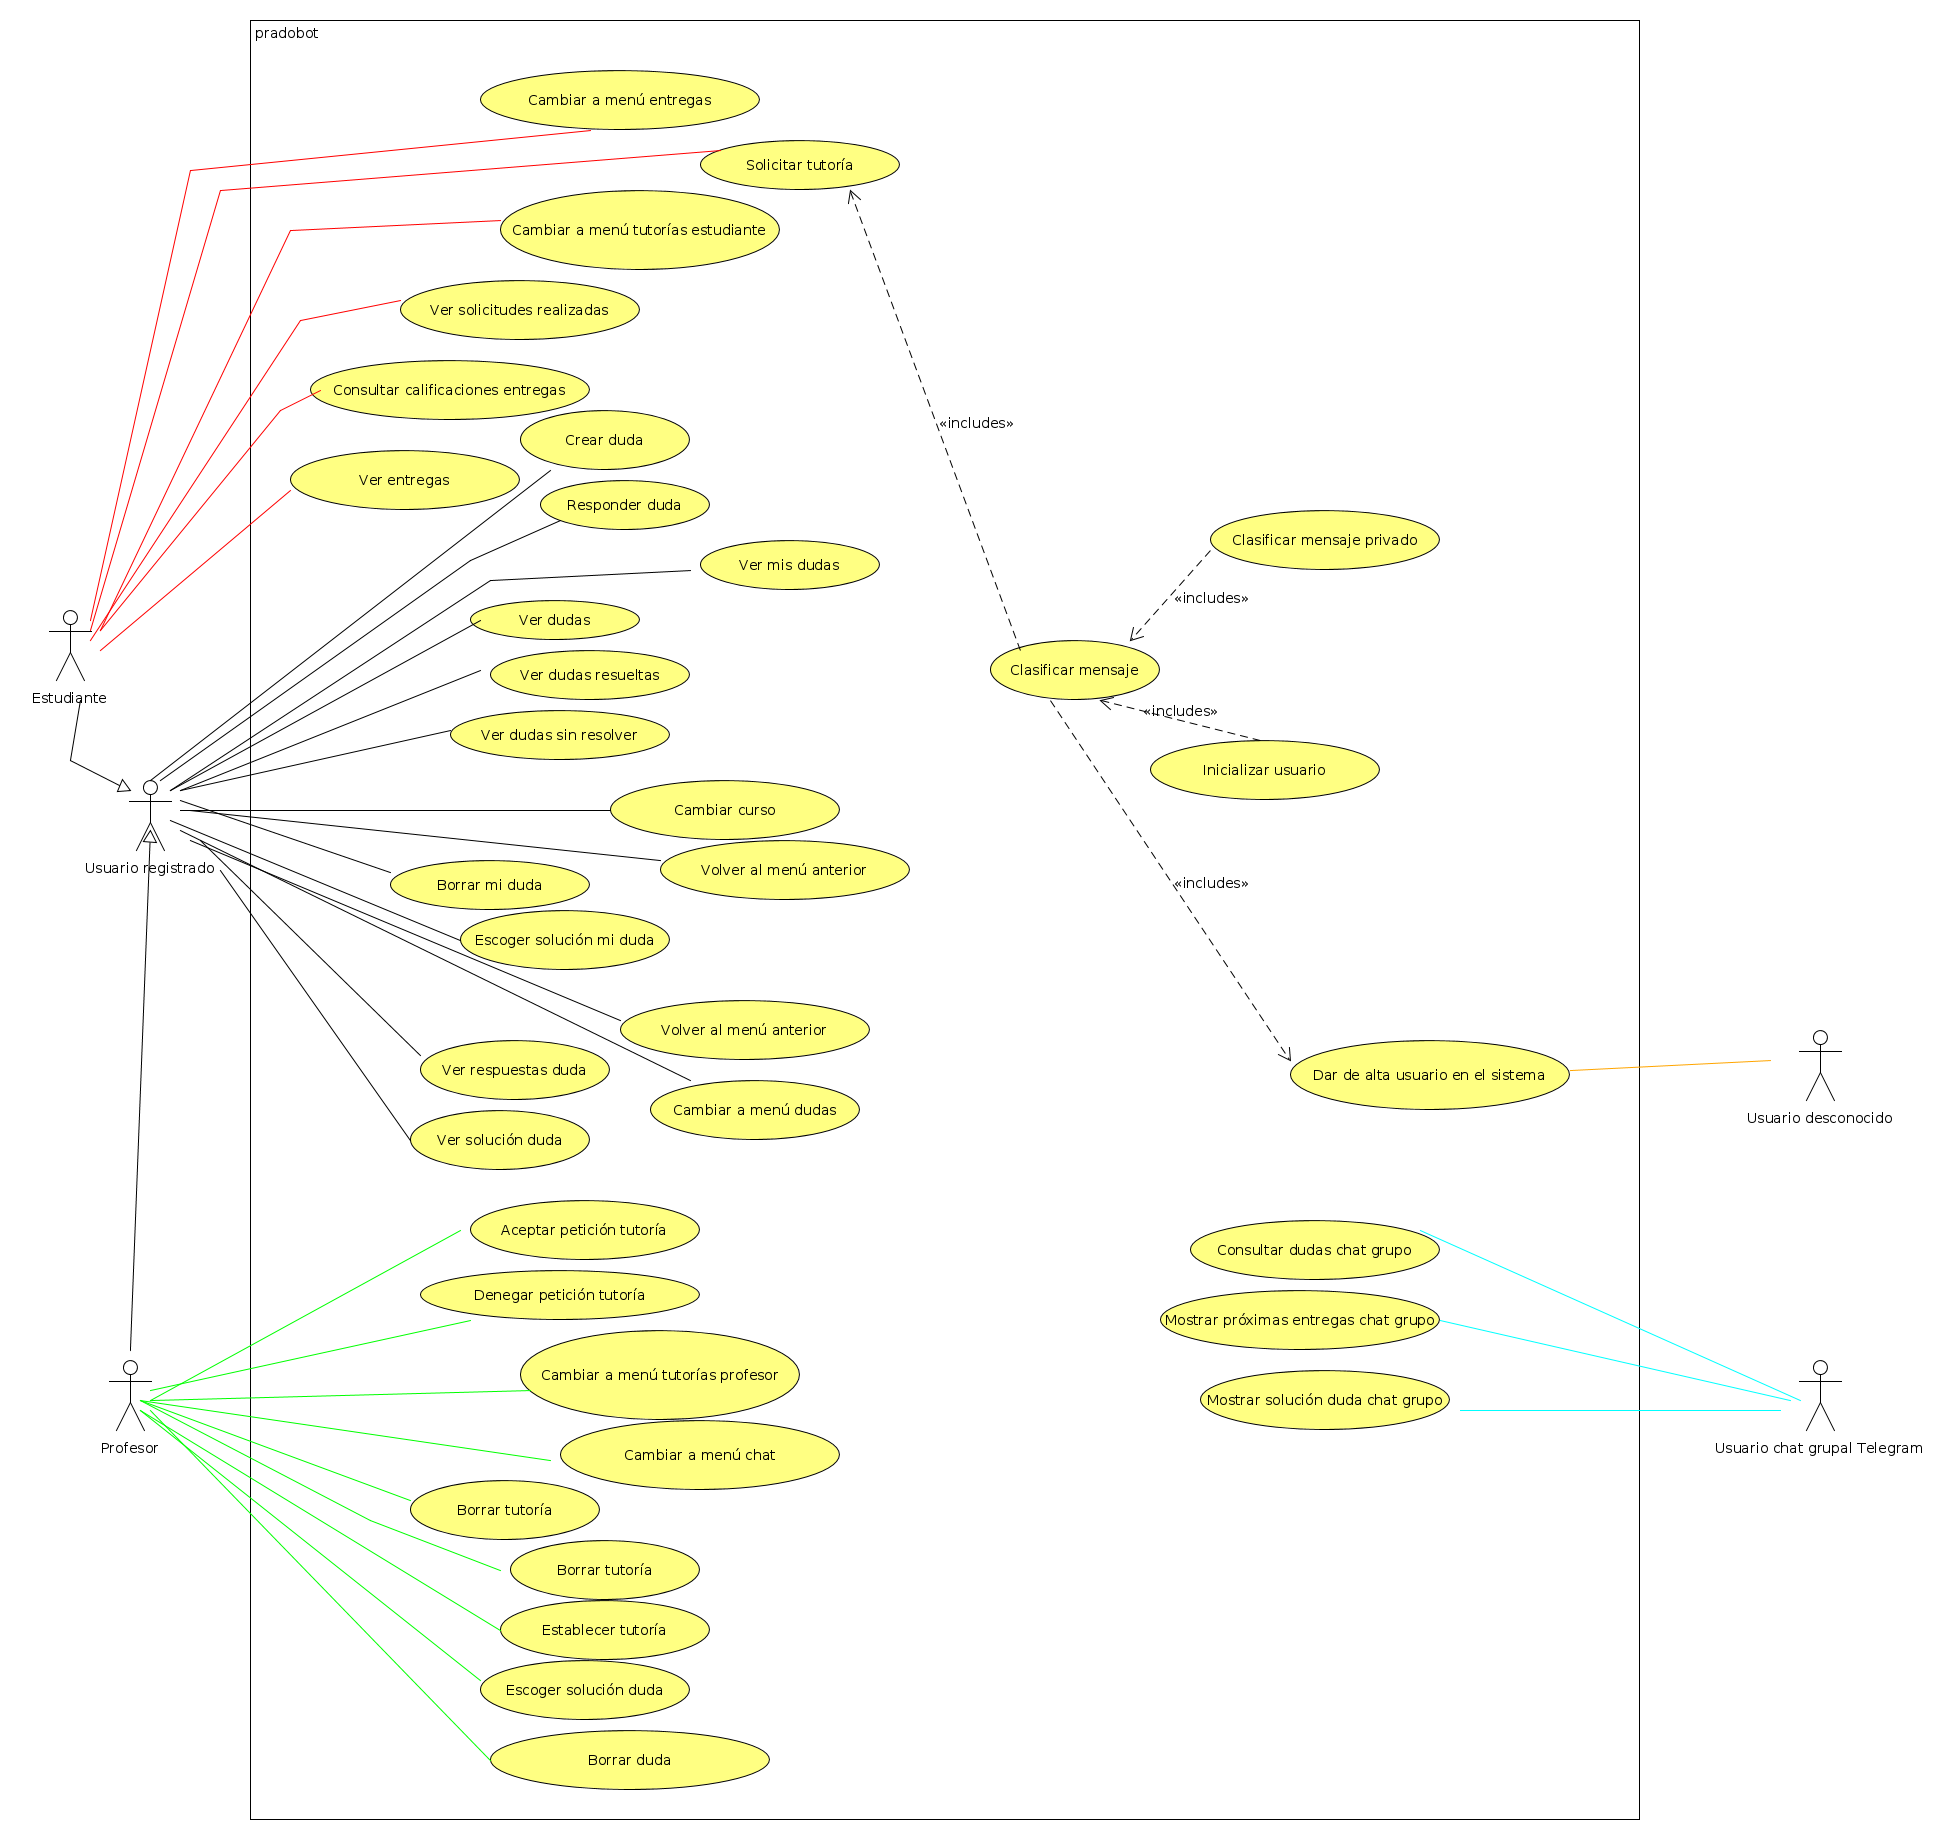
\includegraphics[scale=0.2]{imagenes/diagramas/diagrama_caso_uso.png}  %el parámetro scale permite agrandar o achicar la imagen. En el nombre de archivo puede especificar directorios

\caption{Diagrama de los casos de uso más relevantes del sistema}\label{figura10}
\end{figure}

Podemos observar las funciones comunes que comparten todos los usuarios registrados del sistema, así como las que son especificas de cada rol. Por ejemplo, algo exclusivo del profesor es el establecimiento de las tutorías, mientras que algo único que puede hacer el estudiante es solicitarlas.


\subsection{Descripción casos uso}

He optado por realizar dos tipos de CUs unos más cercanos a los CU Reales, que muestran algunos detalles más cercanos al diseño y otros, bastante más abstractos, cuyo enfoque está en mostrar la interación del usuario con el programa. El objetivo, es que haya equilibrio entre abstracción y las peculiaridades de un programa tipo bot, cuyo funcionamiento depende fuertemente del contexto en el que se recibe un mensaje del usuario.

\begin{table}[H]

\begin{tabular}{|c|m{10cm}|}
\hline\rowcolor{Gray}
{\bf CU-1.1 } & { Clasificar mensaje.}\\
\hline
{\bf Actores } & { Estudiante, Profesor} \\
\hline\rowcolor{Gray}
{\bf Tipo } & { Primario,  Real} \\
\hline
{\bf Referencias }& {CU-1.2 (Clasificar mensaje privado)} \\
\hline\rowcolor{Gray}
{\bf Precondición }& {Bot haya recibido un mensaje} \\
\hline
{\bf Postcondición }& {}\\
\hline\rowcolor{Gray}
{\bf Autor }& { Luis Gil Guijarro}  \\
\hline
{\bf Versión }& { 1.0} \\
\hline\rowcolor{Gray}
{\bf Fecha }& { 10-05-17} \\
\hline
\end{tabular}

\end{table}

\begin{table}[H]

\begin{tabular}{|m{10cm}|}
\hline\rowcolor{Gray}
{\bf Propósito}\\
\hline
{Clasificar un mensaje recibido desde Telegram para determinar si procede de un chat individual o de uno grupal.} \\
\hline

\end{tabular}


\end{table}

\begin{table}[H]

\begin{tabular}{|m{10cm}|}
\hline\rowcolor{Gray}
{\bf Resumen}\\
\hline
{El bot recibe un mensaje y lo clasifica dependiendo de si procede de un chat privado o de uno grupal.} \\
\hline

\end{tabular}



\end{table}

    \begin{table}[!ht]
	\begin{tabular}{|l|l|l|l|}
	  \hline\rowcolor{Gray}
	  \multicolumn{4}{|c|}{{\bf Curso normal}}
	  \\ \hline
	  \multicolumn{2}{|c|}{{\bf Actor}} & \multicolumn{2}{c|}{{\bf Sistema}}
	  \\ \hline

	  &
	  &
	  {\textbf 1} &
	  \begin{tabular}[c]{@{}l@{}}
	    El bot recibe el mensaje.
	  \end{tabular}
	  \\ \hline	  &
	  &
	  {\textbf 2} &
	  \begin{tabular}[c]{@{}l@{}}
	    El bot comprueba si el mensaje procede de un\\ chat grupal o de uno privado.
	  \end{tabular}
	  \\ \hline	  &
	  &
	  {\textbf 3} &
	  \begin{tabular}[c]{@{}l@{}}
	    El bot clasifica el mensaje como privado.
	  \end{tabular}
	  \\ \hline	  &
	  &
	  {\textbf 4} &
	  \begin{tabular}[c]{@{}l@{}}
	    Incluir( CU-1.2, Clasificar mensaje privado)
	  \end{tabular}
	  \\ \hline	  
	\end{tabular}
	\caption{Curso normal de CU-1.1. Clasificar mensaje.}
	\label{table:cn_cu_1.1}
    \end{table}

    \begin{table}[!ht]
	\begin{tabular}{|l|l|l|l|}
	  \hline\rowcolor{Gray}
	  \multicolumn{2}{|c|}{{\bf Cursos alternos}}
	  \\ \hline
	  {\textbf 3a} & 
	  \begin{tabular}[c]{@{}l@{}}
	    El bot clasifica el mensaje como grupal\\ Incluir( CU-1.4, Clasificar mensaje grupal) \\Fin CU.
	  \end{tabular} 
	  
	  
	  \\ \hline
	\end{tabular}
	\caption{Cursos alternos de CU-1.1. Clasificar mensaje.}
	\label{table:ca_cu_1.1}
    \end{table}
    
    
%%%%%%%%%%%%%%%%%%%%%%%%%%%%%%%%%%%%%%%%%%%%%%%%%%%%%%%
    
\begin{table}[!ht]

\begin{tabular}{|c|m{10cm}|}
\hline\rowcolor{Gray}
{\bf CU-1.2 } & { Clasificar mensaje privado}\\
\hline
{\bf Actores } & { Estudiante, Profesor} \\
\hline\rowcolor{Gray}
{\bf Tipo } & { Primario, Real} \\
\hline
{\bf Referencias }& {CU-1.3 (Inicializar usuario)} \\
\hline\rowcolor{Gray}
{\bf Precondición }& {El bot haya recibido un mensaje. El mensaje debe proceder desde un chat privado de Telegram} \\
\hline
{\bf Postcondición }& {}\\
\hline\rowcolor{Gray}
{\bf Autor }& { Luis Gil Guijarro}  \\
\hline
{\bf Versión }& { 1.0} \\
\hline\rowcolor{Gray}
{\bf Fecha }& { 10-05-17} \\
\hline
\end{tabular}

\end{table}

\begin{table}[!ht]

\begin{tabular}{|m{10cm}|}
\hline\rowcolor{Gray}
{\bf Propósito}\\
\hline
{Clasificar un mensaje procedente de un chat privado} \\
\hline

\end{tabular}


\end{table}

\begin{table}[!ht]

\begin{tabular}{|m{10cm}|}
\hline\rowcolor{Gray}
{\bf Resumen}\\
\hline
{El bot recibe un mensaje determinando el tipo de usuario que le manda el mensaje y si es la primera vez que recibe un mensaje de este usuario } \\
\hline

\end{tabular}



\end{table}

    \begin{table}[!ht]
	\begin{tabular}{|l|l|l|l|}
	  \hline\rowcolor{Gray}
	  \multicolumn{4}{|c|}{{\bf Curso normal}}
	  \\ \hline
	  \multicolumn{2}{|c|}{{\bf Actor}} & \multicolumn{2}{c|}{{\bf Sistema}}
	  \\ \hline

	  &
	  &
	  {\textbf 1} &
	  \begin{tabular}[c]{@{}l@{}}
	    Obtiene todos los usuarios\\ que han usuado el\\ bot desde que éste empezó a funcionar
	  \end{tabular}
	  	  \\ \hline

	  &
	  &
	  {\textbf 2} &
	  \begin{tabular}[c]{@{}l@{}}
	    Obtiene al usuario del mensaje.
	  \end{tabular}
	  \\ \hline	  &
	  &
	  {\textbf 3} &
	  \begin{tabular}[c]{@{}l@{}}
	    Comprueba si el usuario que le ha mandado el mensaje\\ está entre ellos.
	  \end{tabular}
	  \\ \hline	  &
	  &
	  {\textbf 4} &
	  \begin{tabular}[c]{@{}l@{}}
	    Comprueba si ha acabo de procesarse el último\\ mensaje que envió el usuario.
	  \end{tabular}
	  \\ \hline	  &
	  &
	  {\textbf 5} &
	  \begin{tabular}[c]{@{}l@{}}
	    Obtiene el menú devuelto por el último menú\\ utilizado por el usuario.
	  \end{tabular}
	  \\ \hline	  &
	  &
	  {\textbf 6} &
	  \begin{tabular}[c]{@{}l@{}}
	    Pasa el nuevo mensaje del usuario al\\ menú devuelto.
	  \end{tabular}
	  \\ \hline
	\end{tabular}
	\caption{Curso normal de CU-1.2. Clasificar mensaje privado.}
	\label{table:cn_cu_1.2}
    \end{table}

    \begin{table}[!ht]
	\begin{tabular}{|l|l|l|l|}
	  \hline\rowcolor{Gray}
	  \multicolumn{2}{|c|}{{\bf Cursos alternos}}
	  \\ \hline
	  {\textbf 3a} & 
	  \begin{tabular}[c]{@{}l@{}}
	    	    El usuario no le ha mandado un \\mensaje al bot desde que éste  \\ empezó a funcionar\\. Incluir (CU-1.3, inicializar usuario)
 . Fin CU.
	  \end{tabular} 
	  \\ \hline
	  {\textbf 4a} & 
	  \begin{tabular}[c]{@{}l@{}}
	    La acción que ejecutó el usuario\\ en su último mensaje no se \\ ha acabado de ejecutar\\. Bot le pide que espere . Fin CU.
	  \end{tabular} 
	  \\ \hline
	\end{tabular}
	\caption{Cursos alternos de CU-1.2. Clasificar mensaje privado.}
	\label{table:ca_cu_1.2}
    \end{table}
    


%%%%%%%%%%%%%%%%%%%%%



\begin{table}[!ht]

\begin{tabular}{|c|m{10cm}|}
\hline\rowcolor{Gray}
{\bf CU-1.3 } & {Inicializar usuario}\\
\hline
{\bf Actores } & { Estudiante, Profesor} \\
\hline\rowcolor{Gray}
{\bf Tipo } & { Primario, Real} \\
\hline
{\bf Referencias }& {} \\
\hline\rowcolor{Gray}
{\bf Precondición }& {El usuario que le manda el mensaje al bot no le haya mandado un mensaje anteriormente desde que éste empezó a ejecutarse} \\
\hline
{\bf Postcondición }& {El usuario será añadido a la lista de usuarios que están utilizando el bot}\\
\hline\rowcolor{Gray}
{\bf Autor }& { Luis Gil Guijarro}  \\
\hline
{\bf Versión }& { 1.0} \\
\hline\rowcolor{Gray}
{\bf Fecha }& { 10-05-17} \\
\hline
\end{tabular}

\end{table}

\begin{table}[!ht]

\begin{tabular}{|m{10cm}|}
\hline\rowcolor{Gray}
{\bf Propósito}\\
\hline
{Asignarle un menú de inicio al usuario que le ha mandado el mensaje} \\
\hline

\end{tabular}


\end{table}

\begin{table}[!ht]

\begin{tabular}{|m{10cm}|}
\hline\rowcolor{Gray}
{\bf Resumen}\\
\hline
{El bot determina si el usuario está registrado en el sistema y le asigna un menú de inicio. } \\
\hline

\end{tabular}



\end{table}

    \begin{table}[!ht]
	\begin{tabular}{|l|l|l|l|}
	  \hline\rowcolor{Gray}
	  \multicolumn{4}{|c|}{{\bf Curso normal}}
	  \\ \hline
	  \multicolumn{2}{|c|}{{\bf Actor}} & \multicolumn{2}{c|}{{\bf Sistema}}
	  \\ \hline

	  &
	  &
	  {\textbf 1} &
	  \begin{tabular}[c]{@{}l@{}}
	    Bot comprueba si el usuario está registrado\\ en el sistema.
	  \end{tabular}
	  \\ \hline	  &
	  &
	  {\textbf 2} &
	  \begin{tabular}[c]{@{}l@{}}
	    El bot obtiene una lista de cursos en los que\\ se encuentra matriculado el usuario.
	  \end{tabular}
	  \\ \hline	  &
	  &
	  {\textbf 3} &
	  \begin{tabular}[c]{@{}l@{}}
	    El bot asigna como curso activo del usuario\\ al primer curso de la lista.
	  \end{tabular}
	  \\ \hline	  &
	  &
	  {\textbf 4} &
	  \begin{tabular}[c]{@{}l@{}}
	    El bot obtiene el menú inicial del profesor.
	  \end{tabular}
	  \\ \hline	  &
	  &
	  {\textbf 5} &
	  \begin{tabular}[c]{@{}l@{}}
	    El bot le muestra al usuario el menú\\ principal del profesor.
	  \end{tabular}
	  \\ \hline

	\end{tabular}
	\caption{Curso normal de CU-1.3. Inicializar usuario.}
	\label{table:cn_cu_1.3}
    \end{table}

    \begin{table}[!ht]
	\begin{tabular}{|l|l|l|l|}
	  \hline\rowcolor{Gray}
	  \multicolumn{2}{|c|}{{\bf Cursos alternos}}
	  \\ \hline
	  {\textbf 2a} & 
	  \begin{tabular}[c]{@{}l@{}}
	    El usuario no está registrado en el sistema. Obtiene\\ el menú encargado de iniciar usuarios desconocidos.\\ Muestra este menú al usuario. Fin CU.
	  \end{tabular} 
	  
	  
	  \\ \hline
	  	  {\textbf 4a} & 
	  \begin{tabular}[c]{@{}l@{}}
	    El usuario es un estudiante. Obtiene el menú inicial\\ del estudiante y se lo muestra. Fin CU.
	  \end{tabular} 
	  
	  
	  \\ \hline
	\end{tabular}
	\caption{Cursos alternos de CU-1.3. Inicializar usuario.}
	\label{table:ca_cu_1.3}
    \end{table}
    


%%%%%%%%%%%%%%%%%%%%%%%%%%%%%%%%%%%%%%%%%%%




\begin{table}[!ht]

\begin{tabular}{|c|m{10cm}|}
\hline\rowcolor{Gray}
{\bf CU-1.4 } & { Cambiar curso.}\\
\hline
{\bf Actores } & { Usuario Registrado} \\
\hline\rowcolor{Gray}
{\bf Tipo } & { Primario, Real} \\
\hline
{\bf Referencias }& {CU-1.1 (Clasificar mensaje)} \\
\hline\rowcolor{Gray}
{\bf Precondición }& {} \\
\hline
{\bf Postcondición }& {El usuario habrá cambiado el curso sobre el que actúan los mensajes que le envíe al bot.}\\
\hline\rowcolor{Gray}
{\bf Autor }& { Luis Gil Guijarro}  \\
\hline
{\bf Versión }& { 1.0} \\
\hline\rowcolor{Gray}
{\bf Fecha }& { 10-05-17} \\
\hline
\end{tabular}

\end{table}

\begin{table}[!ht]

\begin{tabular}{|m{10cm}|}
\hline\rowcolor{Gray}
{\bf Propósito}\\
\hline
{Que un usuario que utilize el bot pueda variar el curso sobre el cual actúan sus mensajes} \\
\hline

\end{tabular}


\end{table}

\begin{table}[!ht]

\begin{tabular}{|m{10cm}|}
\hline\rowcolor{Gray}
{\bf Resumen}\\
\hline
{El usuario selecciona en el menú que le esté mostrando el bot, que desea cambiar de curso. El bot le muestra los cursos accesibles para el usuario, el usuario escoge uno y el bot cambia el curso del usuario.} \\
\hline

\end{tabular}



\end{table}


    \begin{table}[!ht]
	\begin{tabular}{|l|l|l|l|}
	  \hline\rowcolor{Gray}
	  \multicolumn{4}{|c|}{{\bf Curso normal}}
	  \\ \hline
	  \multicolumn{2}{|c|}{{\bf Actor}} & \multicolumn{2}{c|}{{\bf Sistema}}
	  \\ \hline
	  {\textbf 1} & 
	  \begin{tabular}[c]{@{}l@{}}
	    El usuario selecciona en el\\ menú que tenga activo\\ que desea cambiar de curso.
	  \end{tabular} 
	  &
	  &
	  \\ \hline
	  &
	  &
	  {\textbf 2} &
	  \begin{tabular}[c]{@{}l@{}}
	    Incluir(CU-1.1, Clasificar mensaje)
	  \end{tabular}
	  \\ \hline
	  	  &
	  &
	  {\textbf 3} &
	  \begin{tabular}[c]{@{}l@{}}
	    El bot detecta que el usuario\\ ha pulsado cambiar de curso.
	  \end{tabular}
	  \\ \hline
	  	  	  &
	  &
	  {\textbf 4} &
	  \begin{tabular}[c]{@{}l@{}}
	    El bot obtiene todos los cursos\\ para los cuales está dado de\\ alta el usuario.
	  \end{tabular}
	  \\ \hline
	  &
	  &
	  {\textbf 5} &
	  \begin{tabular}[c]{@{}l@{}}
	    El bot muestra todos los cursos al usuario.
	  \end{tabular}
	  \\ \hline	  
	  {\textbf 6} & 
	  \begin{tabular}[c]{@{}l@{}}
	    El usuario elige\\ un curso\\.
	  \end{tabular} 
	  &
	  &
	  \\ \hline
	  &
	  &
	  {\textbf 7} &
	  \begin{tabular}[c]{@{}l@{}}
	    Incluir(CU-1.1, Clasificar mensaje)
	  \end{tabular}
	  \\ \hline	  
	  
	  	  &
	  &
	  {\textbf 8} &
	  \begin{tabular}[c]{@{}l@{}}
	    El bot identifica al curso \\seleccionado por el usuario.
	  \end{tabular}
	  \\ \hline
	  	  	  &
	  &
	  {\textbf 9} &
	  \begin{tabular}[c]{@{}l@{}}
	    El bot cambia el curso para el usuario.
	  \end{tabular}
	  \\ \hline
	  	  	  &
	  &
	  {\textbf 10} &
	  \begin{tabular}[c]{@{}l@{}}
	    El bot informa al usurio del cambio de curso.\\
	  \end{tabular}
	  \\ \hline
	\end{tabular}
	\caption{Curso normal de CU-1.4. Cambiar de curso.}
	\label{table:cn_cu_1.4}
    \end{table}



%%%%%%%%%%%%%%%%%%%%%%%%%%%%%%%%%%%%%%%%%%%%
\clearpage
\begin{table}[!ht]

\begin{tabular}{|c|m{10cm}|}
\hline\rowcolor{Gray}
{\bf CU-2 } & { Dar de alta usuario en el sistema.}\\
\hline
{\bf Actores } & { Usuario sin identificar} \\
\hline\rowcolor{Gray}
{\bf Tipo } & { Primario,  Real} \\
\hline
{\bf Referencias }& {CU-1.1 (Clasificar mensaje)} \\
\hline\rowcolor{Gray}
{\bf Precondición }& {El usuario no este registrado en el sistema.} \\
\hline
{\bf Postcondición }& {Se habrá registrado un nuevo usuario en el sistema.}\\
\hline\rowcolor{Gray}
{\bf Autor }& { Luis Gil Guijarro}  \\
\hline
{\bf Versión }& { 1.0} \\
\hline\rowcolor{Gray}
{\bf Fecha }& { 10-05-17} \\
\hline
\end{tabular}

\end{table}

\begin{table}[!ht]

\begin{tabular}{|m{10cm}|}
\hline\rowcolor{Gray}
{\bf Propósito}\\
\hline
{Para utilizar el bot es necesario que el usuario se indentifique como usuario autorizado, para lo cual es necesario que pruebe que tiene acceso a los recursos de la instancia de Moodle.} \\
\hline

\end{tabular}


\end{table}

\begin{table}[!ht]

\begin{tabular}{|m{10cm}|}
\hline\rowcolor{Gray}
{\bf Resumen}\\
\hline
{El usuario manda un mensaje al bot y éste le pide que se identifique introduciendo el email y contraseña que utiliza en Moodle, el usuario los introduce y el bot registra al usuario} \\
\hline

\end{tabular}



\end{table}


    \begin{table}[!ht]
	\begin{tabular}{|l|l|l|l|}
	  \hline\rowcolor{Gray}
	  \multicolumn{4}{|c|}{{\bf Curso normal}}
	  \\ \hline
	  \multicolumn{2}{|c|}{{\bf Actor}} & \multicolumn{2}{c|}{{\bf Sistema}}
	  \\ \hline
	  {\textbf 1} & 
	  \begin{tabular}[c]{@{}l@{}}
	    El usuario manda un mensaje al bot.
	  \end{tabular} 
	  &
	  &
	  \\ \hline
	  &
	  &
	  {\textbf 2} &
	  \begin{tabular}[c]{@{}l@{}}
	    Incluir(CU-1.1, Clasificar mensaje)
	  \end{tabular}
	  \\ \hline
	  	  &
	  &
	  {\textbf 3} &
	  \begin{tabular}[c]{@{}l@{}}
	    El bot le solicita que introduzca el\\ email que utiliza en Moodle.
	  \end{tabular}
	  \\ \hline
	  	  {\textbf 4} & 
	  \begin{tabular}[c]{@{}l@{}}
	   El usuario manda un mensaje al bot\\ indicando su email.
	  \end{tabular} 
	  &
	  &
	  
	  \\ \hline
	  &
	  &
	  {\textbf 5} &
	  \begin{tabular}[c]{@{}l@{}}
	    Incluir(CU-1.1, Clasificar mensaje)
	  \end{tabular}
	  \\ \hline	  
	  &
	  &
	  {\textbf 6} &
	  \begin{tabular}[c]{@{}l@{}}
	    El bot le solicita que introduzca la\\ contraseña que utiliza para Moodle.
	  \end{tabular}
	  \\ \hline
	  	  	  {\textbf 7} & 
	  \begin{tabular}[c]{@{}l@{}}
	   El usuario introduce la contraseña.
	  \end{tabular} 
	  &
	  &	  
	  \\ \hline
	  &
	  &
	  {\textbf 8} &
	  \begin{tabular}[c]{@{}l@{}}
	    Incluir(CU-1.1, Clasificar mensaje privado)
	  \end{tabular}
	  \\ \hline	  
	  
	  	  &
	  &
	  {\textbf 9} &
	  \begin{tabular}[c]{@{}l@{}}
	    El bot solicita la token de usuario\\ a la instancia de Moodle\\.
	  \end{tabular}
	  \\ \hline
	  	  	  &
	  &
	  {\textbf 10} &
	  \begin{tabular}[c]{@{}l@{}}
	    El bot solicita los cursos accesibles\\ para el usuario a la instancia\\ de Moodle.
	  \end{tabular}
	  \\ \hline
	  	  	  &
	  &
	  {\textbf 11} &
	  \begin{tabular}[c]{@{}l@{}}
	    El bot registra al usuario en el sistema.\\
	  \end{tabular}
	  \\ \hline
	  
	  	  
	  	  &
	  &
	  {\textbf 12} &
	  \begin{tabular}[c]{@{}l@{}}
	    El bot establece como curso activo\\ al primero de los obtenidos.
	  \end{tabular}
	  \\ \hline
	  	  	  &
	  &
	  {\textbf 13} &
	  \begin{tabular}[c]{@{}l@{}}
	    El bot obtiene el menú principal del profesor\\.
	  \end{tabular}
	  \\ \hline
	  	  	  &
	  &
	  {\textbf 14} &
	  \begin{tabular}[c]{@{}l@{}}
	    El bot establece el menú principal del profesor\\ como menú a mostrar al \\usuario.
	  \end{tabular}
	  \\ \hline	  
	  	  	  &
	  &
	  {\textbf 15} &
	  \begin{tabular}[c]{@{}l@{}}
	    El bot le muestra el menú principal al usuario.
	  \end{tabular}
	  \\ \hline		  
	  
	  	  
	  &
	  &
	  {\textbf 16} &
	  \begin{tabular}[c]{@{}l@{}}
	    El bot le indica que que puede\\ empezar a usarlo.
	  \end{tabular}
	  \\ \hline
	\end{tabular}
	\caption{Curso normal de CU-2. Dar de alta usuario en el sistema.}
	\label{table:cn_cu_2}
    \end{table}

    \begin{table}[!ht]
	\begin{tabular}{|l|l|l|l|}
	  \hline\rowcolor{Gray}
	  \multicolumn{2}{|c|}{{\bf Cursos alternos}}
	  \\ \hline
	  {\textbf 10a} & 
	  \begin{tabular}[c]{@{}l@{}}
	    Moodle le dice que los datos introducidos\\ son erroneos\\. Bot manda mensaje de error al\\ usuario. Fin CU.
	  \end{tabular} 
	  \\ \hline
	  {\textbf 11a} & 
	  \begin{tabular}[c]{@{}l@{}}
	    El usuario no puede acceder a ningún\\ curso a través de la API\\ de Moodle, bot manda mensaje de error\\.  Fin CU.
	  \end{tabular}	  
	  
	  \\ \hline
	  	  {\textbf 13a} & 
	  \begin{tabular}[c]{@{}l@{}}
	    El usuario es un estudiante\\ el bot obtiene el menú principal  \\ para los estudiantes. \\Se lo muestra al estudiante. \\Indica que puede empezar a utilizar\\ el bot. Fin CU.
	  \end{tabular}	  
	  
	  \\ \hline
	\end{tabular}
	\caption{Cursos alternos de CU-2. Dar de alta usuario en el sistema.}
	\label{table:ca_cu_2}
    \end{table}
    

%%%%%%%%%%%%%%%%%%%%%%%%%%%%%%%%%%%%%%%%%%%%






%%%%%%%%%%%%%%%%%%%%%%%%%%%%%%%%%%%%%%%%%%%%






    \begin{table}[!ht]


    
\begin{tabular}{|c|m{10cm}|}
\hline\rowcolor{Gray}
{\bf CU-3.1 } & {Cambiar a menú entregas}\\
\hline
{\bf Actores } & {  Estudiante } \\
\hline\rowcolor{Gray}
{\bf Tipo } & { Primario, Esencial} \\
\hline
{\bf Referencias }& {} \\
\hline\rowcolor{Gray}
{\bf Precondición }& 

	  \begin{tabular}[c]{@{}l@{}}
	    Estudiante se encuentre en el menú principal\\ del estudiante.
	  \end{tabular}  
 \\
\hline
{\bf Postcondición }& {}\\
\hline\rowcolor{Gray}
{\bf Autor }& { Luis Gil Guijarro}  \\
\hline
{\bf Versión }& { 1.0} \\
\hline\rowcolor{Gray}
{\bf Fecha }& { 10-05-17} \\
\hline
\end{tabular}

\end{table}

\begin{table}[!ht]

\begin{tabular}{|m{10cm}|}
\hline\rowcolor{Gray}
{\bf Propósito}\\
\hline
{Que el estudiante pueda cambiar desde el menú principal del estudiante al de entregas.} \\
\hline

\end{tabular}


\end{table}

\begin{table}[!ht]

\begin{tabular}{|m{10cm}|}
\hline\rowcolor{Gray}
{\bf Resumen}\\
\hline
{El estudiante le indica al bot que desea cambiar al menú de entregas y el bot lo cambia} \\
\hline

\end{tabular}



\end{table}

    \begin{table}[!ht]
	\begin{tabular}{|l|l|l|l|}
	  \hline\rowcolor{Gray}
	  \multicolumn{4}{|c|}{{\bf Curso normal}}
	  \\ \hline
	  \multicolumn{2}{|c|}{{\bf Actor}} & \multicolumn{2}{c|}{{\bf Sistema}}
	  \\ \hline
	  	  {\textbf 1} & 
	  \begin{tabular}[c]{@{}l@{}}
	   El estudiante selecciona al menú\\ de entregas.
	  \end{tabular} 
	  &
	  &
	  \\ \hline
	   & 
	   &
	  	  {\textbf 2} &
	  \begin{tabular}[c]{@{}l@{}}
	    El bot muestra al estudiante el\\ menú de entregas. 
	  \end{tabular}
 \\ \hline  

	\end{tabular}
	\caption{Curso normal de CU-3.1. Cambiar a menú entregas.}
	\label{table:cn_cu_3.1}
    \end{table}






%%%%%%%%%%%%%%%%%%%%%%%%%%%%%%%%%%%%%%%%%%%


    \begin{table}[!ht]


    
\begin{tabular}{|c|m{10cm}|}
\hline\rowcolor{Gray}
{\bf CU-3.2 } & {Cambiar a menú tutorías}\\
\hline
{\bf Actores } & {  Estudiante } \\
\hline\rowcolor{Gray}
{\bf Tipo } & { Primario, Esencial} \\
\hline
{\bf Referencias }& {} \\
\hline\rowcolor{Gray}
{\bf Precondición }& 

	  \begin{tabular}[c]{@{}l@{}}
	    Estudiante se encuentre en el menú principal\\ del estudiante.
	  \end{tabular}  
 \\
\hline
{\bf Postcondición }& {El estudiante ahora se encontrará en el menú de tutorías}\\
\hline\rowcolor{Gray}
{\bf Autor }& { Luis Gil Guijarro}  \\
\hline
{\bf Versión }& { 1.0} \\
\hline\rowcolor{Gray}
{\bf Fecha }& { 10-05-17} \\
\hline
\end{tabular}

\end{table}

\begin{table}[!ht]

\begin{tabular}{|m{10cm}|}
\hline\rowcolor{Gray}
{\bf Propósito}\\
\hline
{Que el estudiante pueda cambiar desde el menú principal del estudiante al menú de tutorías de estudiantes.} \\
\hline

\end{tabular}


\end{table}

\begin{table}[!ht]

\begin{tabular}{|m{10cm}|}
\hline\rowcolor{Gray}
{\bf Resumen}\\
\hline
{El estudiante le indica al bot que desea cambiar al menú de tutorías y el bot lo cambia} \\
\hline

\end{tabular}



\end{table}

    \begin{table}[!ht]
	\begin{tabular}{|l|l|l|l|}
	  \hline\rowcolor{Gray}
	  \multicolumn{4}{|c|}{{\bf Curso normal}}
	  \\ \hline
	  \multicolumn{2}{|c|}{{\bf Actor}} & \multicolumn{2}{c|}{{\bf Sistema}}
	  \\ \hline
	  	  {\textbf 1} & 
	  \begin{tabular}[c]{@{}l@{}}
	   El estudiante selecciona al\\ menú de tutorías.
	  \end{tabular} 
	  &
	  &
	  \\ \hline
	  	   & 
	   &
	  	  {\textbf 2} &
	  \begin{tabular}[c]{@{}l@{}}
	    El bot cambia al estudiante el\\ menú de tutorías. 
	  \end{tabular}
	  	  	  \\ \hline

	   & 
	   &
	  	  {\textbf 3} &
	  \begin{tabular}[c]{@{}l@{}}
	    El bot muestra al estudiante el\\ menú de tutorías. 
	  \end{tabular}
 \\ \hline  

	\end{tabular}
	\caption{Curso normal de CU-3.2. Cambiar a menú tutorías.}
	\label{table:cn_cu_3.2}
    \end{table}



%%%%%%%%%%%%%%%%%%%%%%%%%%%%%%%%%%%%%%%%%%%%
\clearpage

\begin{table}[!ht]
\begin{tabular}{|c|m{10cm}|}
\hline\rowcolor{Gray}
{\bf CU-3.3 } & {Cambiar a menú tutorías}\\
\hline
{\bf Actores } & {  Profesor } \\
\hline\rowcolor{Gray}
{\bf Tipo } & { Primario, Esencial} \\
\hline
{\bf Referencias }& {} \\
\hline\rowcolor{Gray}
{\bf Precondición }& 

	  \begin{tabular}[c]{@{}l@{}}
	    Profesor esté en el menú principal\\ de profesores.
	  \end{tabular}  
 \\
\hline
{\bf Postcondición }& {El profesor estará  en el menú de tutorías para profesores}\\
\hline\rowcolor{Gray}
{\bf Autor }& { Luis Gil Guijarro}  \\
\hline
{\bf Versión }& { 1.0} \\
\hline\rowcolor{Gray}
{\bf Fecha }& { 10-05-17} \\
\hline
\end{tabular}

\end{table}

\begin{table}[!ht]

\begin{tabular}{|m{10cm}|}
\hline\rowcolor{Gray}
{\bf Propósito}\\
\hline
{Que el profesor pueda cambiar desde el menú principal de los profesores al menú de tutorías para los profesores} \\
\hline

\end{tabular}


\end{table}

\begin{table}[!ht]

\begin{tabular}{|m{10cm}|}
\hline\rowcolor{Gray}
{\bf Resumen}\\
\hline
{El profesor le indica al bot que lo cambie al menú de tutorías y el bot lo cambia} \\
\hline

\end{tabular}



\end{table}

    \begin{table}[!ht]
	\begin{tabular}{|l|l|l|l|}
	  \hline\rowcolor{Gray}
	  \multicolumn{4}{|c|}{{\bf Curso normal}}
	  \\ \hline
	  \multicolumn{2}{|c|}{{\bf Actor}} & \multicolumn{2}{c|}{{\bf Sistema}}
	  \\ \hline
	  	  {\textbf 1} & 
	  \begin{tabular}[c]{@{}l@{}}
	   El profesor selecciona el \\menú de tutorías.
	  \end{tabular} 
	  &
	  &
	  \\ \hline
	  	   & 
	   &
	  	  {\textbf 2} &
	  \begin{tabular}[c]{@{}l@{}}
	    El bot cambia al profesor al \\menú de tutorías. 
	  \end{tabular}
	  	  	  \\ \hline

	   & 
	   &
	  	  {\textbf 3} &
	  \begin{tabular}[c]{@{}l@{}}
	    El bot muestra al profesor el \\menú de tutorías. 
	  \end{tabular}
 \\ \hline  

	\end{tabular}
	\caption{Curso normal de CU-3.3. Cambiar a menú tutorías.}
	\label{table:cn_cu_3.3}
    \end{table}




\clearpage

%%%%%%%%%%%%%%%%%%%%%%%%%%%%%%%%%%%%%%%%%%%%

\begin{table}[!ht]
\begin{tabular}{|c|m{10cm}|}
\hline\rowcolor{Gray}
{\bf CU-3.4 } & {Cambiar a menú chat}\\
\hline
{\bf Actores } & {  Profesor } \\
\hline\rowcolor{Gray}
{\bf Tipo } & { Primario, Esencial} \\
\hline
{\bf Referencias }& {} \\
\hline\rowcolor{Gray}
{\bf Precondición }& 

	  \begin{tabular}[c]{@{}l@{}}
	    Profesor esté en el menú principal\\ de profesores.
	  \end{tabular}  
 \\
\hline
{\bf Postcondición }& {El profesor estará  en el menú de chat}\\
\hline\rowcolor{Gray}
{\bf Autor }& { Luis Gil Guijarro}  \\
\hline
{\bf Versión }& { 1.0} \\
\hline\rowcolor{Gray}
{\bf Fecha }& { 10-05-17} \\
\hline
\end{tabular}

\end{table}

\begin{table}[!ht]

\begin{tabular}{|m{10cm}|}
\hline\rowcolor{Gray}
{\bf Propósito}\\
\hline
{Que el profesor pueda cambiar desde el menú principal de los profesores al menú de chat de Telegram} \\
\hline

\end{tabular}


\end{table}

\begin{table}[!ht]

\begin{tabular}{|m{10cm}|}
\hline\rowcolor{Gray}
{\bf Resumen}\\
\hline
{El profesor le indica al bot que desea ir al menú de chat y el bot lo cambia} \\
\hline

\end{tabular}



\end{table}

    \begin{table}[!ht]
	\begin{tabular}{|l|l|l|l|}
	  \hline\rowcolor{Gray}
	  \multicolumn{4}{|c|}{{\bf Curso normal}}
	  \\ \hline
	  \multicolumn{2}{|c|}{{\bf Actor}} & \multicolumn{2}{c|}{{\bf Sistema}}
	  \\ \hline
	  	  {\textbf 1} & 
	  \begin{tabular}[c]{@{}l@{}}
	   El profesor selecciona el\\ menú de chat.
	  \end{tabular} 
	  &
	  &
	  \\ \hline
	  	   & 
	   &
	  	  {\textbf 2} &
	  \begin{tabular}[c]{@{}l@{}}
	    El bot cambia al profesor\\ al menú de chat. 
	  \end{tabular}
	  	  	  \\ \hline

	   & 
	   &
	  	  {\textbf 3} &
	  \begin{tabular}[c]{@{}l@{}}
	    El bot muestra al profesor el menú de chat al profesor.. 
	  \end{tabular}
 \\ \hline  

	\end{tabular}
	\caption{Curso normal de CU-3.4. Cambiar a menú chat.}
	\label{table:cn_cu_3.4}
    \end{table}


%%%%%%%%%%%%%%%%%%%%%%%%%%%%%%%%%%%%%%%%%%%%


%%%%%%%%%%%%%%%%%%%%%%%%%%%%%%%%%%%%%%%%%%%%
\clearpage
\begin{table}[!ht]

\begin{tabular}{|c|m{10cm}|}
\hline\rowcolor{Gray}
{\bf CU-3.5 } & {Cambiar a menú dudas}\\
\hline
{\bf Actores } & {  Usuario registrado } \\
\hline\rowcolor{Gray}
{\bf Tipo } & { Primario, Esencial} \\
\hline
{\bf Referencias }& {} \\
\hline\rowcolor{Gray}
{\bf Precondición }& 

	  \begin{tabular}[c]{@{}l@{}}
	    Profesor esté en el menú principal\\ de profesores.
	  \end{tabular}  
 \\
\hline
{\bf Postcondición }& {El usuario se encontrará en el menú de dudas}\\
\hline\rowcolor{Gray}
{\bf Autor }& { Luis Gil Guijarro}  \\
\hline
{\bf Versión }& { 1.0} \\
\hline\rowcolor{Gray}
{\bf Fecha }& { 10-05-17} \\
\hline
\end{tabular}

\end{table}

\begin{table}[!ht]

\begin{tabular}{|m{10cm}|}
\hline\rowcolor{Gray}
{\bf Propósito}\\
\hline
{Que un usuario pueda acceder al menú de dudas.} \\
\hline

\end{tabular}


\end{table}

\begin{table}[!ht]

\begin{tabular}{|m{10cm}|}
\hline\rowcolor{Gray}
{\bf Resumen}\\
\hline
{El usuario indica al bot que desea acceder al menú de dudas, el bot lo cambia y se lo muestra} \\
\hline

\end{tabular}



\end{table}

    \begin{table}[!ht]
	\begin{tabular}{|l|l|l|l|}
	  \hline\rowcolor{Gray}
	  \multicolumn{4}{|c|}{{\bf Curso normal}}
	  \\ \hline
	  \multicolumn{2}{|c|}{{\bf Actor}} & \multicolumn{2}{c|}{{\bf Sistema}}
	  \\ \hline
	  	  {\textbf 1} & 
	  \begin{tabular}[c]{@{}l@{}}
	   El usuario selecciona el\\ menú de dudas.
	  \end{tabular} 
	  &
	  &
	  \\ \hline
	  	   & 
	   &
	  	  {\textbf 2} &
	  \begin{tabular}[c]{@{}l@{}}
	    El bot cambia al usuario\\ al menú de dudas. 
	  \end{tabular}
	  	  	  \\ \hline

	   & 
	   &
	  	  {\textbf 3} &
	  \begin{tabular}[c]{@{}l@{}}
	    El bot muestra al usuario\\ el menú de dudas. 
	  \end{tabular}
 \\ \hline  

	\end{tabular}
	\caption{Curso normal de CU-3.5. Cambiar a menú dudas.}
	\label{table:cn_cu_3.5}
    \end{table}


%%%%%%%%%%%%%%%%%%%%%%%%%%%%%%%%%%%%%%%%%%%%

\clearpage


\begin{table}[!ht]

\begin{tabular}{|c|m{10cm}|}
\hline\rowcolor{Gray}
{\bf CU-3.6 } & {Volver al menú anterior}\\
\hline
{\bf Actores } & {  Usuario registrado } \\
\hline\rowcolor{Gray}
{\bf Tipo } & { Primario, Esencial} \\
\hline
{\bf Referencias }& {} \\
\hline\rowcolor{Gray}
{\bf Precondición }& 

	  \begin{tabular}[c]{@{}l@{}}
	    El usuario no se encuentre en su menú principal
	  \end{tabular}  
 \\
\hline
{\bf Postcondición }& {El usuario se encontrará en el menú inmediatamente anterior que haya visitado}\\
\hline\rowcolor{Gray}
{\bf Autor }& { Luis Gil Guijarro}  \\
\hline
{\bf Versión }& { 1.0} \\
\hline\rowcolor{Gray}
{\bf Fecha }& { 10-05-17} \\
\hline
\end{tabular}

\end{table}

\begin{table}[!ht]

\begin{tabular}{|m{10cm}|}
\hline\rowcolor{Gray}
{\bf Propósito}\\
\hline
{Que un usuario pueda volver al menú anterior} \\
\hline

\end{tabular}


\end{table}

\begin{table}[!ht]

\begin{tabular}{|m{10cm}|}
\hline\rowcolor{Gray}
{\bf Resumen}\\
\hline
{El usuario indica al bot que desea volver para atrás, el bot ve en qué menú está el usuario y lo cambia al menú anterior} \\
\hline

\end{tabular}



\end{table}

    \begin{table}[!ht]
	\begin{tabular}{|l|l|l|l|}
	  \hline\rowcolor{Gray}
	  \multicolumn{4}{|c|}{{\bf Curso normal}}
	  \\ \hline
	  \multicolumn{2}{|c|}{{\bf Actor}} & \multicolumn{2}{c|}{{\bf Sistema}}
	  \\ \hline
	  	  {\textbf 1} & 
	  \begin{tabular}[c]{@{}l@{}}
	   El usuario  indica que quiere \\ volver al menú anterior.
	  \end{tabular} 
	  &
	  &
	  \\ \hline
	  	   & 
	   &
	  	  {\textbf 2} &
	  \begin{tabular}[c]{@{}l@{}}
	    El bot obtiene el menú del usuario.
	  \end{tabular}
	  	  	  \\ \hline

	   & 
	   &
	  	  {\textbf 3} &
	  \begin{tabular}[c]{@{}l@{}}
	    El bot obtiene el menú anterior al\\ que se encuentra el usuario. 
	  \end{tabular}
 \\ \hline  
	   & 
	   &
	  	  {\textbf 4} &
	  \begin{tabular}[c]{@{}l@{}}
	    El bot cambia al usuario de menú\\. 
	  \end{tabular}
 \\ \hline  
	   & 
	   &
	  	  {\textbf 5} &
	  \begin{tabular}[c]{@{}l@{}}
	    El bot muestra al usuario\\ el menú al que acaba de cambiarlo\\. 
	  \end{tabular}	  
 \\ \hline   

	\end{tabular}
	\caption{Curso normal de CU-3.6. Volver al menú anterior.}
	\label{table:cn_cu_3.6}
    \end{table}




%%%%%%%%%%%%%%%%%%%%%%%%%%%%%%%%%%%%%%%%%%%%


\begin{table}[!ht]

\begin{tabular}{|c|m{10cm}|}
\hline\rowcolor{Gray}
{\bf CU-4.1 } & { Establecer tutoría}\\
\hline
{\bf Actores } & { Profesor} \\
\hline\rowcolor{Gray}
{\bf Tipo } & { Primario, Real} \\
\hline
{\bf Referencias }& {CU.1.1} \\
\hline\rowcolor{Gray}
{\bf Precondición }& {El menú activo para el profesor sea el menú principal del profesor} \\
\hline
{\bf Postcondición }& {Se habrá creado una nueva tutoría.}\\
\hline\rowcolor{Gray}
{\bf Autor }& { Luis Gil Guijarro}  \\
\hline
{\bf Versión }& { 1.0} \\
\hline\rowcolor{Gray}
{\bf Fecha }& { 10-05-17} \\
\hline
\end{tabular}

\end{table}

\begin{table}[!ht]

\begin{tabular}{|m{10cm}|}
\hline\rowcolor{Gray}
{\bf Propósito}\\
\hline
{Que un profesor pueda crear una nueva tutoría} \\
\hline

\end{tabular}


\end{table}

\begin{table}[!ht]

\begin{tabular}{|m{10cm}|}
\hline\rowcolor{Gray}
{\bf Resumen}\\
\hline
{El profesor selecciona el menú de tutorías, el bot muestra al profesor el menú de tutorías, el profesor selecciona que desea crear una nueva tutoría, el bot le pide que introduzca el día de la semana de la tutoría y la hora, el profesor lo introduce y el bot registra la nueva tutoría.} \\
\hline

\end{tabular}



\end{table}


    \begin{table}[!ht]
	\begin{tabular}{|l|l|l|l|}
	  \hline\rowcolor{Gray}
	  \multicolumn{4}{|c|}{{\bf Curso normal}}
	  \\ \hline
	  \multicolumn{2}{|c|}{{\bf Actor}} & \multicolumn{2}{c|}{{\bf Sistema}}
	  \\ \hline
	  {\textbf 1} & 
	  \begin{tabular}[c]{@{}l@{}}
	    El profesor selecciona el\\ menú de tutorías.
	  \end{tabular} 
	  &
	  &
	  \\ \hline
	  &
	  &
	  {\textbf 2} &
	  \begin{tabular}[c]{@{}l@{}}
	    Incluir(CU-1.1, Clasificar mensaje)
	  \end{tabular}
	  \\ \hline
	  	  &
	  &
	  {\textbf 3} &
	  \begin{tabular}[c]{@{}l@{}}
	    El bot detecta que el profesor\\ ha seleccionado el menú de \\ tutorías.
	  \end{tabular}
	  \\ \hline
	  	  	  &
	  &
	  {\textbf 4} &
	  \begin{tabular}[c]{@{}l@{}}
	    El bot muestra al profesor\\ las opciones del\\ menú de tutorias.
	  \end{tabular}
	  \\ \hline
	  &
	  &
	  {\textbf 5} &
	  \begin{tabular}[c]{@{}l@{}}
	    El profesor selecciona la opción\\ de  crear una tutoría.
	  \end{tabular}
	  \\ \hline
	  &
	  &
	  {\textbf 6} &
	  \begin{tabular}[c]{@{}l@{}}
	    Incluir(CU-1.1, Clasificar mensaje)
	  \end{tabular}
	  \\ \hline
	  	  &
	  &
	  {\textbf 7} &
	  \begin{tabular}[c]{@{}l@{}}
	    El bot detecta que el profesor\\ ha seleccionado la opción\\ de crear una tutoría.
	  \end{tabular}
	  \\ \hline	
	  	  &
	  &  	  
	  {\textbf 8} & 
	  \begin{tabular}[c]{@{}l@{}}
	    El bot solicita al profesor\\ que introduzca el día de la\\ semana en la cual quiere\\ establecer la nueva tutoría.
	  \end{tabular} 
	  	  \\ \hline
	  {\textbf 9} &
	  \begin{tabular}[c]{@{}l@{}}
	    El profesor manda un mensaje indicando\\ el día de la semana elegido.\\
	  \end{tabular}
	  	  &
	  &
	  \\ \hline
	  &
	  &
	  {\textbf 10} &
	  \begin{tabular}[c]{@{}l@{}}
	    Incluir(CU-1.1, Clasificar mensaje)
	  \end{tabular}
	  \\ \hline	  
	  
	  	  &
	  &
	  {\textbf 11} &
	  \begin{tabular}[c]{@{}l@{}}
	    El bot obtiene la última\\ opción pulsada para el\\ menú de tutorías del profesor.
	  \end{tabular}
	  \\ \hline
	  	  	  &
	  &
	  {\textbf 12} &
	  \begin{tabular}[c]{@{}l@{}}
	    El bot obtiene el último paso\\ realizado para la opción \\ de crear tutorías.
	  \end{tabular}
	  \\ \hline
	  	  	  &
	  &
	  {\textbf 13} &
	  \begin{tabular}[c]{@{}l@{}}
	    El bot almacena el día introducido.
	  \end{tabular}
	  \\ \hline
	  	  	  &
	  &
	  {\textbf 14} &
	  \begin{tabular}[c]{@{}l@{}}
	    El bot solicita que introduzca la hora.\\
	  \end{tabular}
	  \\ \hline

	  {\textbf 15} &
	  \begin{tabular}[c]{@{}l@{}}
	    El profesor introduce la hora.\\
	  \end{tabular}
	  	  	  	  &
	  &
	  \\ \hline
	  	  &
	  &
	  {\textbf 16} &
	  \begin{tabular}[c]{@{}l@{}}
	    Incluir(CU-1.1, Clasificar mensaje)
	  \end{tabular}
	  \\ \hline	  
	  
	  	  &
	  &
	  {\textbf 17} &
	  \begin{tabular}[c]{@{}l@{}}
	    El bot obtiene la última\\ opción pulsada para el\\ menú de tutorías del profesor.
	  \end{tabular}
	  \\ \hline
	  	  	  &
	  &
	  {\textbf 18} &
	  \begin{tabular}[c]{@{}l@{}}
	    El bot obtiene el último paso\\ realizado para la opción \\ de crear tutorías.
	  \end{tabular}
	  \\ \hline
	  	  	  &
	  &
	  {\textbf 19} &
	  \begin{tabular}[c]{@{}l@{}}
	    El bot comprueba la hora introducida.
	  \end{tabular}
	  \\ \hline	
	  	  	  &
	  &
	  {\textbf 20} &
	  \begin{tabular}[c]{@{}l@{}}
	    El bot crea una nueva tutoría con\\ la fecha y hora introducidos.
	  \end{tabular}
	  	  \\ \hline	
	  	  	  &
	  &
	  {\textbf 21} &
	  \begin{tabular}[c]{@{}l@{}}
	    El bot notifica al usuario \\ que se ha creado con\\ exito la tutoría.
	  \end{tabular}
	  \\ \hline		    
	\end{tabular}
	\caption{Curso normal de CU-4.1 Establecer tutoría.}
	\label{table:cn_cu_4.1}
    \end{table}
    
    \clearpage

    \begin{table}[!ht]
	\begin{tabular}{|l|l|l|l|}
	  \hline\rowcolor{Gray}
	  \multicolumn{2}{|c|}{{\bf Cursos alternos}}
	  \\ \hline
	  {\textbf 10a} & 
	  \begin{tabular}[c]{@{}l@{}}
	    Introduce un día inexistente\\ \\. Bot manda mensaje de error al\\ usuario. Fin CU.
	  \end{tabular} 
	  \\ \hline
	  {\textbf 17a} & 
	  \begin{tabular}[c]{@{}l@{}}
	    El usuario introduce una hora inválida\\  bot manda mensaje de error\\.  Fin CU.
	  \end{tabular}	  
	  
	  \\ \hline
	\end{tabular}
	\caption{Cursos alternos de CU-4.1. Establecer tutoria.}
	\label{table:ca_cu_4.1}
    \end{table}



%%%%%%%%%%%%%%%%%%%%%%%%%%%%%%%%%%%%%%%%%%%%




\begin{table}[!ht]

\begin{tabular}{|c|m{10cm}|}
\hline\rowcolor{Gray}
{\bf CU-4.2 } & { Borrar tutoría}\\
\hline
{\bf Actores } & { Profesor} \\
\hline\rowcolor{Gray}
{\bf Tipo } & { Primario, Real} \\
\hline
{\bf Referencias }& {CU-1.1} \\
\hline\rowcolor{Gray}
{\bf Precondición }& {El menú activo para el profesor sea el menú principal del profesor} \\
\hline
{\bf Postcondición }& {Se habrá creado una nueva tutoría.}\\
\hline\rowcolor{Gray}
{\bf Autor }& { Luis Gil Guijarro}  \\
\hline
{\bf Versión }& { 1.0} \\
\hline\rowcolor{Gray}
{\bf Fecha }& { 10-05-17} \\
\hline
\end{tabular}

\end{table}

\begin{table}[!ht]

\begin{tabular}{|m{10cm}|}
\hline\rowcolor{Gray}
{\bf Propósito}\\
\hline
{Que un profesor pueda borrar una tutoría creada por él.} \\
\hline

\end{tabular}


\end{table}

\begin{table}[!ht]

\begin{tabular}{|m{10cm}|}
\hline\rowcolor{Gray}
{\bf Resumen}\\
\hline
{Desde  el menú de tutorías el profesor selecciona la opción de borrar tutorías, el bot le muestra las tutorías que ha creado, el profesor selecciona una y el bot procede a borrarlas.} \\
\hline

\end{tabular}



\end{table}

\clearpage
    \begin{table}[!ht]
	\begin{tabular}{|l|l|l|l|}
	  \hline\rowcolor{Gray}
	  \multicolumn{4}{|c|}{{\bf Curso normal}}
	  \\ \hline
	  \multicolumn{2}{|c|}{{\bf Actor}} & \multicolumn{2}{c|}{{\bf Sistema}}
	  \\ \hline
	  {\textbf 1} & 
	  \begin{tabular}[c]{@{}l@{}}
	    El profesor selecciona el menú de tutorías.
	  \end{tabular} 
	  &
	  &
	  \\ \hline
	  &
	  &
	  {\textbf 2} &
	  \begin{tabular}[c]{@{}l@{}}
	    Incluir(CU-1.1, Clasificar mensaje)
	  \end{tabular}
	  \\ \hline
	  	  &
	  &
	  {\textbf 3} &
	  \begin{tabular}[c]{@{}l@{}}
	    El bot detecta que el profesor\\ ha seleccionado el menú de \\ tutorías.
	  \end{tabular}
	  \\ \hline
	  	  	  &
	  &
	  {\textbf 4} &
	  \begin{tabular}[c]{@{}l@{}}
	    El bot muestra al profesor\\ las opciones del\\ menú de tutorias.
	  \end{tabular}
	  \\ \hline
	  {\textbf 5} &
	  \begin{tabular}[c]{@{}l@{}}
	    El profesor selecciona la opción\\ de  borrar tutorías.
	  \end{tabular}
	  &
	  &	  
	  \\ \hline
	  &
	  &
	  {\textbf 6} &
	  \begin{tabular}[c]{@{}l@{}}
	    Incluir(CU-1.1, Clasificar mensaje)
	  \end{tabular}
	  \\ \hline
	  	  &
	  &
	  {\textbf 7} &
	  \begin{tabular}[c]{@{}l@{}}
	    El bot detecta que el profesor\\ ha seleccionado la opción\\ de borrar tutoría.
	  \end{tabular}
	  \\ \hline	  	  
	  	  &
	  &
	  {\textbf 8} & 
	  \begin{tabular}[c]{@{}l@{}}
	    El bot obtiene las \\ tutorias creadas por el\\ profesor.
	  \end{tabular} 
	  	  \\ \hline
	  	  	  	  &
	  &
	  {\textbf 9} & 
	  \begin{tabular}[c]{@{}l@{}}
	    El bot muestra las tutorías\\ al profesor.
	  \end{tabular} 
	  	  \\ \hline
	  {\textbf 10} &
	  \begin{tabular}[c]{@{}l@{}}
	    El profesor elige una.\\
	  \end{tabular}
	  	  &
	  &
	  \\ \hline
	  &
	  &
	  {\textbf 11} &
	  \begin{tabular}[c]{@{}l@{}}
	    Incluir(CU-1.1, Clasificar mensaje)
	  \end{tabular}
	  \\ \hline	  
	  
	  	  &
	  &
	  {\textbf 11} &
	  \begin{tabular}[c]{@{}l@{}}
	    El bot obtiene la última\\ opción pulsada para el\\ menú de tutorías del profesor.
	  \end{tabular}
	  \\ \hline
	  	  	  &
	  &
	  {\textbf 12} &
	  \begin{tabular}[c]{@{}l@{}}
	    El bot obtiene el último paso\\ realizado para la opción \\ de borrar tutorías.
	  \end{tabular}
	  \\ \hline
	  	  	  &
	  &
	  {\textbf 13} &
	  \begin{tabular}[c]{@{}l@{}}
	    El bot obtiene del mensaje la\\ tutoría elegida por el profesor.
	  \end{tabular}
	  \\ \hline
	  	  	  &
	  &
	  {\textbf 14} &
	  \begin{tabular}[c]{@{}l@{}}
	    El bot procede a borrar la tutoría\\ elegida por el profesor.
	  \end{tabular}
	  \\ \hline
	  	  	  &
	  &
	  {\textbf 15} &
	  \begin{tabular}[c]{@{}l@{}}
	    El indica al profesor que\\ ha borrado la tutoría elegida.
	  \end{tabular}
	  \\ \hline	    
	\end{tabular}
	\caption{Curso normal de CU-4.2. Borrar tutoría}
	\label{table:cn_cu_4.2}
    \end{table}

    \begin{table}[!ht]
	\begin{tabular}{|l|l|l|l|}
	  \hline\rowcolor{Gray}
	  \multicolumn{2}{|c|}{{\bf Cursos alternos}}
	  \\ \hline
	  {\textbf 9a} & 
	  \begin{tabular}[c]{@{}l@{}}
	    El profesor no ha creado ninguna\\ tutoría . Bot manda mensaje de error al\\ profesor. Fin CU.
	  \end{tabular} 
	  \\ \hline
	\end{tabular}
	\caption{Cursos alternos de CU-4.2. Borrar tutoría.}
	\label{table:ca_cu_4.2}
    \end{table}


%%%%%%%%%%%%%%%%%%%%%%%%%%%%%%%%%%%%%%%%%%%%




\begin{table}[!ht]

\begin{tabular}{|c|m{10cm}|}
\hline\rowcolor{Gray}
{\bf CU-4.3 } & { Solicitar tutoría}\\
\hline
{\bf Actores } & { Profesor} \\
\hline\rowcolor{Gray}
{\bf Tipo } & { Primario, Real} \\
\hline
{\bf Referencias }& {} \\
\hline\rowcolor{Gray}
{\bf Precondición }& {El menú activo para el estudiante sea el menú principal del estudiante} \\
\hline
{\bf Postcondición }& {Se habrá creado una nueva solicitud para la tutoría elegida por el estudiante.}\\
\hline\rowcolor{Gray}
{\bf Autor }& { Luis Gil Guijarro}  \\
\hline
{\bf Versión }& { 1.0} \\
\hline\rowcolor{Gray}
{\bf Fecha }& { 10-05-17} \\
\hline
\end{tabular}

\end{table}

\begin{table}[!ht]

\begin{tabular}{|m{10cm}|}
\hline\rowcolor{Gray}
{\bf Propósito}\\
\hline
{Que un estudiante pueda solicitar asistir a una tutoría de un profesor} \\
\hline

\end{tabular}


\end{table}

\begin{table}[!ht]

\begin{tabular}{|m{10cm}|}
\hline\rowcolor{Gray}
{\bf Resumen}\\
\hline
{El estudiante selecciona la opción de realizar petición tutoría en el menú de tutorías para los estudiantes, el bot le muestra las tutorías creadas por los profesores de los cursos en los que está registrado, el estudiante selecciona una y el bot registra la selección.} \\
\hline

\end{tabular}



\end{table}

\clearpage
    \begin{table}[!ht]
	\begin{tabular}{|l|l|l|l|}
	  \hline\rowcolor{Gray}
	  \multicolumn{4}{|c|}{{\bf Curso normal}}
	  \\ \hline
	  \multicolumn{2}{|c|}{{\bf Actor}} & \multicolumn{2}{c|}{{\bf Sistema}}
	  \\ \hline
	  {\textbf 1} & 
	  \begin{tabular}[c]{@{}l@{}}
	    El estudiante selecciona\\ el menú de tutorías\\ desde su menú principal.
	  \end{tabular} 
	  &
	  &
	  \\ \hline
	  &
	  &
	  {\textbf 2} &
	  \begin{tabular}[c]{@{}l@{}}
	    Incluir(CU-1.1, Clasificar mensaje)
	  \end{tabular}
	  \\ \hline
	  	  &
	  &
	  {\textbf 3} &
	  \begin{tabular}[c]{@{}l@{}}
	    El bot detecta la selección de menú\\ del estudiante.
	  \end{tabular}
	  \\ \hline
	  	  	  &
	  &
	  {\textbf 4} &
	  \begin{tabular}[c]{@{}l@{}}
	    El bot muestra al estudiante el menú \\ de tutorías de los estudiantes.
	    \end{tabular}
	  \\ \hline
	  {\textbf 5} &
	  \begin{tabular}[c]{@{}l@{}}
	    El estudiante selecciona la opción \\ de realizar petición tutoría.
	  \end{tabular}
	  	  &
	  &
	  \\ \hline
	  &
	  &
	  {\textbf 6} &
	  \begin{tabular}[c]{@{}l@{}}
	    Incluir(CU-1.1, Clasificar mensaje)
	  \end{tabular}
	  \\ \hline
	  	  &
	  &
	  {\textbf 7} &
	  \begin{tabular}[c]{@{}l@{}}
	    El bot detecta la opción elegida\\ para el último menú mostrado\\ al estudiante.
	  \end{tabular}
	  \\ \hline	  	  
	  	  &
	  &
	  {\textbf 8} & 
	  \begin{tabular}[c]{@{}l@{}}
	    El bot obtiene los cursos\\ en los cuales se encuentra\\ registrado el estudiante.
	  \end{tabular} 
	  	  \\ \hline
	  	  	  	  &
	  &
	  {\textbf 9} & 
	  \begin{tabular}[c]{@{}l@{}}
	    El bot obtiene las tutorías\\ creadas por los profesores \\ responsables de los cursos obtenidos.
	  \end{tabular} 
	  	  \\ \hline
	  	  	  	  	  	  &
	  &
	  {\textbf 9} & 
	  \begin{tabular}[c]{@{}l@{}}
	    El bot muestra las tutorías al estudiante.
	  \end{tabular} 
	  	  \\ \hline
	  {\textbf 10} &
	  \begin{tabular}[c]{@{}l@{}}
	    El estudiante selecciona una.\\
	  \end{tabular}
	  	  &
	  &
	  \\ \hline
	  &
	  &
	  {\textbf 11} &
	  \begin{tabular}[c]{@{}l@{}}
	    Incluir(CU-1.1, Clasificar mensaje)
	  \end{tabular}
	  \\ \hline	  
	  	  &
	  &
	  {\textbf 12} &
	  \begin{tabular}[c]{@{}l@{}}
	    El bot detecta la opción elegida\\ para el último menú mostrado\\ al estudiante.
	  \end{tabular}
	  \\ \hline	
	  	  	  &
	  &
	  {\textbf 12} &
	  \begin{tabular}[c]{@{}l@{}}
	    El bot obtiene la tutoría \\ escogida por el estudiante\\ del mensaje.
	  \end{tabular}
	  \\ \hline
	  	  	  &
	  &
	  {\textbf 13} &
	  \begin{tabular}[c]{@{}l@{}}
	    El bot crea una petición para \\ la tutoría escogida.
	  \end{tabular}
	  \\ \hline
	  	  	  &
	  &
	  {\textbf 14} &
	  \begin{tabular}[c]{@{}l@{}}
	    El bot le indica al estudiante\\ que su petición se ha registrado\\  correctamente.
	  \end{tabular}
	  \\ \hline    
	\end{tabular}
	\caption{Curso normal de CU-4.3. Solicitar tutoría.}
	\label{table:cn_cu_4.3}
    \end{table}

    \begin{table}[!ht]
	\begin{tabular}{|l|l|l|l|}
	  \hline\rowcolor{Gray}
	  \multicolumn{2}{|c|}{{\bf Cursos alternos}}
	  \\ \hline
	  {\textbf 9a} & 
	  \begin{tabular}[c]{@{}l@{}}
	    No hay tutorías creadas\\ . Bot manda mensaje de error al\\ profesoer. Fin CU.
	  \end{tabular} 
	  \\ \hline
	\end{tabular}
	\caption{Cursos alternos de CU-4.3. Solicitar tutoría.}
	\label{table:ca_cu_4.3}
    \end{table}


\begin{table}[!ht]

\begin{tabular}{|c|m{10cm}|}
\hline\rowcolor{Gray}
{\bf CU-4.4 } & { Aceptar petición tutoría}\\
\hline
{\bf Actores } & { Profesor} \\
\hline\rowcolor{Gray}
{\bf Tipo } & { Primario, Esencial} \\
\hline
{\bf Referencias }& {} \\
\hline\rowcolor{Gray}
{\bf Precondición }& {El menú activo para el profesor sea el menú de tutorías del profesor} \\
\hline
{\bf Postcondición }& {Una petición para una tutoría del profesor habrá sido aceptada.}\\
\hline\rowcolor{Gray}
{\bf Autor }& { Luis Gil Guijarro}  \\
\hline
{\bf Versión }& { 1.0} \\
\hline\rowcolor{Gray}
{\bf Fecha }& { 10-05-17} \\
\hline
\end{tabular}

\end{table}

\begin{table}[!ht]

\begin{tabular}{|m{10cm}|}
\hline\rowcolor{Gray}
{\bf Propósito}\\
\hline
{Que un profesor pueda aceptar las peticiones de asistencia que se hacen a sus tutorías} \\
\hline

\end{tabular}


\end{table}

\begin{table}[!ht]

\begin{tabular}{|m{10cm}|}
\hline\rowcolor{Gray}
{\bf Resumen}\\
\hline
{El profesor indica al bot que desea ver las peticiones que se han hecho a sus tutorías, bot muestra tutorías, profesor selecciona una, bot muestra las peticiones, profesor selecciona una y le indica al bot que la acepte} \\
\hline

\end{tabular}



\end{table}

\clearpage
    \begin{table}[!ht]
	\begin{tabular}{|l|l|l|l|}
	  \hline\rowcolor{Gray}
	  \multicolumn{4}{|c|}{{\bf Curso normal}}
	  \\ \hline
	  \multicolumn{2}{|c|}{{\bf Actor}} & \multicolumn{2}{c|}{{\bf Sistema}}
	  \\ \hline
	  {\textbf 1} & 
	  \begin{tabular}[c]{@{}l@{}}
	    El profesor indica que desea ver\\ las peticiones realizadas a una de sus tutorías
	  \end{tabular} 
	  &
	  &
	  \\ \hline
	  &
	  &
	  {\textbf 2} &
	  \begin{tabular}[c]{@{}l@{}}
	    El bot obtiene las tutorías\\ del profesor.
	  \end{tabular}
	  \\ \hline
	  	  &
	  &
	  {\textbf 3} &
	  \begin{tabular}[c]{@{}l@{}}
	    El bot muestra las tutorías\\ al profesor.
	  \end{tabular}
	  \\ \hline
	  {\textbf 4} &
	  \begin{tabular}[c]{@{}l@{}}
	    El profesor selecciona una\\ de las tutorías.
	    \end{tabular}
	    	  	  	  &
	  &
	  \\ \hline
	  {\textbf 5} &
	  \begin{tabular}[c]{@{}l@{}}
	    El bot obtiene las peticiones realizadas\\ para la tutoría elegida.
	  \end{tabular}
	  	  &
	  &
	  \\ \hline
	  &
	  &
	  {\textbf 6} &
	  \begin{tabular}[c]{@{}l@{}}
	    El bot muestra las peticiones\\ al profesor.
	  \end{tabular}
	  \\ \hline

	  {\textbf 7} &
	  \begin{tabular}[c]{@{}l@{}}
	    Profesor selecciona una petición.
	  \end{tabular}
	  	  	  	  &
	  &
	  \\ \hline	  	  
	  {\textbf 8} & 
	  \begin{tabular}[c]{@{}l@{}}
	    Profesor indica que desea \\aceptar la petición elegida.
	  \end{tabular} 
	  	  	  	  &
	  &
	  	  \\ \hline
	  	  	  	  &
	  &
	  {\textbf 9} & 
	  \begin{tabular}[c]{@{}l@{}}
	    El bot cambia el estado de\\ la petición elegida a aprobada.
	  \end{tabular} 
	  	  \\ \hline
	  	  	\end{tabular}
	\caption{Curso normal de CU-4.4 Aceptar petición tutoría.}
	\label{table:cn_cu_4.4}
    \end{table}

    \begin{table}[!ht]
	\begin{tabular}{|l|l|l|l|}
	  \hline\rowcolor{Gray}
	  \multicolumn{2}{|c|}{{\bf Cursos alternos}}
	  \\ \hline
	  {\textbf 3a} & 
	  \begin{tabular}[c]{@{}l@{}}
	    No hay tutorías creadas\\ . Bot manda mensaje de error al\\ profesor. Fin CU.
	  \end{tabular} 
	  \\ \hline
	\end{tabular}
	\caption{Cursos alternos de CU-4.4. Aceptar petición tutoría.}
	\label{table:ca_cu_4.4}
    \end{table}

%%%%%%%%%%%%%%%%%%%%%%%%%%%%%%%%%%%%%%%%%%%%

\begin{table}[!ht]

\begin{tabular}{|c|m{10cm}|}
\hline\rowcolor{Gray}
{\bf CU-4.5 } & { Denegar petición tutoría}\\
\hline
{\bf Actores } & { Profesor} \\
\hline\rowcolor{Gray}
{\bf Tipo } & { Primario, Esencial} \\
\hline
{\bf Referencias }& {} \\
\hline\rowcolor{Gray}
{\bf Precondición }& {El menú activo para el profesor sea el menú de tutorías del profesor} \\
\hline
{\bf Postcondición }& {Se habrá denegado una petición a una tutoría creada por el profesor.}\\
\hline\rowcolor{Gray}
{\bf Autor }& { Luis Gil Guijarro}  \\
\hline
{\bf Versión }& { 1.0} \\
\hline\rowcolor{Gray}
{\bf Fecha }& { 10-05-17} \\
\hline
\end{tabular}

\end{table}

\begin{table}[!ht]

\begin{tabular}{|m{10cm}|}
\hline\rowcolor{Gray}
{\bf Propósito}\\
\hline
{Que un profesor pueda rechazar alguna de las  peticiones de asistencia que recibe una de sus tutorías} \\
\hline

\end{tabular}


\end{table}

\begin{table}[!ht]

\begin{tabular}{|m{10cm}|}
\hline\rowcolor{Gray}
{\bf Resumen}\\
\hline
{El profesor indica al bot que desea ver las peticiones que se han hecho a sus tutorías, bot muestra tutorías, profesor selecciona una, bot muestra las peticiones, profesor selecciona una y le indica al bot que la rechaza, bot la marca como rechazada} \\
\hline

\end{tabular}



\end{table}

    \begin{table}[!ht]
	\begin{tabular}{|l|l|l|l|}
	  \hline\rowcolor{Gray}
	  \multicolumn{4}{|c|}{{\bf Curso normal}}
	  \\ \hline
	  \multicolumn{2}{|c|}{{\bf Actor}} & \multicolumn{2}{c|}{{\bf Sistema}}
	  \\ \hline
	  {\textbf 1} & 
	  \begin{tabular}[c]{@{}l@{}}
	    El profesor indica que desea ver\\ las peticiones realiazas a una de sus tutorías
	  \end{tabular} 
	  &
	  &
	  \\ \hline
	  &
	  &
	  {\textbf 2} &
	  \begin{tabular}[c]{@{}l@{}}
	    El bot obtiene las tutorías\\ del profesor.
	  \end{tabular}
	  \\ \hline
	  	  &
	  &
	  {\textbf 3} &
	  \begin{tabular}[c]{@{}l@{}}
	    El bot muestra las tutorías\\ al profesor.
	  \end{tabular}
	  \\ \hline
	  {\textbf 4} &
	  \begin{tabular}[c]{@{}l@{}}
	    El profesor selecciona una\\ de las tutorías.
	    \end{tabular}
	    	  	  	  &
	  &
	  \\ \hline
	  {\textbf 5} &
	  \begin{tabular}[c]{@{}l@{}}
	    El bot obtiene las peticiones realizadas\\ para la tutoría elegida.
	  \end{tabular}
	  	  &
	  &
	  \\ \hline
	  &
	  &
	  {\textbf 6} &
	  \begin{tabular}[c]{@{}l@{}}
	    El bot muestra las peticiones\\ al profesor.
	  \end{tabular}
	  \\ \hline

	  {\textbf 7} &
	  \begin{tabular}[c]{@{}l@{}}
	    Profesor selecciona una petición.
	  \end{tabular}
	  	  	  	  &
	  &
	  \\ \hline	  	  
	  {\textbf 8} & 
	  \begin{tabular}[c]{@{}l@{}}
	    Profesor indica que desea \\rechazar la petición elegida.
	  \end{tabular} 
	  	  	  	  &
	  &
	  	  \\ \hline
	  	  	  	  &
	  &
	  {\textbf 9} & 
	  \begin{tabular}[c]{@{}l@{}}
	    El bot cambia el estado de\\ la petición elegida a rechazada.
	  \end{tabular} 
	  	  \\ \hline
	  	  	\end{tabular}
	\caption{Curso normal de CU-4.5 Denegar petición tutoría.}
	\label{table:cn_cu_4.5}
    \end{table}

    \begin{table}[!ht]
	\begin{tabular}{|l|l|l|l|}
	  \hline\rowcolor{Gray}
	  \multicolumn{2}{|c|}{{\bf Cursos alternos}}
	  \\ \hline
	  {\textbf 3a} & 
	  \begin{tabular}[c]{@{}l@{}}
	    No hay tutorías creadas\\ . Bot manda mensaje de error al\\ profesor. Fin CU.
	  \end{tabular} 
	  \\ \hline
	\end{tabular}
	\caption{Cursos alternos de CU-4.5 Denegar petición tutoría.}
	\label{table:ca_cu_4.5}
    \end{table}





%%%%%%%%%%%%%%%%%%%%%%%%%%%%%%%%%%%%%%%%%%%%



\begin{table}[!ht]

\begin{tabular}{|c|m{10cm}|}
\hline\rowcolor{Gray}
{\bf CU-4.6 } & { Ver información tutoría}\\
\hline
{\bf Actores } & { Profesor} \\
\hline\rowcolor{Gray}
{\bf Tipo } & { Primario, Esencial} \\
\hline
{\bf Referencias }& {} \\
\hline\rowcolor{Gray}
{\bf Precondición }& {El menú activo para el profesor sea el menú de tutorías del profesor} \\
\hline
{\bf Postcondición }& {U}\\
\hline\rowcolor{Gray}
{\bf Autor }& { Luis Gil Guijarro}  \\
\hline
{\bf Versión }& { 1.0} \\
\hline\rowcolor{Gray}
{\bf Fecha }& { 10-05-17} \\
\hline
\end{tabular}

\end{table}

\begin{table}[!ht]

\begin{tabular}{|m{10cm}|}
\hline\rowcolor{Gray}
{\bf Propósito}\\
\hline
{Que un profesor pueda ver la cola de asistencia a una de sus tutorías} \\
\hline

\end{tabular}


\end{table}

\begin{table}[!ht]

\begin{tabular}{|m{10cm}|}
\hline\rowcolor{Gray}
{\bf Resumen}\\
\hline
{El profesor indica al bot que le muestre información acerca de una tutoría, el bot obtiene las peticiones realizadas a esa tutoría, el bot obtiene la fecha de la tutoría y se la manda al profesor} \\
\hline

\end{tabular}



\end{table}


    \begin{table}[!ht]
	\begin{tabular}{|l|l|l|l|}
	  \hline\rowcolor{Gray}
	  \multicolumn{4}{|c|}{{\bf Curso normal}}
	  \\ \hline
	  \multicolumn{2}{|c|}{{\bf Actor}} & \multicolumn{2}{c|}{{\bf Sistema}}
	  \\ \hline
	  {\textbf 1} & 
	  \begin{tabular}[c]{@{}l@{}}
	    El profesor indica que desea ver\\ que tutorías tiene creadas.
	  \end{tabular} 
	  &
	  &
	  \\ \hline
	  &
	  &
	  {\textbf 2} &
	  \begin{tabular}[c]{@{}l@{}}
	    El bot obtiene las tutorías\\ del profesor.
	  \end{tabular}
	  \\ \hline
	  	  &
	  &
	  {\textbf 3} &
	  \begin{tabular}[c]{@{}l@{}}
	    El bot muestra las tutorías\\ al profesor.
	  \end{tabular}
	  \\ \hline
	  {\textbf 4} &
	  \begin{tabular}[c]{@{}l@{}}
	    El profesor indica que quiere \\ ver la cola para una tutoría.
	    \end{tabular}
	    	  	  	  &
	  &
	  \\ \hline
	  {\textbf 5} &
	  \begin{tabular}[c]{@{}l@{}}
	    El bot obtiene las peticiones aceptadas \\ para la tutoría elegida.
	  \end{tabular}
	  	  &
	  &
	  \\ \hline
	  &
	  &
	  {\textbf 6} &
	  \begin{tabular}[c]{@{}l@{}}
	    El bot muestra las peticiones\\ al profesor.
	  \end{tabular}
	  	  \\ \hline
	  	  	\end{tabular}
	\caption{Curso normal de CU-4.6 Ver información tutoría.}
	\label{table:cn_cu_4.6}
    \end{table}

    \begin{table}[!ht]
	\begin{tabular}{|l|l|l|l|}
	  \hline\rowcolor{Gray}
	  \multicolumn{2}{|c|}{{\bf Cursos alternos}}
	  \\ \hline
	  {\textbf 3a} & 
	  \begin{tabular}[c]{@{}l@{}}
	    No hay tutorías creadas\\ . Bot manda mensaje de error al\\ profesor. Fin CU.
	  \end{tabular} 
	  \\ \hline
	  {\textbf 5a} & 
	  \begin{tabular}[c]{@{}l@{}}
	    No hay peticiones aceptadas\\ . Bot manda mensaje de error al\\ profesor. Fin CU.
	  \end{tabular} 	  
	  \\ \hline
	\end{tabular}
	\caption{Cursos alternos de CU-4.6 Ver información tutoría.}
	\label{table:ca_cu_4.6}
    \end{table}



%%%%%%%%%%%%%%%%%%%%%%%%%%%%%%%%%%%%%%%%%%%%%%%

    \begin{table}[!ht]


    
\begin{tabular}{|c|m{10cm}|}
\hline\rowcolor{Gray}
{\bf CU-4.7 } & {Ver solicitudes realizadas}\\
\hline
{\bf Actores } & {  Estudiante } \\
\hline\rowcolor{Gray}
{\bf Tipo } & { Primario, Esencial} \\
\hline
{\bf Referencias }& {} \\
\hline\rowcolor{Gray}
{\bf Precondición }& 

	  \begin{tabular}[c]{@{}l@{}}
	    Estudiante se encuentre en el menú de tutorías\\ para estudiante.
	  \end{tabular}  
 \\
\hline
{\bf Postcondición }& {}\\
\hline\rowcolor{Gray}
{\bf Autor }& { Luis Gil Guijarro}  \\
\hline
{\bf Versión }& { 1.0} \\
\hline\rowcolor{Gray}
{\bf Fecha }& { 10-05-17} \\
\hline
\end{tabular}

\end{table}

\begin{table}[!ht]

\begin{tabular}{|m{10cm}|}
\hline\rowcolor{Gray}
{\bf Propósito}\\
\hline
{Permitir a un estudiante ver las peticiones a tutorías que ha realizado hasta el momento} \\
\hline

\end{tabular}


\end{table}

\begin{table}[!ht]

\begin{tabular}{|m{10cm}|}
\hline\rowcolor{Gray}
{\bf Resumen}\\
\hline
{El estudiante le indica al bot que desea conocer las peticiones a tutorías que ha realizado hasta el momento y éste se las muestra} \\
\hline

\end{tabular}



\end{table}

    \begin{table}[!ht]
	\begin{tabular}{|l|l|l|l|}
	  \hline\rowcolor{Gray}
	  \multicolumn{4}{|c|}{{\bf Curso normal}}
	  \\ \hline
	  \multicolumn{2}{|c|}{{\bf Actor}} & \multicolumn{2}{c|}{{\bf Sistema}}
	  \\ \hline
	  	  {\textbf 3} & 
	  \begin{tabular}[c]{@{}l@{}}
	   El estudiante indica al bot que desea\\ conocer el estado de las peticiones\\ que ha realizado a tutorías.
	  \end{tabular} 
	  &
	  &
	  \\ \hline
	   & 
	   &
	  	  {\textbf 2} &
	  \begin{tabular}[c]{@{}l@{}}
	    El bot obtiene todas las peticiones\\ que ha realizado el estudiante. 
	  \end{tabular}
 \\ \hline  
	  	  {\textbf 3} & 
	  \begin{tabular}[c]{@{}l@{}}
	   El bot le muestra al estudiante todas\\ las peticiones que ha realizado\\ hasta el momento junto con el estado\\ de dichas peticiones.
	  \end{tabular} 
	  &
	  &
	  \\ \hline

	\end{tabular}
	\caption{Curso normal de CU-4.7. Ver solicitudes a tutoría realizadas.}
	\label{table:cn_cu_4.7}
    \end{table}

    \begin{table}[!ht]
	\begin{tabular}{|l|l|l|l|}
	  \hline\rowcolor{Gray}
	  \multicolumn{2}{|c|}{{\bf Cursos alternos}}
	  \\ \hline
	  {\textbf{2.a}} & 
	  \begin{tabular}[c]{@{}l@{}}
	  El estudiante no ha realizado ninguna petición.\\
	  Muestra mensaje error indicando\\ esto. FIN CU.
	  \end{tabular} 
	  
	  
	  \\ \hline
	\end{tabular}
	\caption{Cursos alternos de CU-4.7 Ver solicitudes a tutoría realizadas.}
	\label{table:ca_cu_4.7}
    \end{table}


%%%%%%%%%%%%%%%%%%%%%%%%%%%%%%%%%%%%%%%%%%%%





    \begin{table}[!ht]


    
\begin{tabular}{|c|m{10cm}|}
\hline\rowcolor{Gray}\rowcolor{Gray}
{\bf CU-5.1 } & {Crear duda}\\
\hline
{\bf Actores } & {  Usuario registrado} \\
\hline\rowcolor{Gray}
{\bf Tipo } & { Primario, Esencial} \\
\hline
{\bf Referencias }& {} \\
\hline\rowcolor{Gray}
{\bf Precondición }& 

	  \begin{tabular}[c]{@{}l@{}}
	    El usuario registrado se encuentre en\\ su menú principal
	  \end{tabular}  
 \\
\hline
{\bf Postcondición }& {Una nueva duda habrá sido añadida al sistema}\\
\hline\rowcolor{Gray}
{\bf Autor }& { Luis Gil Guijarro}  \\
\hline
{\bf Versión }& { 1.0} \\
\hline\rowcolor{Gray}
{\bf Fecha }& { 10-05-17 } \\
\hline
\end{tabular}

\end{table}

\begin{table}[H]

\begin{tabular}{|m{10cm}|}
\hline\rowcolor{Gray}
{\bf Propósito}\\
\hline
{Permitir a un usuario registrado en el sistema poder crear una duda asociada a un curso} \\
\hline

\end{tabular}


\end{table}

\begin{table}[!ht]

\begin{tabular}{|m{10cm}|}
\hline\rowcolor{Gray}
{\bf Resumen}\\
\hline
{El usuario registrado indica al bot que quiere crear una nueva duda , éste le dice que introduzca la duda y el bot la crea tras ser introducida por el usuario} \\
\hline

\end{tabular}



\end{table}

    \begin{table}[!ht]
	\begin{tabular}{|l|l|l|l|}
	  \hline\rowcolor{Gray}
	  \multicolumn{4}{|c|}{{\bf Curso normal}}
	  \\ \hline
	  \multicolumn{2}{|c|}{{\bf Actor}} & \multicolumn{2}{c|}{{\bf Sistema}}
	  \\ \hline
	  	  {\textbf 1} &
	  \begin{tabular}[c]{@{}l@{}}
	    El usuario registrado indica que\\ quiere crear una nueva duda. 
	  \end{tabular}
	  	   & 
	   &
 \\ \hline  
 	  &
	  &
	  	  {\textbf 2} & 
	  \begin{tabular}[c]{@{}l@{}}
	   El bot le manda un mensaje indicando\\ que introduzca la duda.
	  \end{tabular} 
	  \\ \hline
	 	  	  {\textbf 3} &
	  \begin{tabular}[c]{@{}l@{}}
	    El usuario registrado introduce el\\ texto de la duda.
	  \end{tabular}
	  	   & 
	   &
 \\ \hline 
  	  &
	  &
	  	  {\textbf 4} & 
	  \begin{tabular}[c]{@{}l@{}}
	   El bot le pide que confirme\\ que si de verdad quiere crear\\ la duda.
	  \end{tabular} 
	  \\ \hline
	 	  	  {\textbf 5} &
	  \begin{tabular}[c]{@{}l@{}}
	    El usuario registrado le manda\\ un mensaje diciendo que si\\ la quiere crear.
	  \end{tabular}
	  	   & 
	   &
 \\ \hline 
   	  &
	  &
	  	  {\textbf 6} & 
	  \begin{tabular}[c]{@{}l@{}}
	   El bot crea la duda.
	  \end{tabular} 
	  \\ \hline
	    	  &
	  &
	  	  {\textbf 7} & 
	  \begin{tabular}[c]{@{}l@{}}
	   El bot manda mensaje confirmando\\ el correcto registro de\\ la duda.
	  \end{tabular} 
	  \\ \hline
	\end{tabular}
	\caption{Curso normal de CU-5.1. Crear duda.}
	\label{table:cn_cu_5.1}
    \end{table}

    \begin{table}[!ht]
	\begin{tabular}{|l|l|l|l|}
	  \hline\rowcolor{Gray}
	  \multicolumn{2}{|c|}{{\bf Cursos alternos}}
	  \\ \hline
	  {\textbf{5.a}} & 
	  \begin{tabular}[c]{@{}l@{}}
	  El usuario indica que  no.\\
	 Bot no crea la duda\\. FIN CU.
	  \end{tabular} 
	  
	  
	  \\ \hline
	\end{tabular}
	\caption{Cursos alternos de CU-5.1 Crear duda.}
	\label{table:ca_cu_5.1}
    \end{table}
    
    
    %%%%%%%%%%%%%%%%%%%%%%%%%%%%%%%%%%%%%%%
    
    
    

    
    
        \begin{table}[H]


    
\begin{tabular}{|c|m{10cm}|}
\hline\rowcolor{Gray}
{\bf CU-5.2 } & {Ver dudas sin solución}\\
\hline
{\bf Actores } & {  Usuario registrado} \\
\hline\rowcolor{Gray}
{\bf Tipo } & { Primario, Esencial} \\
\hline
{\bf Referencias }& {} \\
\hline\rowcolor{Gray}
{\bf Precondición }& 

	  \begin{tabular}[c]{@{}l@{}}
	    El usuario se encuentre en el menú de dudas.
	  \end{tabular}  
 \\
\hline
{\bf Postcondición }& {}\\
\hline\rowcolor{Gray}
{\bf Autor }& { Luis Gil Guijarro}  \\
\hline
{\bf Versión }& { 1.0} \\
\hline\rowcolor{Gray}
{\bf Fecha }& { 10-05-17 } \\
\hline
\end{tabular}

\end{table}

\begin{table}[H]

\begin{tabular}{|m{10cm}|}
\hline\rowcolor{Gray}
{\bf Propósito}\\
\hline
{Permitir a un usuario conocer todas aquellas dudas que aún no hayan sido resueltas } \\
\hline

\end{tabular}


\end{table}

\begin{table}[H]

\begin{tabular}{|m{10cm}|}
\hline\rowcolor{Gray}
{\bf Resumen}\\
\hline
{El usuario indica que quiere conocer aquellas dudas pendientes de solucionarse para el curso en el que está, el bot obtiene las dudas sin solución y se las manda al usuario.} \\
\hline

\end{tabular}



\end{table}

    \begin{table}[!ht]
	\begin{tabular}{|l|l|l|l|}
	  \hline\rowcolor{Gray}
	  \multicolumn{4}{|c|}{{\bf Curso normal}}
	  \\ \hline
	  \multicolumn{2}{|c|}{{\bf Actor}} & \multicolumn{2}{c|}{{\bf Sistema}}
	  \\ \hline
	  	  {\textbf 1} &
	  \begin{tabular}[c]{@{}l@{}}
	    El usuario registrado indica al bot \\ que le muestre las dudas sin solucion.
	  \end{tabular}
	  	   & 
	   &
 \\ \hline  
 	  &
	  &
	  	  {\textbf 2} & 
	  \begin{tabular}[c]{@{}l@{}}
	   El bot obtiene todas las dudas\\ sin solución  que tiene el\\ curso en el que se encuentra\\ el usuario registrado.
	  \end{tabular} 
	  \\ \hline
	 	  	  {\textbf 3} &
	  \begin{tabular}[c]{@{}l@{}}
	    El bot muestra al usuario registrado\\  las dudas.
	  \end{tabular}
	  	   & 
	   &
 \\ \hline 
 	  \end{tabular}

	\caption{Curso normal de CU-5.2. Ver dudas.}
	\label{table:cn_cu_5.2}
    \end{table}

    \begin{table}[!ht]
	\begin{tabular}{|l|l|l|l|}
	  \hline\rowcolor{Gray}
	  \multicolumn{2}{|c|}{{\bf Cursos alternos}}
	  \\ \hline
	  {\textbf{2.a}} & 
	  \begin{tabular}[c]{@{}l@{}}
	  No hay dudas sin solución para el curso activo.\\
	 Bot indica que no hay dudas al usuario\\. FIN CU.
	  \end{tabular} 
	  
	  
	  \\ \hline
	\end{tabular}
	\caption{Cursos alternos de CU-5.2 Ver dudas.}
	\label{table:ca_cu_5.2}
    \end{table}
    
    
    
    
    
    %%%%%%%%%%%%%%%%%%
    
    
    \begin{table}[!ht]


    
\begin{tabular}{|c|m{10cm}|}
\hline\rowcolor{Gray}
{\bf CU-5.3 } & {Ver mis dudas}\\
\hline
{\bf Actores } & {  Usuario registrado} \\
\hline\rowcolor{Gray}
{\bf Tipo } & { Primario, Esencial} \\
\hline
{\bf Referencias }& {} \\
\hline\rowcolor{Gray}
{\bf Precondición }& 

	  \begin{tabular}[c]{@{}l@{}}
	    El usuario se encuentre en el menú de dudas.
	  \end{tabular}  
 \\
\hline
{\bf Postcondición }& {}\\
\hline\rowcolor{Gray}
{\bf Autor }& { Luis Gil Guijarro}  \\
\hline
{\bf Versión }& { 1.0} \\
\hline\rowcolor{Gray}
{\bf Fecha }& { 10-05-17 } \\
\hline
\end{tabular}

\end{table}

\begin{table}[H]

\begin{tabular}{|m{10cm}|}
\hline\rowcolor{Gray}
{\bf Propósito}\\
\hline
{Permitir a un usuario ver las dudas que él ha creado } \\
\hline

\end{tabular}


\end{table}

\begin{table}[H]

\begin{tabular}{|m{10cm}|}
\hline\rowcolor{Gray}
{\bf Resumen}\\
\hline
{El usuario indica que quiere ver las dudas que ha creado, el bot las obtiene y se las muestra} \\
\hline

\end{tabular}



\end{table}

    \begin{table}[!ht]
	\begin{tabular}{|l|l|l|l|}
	  \hline\rowcolor{Gray}
	  \multicolumn{4}{|c|}{{\bf Curso normal}}
	  \\ \hline
	  \multicolumn{2}{|c|}{{\bf Actor}} & \multicolumn{2}{c|}{{\bf Sistema}}
	  \\ \hline
	  	  {\textbf 1} &
	  \begin{tabular}[c]{@{}l@{}}
	    El usuario registrado solicita\\ al bot  que le muestre sus dudas.
	  \end{tabular}
	  	   & 
	   &
 \\ \hline  
 	  &
	  &
	  	  {\textbf 2} & 
	  \begin{tabular}[c]{@{}l@{}}
	   El bot obtiene todas las dudas\\ del usuario  para el curso\\ concreto en el que está\\ ahora mismo.
	  \end{tabular} 
	  \\ \hline
	 	  	  {\textbf 3} &
	  \begin{tabular}[c]{@{}l@{}}
	    El bot muestra al usuario registrado  las dudas.
	  \end{tabular}
	  	   & 
	   &
 \\ \hline 
 	  \end{tabular}

	\caption{Curso normal de CU-5.3. Ver mis dudas.}
	\label{table:cn_cu_5.3}
    \end{table}

    \begin{table}[!ht]
	\begin{tabular}{|l|l|l|l|}
	  \hline\rowcolor{Gray}
	  \multicolumn{2}{|c|}{{\bf Cursos alternos}}
	  \\ \hline
	  {\textbf{2.a}} & 
	  \begin{tabular}[c]{@{}l@{}}
	  El usuario no ha creado ninguna\\ duda para el curso activo.\\
	 Bot indica que no hay dudas al usuario\\. FIN CU.
	  \end{tabular} 
	  
	  
	  \\ \hline
	\end{tabular}
	\caption{Cursos alternos de CU-5.3 Ver mis dudas.}
	\label{table:ca_cu_5.3}
    \end{table}
    
    
    
    
        \begin{table}[!ht]


    
\begin{tabular}{|c|m{10cm}|}
\hline\rowcolor{Gray}
{\bf CU-5.4 } & {Ver dudas resueltas}\\
\hline
{\bf Actores } & {  Usuario registrado} \\
\hline\rowcolor{Gray}
{\bf Tipo } & { Primario, Esencial} \\
\hline
{\bf Referencias }& {} \\
\hline\rowcolor{Gray}
{\bf Precondición }& 

	  \begin{tabular}[c]{@{}l@{}}
	    El usuario se encuentre en el menú de dudas.
	  \end{tabular}  
 \\
\hline
{\bf Postcondición }& {}\\
\hline\rowcolor{Gray}
{\bf Autor }& { Luis Gil Guijarro}  \\
\hline
{\bf Versión }& { 1.0} \\
\hline\rowcolor{Gray}
{\bf Fecha }& { 10-05-17 } \\
\hline
\end{tabular}

\end{table}

\begin{table}[H]

\begin{tabular}{|m{10cm}|}
\hline\rowcolor{Gray}
{\bf Propósito}\\
\hline
{Permitir a un usuario ver las dudas que tienen solución para el curso en el que se encuentre } \\
\hline

\end{tabular}


\end{table}

\begin{table}[H]

\begin{tabular}{|m{10cm}|}
\hline\rowcolor{Gray}
{\bf Resumen}\\
\hline
{El usuario indica que quiere aquellas dudas solucionadas para el curso en el que está} \\
\hline

\end{tabular}



\end{table}

    \begin{table}[!ht]
	\begin{tabular}{|l|l|l|l|}
	  \hline\rowcolor{Gray}
	  \multicolumn{4}{|c|}{{\bf Curso normal}}
	  \\ \hline
	  \multicolumn{2}{|c|}{{\bf Actor}} & \multicolumn{2}{c|}{{\bf Sistema}}
	  \\ \hline
	  	  {\textbf 1} &
	  \begin{tabular}[c]{@{}l@{}}
	    El usuario registrado solicita al bot \\ que le muestre aquellas dudas\\ que tienen solución para el curso\\ en el que está.
	  \end{tabular}
	  	   & 
	   &
 \\ \hline  
 	  &
	  &
	  	  {\textbf 2} & 
	  \begin{tabular}[c]{@{}l@{}}
	   El bot obtiene todas las dudas\\ con solución  para el curso\\ concreto en el que está\\ ahora mismo.
	  \end{tabular} 
	  \\ \hline
	 	  	  {\textbf 3} &
	  \begin{tabular}[c]{@{}l@{}}
	    El bot muestra al usuario registrado  las dudas.
	  \end{tabular}
	  	   & 
	   &
 \\ \hline 
 	  \end{tabular}

	\caption{Curso normal de CU-5.4. Ver dudas resueltas.}
	\label{table:cn_cu_5.4}
    \end{table}

    \begin{table}[!ht]
	\begin{tabular}{|l|l|l|l|}
	  \hline\rowcolor{Gray}
	  \multicolumn{2}{|c|}{{\bf Cursos alternos}}
	  \\ \hline
	  {\textbf{2.a}} & 
	  \begin{tabular}[c]{@{}l@{}}
	  No hay dudas con solución\\ para el curso activo.\\
	 Bot indica que no hay dudas al usuario\\. FIN CU.
	  \end{tabular} 
	  
	  
	  \\ \hline
	\end{tabular}
	\caption{Cursos alternos de CU-5.4 Ver dudas resueltas.}
	\label{table:ca_cu_5.4}
    \end{table}
    
    
    
    %%%%%%%%%%%%%%%%%%%%%%%%%%%%%%%%%%%%%%%%
    
    
    
        
        \begin{table}[!ht]


    
\begin{tabular}{|c|m{10cm}|}
\hline\rowcolor{Gray}
{\bf CU-5.5 } & {Crear respuesta a duda}\\
\hline
{\bf Actores } & {  Usuario registrado} \\
\hline\rowcolor{Gray}
{\bf Tipo } & { Primario, Esencial} \\
\hline
{\bf Referencias }& {} \\
\hline\rowcolor{Gray}
{\bf Precondición }& 

	  \begin{tabular}[c]{@{}l@{}}
	    El usuario se encuentre en el menú\\ de dudas.  
	  \end{tabular}  
 \\
\hline
{\bf Postcondición }& {Se habrá añadido una nueva respuesta asociada a la duda elegida.}\\
\hline\rowcolor{Gray}
{\bf Autor }& { Luis Gil Guijarro}  \\
\hline
{\bf Versión }& { 1.0} \\
\hline\rowcolor{Gray}
{\bf Fecha }& { 10-05-17 } \\
\hline
\end{tabular}

\end{table}

\begin{table}[H]

\begin{tabular}{|m{10cm}|}
\hline\rowcolor{Gray}
{\bf Propósito}\\
\hline
{Permitir a un usuario registrado responder a las dudas planteadas en un curso} \\
\hline

\end{tabular}


\end{table}

\begin{table}[H]

\begin{tabular}{|m{10cm}|}
\hline\rowcolor{Gray}
{\bf Resumen}\\
\hline
{El usuario registrado indica al bot que quiere añadir una respuesta a la duda seleccionada, el bot le pide que introduzca su respuesta y ésta se almacena.} \\
\hline

\end{tabular}



\end{table}

    \begin{table}[!ht]
	\begin{tabular}{|l|l|l|l|}
	  \hline\rowcolor{Gray}
	  \multicolumn{4}{|c|}{{\bf Curso normal}}
	  \\ \hline
	  \multicolumn{2}{|c|}{{\bf Actor}} & \multicolumn{2}{c|}{{\bf Sistema}}
	  \\ \hline
	  	  {\textbf 1} &
	  \begin{tabular}[c]{@{}l@{}}
	    	    El usuario registrado indica que quiere\\ responder una duda.
	  \end{tabular}
	  	   & 
	   &
	  \\ \hline
	  	  {\textbf 2} &
	  \begin{tabular}[c]{@{}l@{}}
	    	    El usuario envía la duda al bot.
	  \end{tabular}
	  	   & 
	   &	   
 \\ \hline  
 	  	   & 
	   &
	  	  {\textbf 3} &
	  \begin{tabular}[c]{@{}l@{}}
	    	    El bot le pide que introduzca\\ la respuesta
	  \end{tabular}

 \\ \hline  

	 	  	  {\textbf 4} &
	  \begin{tabular}[c]{@{}l@{}}
	    El usuario registrado introduce\\ la respuesta.
	  \end{tabular}
	   	  	   & 
	   &
 \\ \hline 
 	    	  &
	  &
	  	  {\textbf 5} & 
	  \begin{tabular}[c]{@{}l@{}}
	   El bot asocia la respuesta introducida\\ con la duda enviada por el\\ usuario.
	  \end{tabular} 

	  \\ \hline
 	    	  &
	  &
	  	  {\textbf 6} & 
	  \begin{tabular}[c]{@{}l@{}}
	   El bot confirma al usuario que\\ se ha almacenado la\\ respuesta correctamente.
	  \end{tabular} 

	  \\ \hline
	\end{tabular}
	\caption{Curso normal de CU-5.5. Ver dudas resueltas}
	\label{table:cn_cu_5.5}
    \end{table}


%%%%%%%%%%%%%%%%%%%%%%%%%%%%%%%

        \begin{table}[H]


    
\begin{tabular}{|c|m{10cm}|}
\hline\rowcolor{Gray}
{\bf CU-5.6 } & {Ver respuestas duda}\\
\hline
{\bf Actores } & {  Usuario registrado} \\
\hline\rowcolor{Gray}
{\bf Tipo } & { Primario, Esencial} \\
\hline
{\bf Referencias }& {} \\
\hline\rowcolor{Gray}
{\bf Precondición }& 

	  \begin{tabular}[c]{@{}l@{}}
	    El usuario se encuentre en el \\ menú de dudas.
	  \end{tabular}  
 \\
\hline
{\bf Postcondición }& {}\\
\hline\rowcolor{Gray}
{\bf Autor }& { Luis Gil Guijarro}  \\
\hline
{\bf Versión }& { 1.0} \\
\hline\rowcolor{Gray}
{\bf Fecha }& { 10-05-17 } \\
\hline
\end{tabular}

\end{table}

\begin{table}[H]

\begin{tabular}{|m{10cm}|}
\hline\rowcolor{Gray}
{\bf Propósito}\\
\hline
{Permitir a un usuario registrado conocer las respuestas asociadas a una duda. } \\
\hline

\end{tabular}


\end{table}

\begin{table}[H]

\begin{tabular}{|m{10cm}|}
\hline\rowcolor{Gray}
{\bf Resumen}\\
\hline
{El usuario registrado indica que quiere obtener las respuestas asociadas a una duda, el bot las obtiene y se las envía al usuario.} \\
\hline

\end{tabular}



\end{table}

    \begin{table}[!ht]
	\begin{tabular}{|l|l|l|l|}
	  \hline\rowcolor{Gray}
	  \multicolumn{4}{|c|}{{\bf Curso normal}}
	  \\ \hline
	  \multicolumn{2}{|c|}{{\bf Actor}} & \multicolumn{2}{c|}{{\bf Sistema}}
	  \\ \hline
	  	  {\textbf 1} &
	  \begin{tabular}[c]{@{}l@{}}
	    	   El usuario indica que quiere conocer\\ las respuestas a una duda.
 
	  \end{tabular}
	  	   & 
	   &
 \\ \hline  
 	  	   & 
	   &
	  	  {\textbf 2} &
	  \begin{tabular}[c]{@{}l@{}}
	    	   El bot solicita la duda.
	  \end{tabular}
 \\ \hline  
	 	  	  {\textbf 3} &
	  \begin{tabular}[c]{@{}l@{}}
	    El usuario introduce la duda.
	  \end{tabular} 
	   	  	   & 
	   &
	  \\ \hline
 	  	   & 
	   &
	  	  {\textbf 4} &
	  \begin{tabular}[c]{@{}l@{}}
	    	   El bot solicita la respuesta.
	  \end{tabular}
 \\ \hline  
	 	  	  {\textbf 5} &
	  \begin{tabular}[c]{@{}l@{}}
	    El usuario introduce la respuesta.
	  \end{tabular} 
	   	  	   & 
	   &
 \\ \hline  
 	  	   & 
	   &
	  	  {\textbf 6} &
	  \begin{tabular}[c]{@{}l@{}}
	    	   El bot guarda la respuesta.
	  \end{tabular}	 
	   \\ \hline  
 	  	   & 
	   &
	  	  {\textbf 7} &
	  \begin{tabular}[c]{@{}l@{}}
	    	   El bot asocia la respuesta con la duda.
	  \end{tabular}  
	  \\ \hline	  
	\end{tabular}
	\caption{Curso normal de CU-5.6. Ver respuestas duda.}
	\label{table:cn_cu_5.6}
    \end{table}

    \begin{table}[!ht]
	\begin{tabular}{|l|l|l|l|}
	  \hline\rowcolor{Gray}
	  \multicolumn{2}{|c|}{{\bf Cursos alternos}}
	  \\ \hline
	  {\textbf{3.a}} & 
	  \begin{tabular}[c]{@{}l@{}}
	  No hay respuestas para la duda escogida.\\
	 Bot manda mensaje al usuario indicando esto\\. FIN CU.
	  \end{tabular} 
	  
	  
	  \\ \hline
	\end{tabular}
	\caption{Cursos alternos de CU-5.6 Ver respuestas duda.}
	\label{table:ca_cu_5.6}
    \end{table}
    
    
    
    %%%%%%%%%%%%%%%%%%%%%%%%%%%%%%%%%%%%%%%%%%%%%
    
    
  
        \begin{table}[!ht]

\begin{tabular}{|c|m{10cm}|}
\hline\rowcolor{Gray}
{\bf CU-5.7 } & {Ver solución a duda}\\
\hline
{\bf Actores } & {  Usuario registrado} \\
\hline\rowcolor{Gray}
{\bf Tipo } & { Primario, Esencial} \\
\hline
{\bf Referencias }& {} \\
\hline\rowcolor{Gray}
{\bf Precondición }& 

	  \begin{tabular}[c]{@{}l@{}}
	    El usuario se encuentre en el menú de dudas.
	  \end{tabular}  
 \\
\hline
{\bf Postcondición }& {}\\
\hline\rowcolor{Gray}
{\bf Autor }& { Luis Gil Guijarro}  \\
\hline
{\bf Versión }& { 1.0} \\
\hline\rowcolor{Gray}
{\bf Fecha }& { 10-05-17 } \\
\hline
\end{tabular}

\end{table}

\begin{table}[!ht]

\begin{tabular}{|m{10cm}|}
\hline\rowcolor{Gray}
{\bf Propósito}\\
\hline
{Permitir a un usuario registrado ver la solución de una duda } \\
\hline

\end{tabular}


\end{table}

\begin{table}[!ht]

\begin{tabular}{|m{10cm}|}
\hline\rowcolor{Gray}
{\bf Resumen}\\
\hline
{El usuario indica que quiere conocer la solución a una duda, el bot obtiene la solución y se la muestra } \\
\hline

\end{tabular}



\end{table}

    \begin{table}[!ht]
	\begin{tabular}{|l|l|l|l|}
	  \hline\rowcolor{Gray}
	  \multicolumn{4}{|c|}{{\bf Curso normal}}
	  \\ \hline
	  \multicolumn{2}{|c|}{{\bf Actor}} & \multicolumn{2}{c|}{{\bf Sistema}}
	  \\ \hline
	  	  {\textbf 1} &
	  \begin{tabular}[c]{@{}l@{}}
	    	  El usuario registrado indica que quiere \\ ver la solución de una duda.
	  \end{tabular}
	  	   & 
	   &
 \\ \hline  
 	   	  &
	  &
	  	  {\textbf 2} & 
	  \begin{tabular}[c]{@{}l@{}}
	   El  bot solicita la duda al usuario
	  \end{tabular} 
	  \\ \hline
	  	  {\textbf 3} &
	  \begin{tabular}[c]{@{}l@{}}
	    	  El usuario envía la duda al bot.
	  \end{tabular}
	  	   & 
	   &
	  	  \\ \hline
	   	  &
	  &
	 	  	  {\textbf 4} &
	  \begin{tabular}[c]{@{}l@{}}
	    El bot obtiene la solución a la duda.
	  \end{tabular}
	  	  \\ \hline

	   	  &
	  &
	 	  	  {\textbf 5} &
	  \begin{tabular}[c]{@{}l@{}}
	    El bot envía la solución al usuario.
	  \end{tabular}
	  	   
 \\ \hline 
	\end{tabular}
	\caption{Curso normal de CU-5.7. Ver solución a duda.}
	\label{table:cn_cu_5.7}
    \end{table}

    \begin{table}[!ht]
	\begin{tabular}{|l|l|l|l|}
	  \hline\rowcolor{Gray}
	  \multicolumn{2}{|c|}{{\bf Cursos alternos}}
	  \\ \hline
	  {\textbf{4.a}} & 
	  \begin{tabular}[c]{@{}l@{}}
	  La duda escogida no tiene solución asociada. \\ Bot manda mensaje
	  indicando esto.
	  \end{tabular} 
	  
	  
	  \\ \hline
	\end{tabular}
	\caption{Cursos alternos de CU-5.7 Ver solución a duda.}
	\label{table:ca_cu_5.7}
    \end{table}
    
    
    %%%%%%%%%%%%%%%%%%%%%%%%%%%%%%%%%%%%%%
    \clearpage

    
        \begin{table}[H]


    
\begin{tabular}{|c|m{10cm}|}
\hline\rowcolor{Gray}
{\bf CU-5.8 } & {Borrar mi duda.}\\
\hline
{\bf Actores } & {  Usuario registrado} \\
\hline\rowcolor{Gray}
{\bf Tipo } & { Primario, Esencial} \\
\hline
{\bf Referencias }& {} \\
\hline\rowcolor{Gray}
{\bf Precondición }& 

	  \begin{tabular}[c]{@{}l@{}}
	    El usuario se encuentre en el menú de dudas.
	  \end{tabular}  
 \\
\hline
{\bf Postcondición }& {}\\
\hline\rowcolor{Gray}
{\bf Autor }& { Luis Gil Guijarro}  \\
\hline
{\bf Versión }& { 1.0} \\
\hline\rowcolor{Gray}
{\bf Fecha }& { 10-05-17 } \\
\hline
\end{tabular}

\end{table}

\begin{table}[H]

\begin{tabular}{|m{10cm}|}
\hline\rowcolor{Gray}
{\bf Propósito}\\
\hline
{Permitir a un usuario eliminar una duda que haya creado. } \\
\hline

\end{tabular}


\end{table}

\begin{table}[H]

\begin{tabular}{|m{10cm}|}
\hline\rowcolor{Gray}
{\bf Resumen}\\
\hline
{El usuario indica al bot que desea eliminar la duda que ha seleccionado, el bot le pide que lo confirme y procede a borrar la duda} \\
\hline

\end{tabular}



\end{table}

    \begin{table}[!ht]
	\begin{tabular}{|l|l|l|l|}
	  \hline\rowcolor{Gray}
	  \multicolumn{4}{|c|}{{\bf Curso normal}}
	  \\ \hline
	  \multicolumn{2}{|c|}{{\bf Actor}} & \multicolumn{2}{c|}{{\bf Sistema}}
	  \\ \hline
	  	  	  {\textbf 1} &
	  \begin{tabular}[c]{@{}l@{}}
	   El usuario le indica al bot\\ que  quiere eliminar una duda\\ que ha creado.
	  \end{tabular}
	  	   & 
	   &
	  \\ \hline
	  
 	  &
	  &
	  	  {\textbf 2} & 
	  \begin{tabular}[c]{@{}l@{}}
	   El bot le pide que introduzca la duda
	  \end{tabular}
	  \\ \hline
	  	  	  	  {\textbf 3} &
	  \begin{tabular}[c]{@{}l@{}}
	   El usuario introduce la duda.
	  \end{tabular}
	  	   & 
	   &
	  \\ \hline
 	  &
	  &
	  	  {\textbf 4} & 
	  \begin{tabular}[c]{@{}l@{}}
	   El bot le pide que confirme\\ que desea borrar la duda.
	  \end{tabular}
	  \\ \hline
	  
	  	  	  	  {\textbf 5} &
	  \begin{tabular}[c]{@{}l@{}}
	   El usuario le dice que está seguro\\ de que desea eliminar la duda.
	  \end{tabular}
	  	   & 
	   &
	  \\ \hline
	\end{tabular}
	\caption{Curso normal de CU-5.8. Borra mi duda.}
	\label{table:cn_cu_5.8}
    \end{table}
    
    
        \begin{table}[!ht]
	\begin{tabular}{|l|l|l|l|}
	  \hline\rowcolor{Gray}
	  \multicolumn{2}{|c|}{{\bf Cursos alternos}}
	  \\ \hline
	  {\textbf{5.a}} & 
	  \begin{tabular}[c]{@{}l@{}}
	  El usuario dice que no está seguro \\ Bot no borra la duda. Fin CU.
	  \end{tabular} 
	  
	  
	  \\ \hline
	\end{tabular}
	\caption{Cursos alternos de CU-5.8 Borrar mi duda.}
	\label{table:ca_cu_5.8}
    \end{table}
    
    
    
    
    %%%%%%%%%%%%%%%%%%%%%%%%%%%%%%%%%%%%%%%%
    
    
\begin{table}[!ht]


    
\begin{tabular}{|c|m{10cm}|}
\hline\rowcolor{Gray}
{\bf CU-5.9 } & {Elegir solución mi duda.}\\
\hline
{\bf Actores } & {  Usuario registrado} \\
\hline\rowcolor{Gray}
{\bf Tipo } & { Primario, Esencial} \\
\hline
{\bf Referencias }& {} \\
\hline\rowcolor{Gray}
{\bf Precondición }& 

	  \begin{tabular}[c]{@{}l@{}}
	    El usuario se encuentre en el menú de dudas.
	  \end{tabular}  
 \\
\hline
{\bf Postcondición }& {}\\
\hline\rowcolor{Gray}
{\bf Autor }& { Luis Gil Guijarro}  \\
\hline
{\bf Versión }& { 1.0} \\
\hline\rowcolor{Gray}
{\bf Fecha }& { 10-05-17 } \\
\hline
\end{tabular}

\end{table}

\begin{table}[H]

\begin{tabular}{|m{10cm}|}
\hline\rowcolor{Gray}
{\bf Propósito}\\
\hline
{Permitir que un usuario pueda elegir entre las respuestas a una duda la que considera que resuelve la misma. } \\
\hline

\end{tabular}


\end{table}

\begin{table}[H]

\begin{tabular}{|m{10cm}|}
\hline\rowcolor{Gray}
{\bf Resumen}\\
\hline
{El usuario registrado indica al bot que quiere seleccionar una de las respuestas que ha tenido su duda como solución a ésta, le indica la respuesta y la duda al bot y éste la asocia como solución a la duda.} \\
\hline

\end{tabular}



\end{table}

    \begin{table}[!ht]
	\begin{tabular}{|l|l|l|l|}
	  \hline\rowcolor{Gray}
	  \multicolumn{4}{|c|}{{\bf Curso normal}}
	  \\ \hline
	  \multicolumn{2}{|c|}{{\bf Actor}} & \multicolumn{2}{c|}{{\bf Sistema}}
	  \\ \hline
	  	  	  {\textbf 1} &
	  \begin{tabular}[c]{@{}l@{}}
	   El usuario indica al bot que quiere\\ asociar una respuesta como\\ solución a una duda que ha creado.
	  \end{tabular}
	  	   & 
	   &
 \\ \hline 
 	  	   & 
	   &
	  	  {\textbf 2} &
	  \begin{tabular}[c]{@{}l@{}}
	   El bot le solicita que introduzca\\ la respuesta y la duda.
	  \end{tabular}

 \\ \hline  

	  	  {\textbf 3} & 
	  \begin{tabular}[c]{@{}l@{}}
	   El usuario introduce la respuesta\\  y la duda.
	  \end{tabular} 
	   	  &
	  &
	  \\ \hline
	  	   & 
	   &	  
	  	  {\textbf 4} & 
	  \begin{tabular}[c]{@{}l@{}}
	   El bot asocia la respuesta como solución \\ a la duda.
	  \end{tabular} 
	  \\ \hline
 	  &
	  &
	  	  {\textbf 5} & 
	  \begin{tabular}[c]{@{}l@{}}
	   El bot asocia la respuesta escogida \\ como solución a la duda seleccionada.
	  \end{tabular}
	  \\ \hline
	\end{tabular}
	\caption{Curso normal de CU-5.9. Elegir solución mi duda..}
	\label{table:cn_cu_5.9}
    \end{table}    
    
    \begin{table}[!ht]

    
\begin{tabular}{|c|m{10cm}|}
\hline\rowcolor{Gray}
{\bf CU-5.10 } & {Borrar duda}\\
\hline
{\bf Actores } & { Profesor} \\
\hline\rowcolor{Gray}
{\bf Tipo } & { Primario, Esencial} \\
\hline
{\bf Referencias }& {} \\
\hline\rowcolor{Gray}
{\bf Precondición }& 

	  \begin{tabular}[c]{@{}l@{}}
	    El profesor se encuentre \\ en el menú de dudas \\ para los usuarios registrados.\\ 
	  \end{tabular}  
 \\
\hline
{\bf Postcondición }& {Se habrá borrado una duda del sistema}\\
\hline\rowcolor{Gray}
{\bf Autor }& { Luis Gil Guijarro}  \\
\hline
{\bf Versión }& { 1.0} \\
\hline\rowcolor{Gray}
{\bf Fecha }& { 10-05-17 } \\
\hline
\end{tabular}

\end{table}

\begin{table}[H]

\begin{tabular}{|m{10cm}|}
\hline\rowcolor{Gray}
{\bf Propósito}\\
\hline
{Permitir a un profesor borrar una duda del curso} \\
\hline

\end{tabular}


\end{table}

\begin{table}[H]

\begin{tabular}{|m{10cm}|}
\hline\rowcolor{Gray}
{\bf Resumen}\\
\hline
{El profesor indica al bot que desea borrar la duda seleccionada, el bot confirma el deseo de borrar la duda y procede a borrarla.} \\
\hline

\end{tabular}
    
    
\end{table}

    \begin{table}[!ht]
	\begin{tabular}{|l|l|l|l|}
	  \hline\rowcolor{Gray}
	  \multicolumn{4}{|c|}{{\bf Curso normal}}
	  \\ \hline
	  \multicolumn{2}{|c|}{{\bf Actor}} & \multicolumn{2}{c|}{{\bf Sistema}}
	  \\ \hline
	  	  {\textbf 1} & 
	  \begin{tabular}[c]{@{}l@{}}
	   El profesor indica al bot \\ que quiere que borre una duda .
	  \end{tabular} 
	   	  &
	  &
	   \\ \hline 
	   	  	   & 
	   &
	  	  {\textbf 2} &
	  \begin{tabular}[c]{@{}l@{}}
	   El bot le solicita que introduzca\\ la duda
	  \end{tabular}
 \\ \hline  

	  	  {\textbf 3} & 
	  \begin{tabular}[c]{@{}l@{}}
	   El profesor introduce la duda.
	  \end{tabular} 
	   	  &
	  &
	  \\ \hline
	  
	  	  	   & 
	   &
	 	  	  {\textbf 4} &
	  \begin{tabular}[c]{@{}l@{}}
	    El bot le pregunta si está si esta seguro.
	  \end{tabular} 
	  \\ \hline
	  	  	  {\textbf 5} &
	  \begin{tabular}[c]{@{}l@{}}
	    El profesor indica que si.
	  \end{tabular}
	  	   & 
	   &
 \\ \hline 
 	  	  	   & 
	   &
	 	  	  {\textbf 6} &
	  \begin{tabular}[c]{@{}l@{}}
	    La duda se borra del sistema.
	  \end{tabular} 
	  \\ \hline
	\end{tabular}
	\caption{Curso normal de CU-5.10. Borrar duda.}
	\label{table:cn_cu_5.10}
    \end{table}
    
            \begin{table}[!ht]
	\begin{tabular}{|l|l|l|l|}
	  \hline\rowcolor{Gray}
	  \multicolumn{2}{|c|}{{\bf Cursos alternos}}
	  \\ \hline
	  {\textbf{5.a}} & 
	  \begin{tabular}[c]{@{}l@{}}
	  El profesor dice que no está seguro. \\ Bot no borra la duda. Fin CU.
	  \end{tabular} 
	  
	  
	  \\ \hline
	\end{tabular}
	\caption{Cursos alternos de CU-5.9 Borrar duda.}
	\label{table:ca_cu_5.10}
    \end{table}
    
    
    
         %%%%%%%%%%%%%%%
         \begin{table}[!ht]


    
\begin{tabular}{|c|m{10cm}|}
\hline\rowcolor{Gray}
{\bf CU-5.11 } & {Elegir solución a duda}\\
\hline
{\bf Actores } & { Profesor } \\
\hline\rowcolor{Gray}
{\bf Tipo } & { Primario, Esencial} \\
\hline
{\bf Referencias }& {} \\
\hline\rowcolor{Gray}
{\bf Precondición }& 

	  \begin{tabular}[c]{@{}l@{}}
	    El profesor se encuentre en el menú de dudas\\ 
	  \end{tabular}  
 \\
\hline
{\bf Postcondición }& {La duda seleccionada por el profesor tendrá asociada una respuesta como solución }\\
\hline\rowcolor{Gray}
{\bf Autor }& { Luis Gil Guijarro}  \\
\hline
{\bf Versión }& { 1.0} \\
\hline\rowcolor{Gray}
{\bf Fecha }& { 10-05-17 } \\
\hline
\end{tabular}

\end{table}

\begin{table}[H]

\begin{tabular}{|m{10cm}|}
\hline\rowcolor{Gray}
{\bf Propósito}\\
\hline
{Permitir a un profesor establecer una respuesta como solución a cualquier duda planteada en el curso.} \\
\hline

\end{tabular}


\end{table}

\begin{table}[!ht]

\begin{tabular}{|m{10cm}|}
\hline\rowcolor{Gray}
{\bf Resumen}\\
\hline
{El profesor indica al bot que desea establecer una respuesta como solución a la duda elegida, el bot le proporciona las respuestas, el profesor escoge la que será la solución a la duda y el bot la asocia como solución a la duda.} \\
\hline

\end{tabular}



\end{table}

    \begin{table}[!ht]
	\begin{tabular}{|l|l|l|l|}
	  \hline\rowcolor{Gray}
	  \multicolumn{4}{|c|}{{\bf Curso normal}}
	  \\ \hline
	  \multicolumn{2}{|c|}{{\bf Actor}} & \multicolumn{2}{c|}{{\bf Sistema}}
	  \\ \hline
	  	  {\textbf 1} &
	  \begin{tabular}[c]{@{}l@{}}
	    El profesor indica al bot que desea escoger\\ una respuesta como solución a una duda.
	    
	  \end{tabular}
	  	   & 
	   &
 \\ \hline  
 	  	   & 
	   &
	  	  {\textbf 2} &
	  \begin{tabular}[c]{@{}l@{}}
	   El bot le solicita que introduzca\\ la duda.
	  \end{tabular}
 \\ \hline  

	  	  {\textbf 3} & 
	  \begin{tabular}[c]{@{}l@{}}
	   El profesor introduce la duda.
	  \end{tabular} 
	   	  &
	  &
	   \\ \hline  
	   	  	   & 
	   &
	  	  {\textbf 4} &
	  \begin{tabular}[c]{@{}l@{}}
	   El bot le solicita que introduzca\\ la respuesta.
	  \end{tabular}

	  \\ \hline

	 	  	  {\textbf 5} &
	  \begin{tabular}[c]{@{}l@{}}
	    El profesor proporciona al bot\\ la respuesta que quiere\\ que sea solución a la\\ duda seleccionada.
	  \end{tabular}
	  	  	  	   & 
	   &

 \\ \hline 
 	  	  	  	   & 
	   &
	 	  	  {\textbf 6} &
	  \begin{tabular}[c]{@{}l@{}}
	    El bot asocia la respuesta como\\ solución a la duda.
	  \end{tabular}

 \\ \hline 
	\end{tabular}
	\caption{Curso normal de CU-5.11. Elegir solución a duda.}
	\label{table:cn_cu_5.11}
    \end{table}
    
%%%%%%%%%%%%%%%%%%%%%%%%%%%%%%%%%%%%%%%%%%%%
3fn




%%%%%%%%%%%%%%%%%%%%%%%%%%%%%%%%%%%%%%%%%%%%%%




   \begin{table}[!ht]


    
\begin{tabular}{|c|m{10cm}|}
\hline\rowcolor{Gray}
{\bf CU-6.1 } & {Ver entregas}\\
\hline
{\bf Actores } & {Estudiante} \\
\hline\rowcolor{Gray}
{\bf Tipo } & { Primario, Esencial} \\
\hline
{\bf Referencias }& {} \\
\hline\rowcolor{Gray}
{\bf Precondición }& 

	  \begin{tabular}[c]{@{}l@{}}
	    El estudiante se encuentra en \\ el menú de entregas.
	  \end{tabular}  
 \\
\hline
{\bf Postcondición }& {}\\
\hline\rowcolor{Gray}
{\bf Autor }& { Luis Gil Guijarro}  \\
\hline
{\bf Versión }& { 1.0} \\
\hline\rowcolor{Gray}
{\bf Fecha }& { 10-05-17 } \\
\hline
\end{tabular}

\end{table}

\begin{table}[!ht]

\begin{tabular}{|m{10cm}|}
\hline\rowcolor{Gray}
{\bf Propósito}\\
\hline
{Permitir a un estudiante consultar información acerca de las entregas del curso.} \\
\hline

\end{tabular}


\end{table}

\begin{table}[!ht]

\begin{tabular}{|m{10cm}|}
\hline\rowcolor{Gray}
{\bf Resumen}\\
\hline
{El estudiante indica que quiere ver qué entregas hay para el curso en el que está, el bot le muestra las entregas, el estudiante selecciona una y el bot le proporciona más información acerca de ésta} \\
\hline

\end{tabular}



\end{table}

    \begin{table}[!ht]
	\begin{tabular}{|l|l|l|l|}
	  \hline\rowcolor{Gray}
	  \multicolumn{4}{|c|}{{\bf Curso normal}}
	  \\ \hline
	  \multicolumn{2}{|c|}{{\bf Actor}} & \multicolumn{2}{c|}{{\bf Sistema}}
	  \\ \hline
	  	  {\textbf 1} &
	  \begin{tabular}[c]{@{}l@{}}
	    El estudiante le indica al bot \\ que le muestre las entregas\\ que hay para el curso. 
	  \end{tabular}
	  	   & 
	   &
 \\ \hline  
 	  &
	  &
	  	  {\textbf 2} & 
	  \begin{tabular}[c]{@{}l@{}}
	   El bot obtiene el curso activo\\ del estudiante.
	  \end{tabular} 
 \\ \hline  
 	  &
	  &
	  	  {\textbf 3} & 
	  \begin{tabular}[c]{@{}l@{}}
	   El bot obtiene las entregas\\ abiertas del curso.
	  \end{tabular}	  
	  \\ \hline
	   	  &
	  &
	  	  {\textbf 4} & 
	  \begin{tabular}[c]{@{}l@{}}
	   El bot muestra las entregas \\ al estudiante.
	  \end{tabular}	  
	  \\ \hline
	 	  	  {\textbf 5} &
	  \begin{tabular}[c]{@{}l@{}}
	    El estudiante solicita información \\ acerca de una.
	  \end{tabular}
	  	   & 
	   &
 \\ \hline 
  	  &
	  &
	  	  {\textbf 6} & 
	  \begin{tabular}[c]{@{}l@{}}
	   El bot obtiene información adicional\\ de la entrega elegida.
	  \end{tabular} 
	  \\ \hline
  	  &
	  &
	  	  {\textbf 7} & 
	  \begin{tabular}[c]{@{}l@{}}
	   El bot muestra la información\\ recopilada al estudiante.
	  \end{tabular} 
	  \\ \hline	  
	 	  	  {\textbf 8} &
	  \begin{tabular}[c]{@{}l@{}}
	    El usuario registrado le manda un mensaje\\ diciendo que sí la quiere crear.
	  \end{tabular}
	  	   & 
	   &
	  \\ \hline
	\end{tabular}
	\caption{Curso normal de CU-6.1. Ver entregas.}
	\label{table:cn_cu_6.1}
    \end{table}

    \begin{table}[!ht]
	\begin{tabular}{|l|l|l|l|}
	  \hline\rowcolor{Gray}
	  \multicolumn{2}{|c|}{{\bf Cursos alternos}}
	  \\ \hline
	  {\textbf{4.a}} & 
	  \begin{tabular}[c]{@{}l@{}}
	  No hay entregas abiertas para \\ el curso.
	 Bot manda mensaje error\\. FIN CU.
	  \end{tabular} 
	  
	  
	  \\ \hline
	\end{tabular}
	\caption{Cursos alternos de CU-6.1 Ver entregas.}
	\label{table:ca_cu_6.1}
    \end{table}
    
    
    %%%%%%%%%%%%%%%%%%%%%%%%%%%%%%%%%%%%%%%
    
    
    
       \begin{table}[!ht]


    
\begin{tabular}{|c|m{10cm}|}
\hline\rowcolor{Gray}
{\bf CU-6.2 } & {Consultar calificaciones}\\
\hline
{\bf Actores } & {Estudiante} \\
\hline\rowcolor{Gray}
{\bf Tipo } & { Primario, Esencial} \\
\hline
{\bf Referencias }& {} \\
\hline\rowcolor{Gray}
{\bf Precondición }& 

	  \begin{tabular}[c]{@{}l@{}}
	    El estudiante se encuentra en \\ el menú de entregas.
	  \end{tabular}  
 \\
\hline
{\bf Postcondición }& {}\\
\hline\rowcolor{Gray}
{\bf Autor }& { Luis Gil Guijarro}  \\
\hline
{\bf Versión }& { 1.0} \\
\hline\rowcolor{Gray}
{\bf Fecha }& { 10-05-17 } \\
\hline
\end{tabular}

\end{table}

\begin{table}[!ht]

\begin{tabular}{|m{10cm}|}
\hline\rowcolor{Gray}
{\bf Propósito}\\
\hline
{Permitir a un estudiante consultar las calificaciones de sus entregas} \\
\hline

\end{tabular}


\end{table}

\begin{table}[!ht]

\begin{tabular}{|m{10cm}|}
\hline\rowcolor{Gray}
{\bf Resumen}\\
\hline
{El estudiante expresa que quiere conocer las notas que tiene para las entregas realizadas en el curso, bot obtiene las notas de las entregas y se las muestra al estudiante} \\
\hline

\end{tabular}



\end{table}

    \begin{table}[!ht]
	\begin{tabular}{|l|l|l|l|}
	  \hline\rowcolor{Gray}
	  \multicolumn{4}{|c|}{{\bf Curso normal}}
	  \\ \hline
	  \multicolumn{2}{|c|}{{\bf Actor}} & \multicolumn{2}{c|}{{\bf Sistema}}
	  \\ \hline
	  	  {\textbf 1} &
	  \begin{tabular}[c]{@{}l@{}}
	    El estudiante indica al bot \\ que le muestre qué calificaciones tienen\\ las entregas que ha realizado. 
	  \end{tabular}
	  	   & 
	   &
 \\ \hline  
 	  &
	  &
	  	  {\textbf 2} & 
	  \begin{tabular}[c]{@{}l@{}}
	   El bot obtiene el curso activo\\ del estudiante.
	  \end{tabular} 
 \\ \hline  
 	  &
	  &
	  	  {\textbf 3} & 
	  \begin{tabular}[c]{@{}l@{}}
	   El bot obtiene las entregas\\ del curso realizadas por el estudiante.
	  \end{tabular}	  
	  \\ \hline
	   	  &
	  &
	  	  {\textbf 4} & 
	  \begin{tabular}[c]{@{}l@{}}
	   El bot muestra las notas de las entregas \\ al estudiante.
	  \end{tabular}	  
	  \\ \hline
	\end{tabular}
	\caption{Curso normal de CU-6.2. Consultar calificaciones.}
	\label{table:cn_cu_6.2}
    \end{table}

    \begin{table}[!ht]
	\begin{tabular}{|l|l|l|l|}
	  \hline\rowcolor{Gray}
	  \multicolumn{2}{|c|}{{\bf Cursos alternos}}
	  \\ \hline
	  {\textbf{4.a}} & 
	  \begin{tabular}[c]{@{}l@{}}
	  No hay entregas abiertas para \\ el curso.
	 Bot manda mensaje error\\. FIN CU.
	  \end{tabular} 
	  
	  
	  \\ \hline
	\end{tabular}
	\caption{Cursos alternos de CU-6.2 Consultar calificaciones.}
	\label{table:ca_cu_6.2}
    \end{table}
    
    %%%%%%%%%%%%%%%%%%%%%%%%%%%%%%%%%%%%%%%%
    
    
    
    \begin{table}[!ht]


    
\begin{tabular}{|c|m{10cm}|}
\hline\rowcolor{Gray}
{\bf CU-6.3 } & {Consultar dudas chat grupo.}\\
\hline
{\bf Actores } & {  Usuario chat grupal Telegram} \\
\hline\rowcolor{Gray}
{\bf Tipo } & { Primario, Esencial} \\
\hline
{\bf Referencias }& {} \\
\hline\rowcolor{Gray}
{\bf Precondición }& 

	  \begin{tabular}[c]{@{}l@{}}
	    El usuario se encuentre en un chat de Telegram asociado\\ con un curso para el cual el profesor responsable ha\\ establecido ese chat como el chat del curso. El bot tiene que\\ encontrarse en ese chat.
	  \end{tabular}  
 \\
\hline
{\bf Postcondición }& {}\\
\hline\rowcolor{Gray}
{\bf Autor }& { Luis Gil Guijarro}  \\
\hline
{\bf Versión }& { 1.0} \\
\hline\rowcolor{Gray}
{\bf Fecha }& { 10-05-17 } \\
\hline
\end{tabular}

\end{table}

\begin{table}[!ht]

\begin{tabular}{|m{10cm}|}
\hline\rowcolor{Gray}
{\bf Propósito}\\
\hline
{Permitir a un usuario de un chat grupal mostrar las dudas resueltas de un curso por el chat asociado a éste. } \\
\hline

\end{tabular}


\end{table}

\clearpage
\begin{table}[!ht]

\begin{tabular}{|m{10cm}|}
\hline\rowcolor{Gray}
{\bf Resumen}\\
\hline
{El usuario manda el comando asociado a mostrar dudas resueltas al bot por el chat grupal, éste las obtiene y las muestra.} \\
\hline

\end{tabular}



\end{table}

    \begin{table}[!ht]
	\begin{tabular}{|l|l|l|l|}
	  \hline\rowcolor{Gray}
	  \multicolumn{4}{|c|}{{\bf Curso normal}}
	  \\ \hline
	  \multicolumn{2}{|c|}{{\bf Actor}} & \multicolumn{2}{c|}{{\bf Sistema}}
	  \\ \hline
	  	  	  {\textbf 1} &
	  \begin{tabular}[c]{@{}l@{}}
	   El usuario manda el comando asociado a\\ mostrar dudas resueltas por\\ el chat grupal.
	  \end{tabular}
	  	   & 
	   &
	  \\ \hline
 	  &
	  &
	  	  {\textbf 2} & 
	  \begin{tabular}[c]{@{}l@{}}
	   El bot obtiene el curso asociado\\ al chat grupal
	  \end{tabular}
	  \\ \hline
	  
 	  &
	  &
	  	  {\textbf 3} & 
	  \begin{tabular}[c]{@{}l@{}}
	   El bot obtiene las dudas resueltas\\ asociadas al curso.
	  \end{tabular}
	  \\ \hline
	   	  &
	  &
	  	  {\textbf 4} & 
	  \begin{tabular}[c]{@{}l@{}}
	   El bot muestra las dudas por\\ el chat grupal.
	  \end{tabular}
	  \\ \hline
	\end{tabular}
	\caption{Curso normal de CU-6.3. Consultar dudas chat grupo.}
	\label{table:cn_cu_6.3}
    \end{table}
    
    
        \begin{table}[!ht]
	\begin{tabular}{|l|l|l|l|}
	  \hline\rowcolor{Gray}
	  \multicolumn{2}{|c|}{{\bf Cursos alternos}}
	  \\ \hline
	  {\textbf{3.a}} & 
	  \begin{tabular}[c]{@{}l@{}}
	  No hay dudas resueltas para el curso. Indica\\ que no hay dudas resueltas por\\ el chat grupal Fin CU.
	  \end{tabular} 
	  
	  
	  \\ \hline
	\end{tabular}
	\caption{Cursos alternos de CU-6.3. Consultar dudas chat grupo.}
	\label{table:ca_cu_6.3}
    \end{table}    
    
    
    
    
        \clearpage

    
    \begin{table}[!ht]


    
\begin{tabular}{|c|m{10cm}|}
\hline\rowcolor{Gray}
{\bf CU-7.1 } & {Mostrar solución duda chat grupal.}\\
\hline
{\bf Actores } & {  Usuario chat grupal Telegram} \\
\hline\rowcolor{Gray}
{\bf Tipo } & { Primario, Esencial} \\
\hline
{\bf Referencias }& {} \\
\hline\rowcolor{Gray}
{\bf Precondición }& 

	  \begin{tabular}[c]{@{}l@{}}
	    Que el bot se encuentre en el chat grupal.\\ Que la duda indicada tenga solución.
	  \end{tabular}  
 \\
\hline
{\bf Postcondición }& {}\\
\hline\rowcolor{Gray}
{\bf Autor }& { Luis Gil Guijarro}  \\
\hline
{\bf Versión }& { 1.0} \\
\hline\rowcolor{Gray}
{\bf Fecha }& { 10-05-17 } \\
\hline
\end{tabular}

\end{table}

\begin{table}[!ht]

\begin{tabular}{|m{10cm}|}
\hline\rowcolor{Gray}
{\bf Propósito}\\
\hline
{	    Poder mostrar la solución a una duda resuelta para un curso dado de alta en el bot por el chat grupal que tiene asociado.
 } \\
\hline

\end{tabular}


\end{table}

\begin{table}[!ht]

\begin{tabular}{|m{10cm}|}
\hline\rowcolor{Gray}
{\bf Resumen}\\
\hline
{El usuario manda el comando por el chat grupal indicándose en este comando la duda cuya solución quiere que se muestre, el bot obtiene la solución a la duda y la muestra} \\
\hline

\end{tabular}



\end{table}

    \begin{table}[!ht]
	\begin{tabular}{|l|l|l|l|}
	  \hline\rowcolor{Gray}
	  \multicolumn{4}{|c|}{{\bf Curso normal}}
	  \\ \hline
	  \multicolumn{2}{|c|}{{\bf Actor}} & \multicolumn{2}{c|}{{\bf Sistema}}
	  \\ \hline
	  	  	  {\textbf 1} &
	  \begin{tabular}[c]{@{}l@{}}
	   El usuario manda por el chat grupal\\ el comando que le indica al bot\\ que muestre la solución para una duda\\ que se indica también en este comando.
	  \end{tabular}
	  	   & 
	   &
	  \\ \hline
 	  &
	  &
	  	  {\textbf 2} & 
	  \begin{tabular}[c]{@{}l@{}}
	   El bot obtiene el curso asociado\\ al chat grupal
	  \end{tabular}
	  \\ \hline
	  
 	  &
	  &
	  	  {\textbf 3} & 
	  \begin{tabular}[c]{@{}l@{}}
	   El bot obtiene las dudas resueltas\\ asociadas al curso.
	  \end{tabular}
	  \\ \hline
	  	  &
	  &
	  	  {\textbf 4} & 
	  \begin{tabular}[c]{@{}l@{}}
	   El bot obtiene la solución a la duda.
	  \end{tabular}
	  \\ \hline
	   	  &
	  &
	  	  {\textbf 5} & 
	  \begin{tabular}[c]{@{}l@{}}
	   El bot muestra la duda junto con\\ su solución por el chat grupal.
	  \end{tabular}
	  \\ \hline
	\end{tabular}
	\caption{Curso normal de CU-7.1. Mostrar solución duda chat grupal.}
	\label{table:cn_cu_7.1}
    \end{table}
    
    
    
    
    
    
    
    
    
    %%%%%%%%%%%%%%%%%%%%%%%%%%%%%%%%%%%%%%%%%
    
    
    
    
    
\clearpage
    \begin{table}[!ht]


    
\begin{tabular}{|c|m{10cm}|}
\hline\rowcolor{Gray}
{\bf CU-7.2 } & {Mostrar próximas  entregas chat grupal.}\\
\hline
{\bf Actores } & {  Usuario chat grupal Telegram} \\
\hline\rowcolor{Gray}
{\bf Tipo } & { Primario, Esencial} \\
\hline
{\bf Referencias }& {} \\
\hline\rowcolor{Gray}
{\bf Precondición }& 

	  \begin{tabular}[c]{@{}l@{}}
	    Que el bot se encuentre en el chat grupal. 
	  \end{tabular}  
 \\
\hline
{\bf Postcondición }& {}\\
\hline\rowcolor{Gray}
{\bf Autor }& { Luis Gil Guijarro}  \\
\hline
{\bf Versión }& { 1.0} \\
\hline\rowcolor{Gray}
{\bf Fecha }& { 10-05-17 } \\
\hline
\end{tabular}

\end{table}

\begin{table}[!ht]

\begin{tabular}{|m{10cm}|}
\hline\rowcolor{Gray}
{\bf Propósito}\\
\hline
{	    Un usuario de un chat grupal en el que se encuentra el bot pueda solicitar que éste muestre las proximas del curso asociado a éste en el chat.
 } \\
\hline

\end{tabular}


\end{table}

\begin{table}[!ht]

\begin{tabular}{|m{10cm}|}
\hline\rowcolor{Gray}
{\bf Resumen}\\
\hline
{El usuario manda un comando por el chat grupal que le indica al bot que muestre las próximas entregas del curso, el bot obtiene las entregas y las muestra por el chat.} \\
\hline

\end{tabular}



\end{table}

    \begin{table}[!ht]
	\begin{tabular}{|l|l|l|l|}
	  \hline\rowcolor{Gray}
	  \multicolumn{4}{|c|}{{\bf Curso normal}}
	  \\ \hline
	  \multicolumn{2}{|c|}{{\bf Actor}} & \multicolumn{2}{c|}{{\bf Sistema}}
	  \\ \hline
	  	  	  {\textbf 1} &
	  \begin{tabular}[c]{@{}l@{}}
	   El usuario solicita por el chat \\ al bot que muestre las entregas.
	  \end{tabular}
	  	   & 
	   &
	  \\ \hline
 	  &
	  &
	  	  {\textbf 2} & 
	  \begin{tabular}[c]{@{}l@{}}
	   El bot obtiene el curso asociado\\ al chat grupal
	  \end{tabular}
	  \\ \hline
	  
 	  &
	  &
	  	  {\textbf 3} & 
	  \begin{tabular}[c]{@{}l@{}}
	   El bot obtiene las próximas entregas\\ del curso.
	  \end{tabular}
	  \\ \hline
	   	  &
	  &
	  	  {\textbf 4} & 
	  \begin{tabular}[c]{@{}l@{}}
	   El bot muestra por el chat grupal las fechas\\ de las entregas obtenidas.
	  \end{tabular}
	  \\ \hline
	\end{tabular}
	\caption{Curso normal de CU-7.2. Mostrar próximas  entregas chat grupal.}
	\label{table:cn_cu_7.2}
    \end{table}
    
    \clearpage
    
    \begin{tabular}{|c|m{10cm}|}
\hline\rowcolor{Gray}
{\bf CU-7.3 } & {Mostrar dudas resueltas.}\\
\hline
{\bf Actores } & {  Usuario chat grupal Telegram} \\
\hline\rowcolor{Gray}
{\bf Tipo } & { Primario, Esencial} \\
\hline
{\bf Referencias }& {} \\
\hline\rowcolor{Gray}
{\bf Precondición }& 

	  \begin{tabular}[c]{@{}l@{}}
	    Que el bot se encuentre en el chat grupal. 
	  \end{tabular}  
 \\
\hline
{\bf Postcondición }& {}\\
\hline\rowcolor{Gray}
{\bf Autor }& { Luis Gil Guijarro}  \\
\hline
{\bf Versión }& { 1.0} \\
\hline\rowcolor{Gray}
{\bf Fecha }& { 10-05-17 } \\
\hline
\end{tabular}



\begin{table}[!ht]

\begin{tabular}{|m{10cm}|}
\hline\rowcolor{Gray}
{\bf Propósito}\\
\hline
{	    Mostrar las dudas resueltas de un curso por su chat de Telegram asociado.
 } \\
\hline

\end{tabular}


\end{table}

\begin{table}[!ht]

\begin{tabular}{|m{10cm}|}
\hline\rowcolor{Gray}
{\bf Resumen}\\
\hline
{El usuario manda un comando por el chat grupal que le indica al bot que muestre las próximas entregas del curso, el bot obtiene las entregas y las muestra por el chat.} \\
\hline

\end{tabular}



\end{table}

    \begin{table}[!ht]
	\begin{tabular}{|l|l|l|l|}
	  \hline\rowcolor{Gray}
	  \multicolumn{4}{|c|}{{\bf Curso normal}}
	  \\ \hline
	  \multicolumn{2}{|c|}{{\bf Actor}} & \multicolumn{2}{c|}{{\bf Sistema}}
	  \\ \hline
	  	  	  {\textbf 1} &
	  \begin{tabular}[c]{@{}l@{}}
	   El usuario solicita por el chat \\ al bot que muestre las dudas\\ resueltas del curso.
	  \end{tabular}
	  	   & 
	   &
	  \\ \hline
 	  &
	  &
	  	  {\textbf 2} & 
	  \begin{tabular}[c]{@{}l@{}}
	   El bot obtiene el curso asociado\\ al chat grupal
	  \end{tabular}
	  \\ \hline
	  
 	  &
	  &
	  	  {\textbf 3} & 
	  \begin{tabular}[c]{@{}l@{}}
	   El bot obtiene las dudas resueltas\\ del curso.
	  \end{tabular}
	  \\ \hline
	   	  &
	  &
	  	  {\textbf 4} & 
	  \begin{tabular}[c]{@{}l@{}}
	   El bot muestra por el chat grupal las dudas.
	  \end{tabular}
	  \\ \hline
	\end{tabular}
	\caption{Curso normal de CU-7.3. Mostrar dudas resueltas.}
	\label{table:cn_cu_7.3}
    \end{table}
    
    \clearpage
    \subsection{Diagrama de paquetes}

   En el diagrama de paquetes siguiente podemos ver un esbozo de la estructura lógica del sistema.
      
    
    \begin{figure}[H] %con el [H] le obligamos a situar aquí la figura
\centering
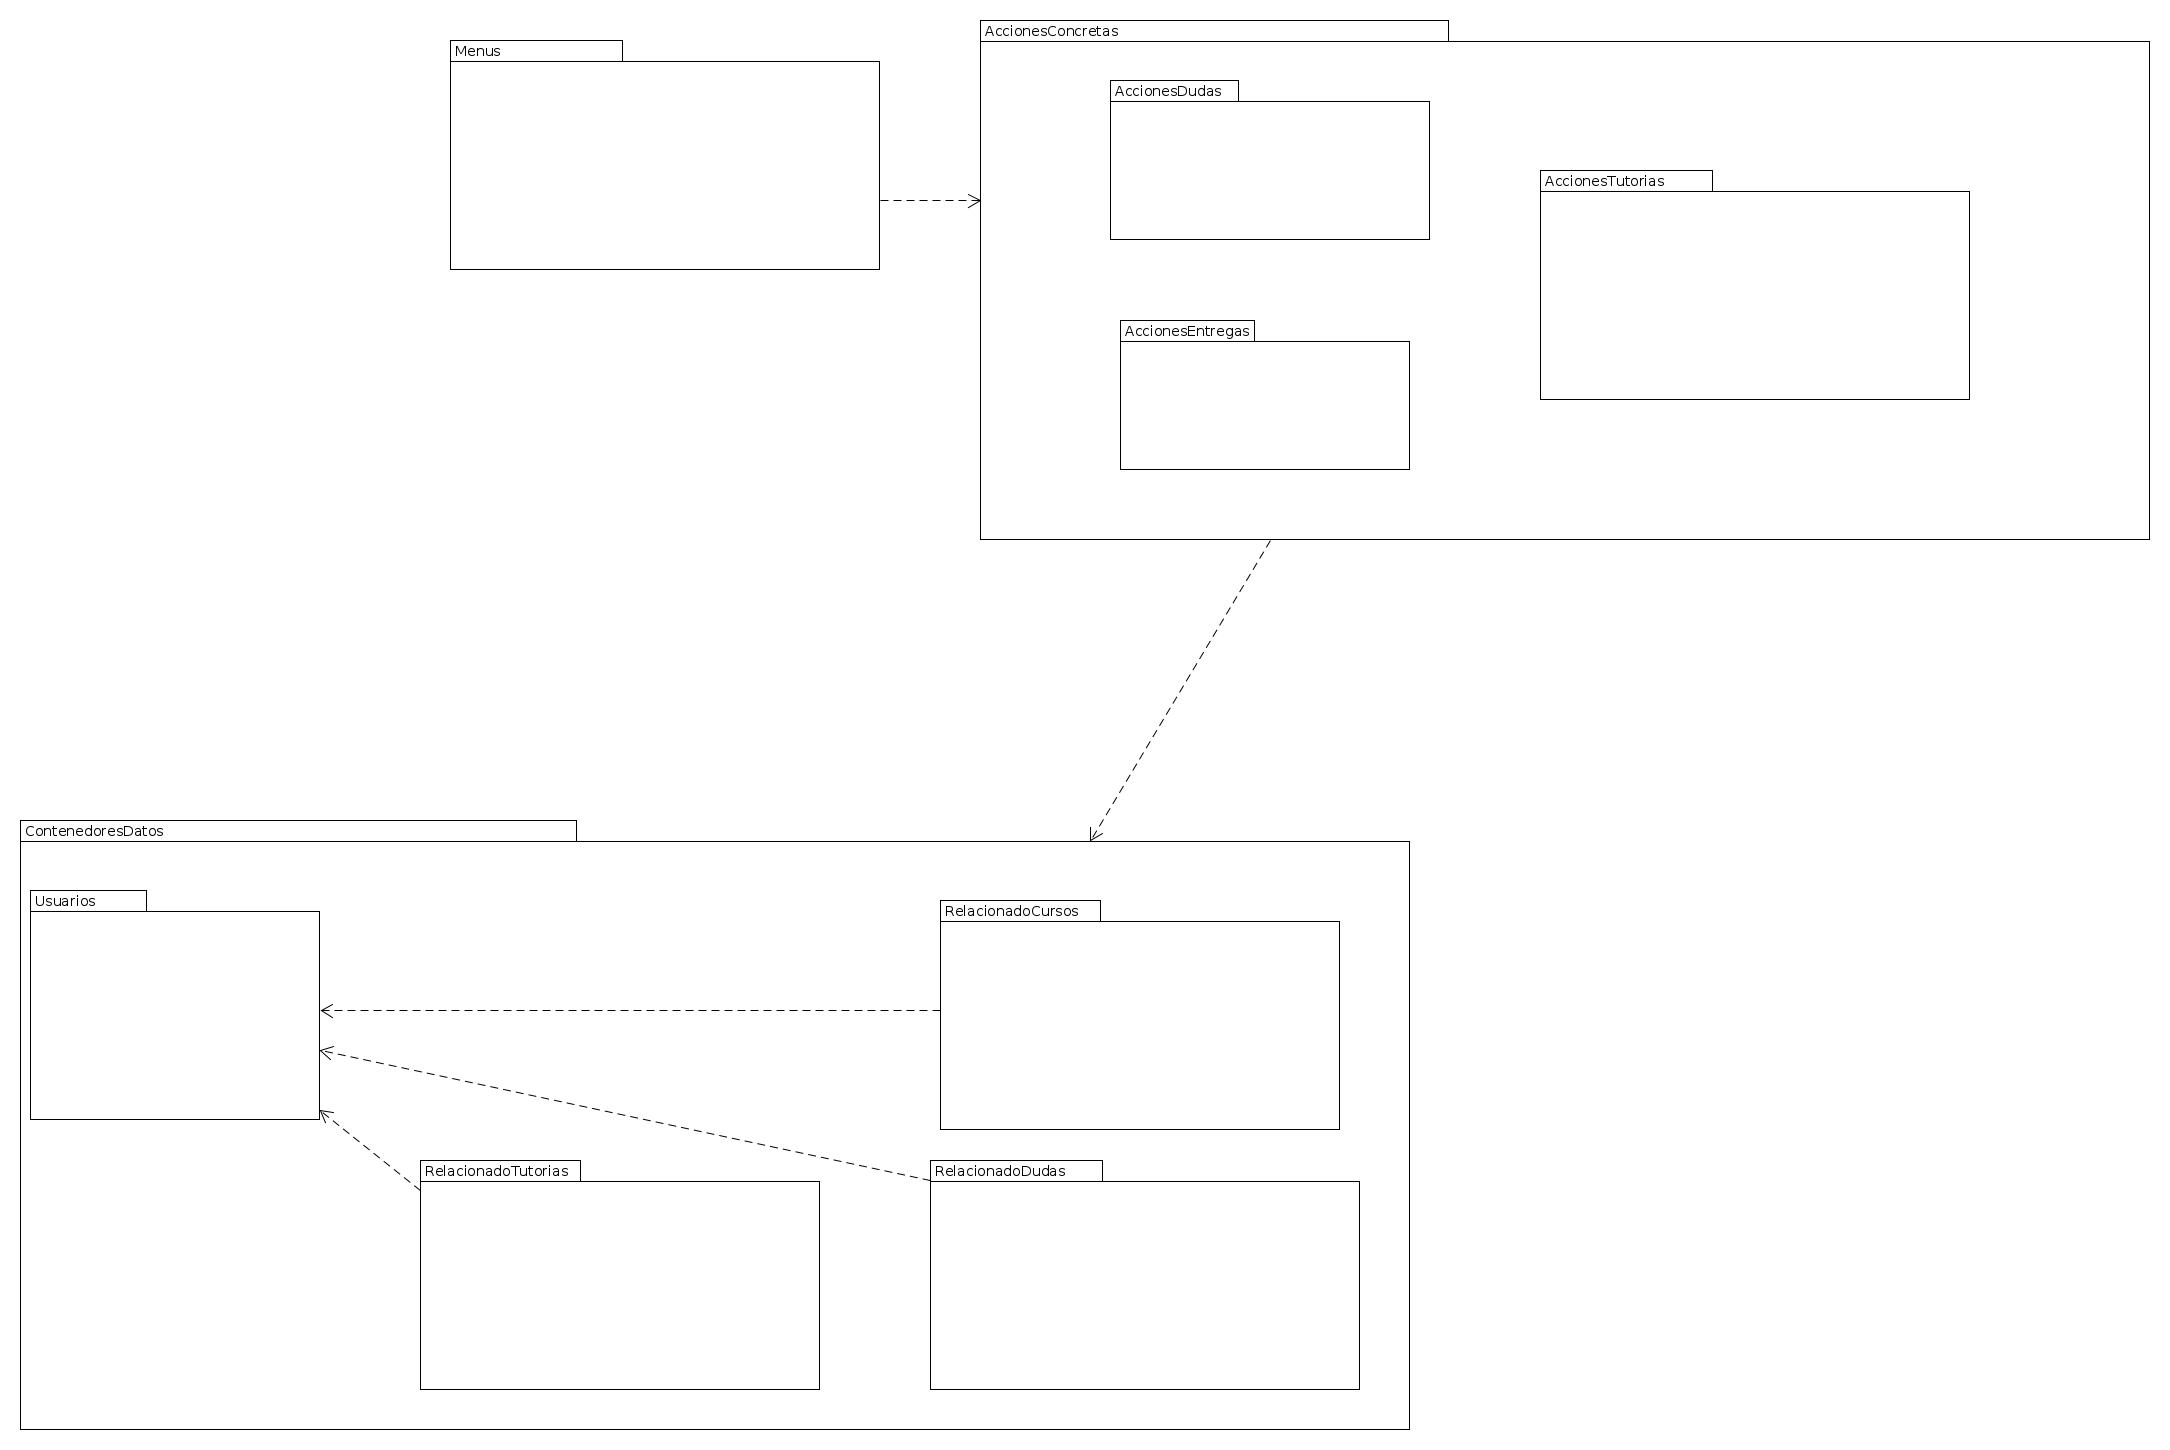
\includegraphics[scale=0.2]{imagenes/diagramas/diagrama_de_paquetes.png}  %el parámetro scale permite agrandar o achicar la imagen. En el nombre de archivo puede especificar directorios

\caption{Diagrama de paquetes del sistema}\label{figura20}
\end{figure}

    
    %%%%%%%%%%%%%%%%%%%%%%%%%%%%%%%%%%%%%%%%%
    
    \newpage
    
   \subsection{Diagramas de actividad}

A continuación mostramos los diagramas de actividad para representar el flujo de procesos contenidos en los CU.

    \begin{figure}[H] %con el [H] le obligamos a situar aquí la figura
\centering
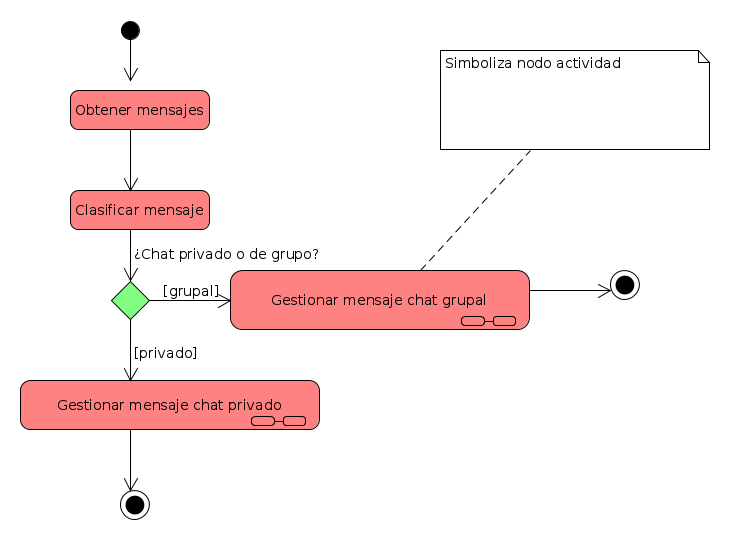
\includegraphics[scale=0.5]{imagenes/diagramas/actividad/clasificar_mensaje.png}  %el parámetro scale permite agrandar o achicar la imagen. En el nombre de archivo puede especificar directorios

\caption{Diagrama actividad CU-1.1 Clasificar mensaje}\label{figura111}
\end{figure}

    \begin{figure}[H] %con el [H] le obligamos a situar aquí la figura
\centering
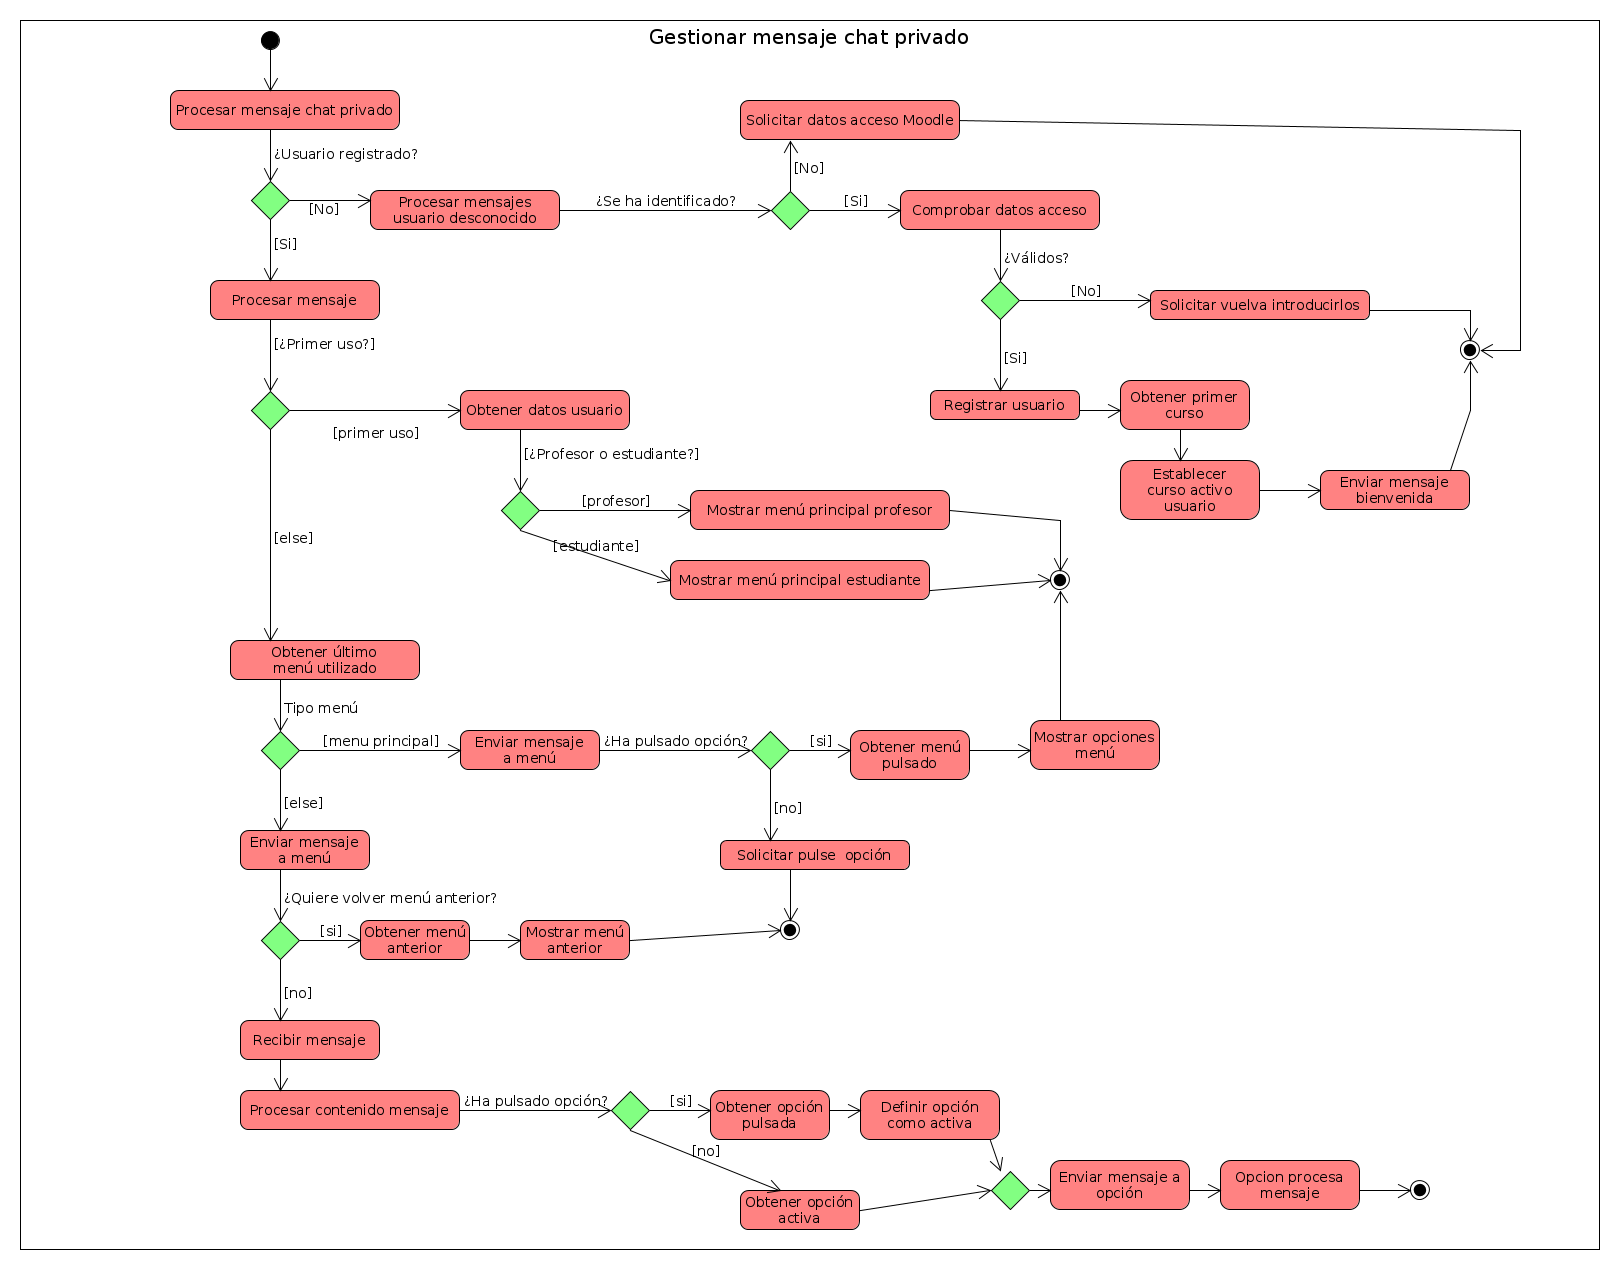
\includegraphics[scale=0.2]{imagenes/diagramas/actividad/mensaje_chat_privadoo.png}  %el parámetro scale permite agrandar o achicar la imagen. En el nombre de archivo puede especificar directorios

\caption{Diagrama actividad CU-1.2 Clasificar mensaje privado}\label{figura131}
\end{figure}
    

        \begin{figure}[H] %con el [H] le obligamos a situar aquí la figura
\centering
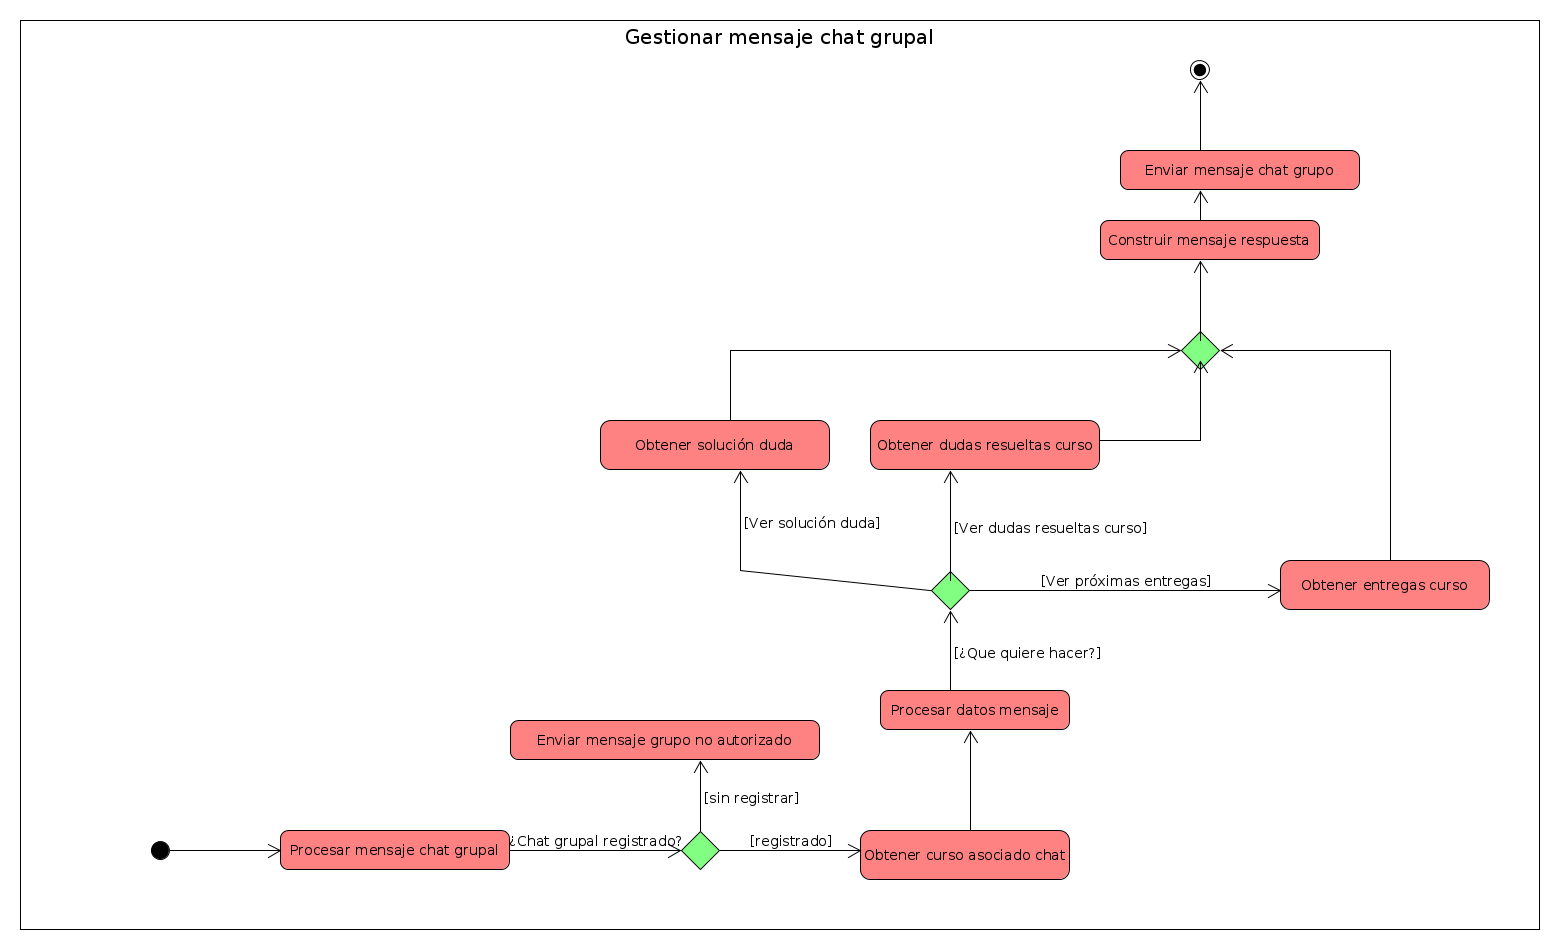
\includegraphics[scale=0.25]{imagenes/diagramas/actividad/mensaje_chat_grupall.png}  %el parámetro scale permite agrandar o achicar la imagen. En el nombre de archivo puede especificar directorios

\caption{Diagrama actividad CU-7.1, CU-7.2, CU-7.3  Mostrar solución duda, mostrar dudas resueltas y entregas por chat grupal}\label{figura141}
\end{figure}

A continucación mostramos los diagramas de actividad de los CU relacionados con las tutorías.

        \begin{figure}[H] %con el [H] le obligamos a situar aquí la figura
\centering
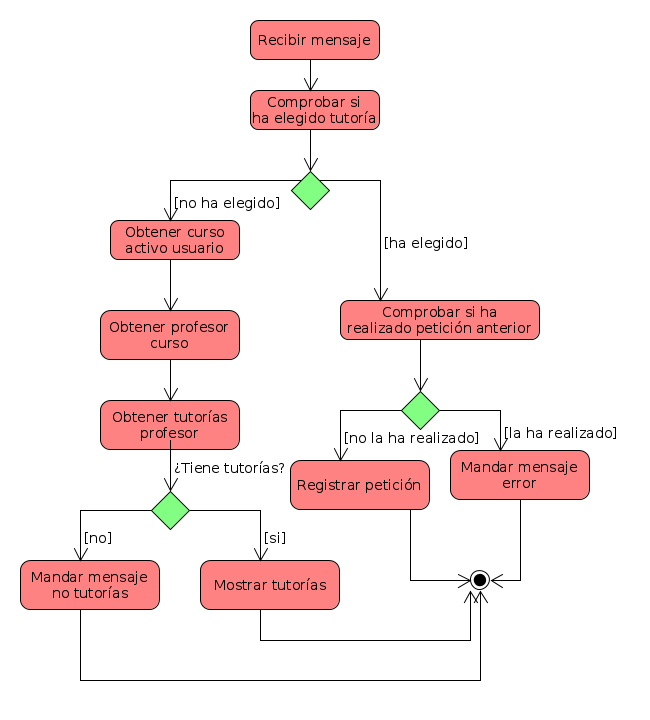
\includegraphics[scale=0.5]{imagenes/diagramas/actividad/realizar_peticon_tutoriaa.png}  %el parámetro scale permite agrandar o achicar la imagen. En el nombre de archivo puede especificar directorios

\caption{Diagrama actividad de CU-4.3 Solicitar tutoría}\label{figura143}
\end{figure}

        \begin{figure}[H] %con el [H] le obligamos a situar aquí la figura
\centering
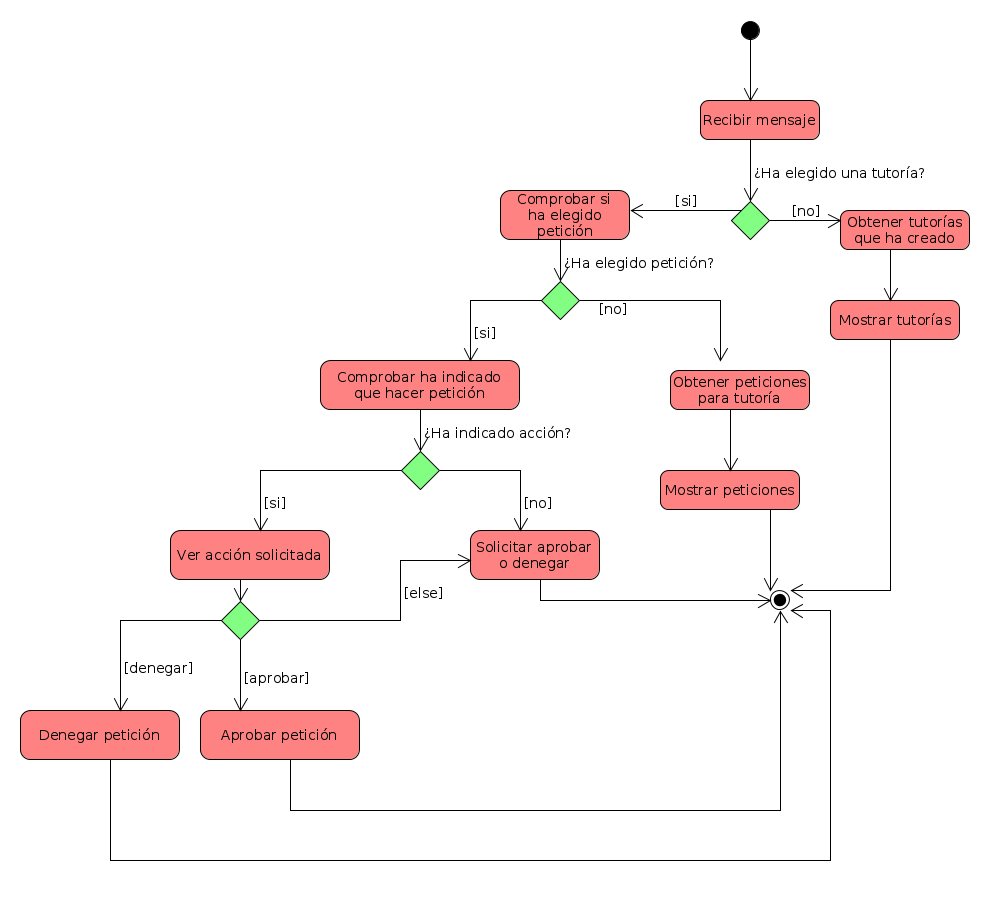
\includegraphics[scale=0.3]{imagenes/diagramas/actividad/aprobar_denegar_peticiones.png}  %el parámetro scale permite agrandar o achicar la imagen. En el nombre de archivo puede especificar directorios

\caption{Diagrama actividad conjunto de CU-4.4 Aceptar petición tutoría, CU-4.5 Denegar petición tutoría}\label{figura144}
\end{figure}

        \begin{figure}[H] %con el [H] le obligamos a situar aquí la figura
\centering
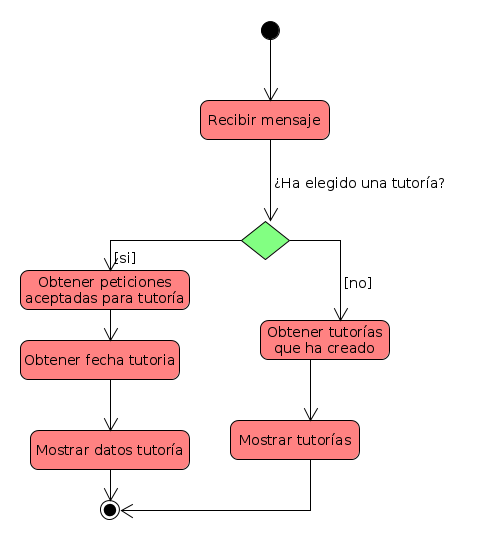
\includegraphics[scale=0.5]{imagenes/diagramas/actividad/cola_tutorias.png}  %el parámetro scale permite agrandar o achicar la imagen. En el nombre de archivo puede especificar directorios

\caption{Diagrama actividad  de CU-4.6 Ver información tutoría}\label{figura145}
\end{figure}



        \begin{figure}[H] %con el [H] le obligamos a situar aquí la figura
\centering
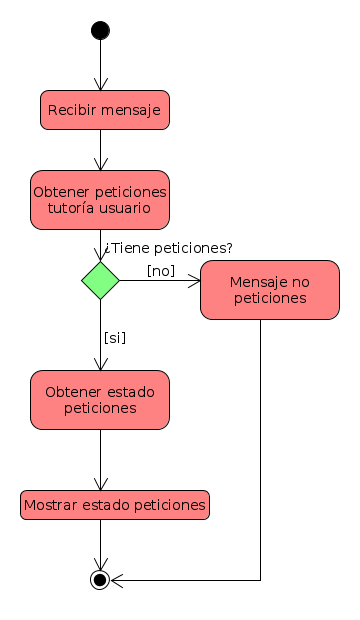
\includegraphics[scale=0.5]{imagenes/diagramas/actividad/ver_peticiones_realizadass.png}  %el parámetro scale permite agrandar o achicar la imagen. En el nombre de archivo puede especificar directorios

\caption{Diagrama actividad de CU-4.7 Ver peticiones realizadas}\label{figura147}
\end{figure}

        \begin{figure}[H] %con el [H] le obligamos a situar aquí la figura
\centering
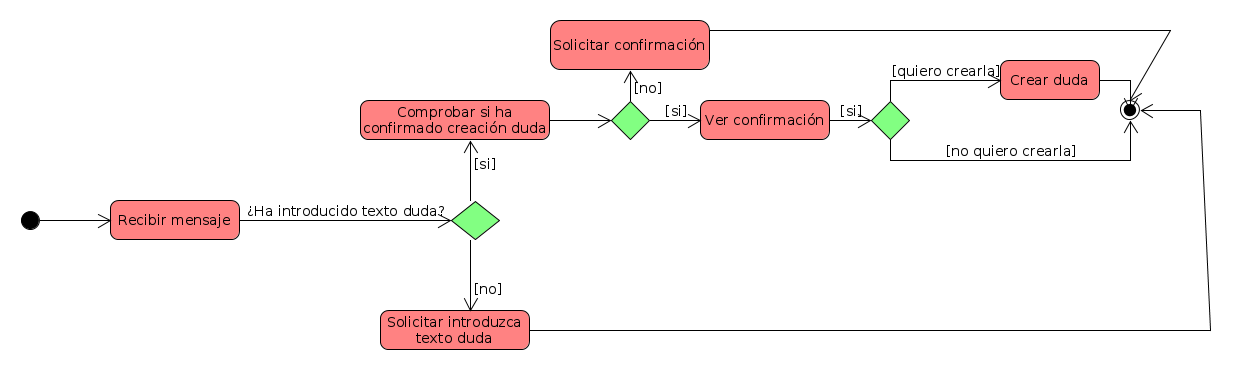
\includegraphics[scale=0.3]{imagenes/diagramas/actividad/crear_duda.png}  %el parámetro scale permite agrandar o achicar la imagen. En el nombre de archivo puede especificar directorios

\caption{Diagrama actividad de CU-5.1 Crear duda}\label{figura148}
\end{figure}

        \begin{figure}[H] %con el [H] le obligamos a situar aquí la figura
\centering
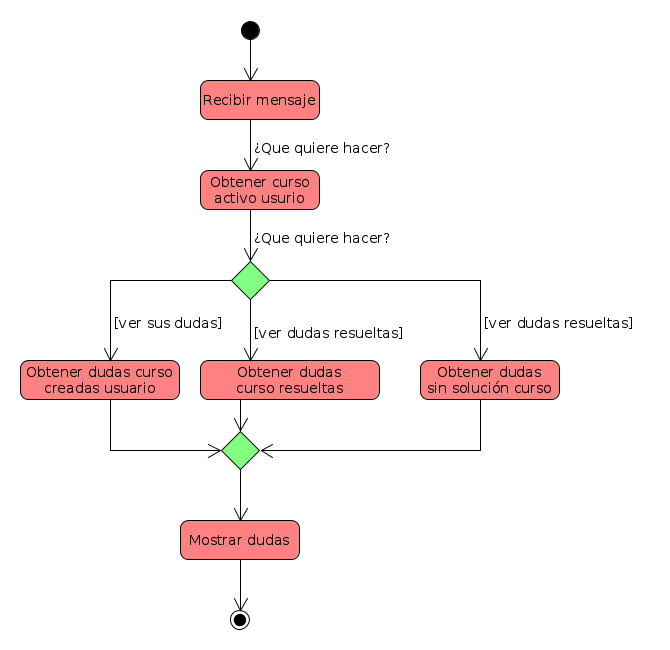
\includegraphics[scale=0.3]{imagenes/diagramas/actividad/ver_dudas_sin_con_mis.png}  %el parámetro scale permite agrandar o achicar la imagen. En el nombre de archivo puede especificar directorios

\caption{Diagrama actividad conjunto de CU-5.2 Ver dudas sin solución, CU-5.3 Ver mis dudas, CU-5.4 Ver dudas resueltas,}\label{figura1423}
\end{figure}


        \begin{figure}[H] %con el [H] le obligamos a situar aquí la figura
\centering
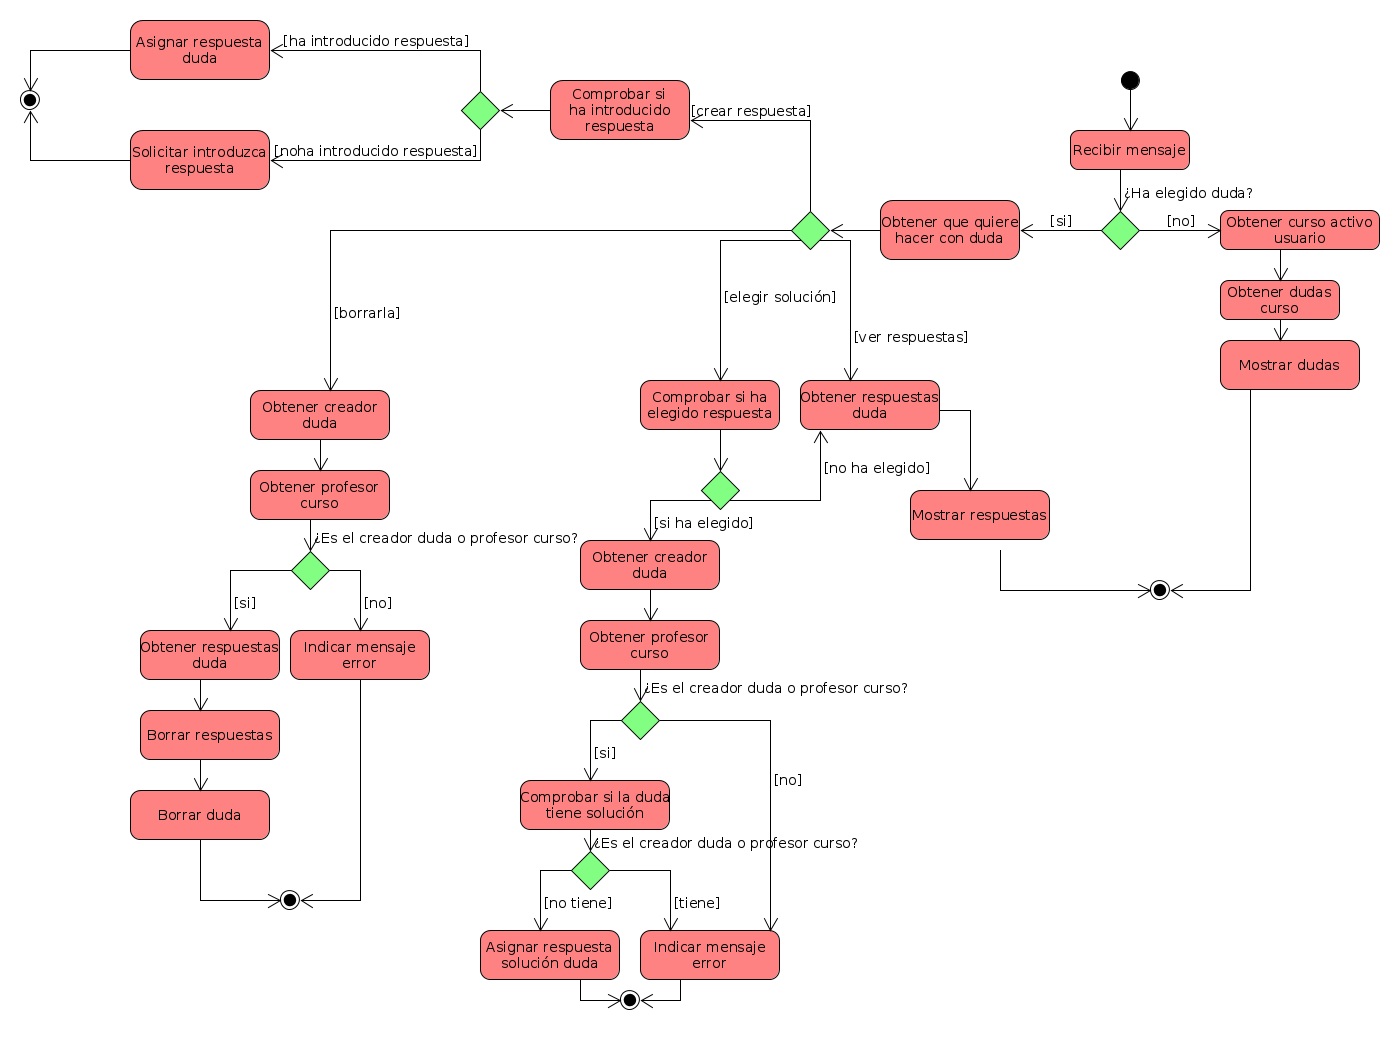
\includegraphics[scale=0.2]{imagenes/diagramas/actividad/operaciones_dudaa.png}  %el parámetro scale permite agrandar o achicar la imagen. En el nombre de archivo puede especificar directorios

\caption{Diagrama actividad conjunto de  CU-5.5 Crear respuesta a duda, CU-5.6 Ver respuesta duda, CU-5.7 Ver solución duda, CU-5.8 Borrar mi duda, CU-5.9 Elegir solución mi duda, CU-10 Borrar duda, CU-11 Elegir solución a duda}\label{figura151}
\end{figure}

        \begin{figure}[H] %con el [H] le obligamos a situar aquí la figura
\centering
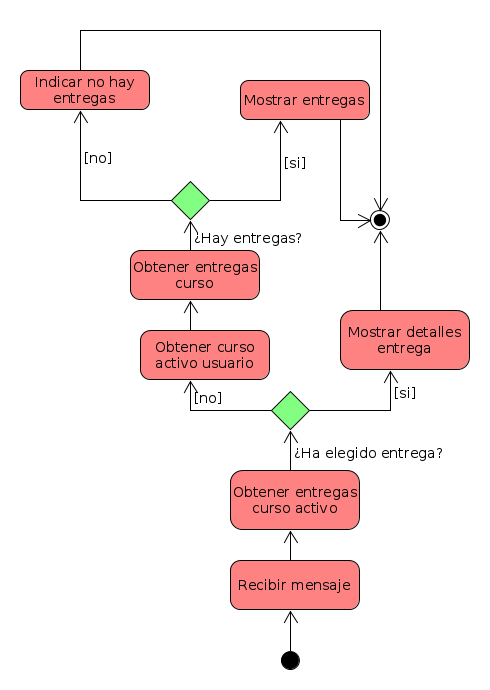
\includegraphics[scale=0.4]{imagenes/diagramas/actividad/mostrar_entregass.png}  %el parámetro scale permite agrandar o achicar la imagen. En el nombre de archivo puede especificar directorios

\caption{Diagrama actividad CU-6.1 Ver entregas}\label{figura153}
\end{figure}

        \begin{figure}[H] %con el [H] le obligamos a situar aquí la figura
\centering
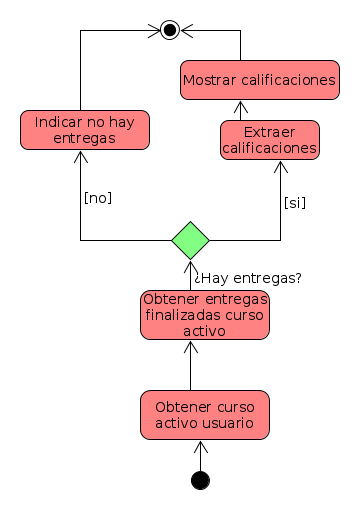
\includegraphics[scale=0.4]{imagenes/diagramas/actividad/mostrar_calificaciones.png}  %el parámetro scale permite agrandar o achicar la imagen. En el nombre de archivo puede especificar directorios

\caption{Diagrama actividad CU-6.2 Mostrar calificaciones}\label{figura152}
\end{figure}



    
%

\chapter{}

\section{Analisis de los requisitos}
    
    \subsection{Modelo conceptual}

A continuación podemos ver los principales conceptos que comprende el sistema y cómo se relacionan. De la interfaz y sus conceptos hablaremos en el diseño de la interfaz.


 \begin{figure}[H] %con el [H] le obligamos a situar aquí la figura
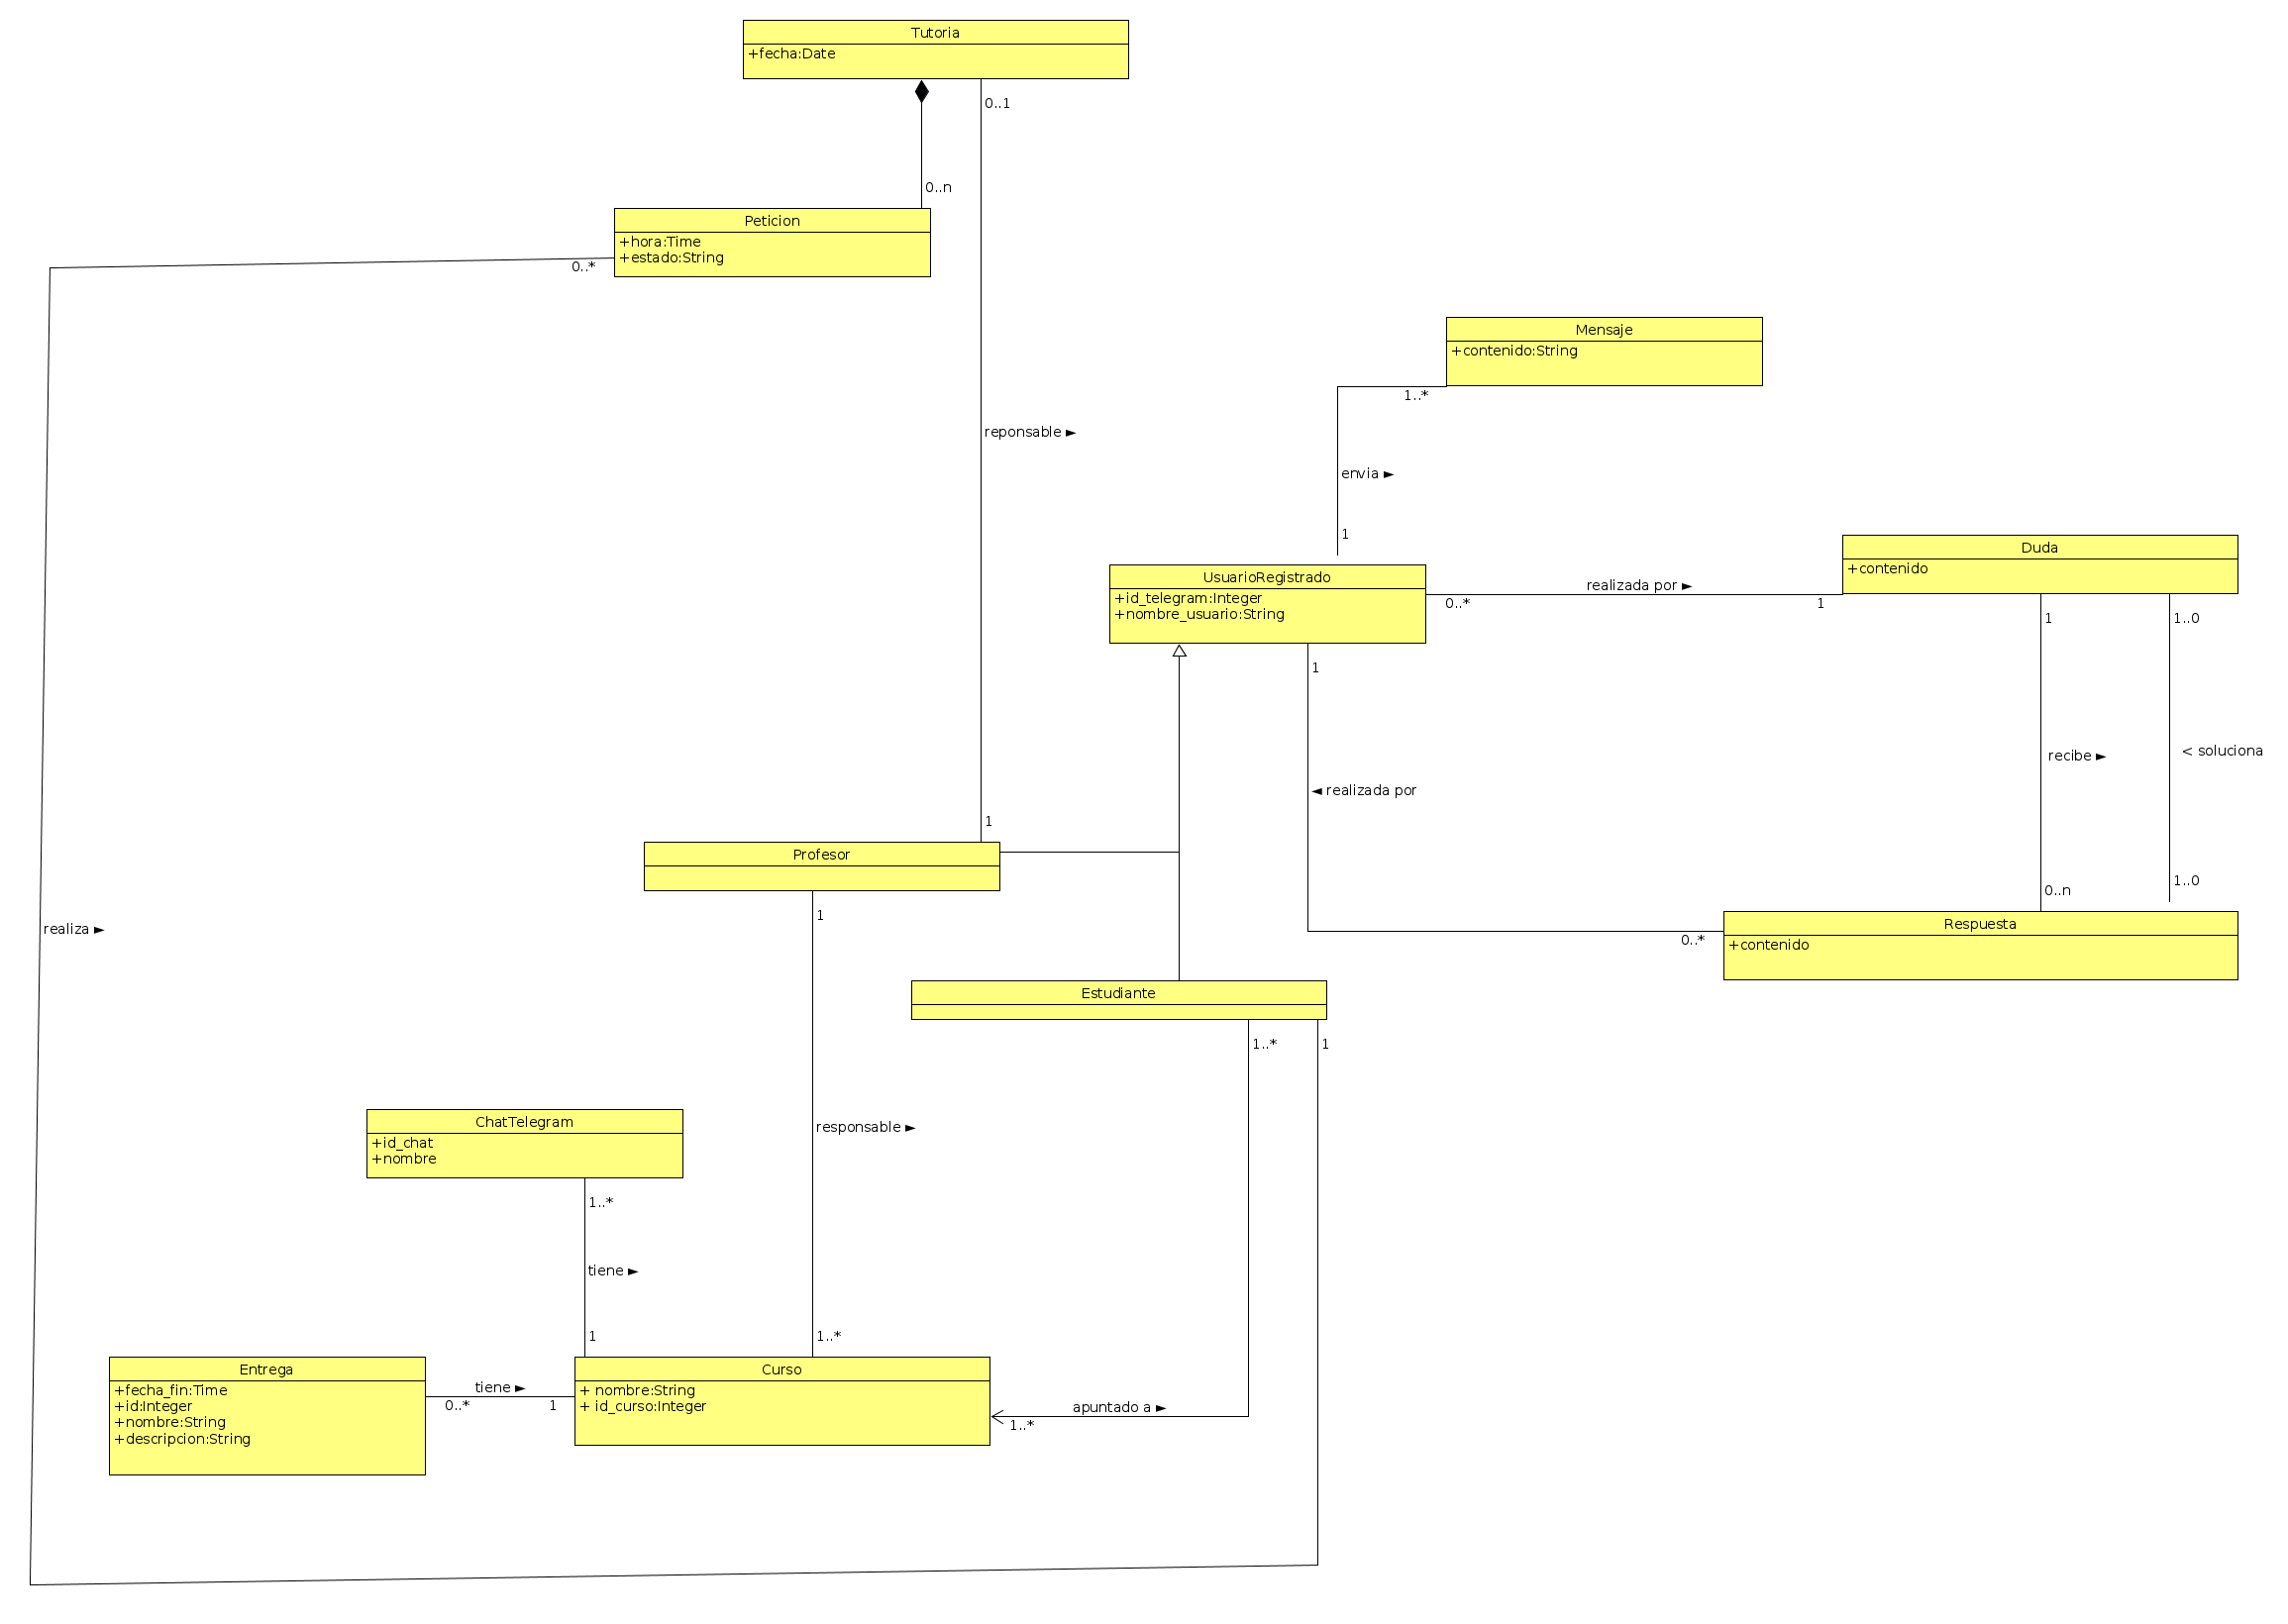
\includegraphics[width=1.1\textwidth, right]{imagenes/diagramas/diagrama_conceptual.png}  %el parámetro scale permite agrandar o achicar la imagen. En el nombre de archivo puede especificar directorios
\caption{Diagrama conceptual del sistema}\label{figura197}
\end{figure}


Presenta cierto parecido con el diagrama de casos de uso: profesor y estudiante heredan de usuario registrado que tienen relación con las dudas, profesor responsable de las tutorías y el estudiante realiza peticiones a éstas.

\subsection{Diagramas secuencia}

La meta buscada en esta sección es mostrar las interacciones entre los objetos que provoca la realización de algunos de los CUs más importantes por parte de los actores. Ahora mismo hay una clase \enquote*{pradobot} que hace de mediadora entre el usuario y el resto de clases del sistema. Esta clase dirime qué es lo que quiere el usuario y lleva a cabo las interacciones necesarias con el resto de clases para cumplir el objetivo del usuario. Todas estas operaciones exigidas por el usuario se traducirán en interfaces cuyo diseño se tratará en la sección de diseño interacción usuario.


\begin{figure}[H] %con el [H] le obligamos a situar aquí la figura
\centering
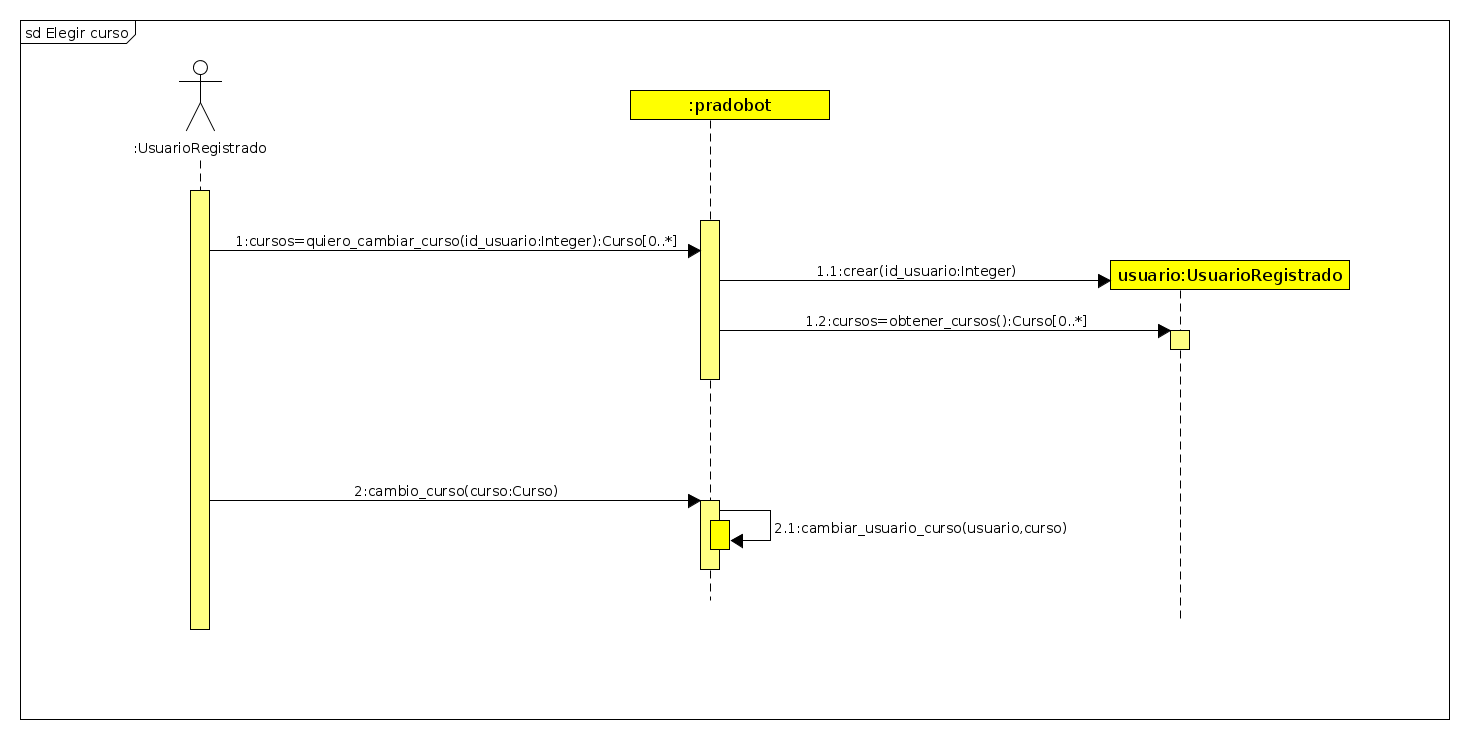
\includegraphics[scale=0.3]{imagenes/diagramas/secuencia/analisis/elegir_curso.png}  %el parámetro scale permite agrandar o achicar la imagen. En el nombre de archivo puede especificar directorios

\caption{DS: Cambiar curso (CU-1.4) }\label{figura62}

\end{figure}

\begin{figure}[H] %con el [H] le obligamos a situar aquí la figura
\centering
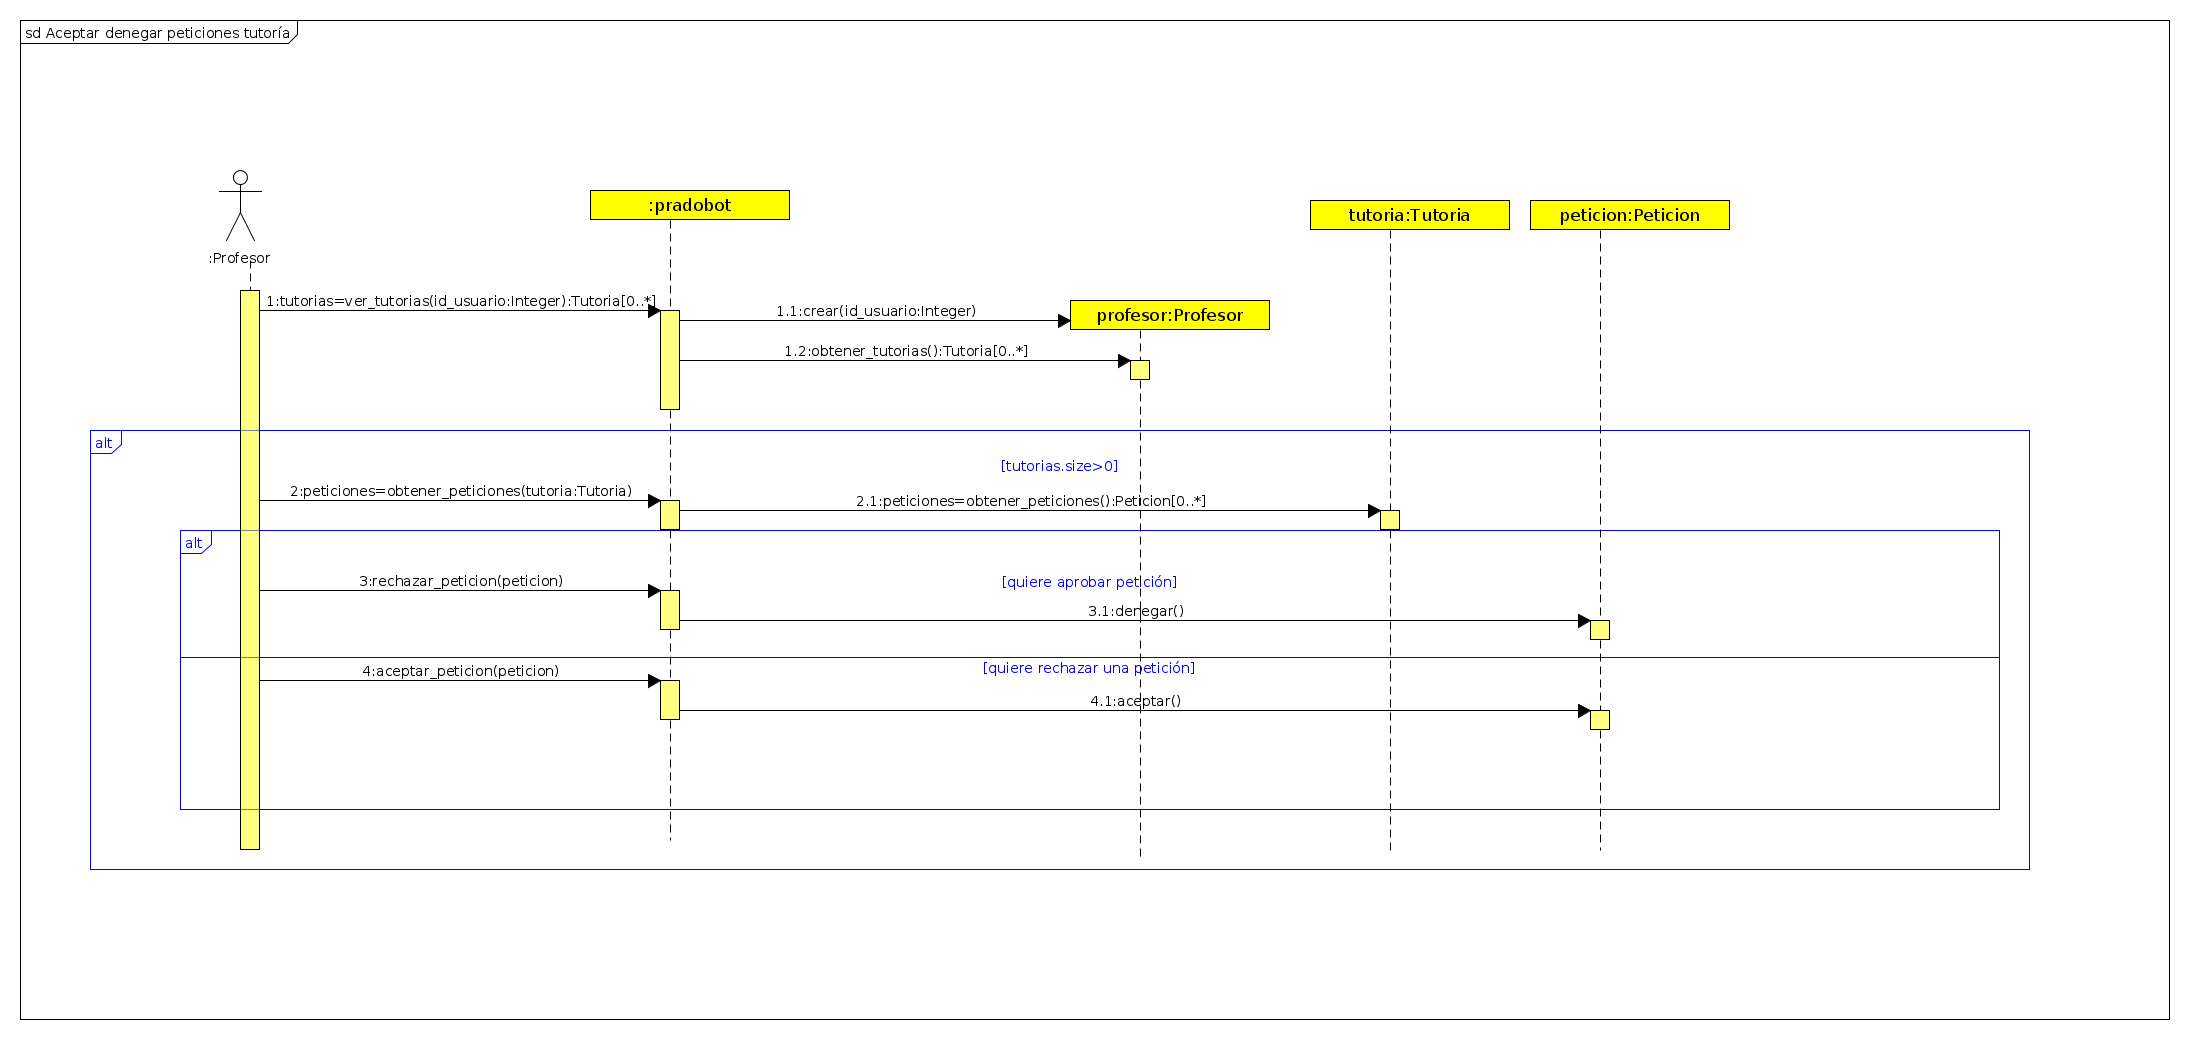
\includegraphics[scale=0.2]{imagenes/diagramas/secuencia/analisis/aceptar_denegar_peticion.png}  %el parámetro scale permite agrandar o achicar la imagen. En el nombre de archivo puede especificar directorios

\caption{DS: Aceptar denegar peticiones (CU-4.4, CU-4.5) }\label{figura72}

\end{figure}

\begin{figure}[H] %con el [H] le obligamos a situar aquí la figura
\centering
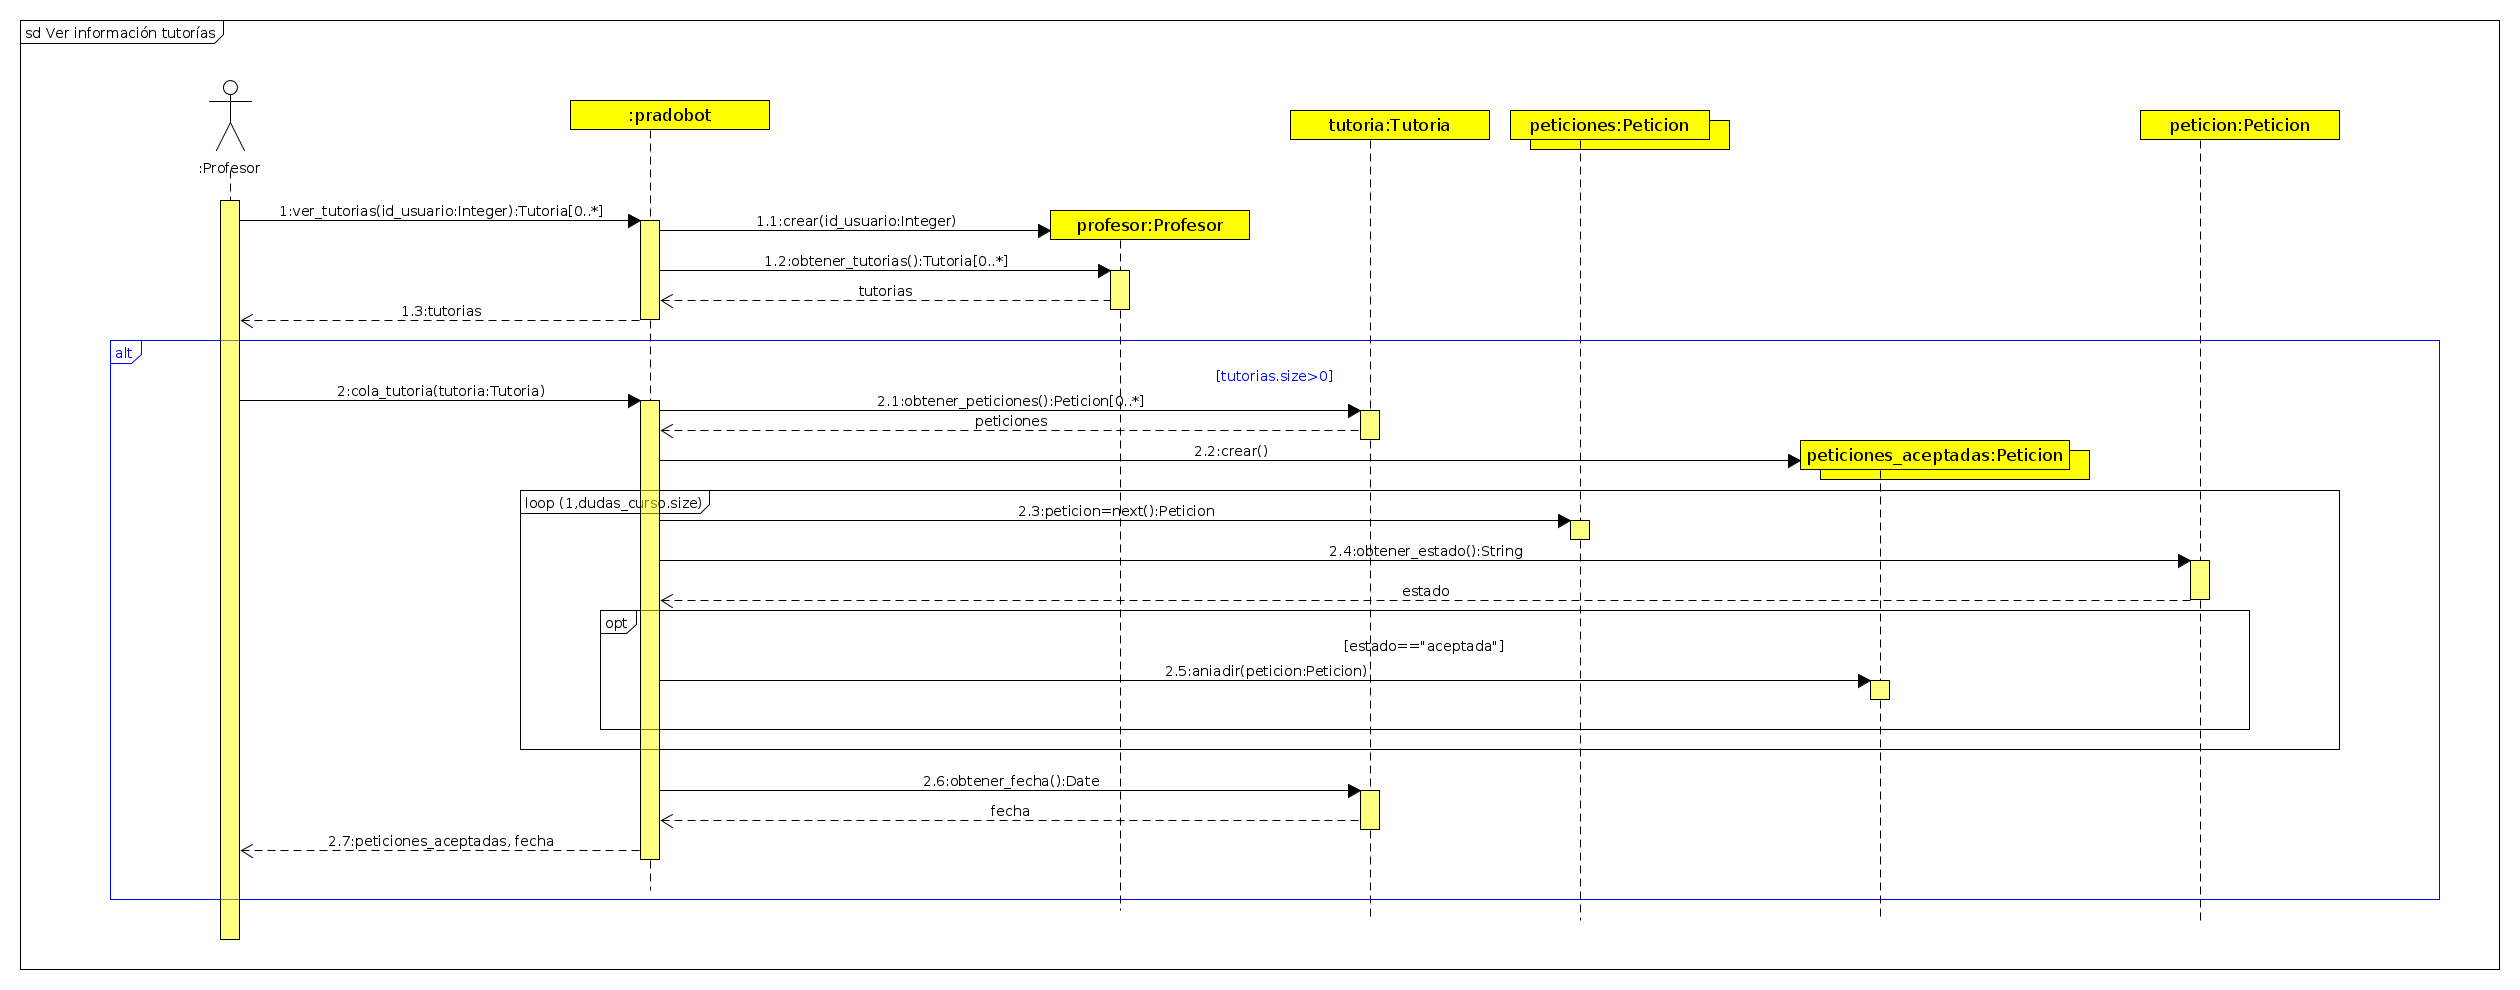
\includegraphics[width=1.3\textwidth]{imagenes/diagramas/secuencia/analisis/ver_informacion_tutoria.png}  %el parámetro scale permite agrandar o achicar la imagen. En el nombre de archivo puede especificar directorios

\caption{DS: Ver información tutoria (CU-4.6) }\label{figura77}

\end{figure}

\begin{figure}[H] %con el [H] le obligamos a situar aquí la figura
\centering
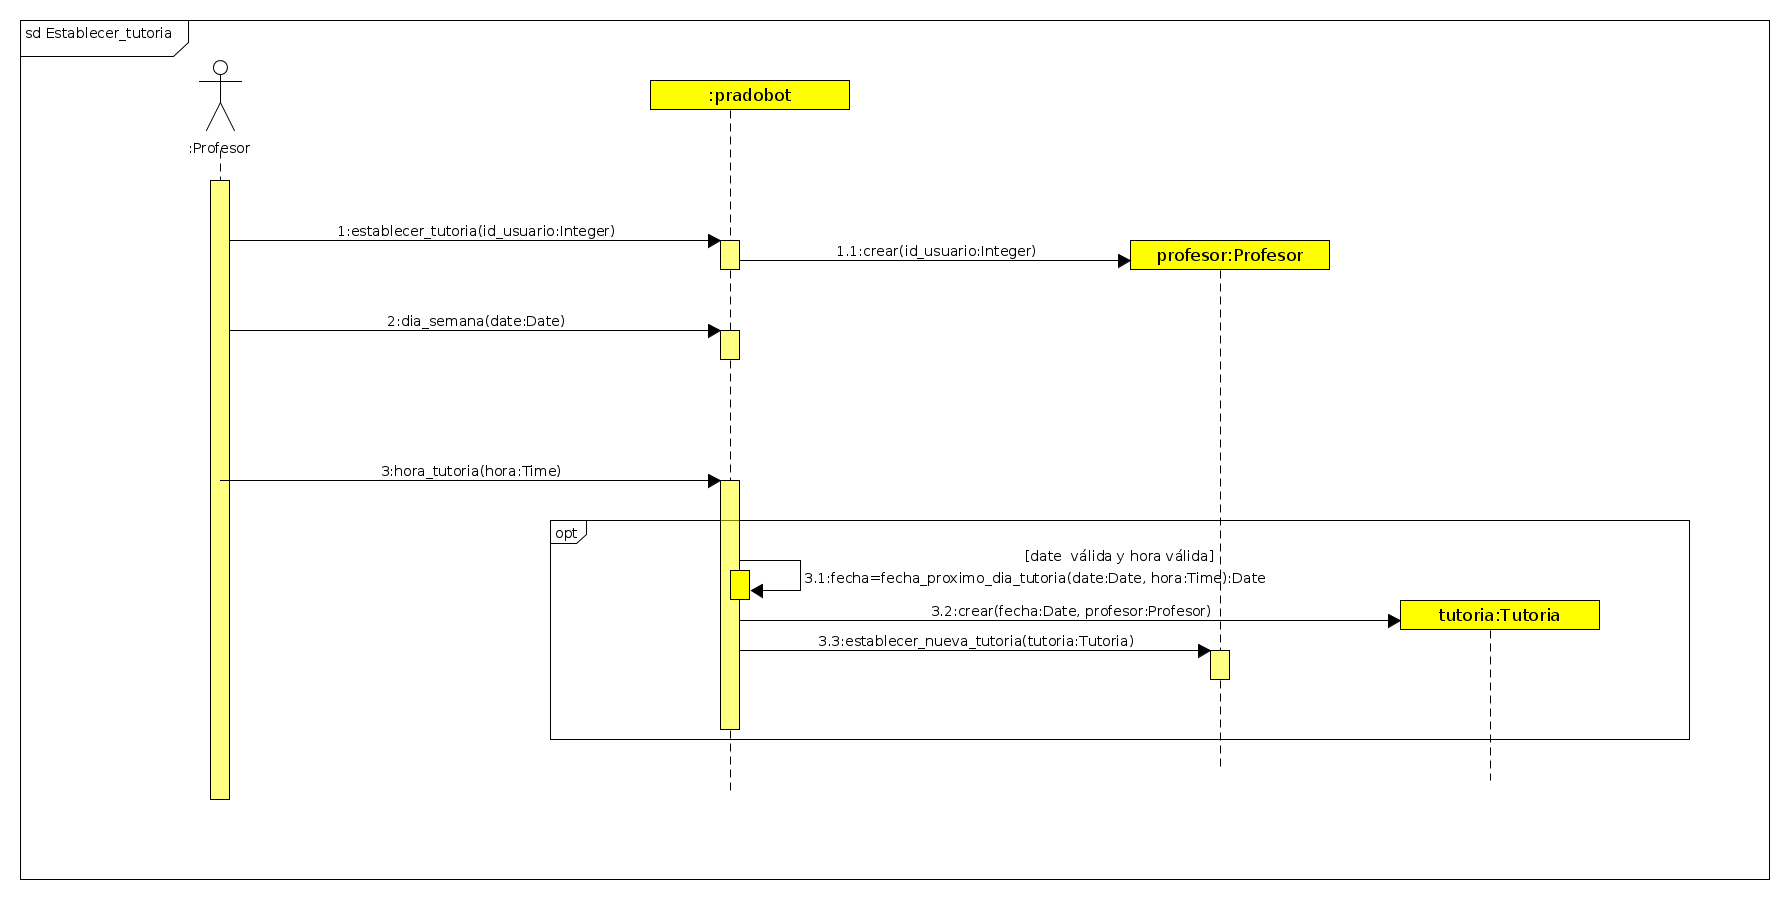
\includegraphics[width=1.2\textwidth, right]{imagenes/diagramas/secuencia/analisis/establecer_tutoria.png}  %el parámetro scale permite agrandar o achicar la imagen. En el nombre de archivo puede especificar directorios

\caption{DS: Establecer tutoría (CU-4.1) }\label{figura211}

\end{figure}

\begin{figure}[H] %con el [H] le obligamos a situar aquí la figura
\centering
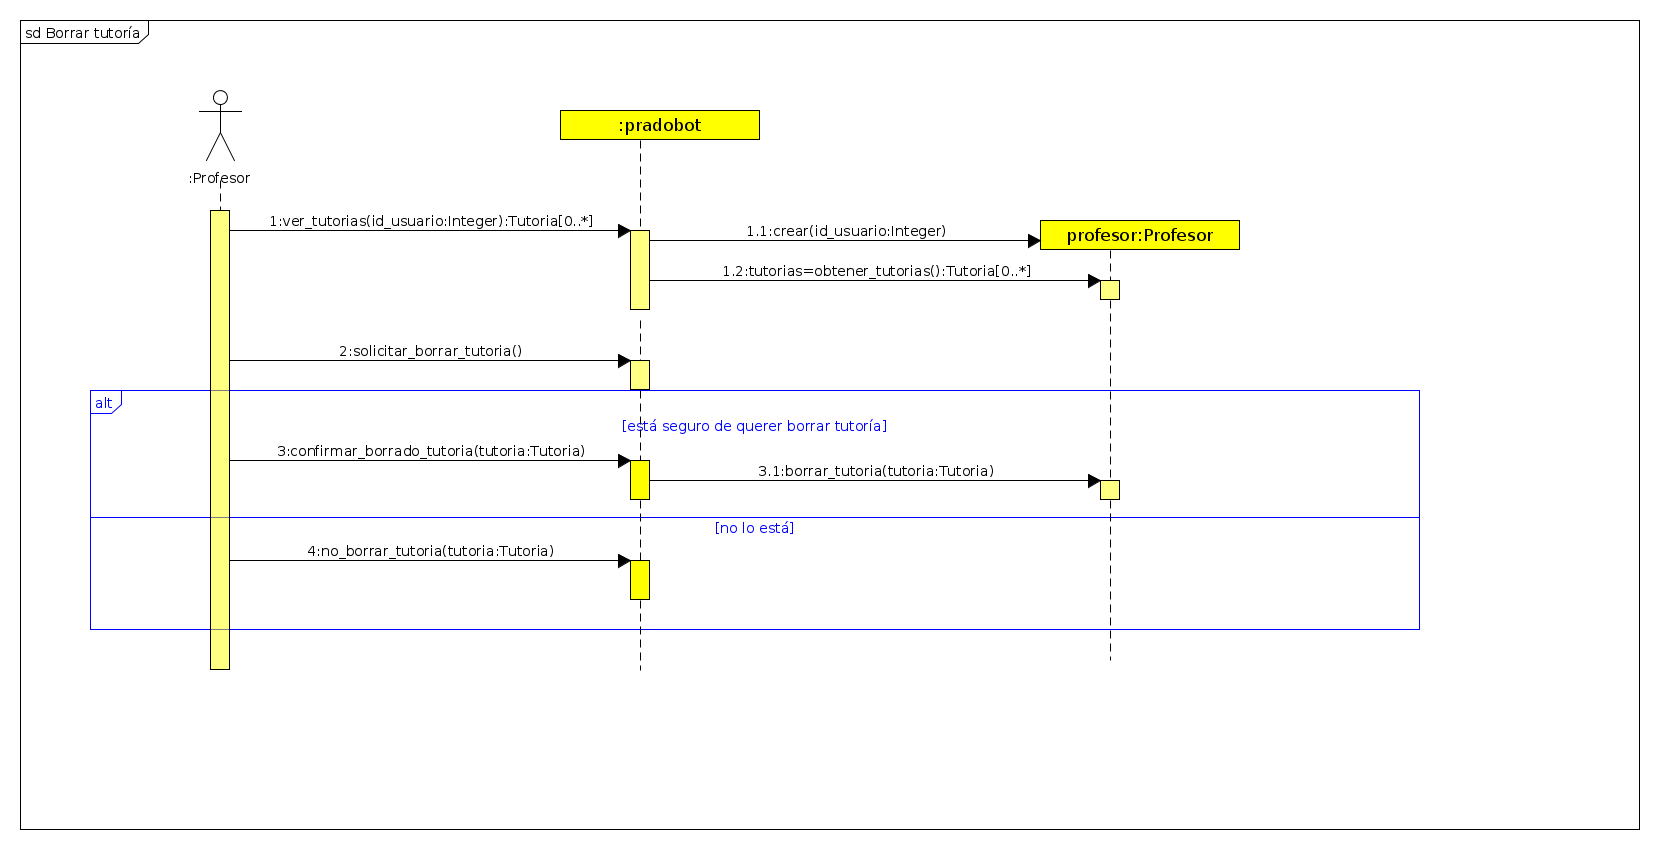
\includegraphics[scale=0.27]{imagenes/diagramas/secuencia/analisis/borrar_tutoria.png}  %el parámetro scale permite agrandar o achicar la imagen. En el nombre de archivo puede especificar directorios

\caption{DS: Borrar tutoría (CU-4.2) }\label{figura78}

\end{figure}

\begin{figure}[H] %con el [H] le obligamos a situar aquí la figura
\centering
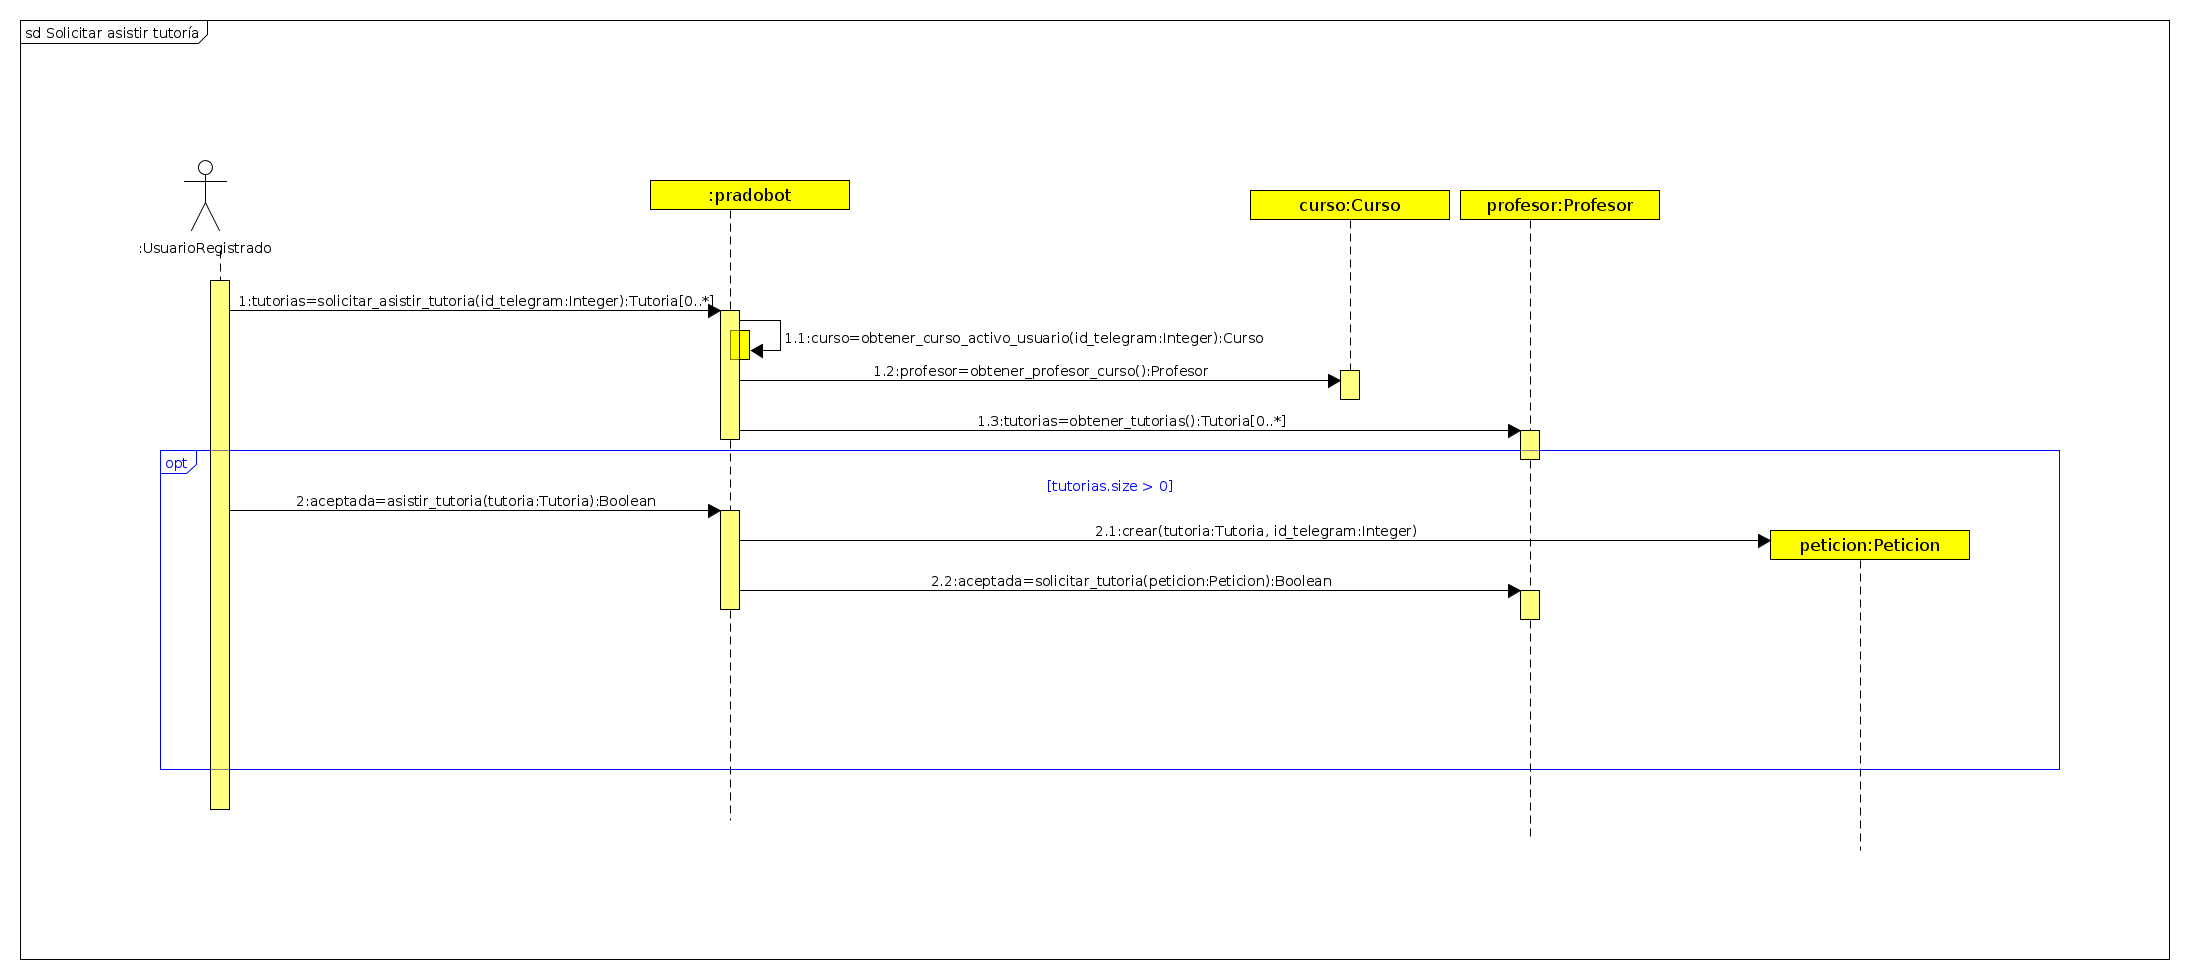
\includegraphics[scale=0.22]{imagenes/diagramas/secuencia/analisis/asistir_tutoria.png}  %el parámetro scale permite agrandar o achicar la imagen. En el nombre de archivo puede especificar directorios

\caption{DS: Solicitar asistir tutoría (CU-4.3) }\label{figura79}

\end{figure}

\begin{figure}[H] %con el [H] le obligamos a situar aquí la figura
\centering
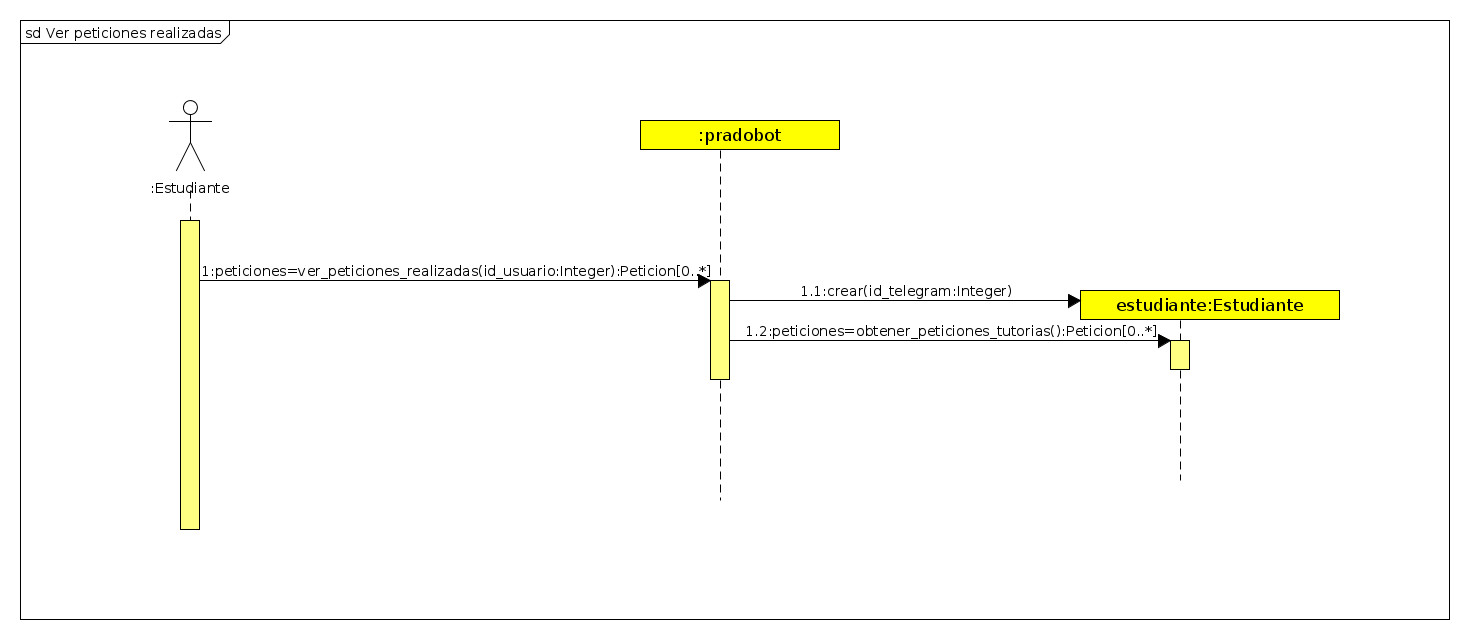
\includegraphics[scale=0.3]{imagenes/diagramas/secuencia/analisis/ver_peticiones_realizadas.png}  %el parámetro scale permite agrandar o achicar la imagen. En el nombre de archivo puede especificar directorios

\caption{DS: Ver solicitudes realizadas (CU-4.7) }\label{figura80}

\end{figure}


\begin{figure}[H] %con el [H] le obligamos a situar aquí la figura
\centering
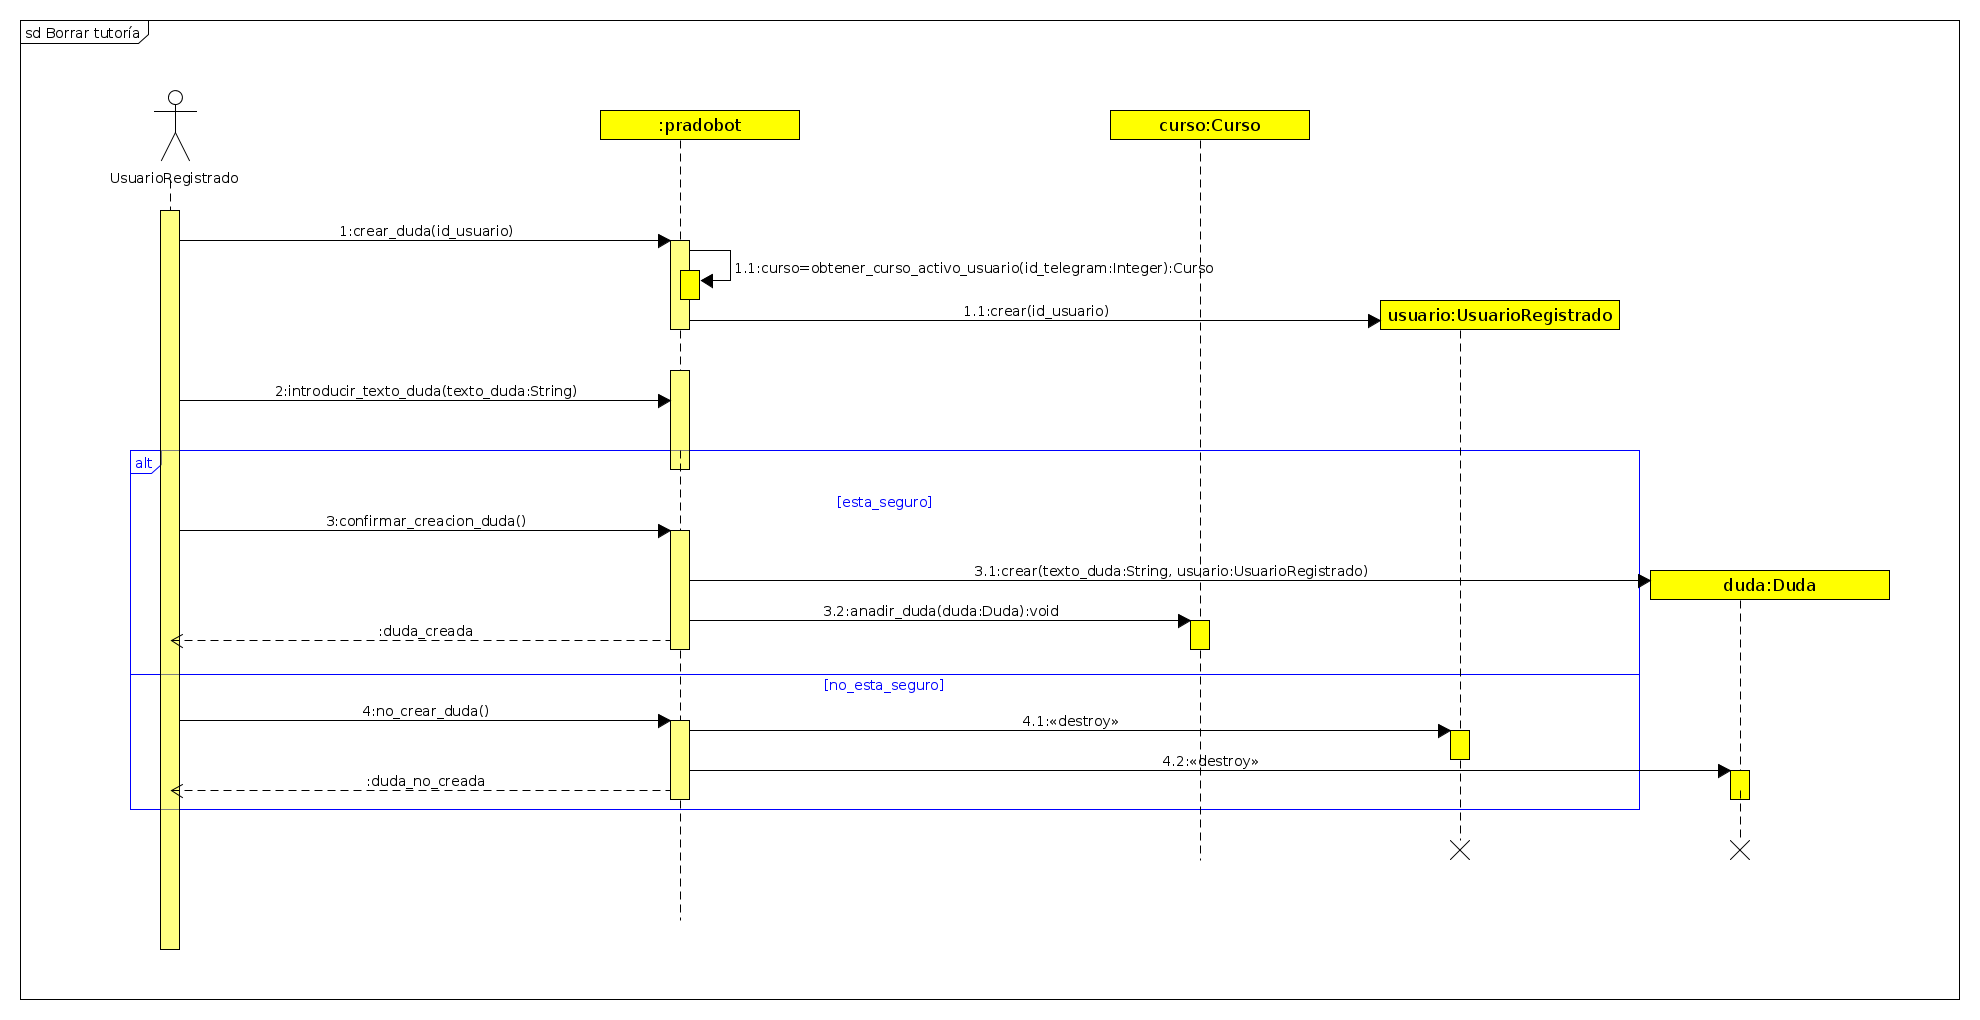
\includegraphics[scale=0.22]{imagenes/diagramas/secuencia/analisis/crear_duda.png}  %el parámetro scale permite agrandar o achicar la imagen. En el nombre de archivo puede especificar directorios

\caption{DS: Crear duda (CU-5.1) }\label{figura81}

\end{figure}

\begin{figure}[H] %con el [H] le obligamos a situar aquí la figura
\centering
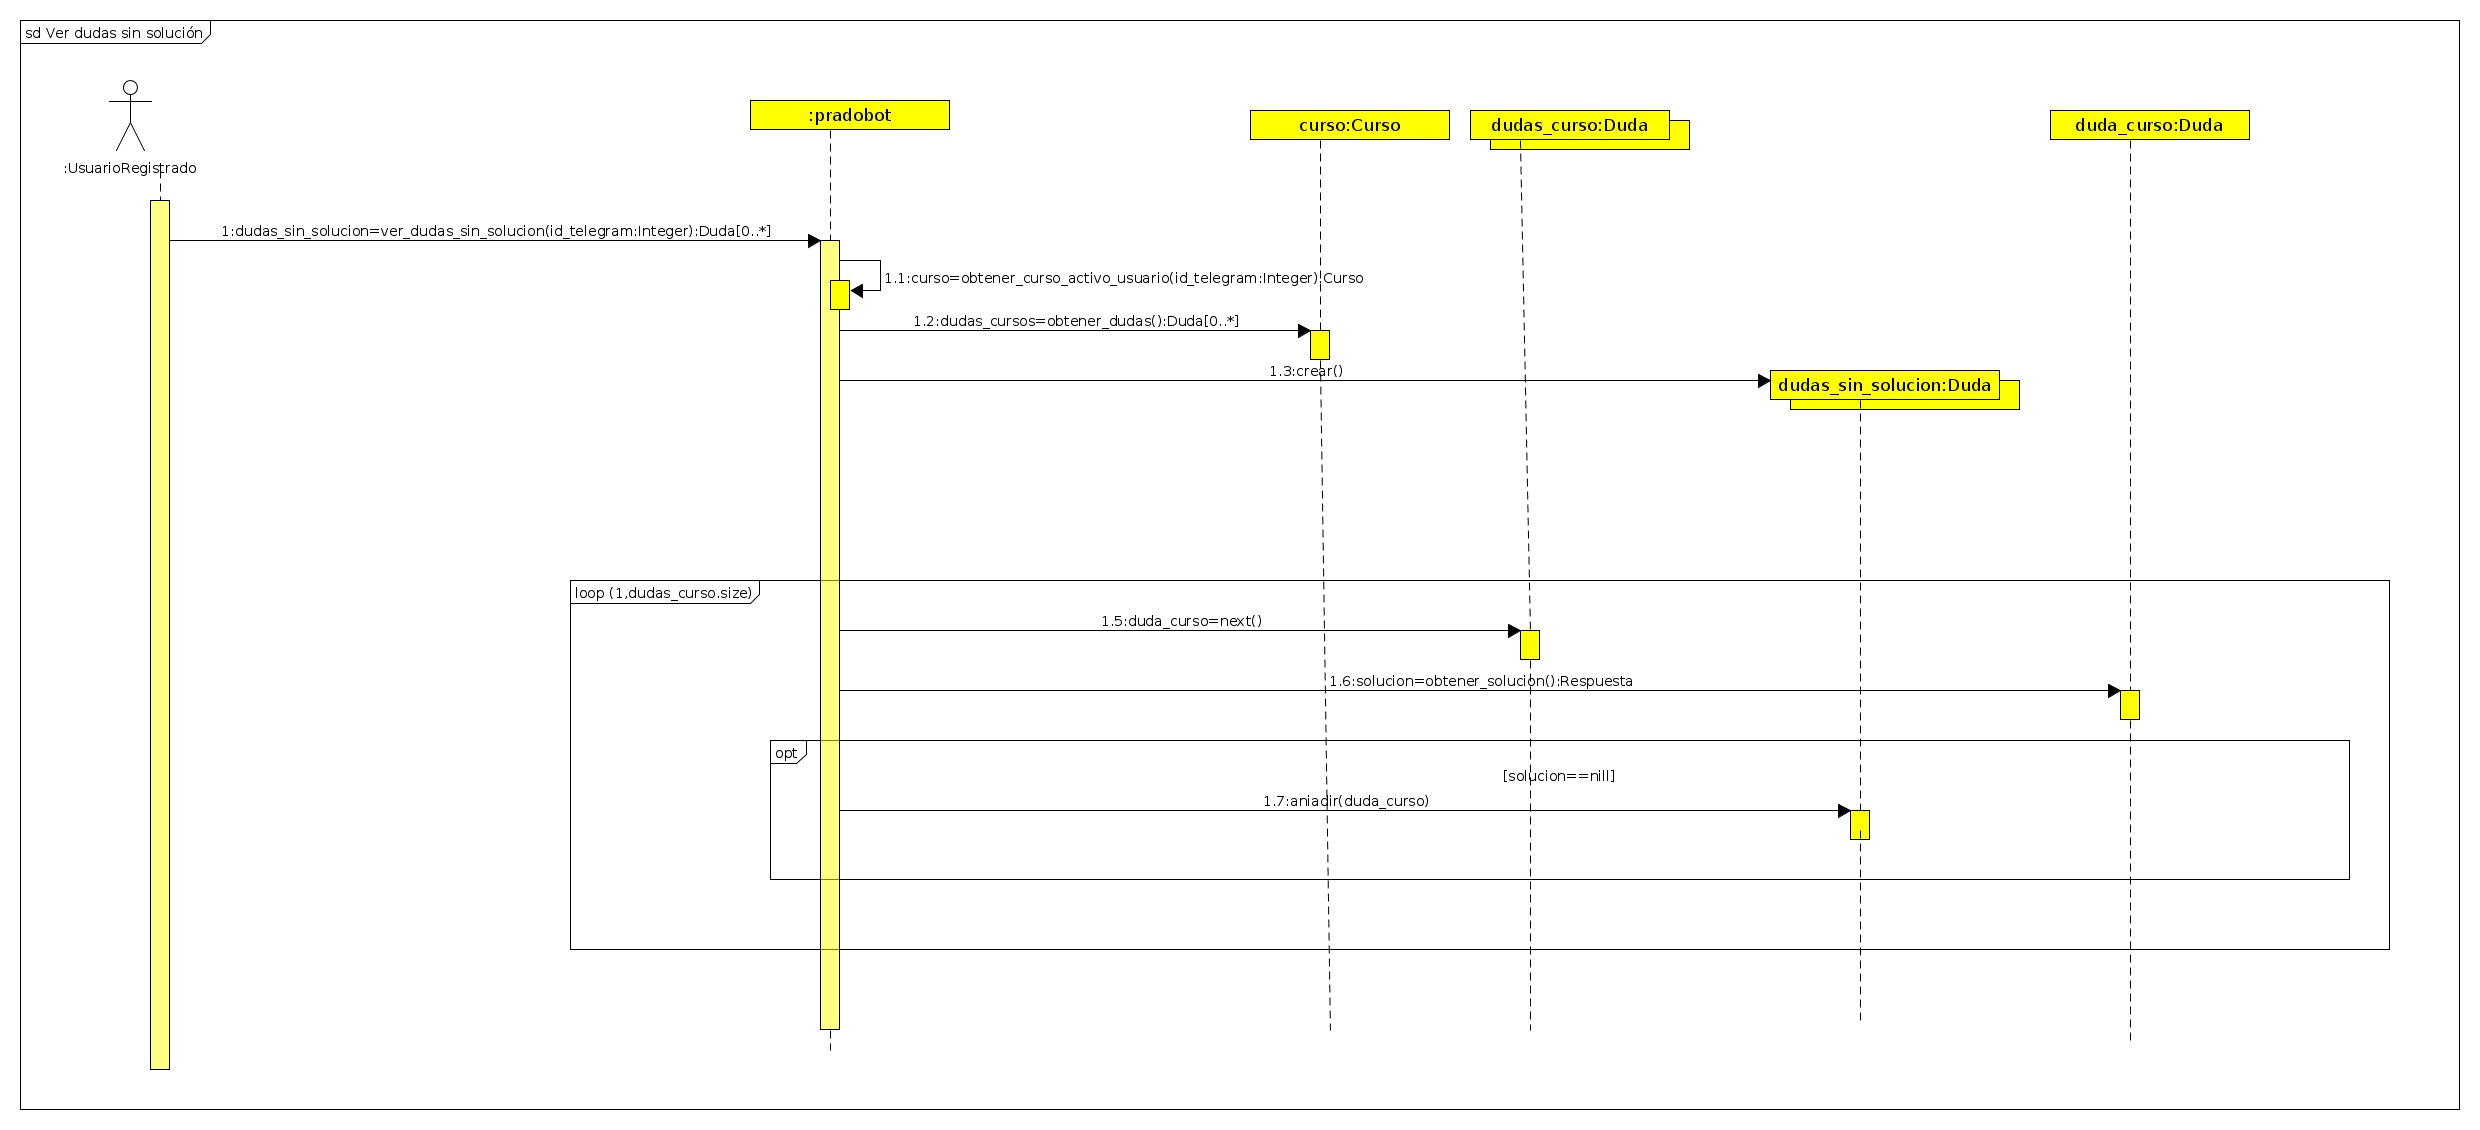
\includegraphics[scale=0.17]{imagenes/diagramas/secuencia/analisis/ver_dudas_sin_solucion.png}  %el parámetro scale permite agrandar o achicar la imagen. En el nombre de archivo puede especificar directorios

\caption{DS: Ver dudas sin solución (CU-5.2) }\label{figura83}

\end{figure}

\begin{figure}[H] %con el [H] le obligamos a situar aquí la figura
\centering
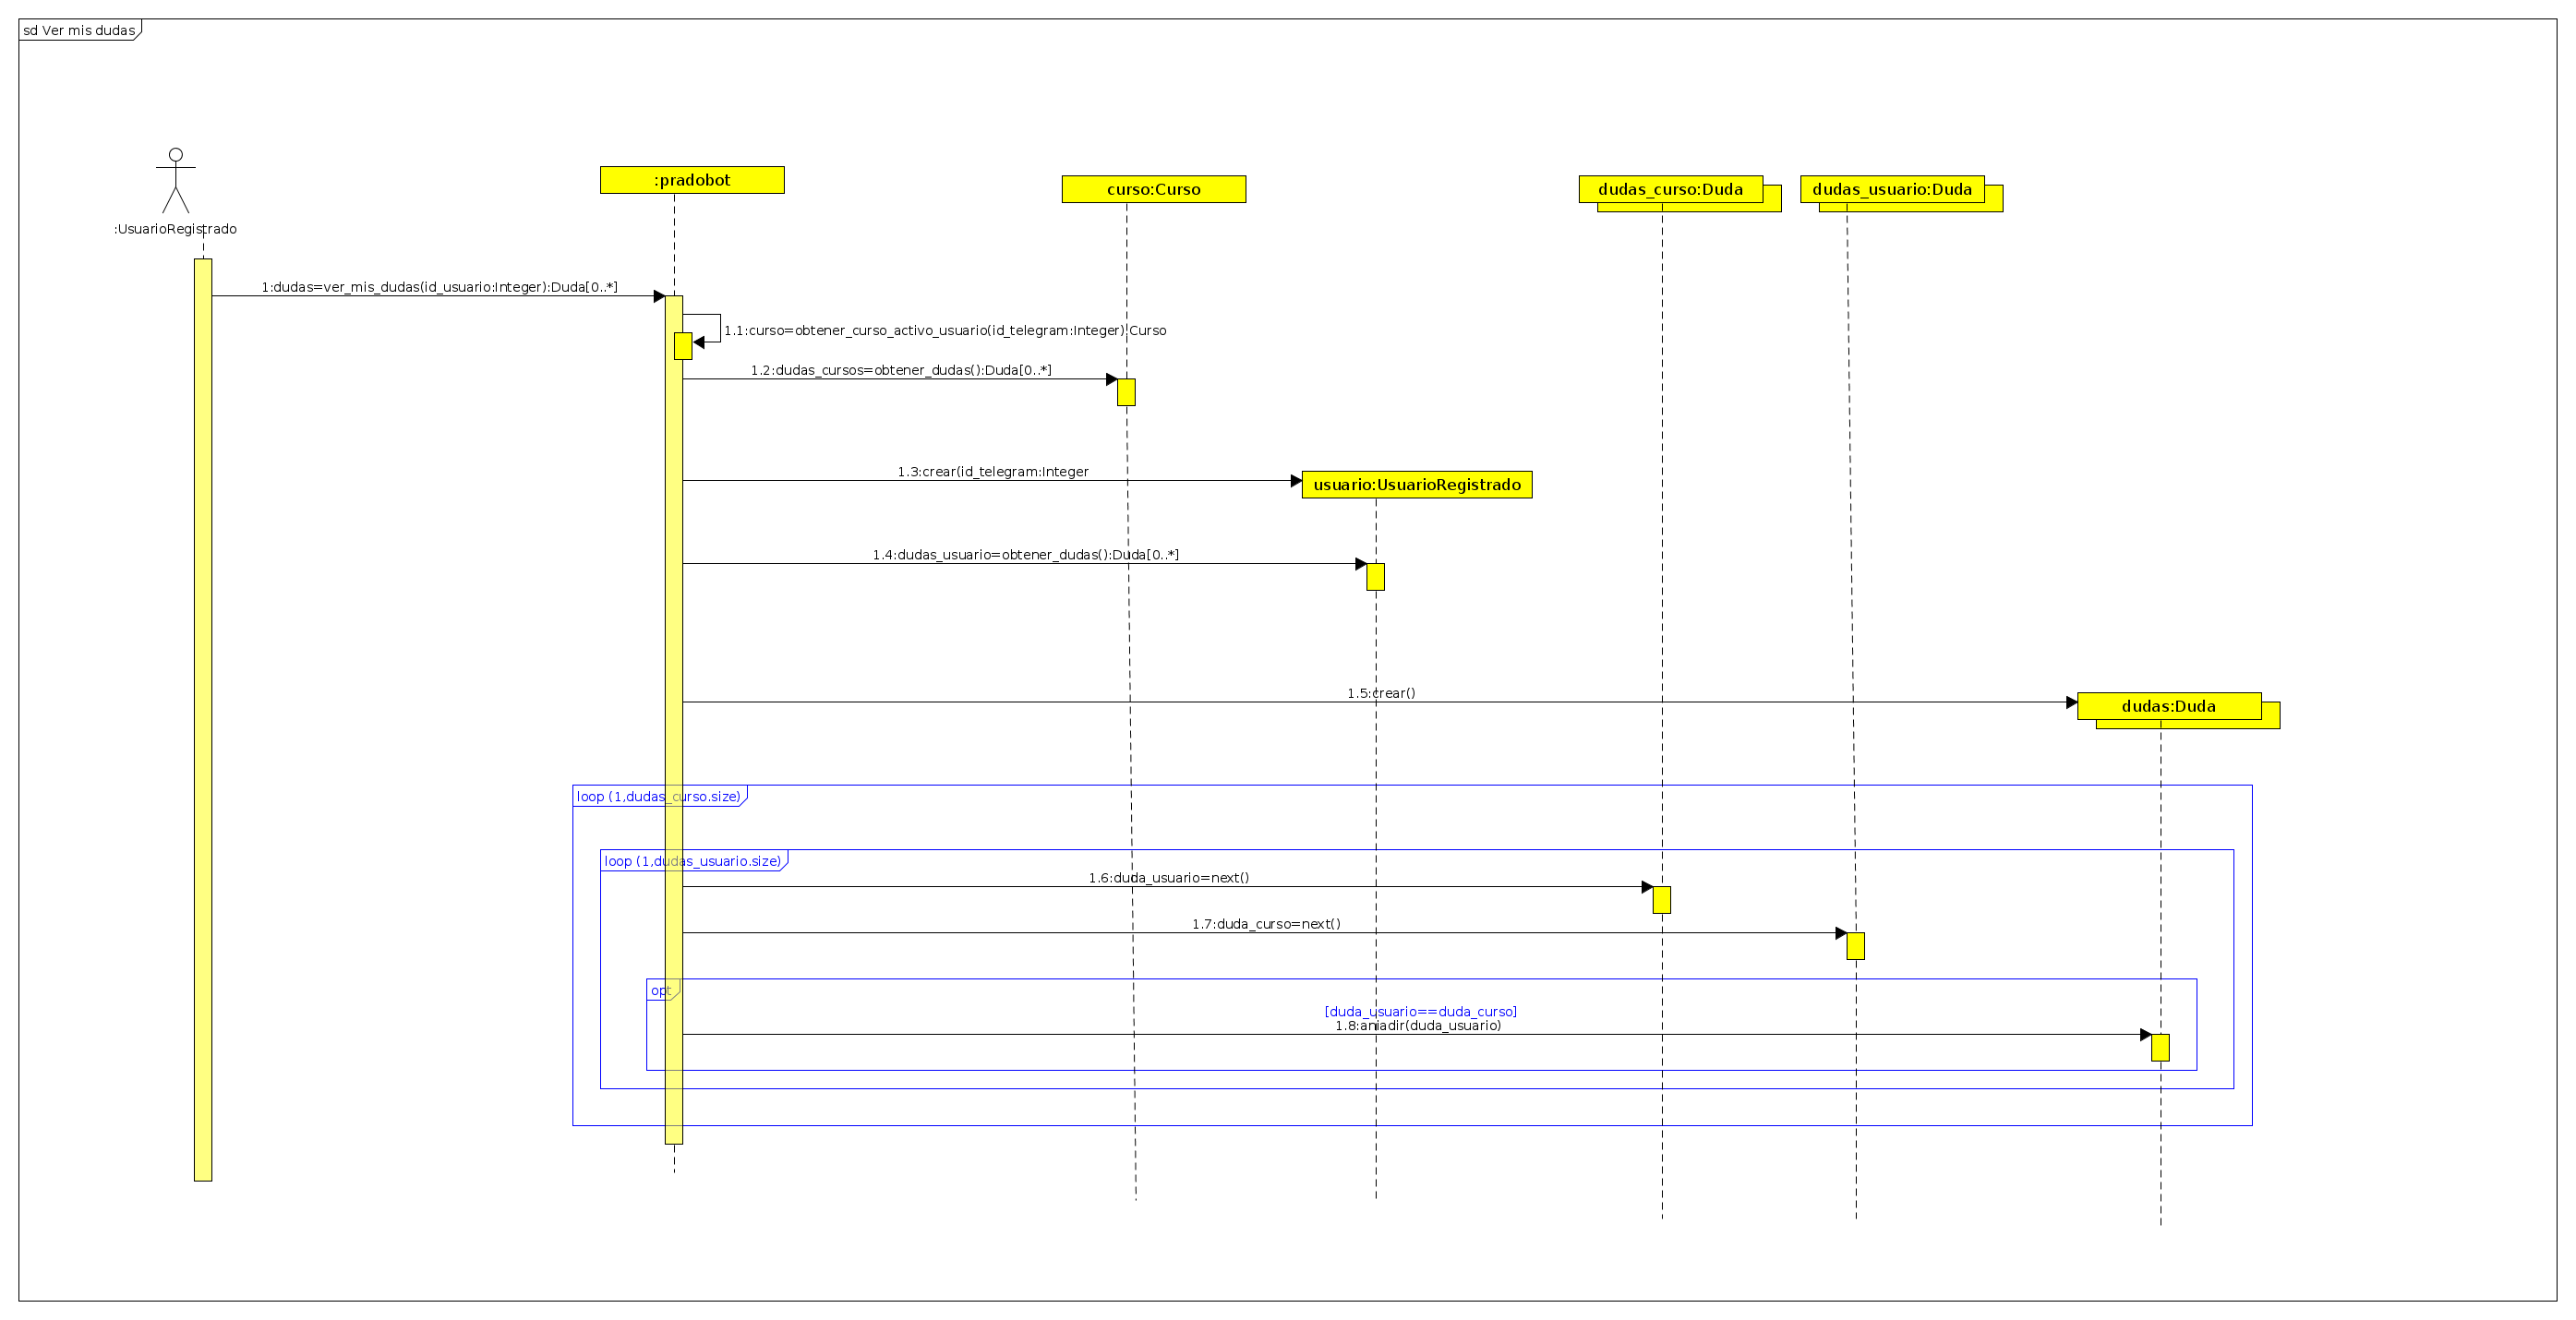
\includegraphics[scale=0.18]{imagenes/diagramas/secuencia/analisis/ver_mis_dudas.png}  %el parámetro scale permite agrandar o achicar la imagen. En el nombre de archivo puede especificar directorios

\caption{DS: Ver mis dudas (CU-5.3) }\label{figura84}

\end{figure}

\begin{figure}[H] %con el [H] le obligamos a situar aquí la figura
\centering
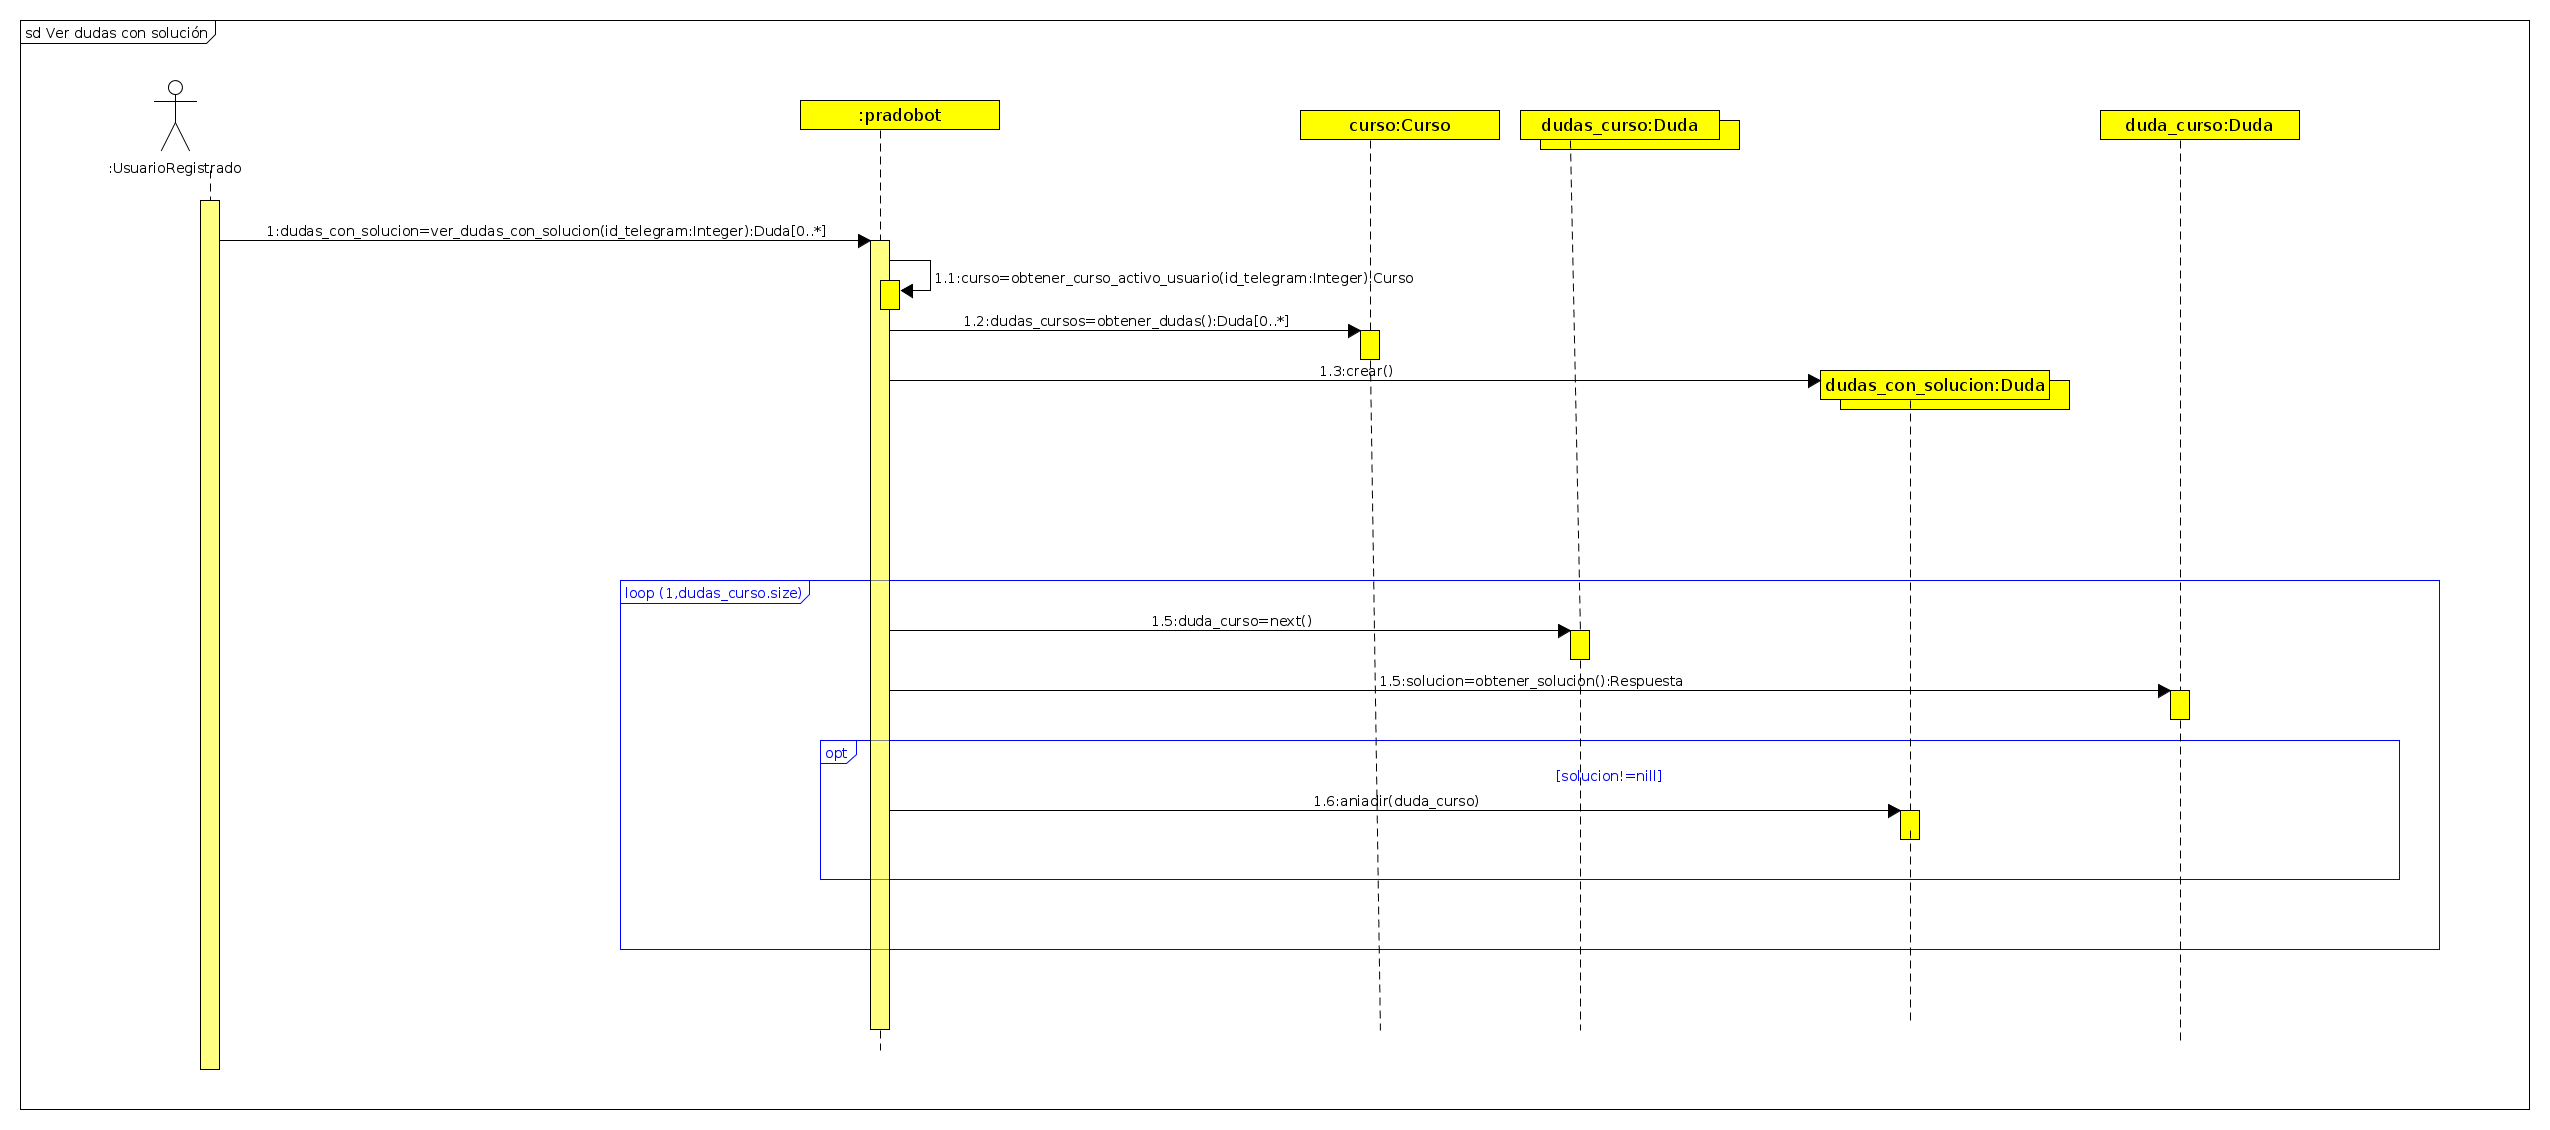
\includegraphics[scale=0.19]{imagenes/diagramas/secuencia/analisis/ver_dudas_resueltas.png}  %el parámetro scale permite agrandar o achicar la imagen. En el nombre de archivo puede especificar directorios

\caption{DS: Ver dudas con solución (CU-5.4) }\label{figura85}

\end{figure}


\begin{figure}[H] %con el [H] le obligamos a situar aquí la figura
\centering
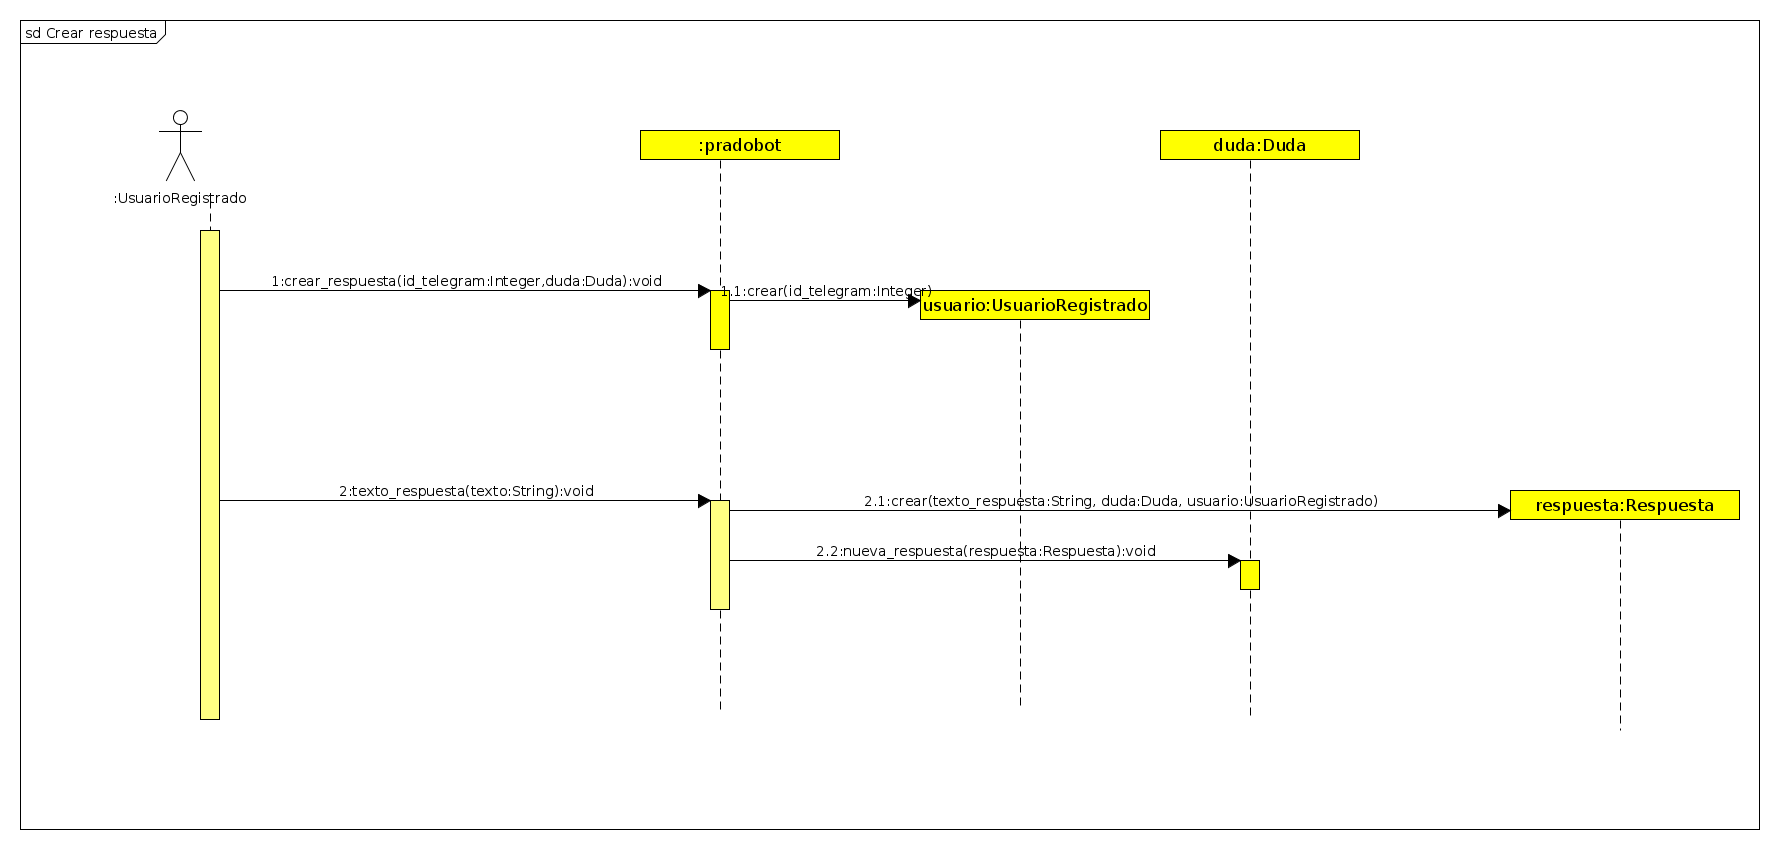
\includegraphics[scale=0.25]{imagenes/diagramas/secuencia/analisis/crear_respuesta.png}  %el parámetro scale permite agrandar o achicar la imagen. En el nombre de archivo puede especificar directorios

\caption{DS: Crear respuesta (CU-5.5) }\label{figura86}

\end{figure}

\begin{figure}[H] %con el [H] le obligamos a situar aquí la figura
\centering
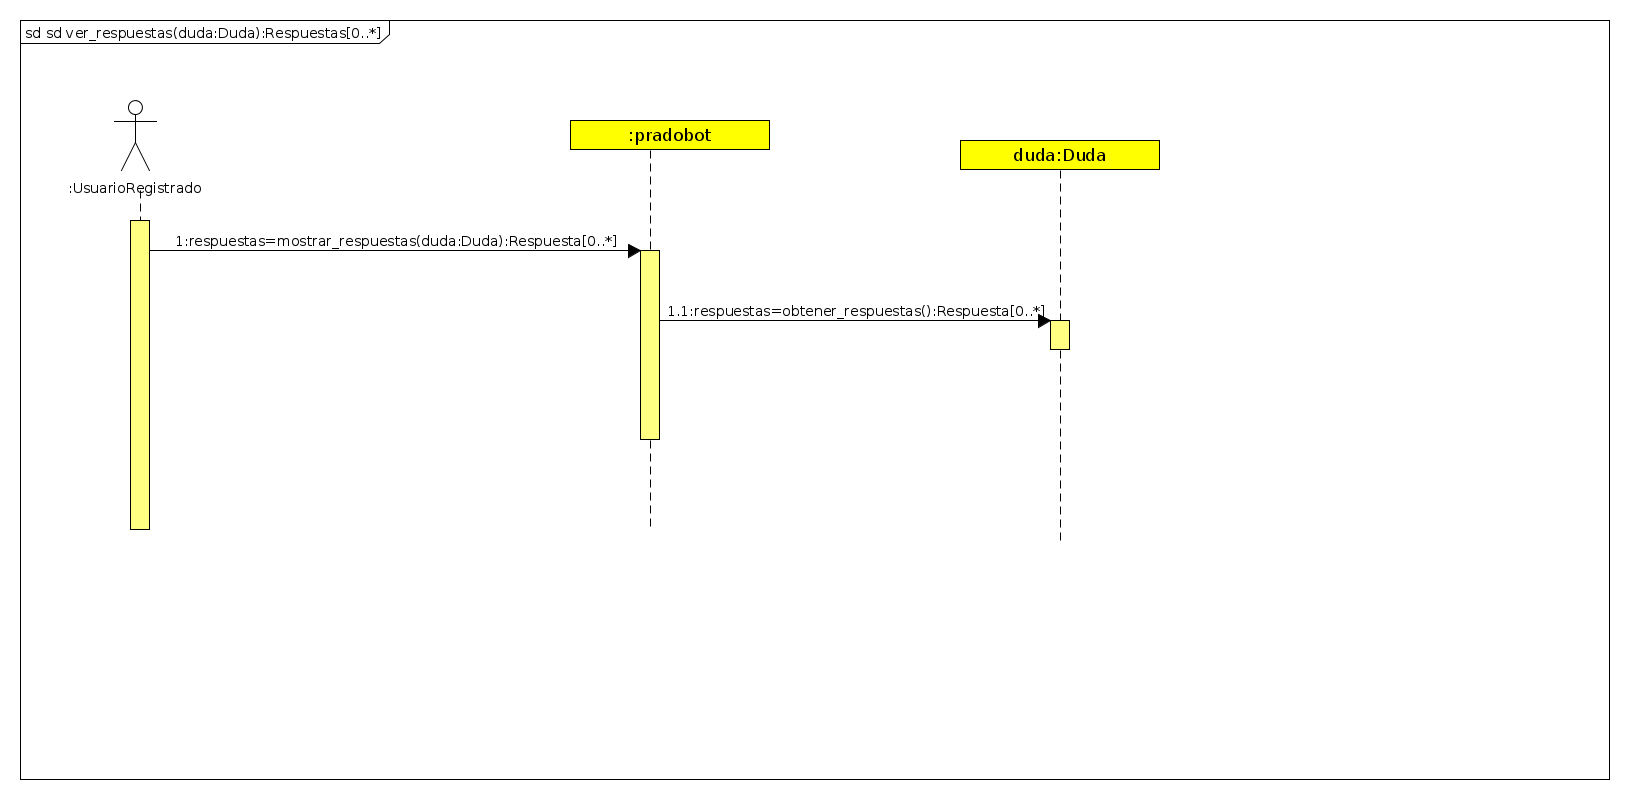
\includegraphics[scale=0.27]{imagenes/diagramas/secuencia/analisis/ver_respuestas_duda.png}  %el parámetro scale permite agrandar o achicar la imagen. En el nombre de archivo puede especificar directorios

\caption{DS: Ver respuestas (CU-5.6) }\label{figura87}

\end{figure}


\begin{figure}[H] %con el [H] le obligamos a situar aquí la figura
\centering
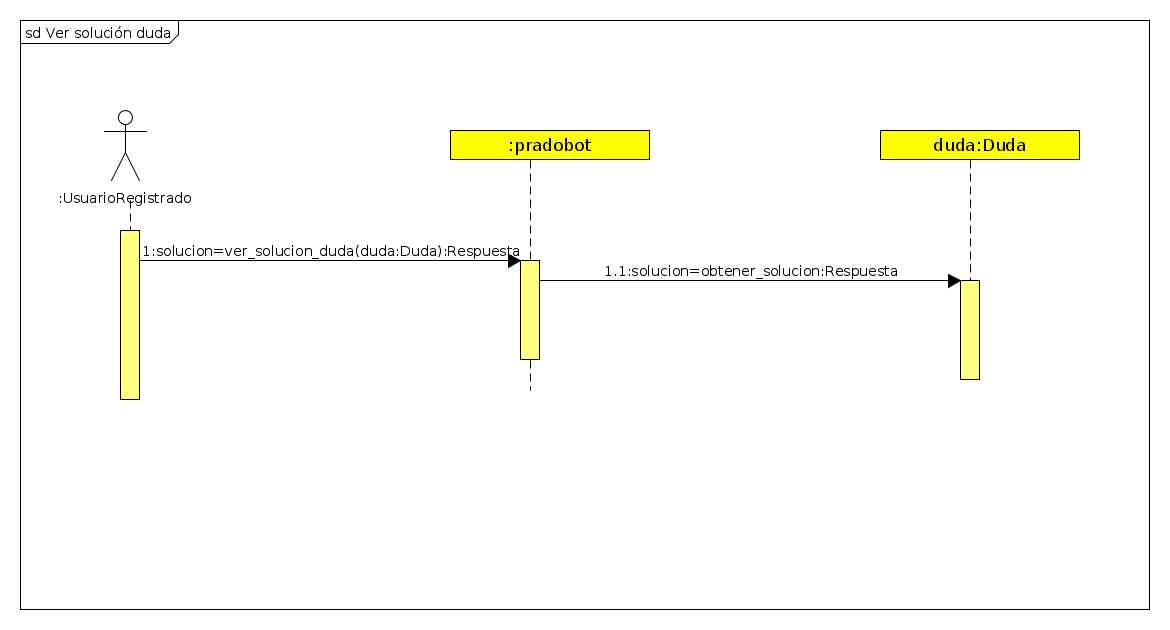
\includegraphics[scale=0.35]{imagenes/diagramas/secuencia/analisis/ver_solucion_duda.png}  %el parámetro scale permite agrandar o achicar la imagen. En el nombre de archivo puede especificar directorios

\caption{DS: Ver solución a duda (CU-5.7) }\label{figura88}

\end{figure}

\begin{figure}[H] %con el [H] le obligamos a situar aquí la figura
\centering
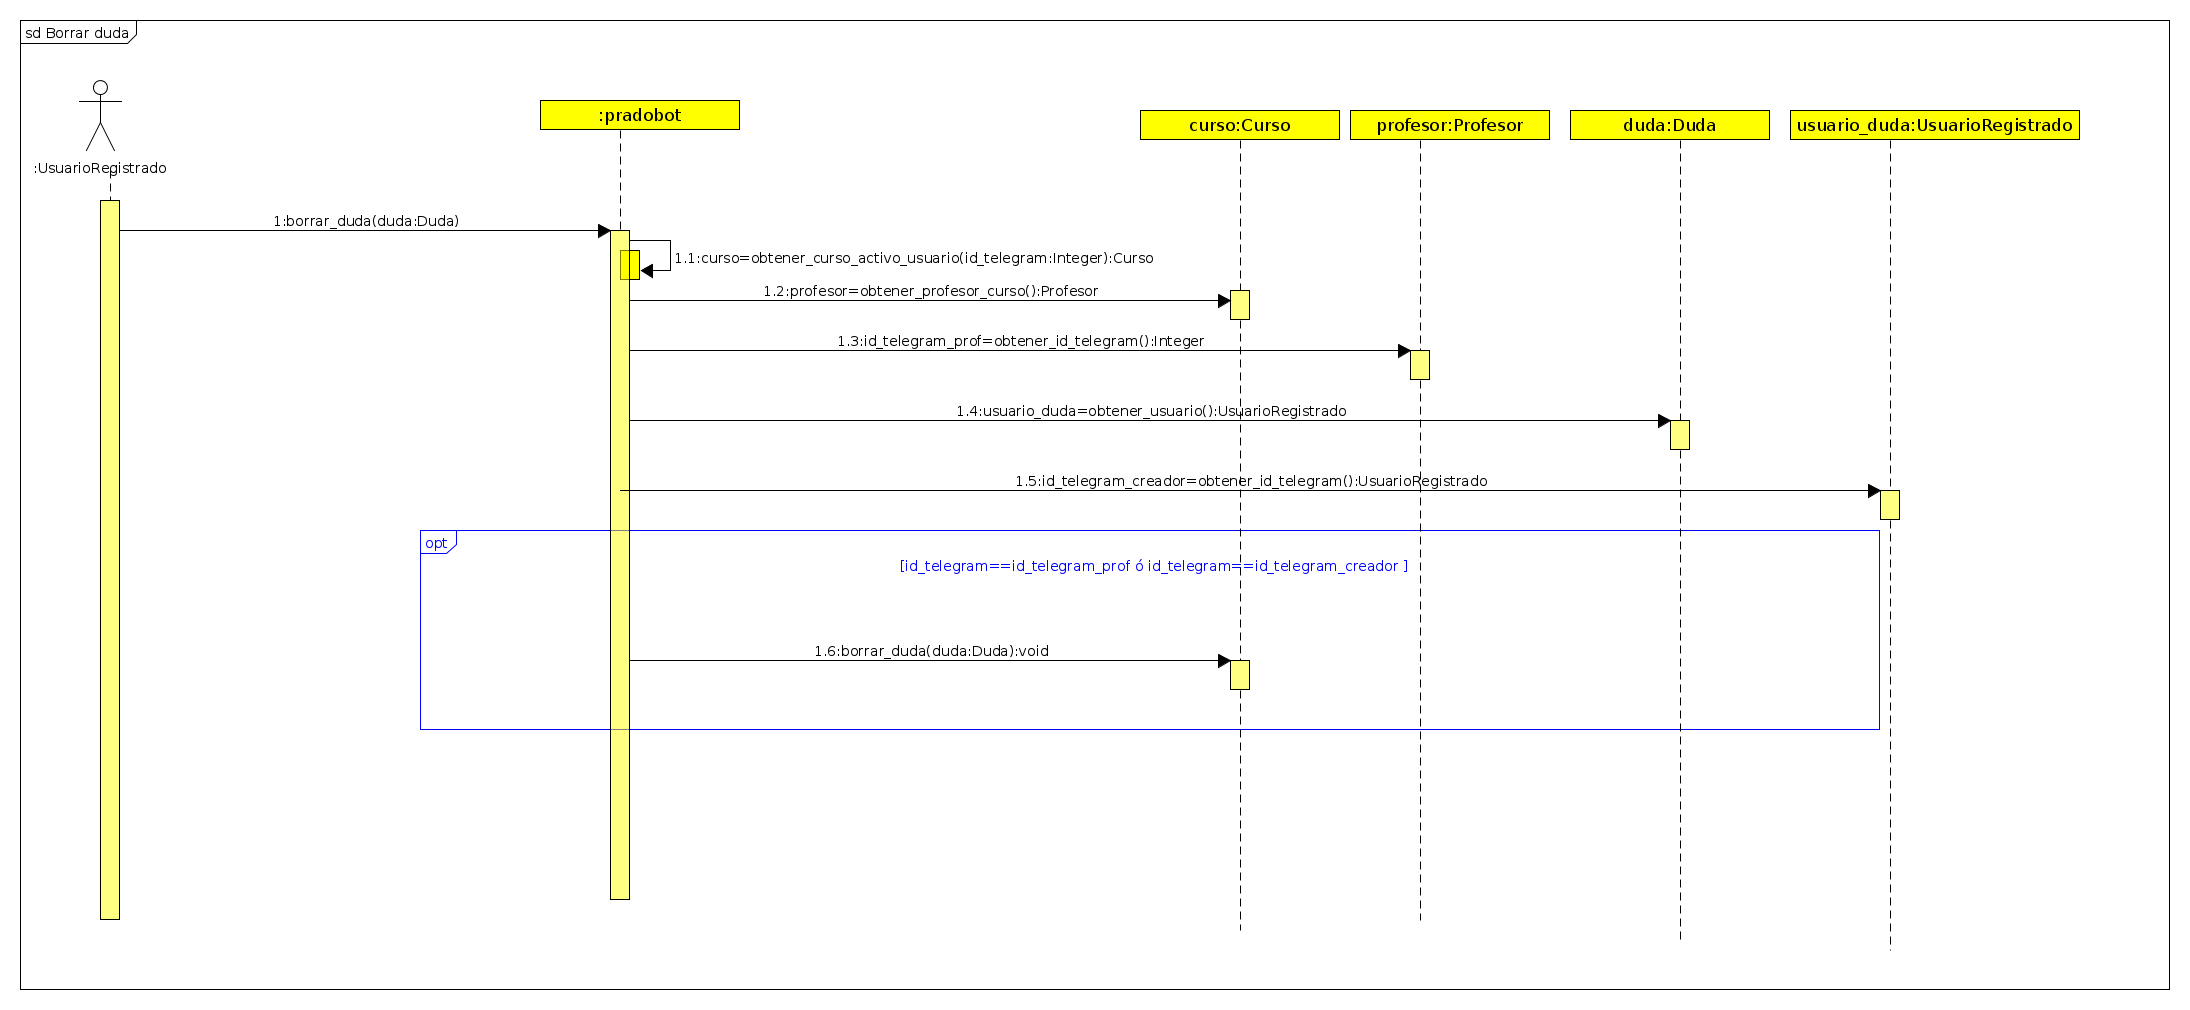
\includegraphics[scale=0.2]{imagenes/diagramas/secuencia/analisis/borrar_duda.png}  %el parámetro scale permite agrandar o achicar la imagen. En el nombre de archivo puede especificar directorios

\caption{DS: Borrar duda (CU-5.8, CU-5.10) }\label{figura89}

\end{figure}

\begin{figure}[H] %con el [H] le obligamos a situar aquí la figura
\centering
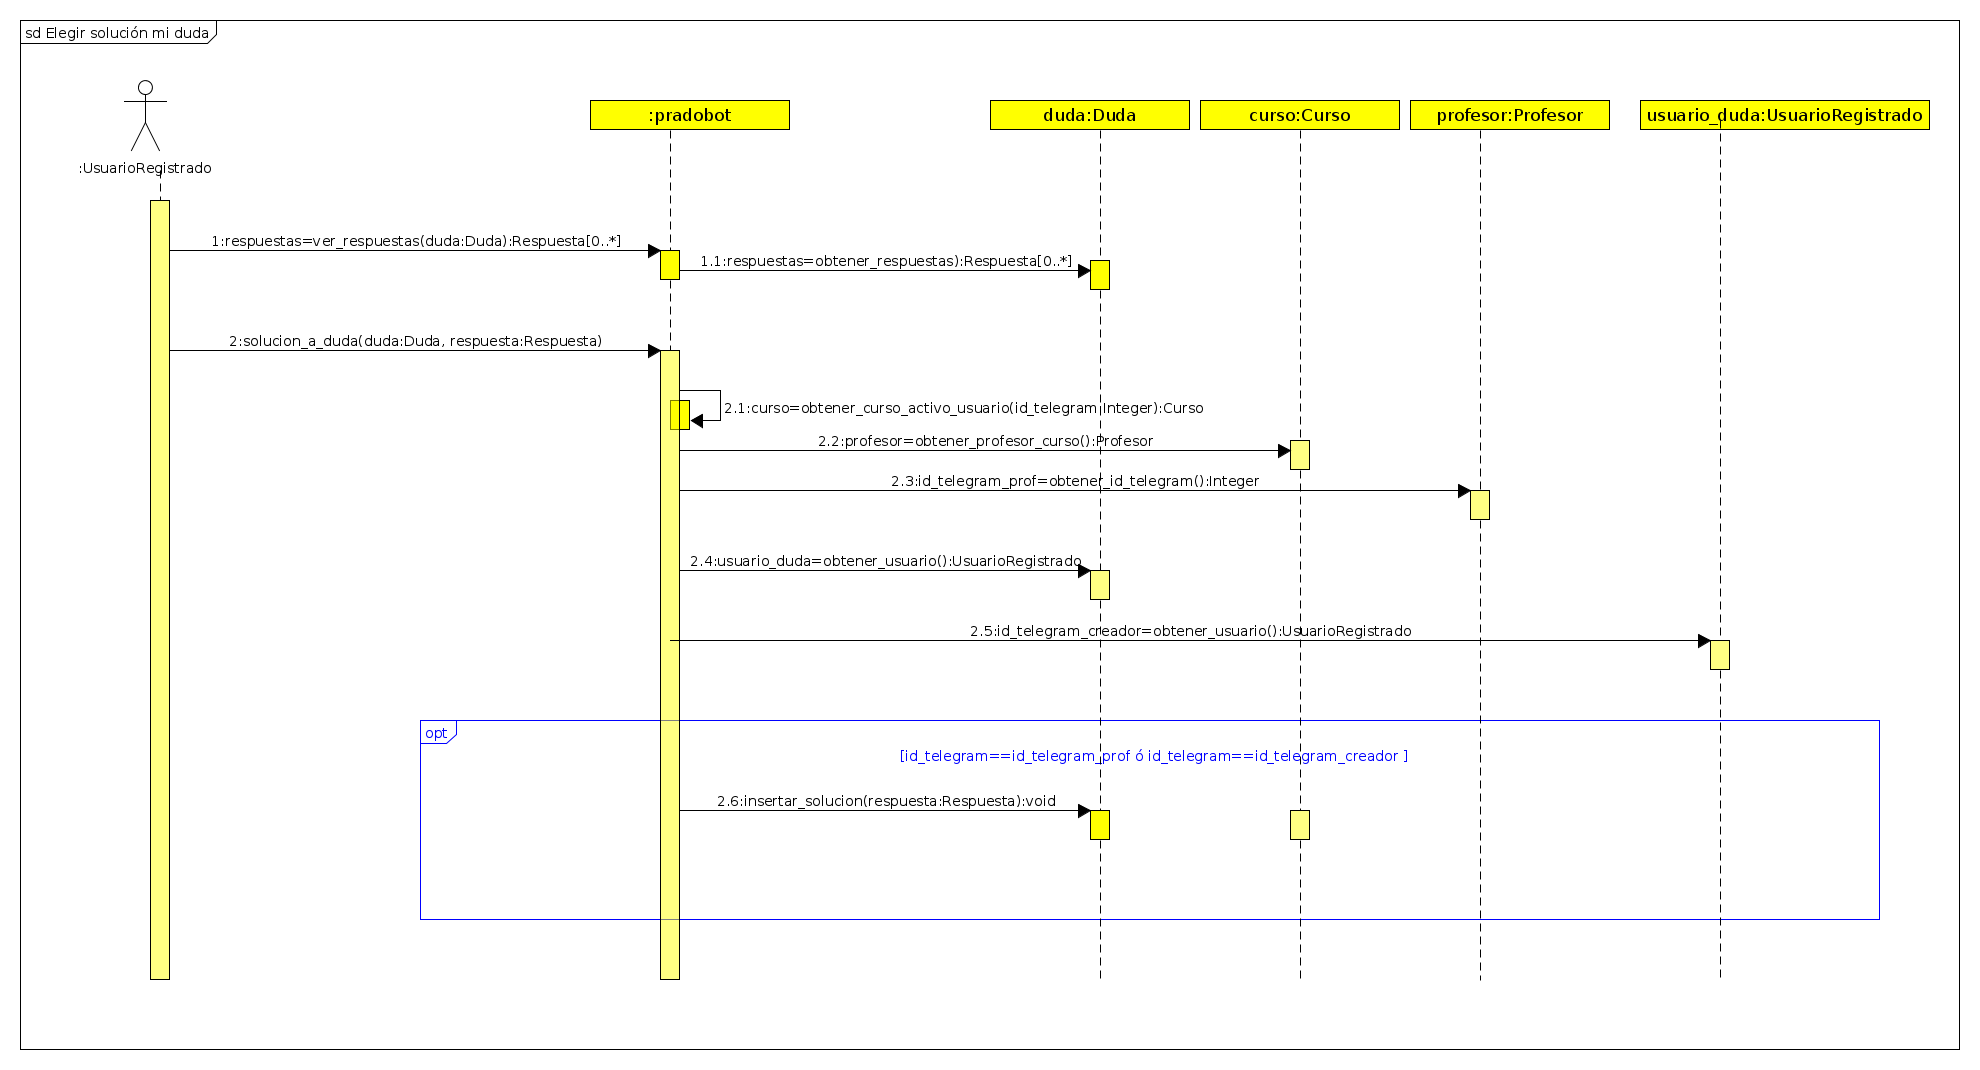
\includegraphics[scale=0.2]{imagenes/diagramas/secuencia/analisis/elegir_solucion_mi_duda.png}  %el parámetro scale permite agrandar o achicar la imagen. En el nombre de archivo puede especificar directorios

\caption{DS: Elegir solución duda (CU-5.9, CU-5.11) }\label{figura90}

\end{figure}


\begin{figure}[H] %con el [H] le obligamos a situar aquí la figura
\centering
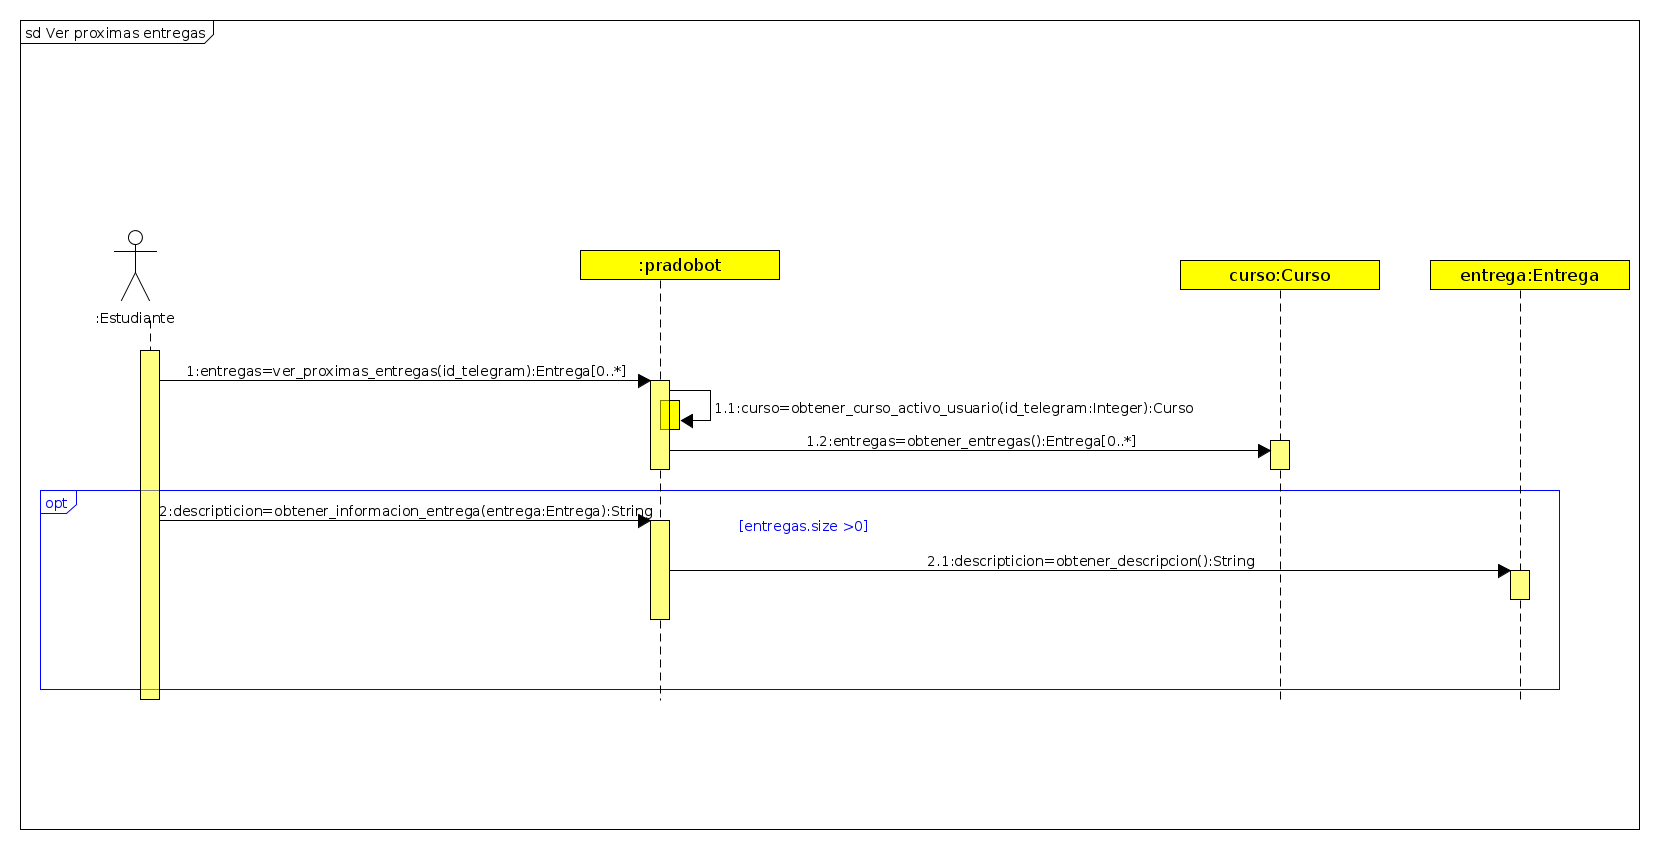
\includegraphics[scale=0.27]{imagenes/diagramas/secuencia/analisis/ver_proximas_entregas.png}  %el parámetro scale permite agrandar o achicar la imagen. En el nombre de archivo puede especificar directorios

\caption{DS: Ver proximas entregas (CU-6.1) }\label{figura91}

\end{figure}


\begin{figure}[H] %con el [H] le obligamos a situar aquí la figura
\centering
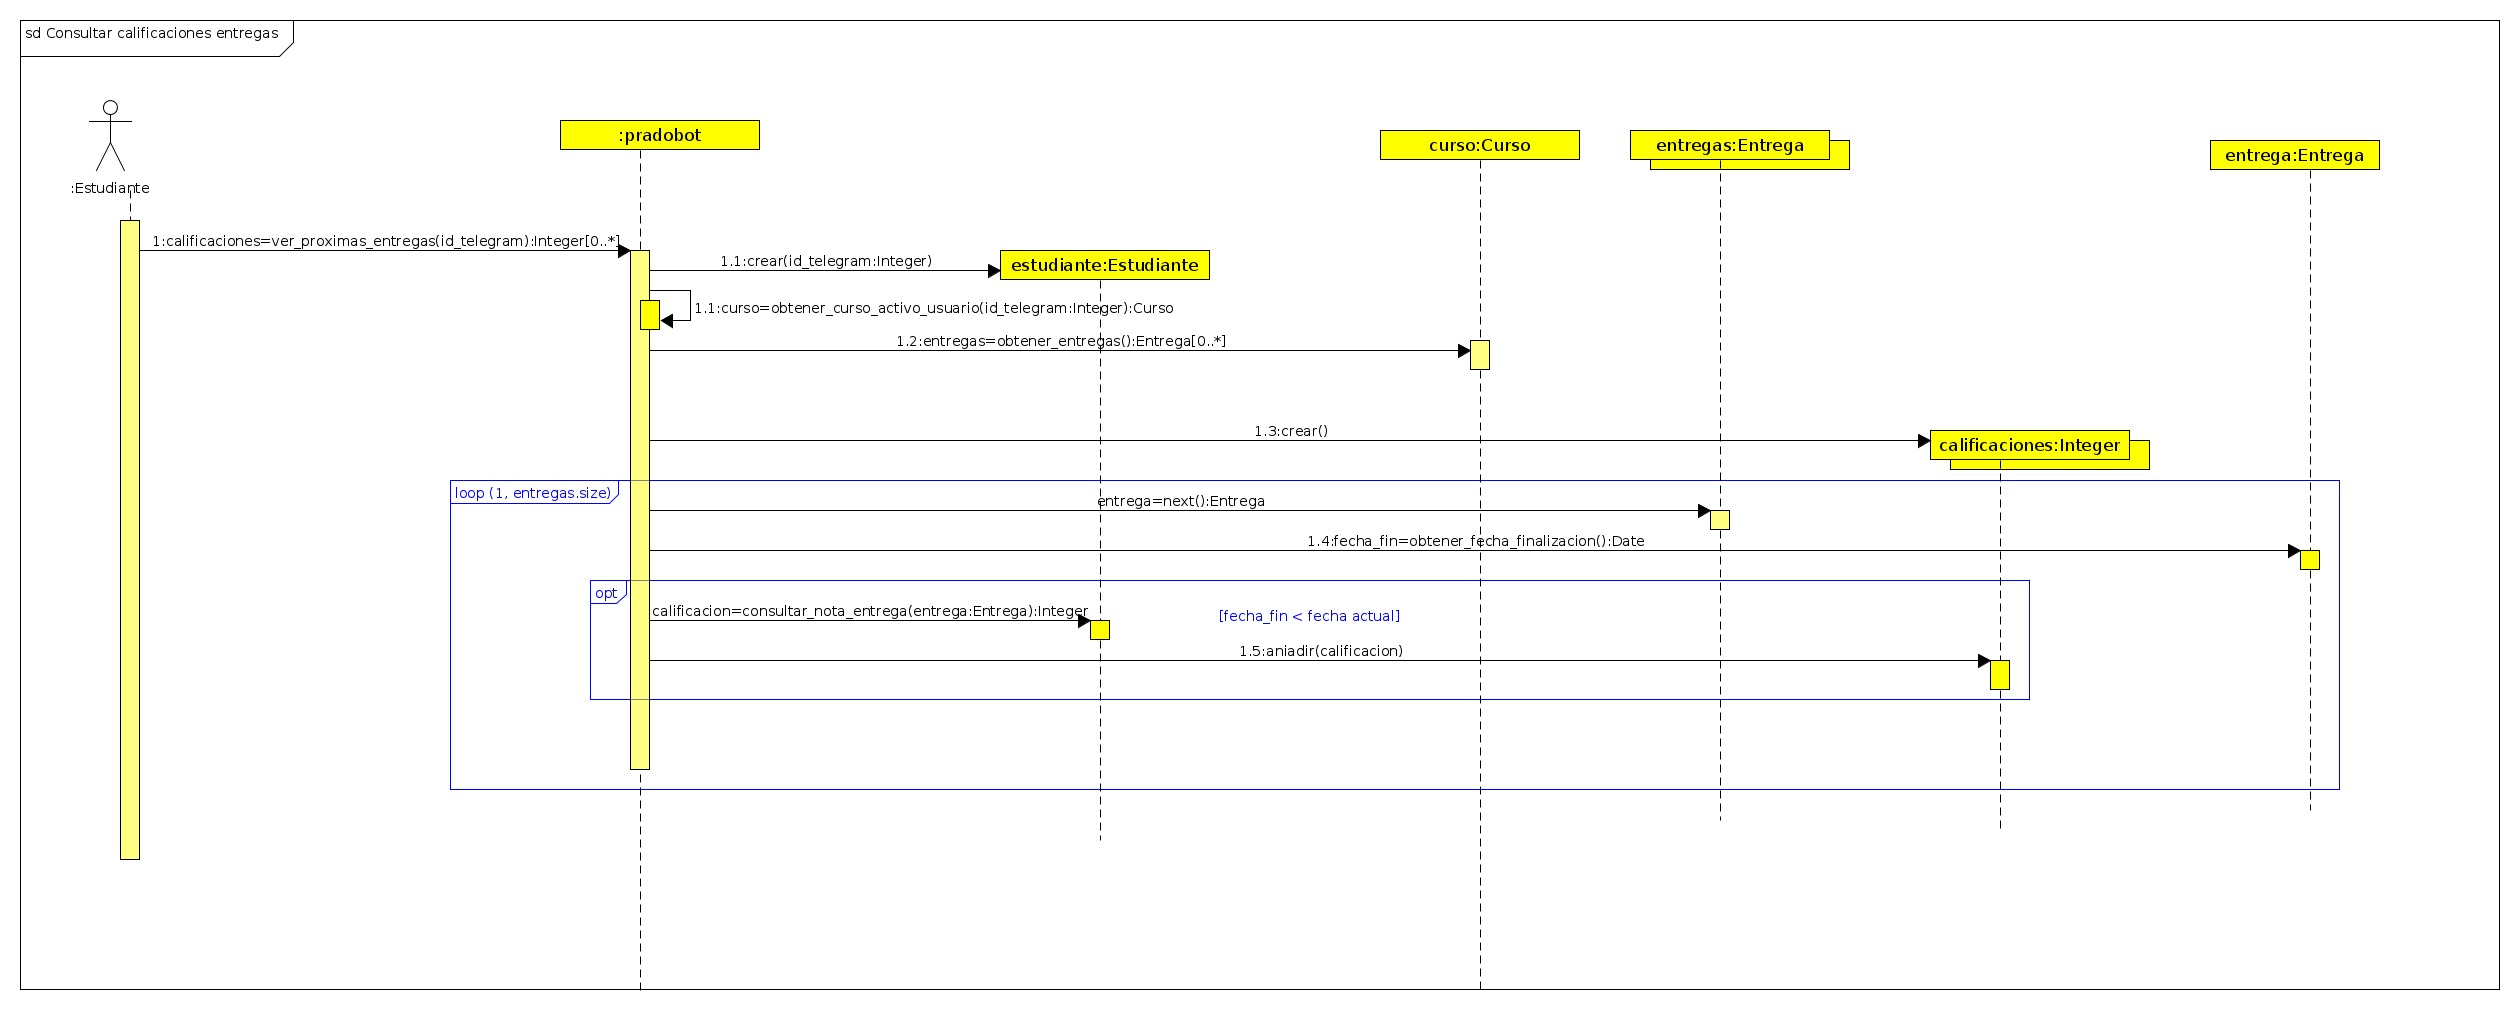
\includegraphics[scale=0.19]{imagenes/diagramas/secuencia/analisis/consultar_calificaciones_entregas.png}  %el parámetro scale permite agrandar o achicar la imagen. En el nombre de archivo puede especificar directorios

\caption{DS: Consultar calificaciones entregas (CU-6.2) }\label{figura92}

\end{figure}




\subsection{Contratos}
    %%%%%%%%%%%%%%%%%%%%%%%%%%%%%%%%%%%%%%%%%%%
   
   
               \begin{table}[!ht]
\begin{tabular}{|c|m{10cm}|}
\hline\rowcolor{Gray}
{\bf Nombre } & {tutorias=obtener\_tutorias()}\\
\hline
{\bf Responsabilidad } & {Obteniene las tutorías de un Profesor.}\\
\hline
\rowcolor{Gray}
{\bf Tipo } & {Profesor} \\
\hline
{\bf Notas } & { } \\
\hline
\rowcolor{Gray}
{\bf Excepciones }& {
\begin{itemize}
\item Que no tenga tutorías el objeto profesor.
\end{itemize}
} \\
\hline
{\bf Salida }& 

	  { 	
	  Para cada objeto tipo Tutoria contenido en tutorias se proporciona:
	  \begin{itemize}
	  \item \enquote{El profesor que la ha creado}
	  \item \enquote{Fecha tutoría}
	  \end{itemize}
	  } 


 \\
\hline
\rowcolor{Gray}
{\bf Precondiciones }& {}\\
\hline
{\bf Poscondiciones }& {
}  \\
\hline
\end{tabular}

\end{table}

 
               \begin{table}[!ht]
\begin{tabular}{|c|m{10cm}|}
\hline\rowcolor{Gray}
{\bf Nombre } & {peticiones=obtener\_peticiones()}\\
\hline
{\bf Responsabilidad } & {Obtiene las peticiones que ha recibido una Tutoria}\\
\hline
\rowcolor{Gray}
{\bf Tipo } & {Tutoria} \\
\hline
{\bf Notas } & { } \\
\hline
\rowcolor{Gray}
{\bf Excepciones }& {
\begin{itemize}
\item Que no haya tenido ninguna petición la tutoría.
\end{itemize}
} \\
\hline
{\bf Salida }& 

	  { 	
	  Para cada objeto Peticion contenido en peticiones se proporciona:
	  \begin{itemize}
	  \item La tutoría a la que se ha realizado la petición
	  \item El estudiante que ha realizado la petición
	  \end{itemize}
	  } 


 \\
\hline
\rowcolor{Gray}
{\bf Precondiciones }& {}\\
\hline
{\bf Poscondiciones }& {
}  \\
\hline
\end{tabular}

\end{table}    
    
    
    
    
    
    
                  \begin{table}[!ht]
\begin{tabular}{|c|m{10cm}|}
\hline\rowcolor{Gray}
{\bf Nombre } & {denegar()}\\
\hline
{\bf Responsabilidad } & {Cambia el estado de  una petición a rechazada}\\
\hline
\rowcolor{Gray}
{\bf Tipo } & {Peticion} \\
\hline
{\bf Notas } & { } \\
\hline
\rowcolor{Gray}
{\bf Excepciones }& {

} \\
\hline
{\bf Salida }& 
	  { 	

	  } 
 \\
\hline
\rowcolor{Gray}
{\bf Precondiciones }& {}\\
\hline
{\bf Poscondiciones }& { Fue modificado el objeto de la clase Peticion cambiándose el valor del atributo estado a \enquote*{rechazada}.
}  \\
\hline
\end{tabular}

\end{table} 
    
    
                      \begin{table}[!ht]
\begin{tabular}{|c|m{10cm}|}
\hline\rowcolor{Gray}
{\bf Nombre } & {aceptar()}\\
\hline
{\bf Responsabilidad } & {Cambia el estado de una Peticion a aceptada}\\
\hline
\rowcolor{Gray}
{\bf Tipo } & {Peticion} \\
\hline
{\bf Notas } & { } \\
\hline
\rowcolor{Gray}
{\bf Excepciones }& {

} \\
\hline
{\bf Salida }& 
	  { 	
	  } 
 \\
\hline
\rowcolor{Gray}
{\bf Precondiciones }& {}\\
\hline
{\bf Poscondiciones }& { El valor del atributo estado del objeto de la clase Peticion fue modificado a \enquote*{aceptada}.
}  \\
\hline
\end{tabular}

\end{table} 


    
                      \begin{table}[!ht]
\begin{tabular}{|c|m{10cm}|}
\hline\rowcolor{Gray}
{\bf Nombre } & {profesor=obtener\_profesor\_curso()}\\
\hline
{\bf Responsabilidad } & {Obteniene a el Profesor responsable de un Curso}\\
\hline
\rowcolor{Gray}
{\bf Tipo } & {Curso} \\
\hline
{\bf Notas } & { } \\
\hline
\rowcolor{Gray}
{\bf Excepciones }& {

} \\
\hline
{\bf Salida }& 
	  { 	
	  Para el objeto profesor de la clase Profesor contenido en profesor se proporciona
	  \begin{itemize}
	  \item id\_telegram
	  \end{itemize}
	  } 
 \\
\hline
\rowcolor{Gray}
{\bf Precondiciones }& {}\\
\hline
{\bf Poscondiciones }& {}.
  \\
\hline
\end{tabular}

\end{table}
 
 
                       \begin{table}[!ht]
\begin{tabular}{|c|m{10cm}|}
\hline\rowcolor{Gray}
{\bf Nombre } & {aceptada=solicitar\_tutoria(peticion)}\\
\hline
{\bf Responsabilidad } & {Realiza una Peticion a una tutoría de un Profesor.}\\
\hline
\rowcolor{Gray}
{\bf Tipo } & {Profesor} \\
\hline
{\bf Notas } & { } \\
\hline
\rowcolor{Gray}
{\bf Excepciones }& {
	  \begin{itemize}
	  \item El estudiante que realiza la petición ya haya realizado otra a la misma tutoría.
	  \item El objeto estudiante de la clase Estudiante contenido en petición no exista.
	  \end{itemize}
} \\
\hline
{\bf Salida }& 
	  { 	
	  Para el objeto aceptada de  la clase Boolean se proporciona el valor true o false.
	  } 
 \\
\hline
\rowcolor{Gray}
{\bf Precondiciones }& {}\\
\hline
{\bf Poscondiciones }& {
\begin{itemize}
\item Fue creado un enlace entre el objeto peticion de la clase Peticion y el objeto de la clase Tutoria
\end{itemize}}
  \\
\hline
\end{tabular}

\end{table}


                       \begin{table}[!ht]
\begin{tabular}{|c|m{10cm}|}
\hline\rowcolor{Gray}
{\bf Nombre } & {id\_telegram=obtener\_telegram()}\\
\hline
{\bf Responsabilidad } & {Obteniene el identificador de Telegram un Profesor}\\
\hline
\rowcolor{Gray}
{\bf Tipo } & {Profesor} \\
\hline
{\bf Notas } & { } \\
\hline
\rowcolor{Gray}
{\bf Excepciones }& {
} \\
\hline
{\bf Salida }& 
	  { 	
	  Devuelve identificador numérico en el objeto de la clase Integer contenido en id\_telegram.
	  } 
 \\
\hline
\rowcolor{Gray}
{\bf Precondiciones }& {}\\
\hline
{\bf Poscondiciones }& {}.
  \\
\hline
\end{tabular}

\end{table}



                       \begin{table}[!ht]
\begin{tabular}{|c|m{10cm}|}
\hline\rowcolor{Gray}
{\bf Nombre } & {usuario\_duda=obtener\_usuario()}\\
\hline
{\bf Responsabilidad } & {Obteniene al UsuarioRegistrado creador de una Duda}\\
\hline
\rowcolor{Gray}
{\bf Tipo } & {Profesor} \\
\hline
{\bf Notas } & { } \\
\hline
\rowcolor{Gray}
{\bf Excepciones }& {
} \\
\hline
{\bf Salida }& 
	  { 	
	  Para el objeto UsuarioRegistrado contenido en usuario\_duda se proporciona:
	  \begin{itemize}
	  \item id\_telegram
	  \end{itemize}
	  } 
 \\
\hline
\rowcolor{Gray}
{\bf Precondiciones }& {}\\
\hline
{\bf Poscondiciones }& {}.
  \\
\hline
\end{tabular}

\end{table}



                       \begin{table}[!ht]
\begin{tabular}{|c|m{10cm}|}
\hline\rowcolor{Gray}
{\bf Nombre } & {id\_telegram=obtener\_telegram()}\\
\hline
{\bf Responsabilidad } & {Obtiene el identificador numérico de un UsuarioRegistrado}\\
\hline
\rowcolor{Gray}
{\bf Tipo } & {UsuarioRegistrado} \\
\hline
{\bf Notas } & { } \\
\hline
\rowcolor{Gray}
{\bf Excepciones }& {
} \\
\hline
{\bf Salida }& 
	  { 	
	  Devuelve identificador numérico para el objeto id\_telegram de la clase Integer.
	  } 
 \\
\hline
\rowcolor{Gray}
{\bf Precondiciones }& {}\\
\hline
{\bf Poscondiciones }& {}
  \\
\hline
\end{tabular}

\end{table}



                       \begin{table}[!ht]
\begin{tabular}{|c|m{10cm}|}
\hline\rowcolor{Gray}
{\bf Nombre } & {borrar\_duda(duda)}\\
\hline
{\bf Responsabilidad } & {Borra una Duda de un Curso}\\
\hline
\rowcolor{Gray}
{\bf Tipo } & {Curso} \\
\hline
{\bf Notas } & { } \\
\hline
\rowcolor{Gray}
{\bf Excepciones }& {
\begin{itemize}
\item Que no exista el objeto duda de la clase Duda.
\end{itemize}
} \\
\hline
{\bf Salida }& 
	  { 	
	  } 
 \\
\hline
\rowcolor{Gray}
{\bf Precondiciones }& {
}\\
\hline
{\bf Poscondiciones }& {

\begin{itemize}
\item Fue borrado el enlace entre el objeto duda y el el objeto de la clase Curso .
\item Para cada objeto r de la clase Respuesta relacionado con el objeto duda de la clase Duda:
\begin{itemize}
\item Fue borrado el enlace entre r y duda.
\item Fue borrado el objeto r.
\end{itemize}
\item Fue borrado el enlace entre duda y el objeto de clase UsuarioRegistrado relacionado con duda.
\item Fue borrado el objeto duda.
\end{itemize}

}.
 \\
\hline
\end{tabular}

\end{table}

                       \begin{table}[!ht]
\begin{tabular}{|c|m{10cm}|}
\hline\rowcolor{Gray}
{\bf Nombre } & {borrar\_tutoria(tutoria)}\\
\hline
{\bf Responsabilidad } & {Elimina una Tutoria de un Profesor}\\
\hline
\rowcolor{Gray}
{\bf Tipo } & {Profesor} \\
\hline
{\bf Notas } & { } \\
\hline
\rowcolor{Gray}
{\bf Excepciones }& {
\begin{itemize}
\item Que no exista el objeto tutoria de la clase Tutoria.
\end{itemize}
} \\
\hline
{\bf Salida }& 
	  { 	
	  } 
 \\
\hline
\rowcolor{Gray}
{\bf Precondiciones }& {
}\\
\hline
{\bf Poscondiciones }& {

\begin{itemize}
\item Fue borrado el enlace entre el objeto tutoria y el el objeto de la clase Profesor .
\item Para cada objeto p de la clase Petición relacionado con el objeto tutoria de la clase Tutoria:
\begin{itemize}
\item Fue borrado el enlace entre p y tutoria.
\item Fue borrado el enlace entre p y el objeto de la clase Estudiante con el que está relacionado.
\item Fue borrado el objeto p.
\end{itemize}
\item Fue borrado el objeto tutoria
\end{itemize}

}.
  \\
\hline
\end{tabular}

\end{table}


                       \begin{table}[!ht]
\begin{tabular}{|c|m{10cm}|}
\hline\rowcolor{Gray}
{\bf Nombre } & {entregas=obtener\_entregas()}\\
\hline
{\bf Responsabilidad } & {Obtener las entregas de un Curso}\\
\hline
\rowcolor{Gray}
{\bf Tipo } & {Profesor} \\
\hline
{\bf Notas } & { } \\
\hline
\rowcolor{Gray}
{\bf Excepciones }& {
\begin{itemize}
\item No tenga ninguna entrega el objeto de la clase Curso.
\end{itemize}
} \\
\hline
{\bf Salida }& 
	  { 	
	  Para cada objeto Entrega contenido en entregas se proporciona:
	  \begin{itemize}
	  \item fecha\_fin
	  \item identificador
	  \item nombre
	  \end{itemize}	  } 
 \\
\hline
\rowcolor{Gray}
{\bf Precondiciones }& {
}\\
\hline
{\bf Poscondiciones }& {
}
  \\
\hline
\end{tabular}

\end{table}




                       \begin{table}[!ht]
\begin{tabular}{|c|m{10cm}|}
\hline\rowcolor{Gray}
{\bf Nombre } & {fecha\_fin=obtener\_fecha\_finalizacion()}\\
\hline
{\bf Responsabilidad } & {Obteniene la fecha finalización de una Entrega}\\
\hline
\rowcolor{Gray}
{\bf Tipo } & {Entrega} \\
\hline
{\bf Notas } & { } \\
\hline
\rowcolor{Gray}
{\bf Excepciones }& {
} \\
\hline
{\bf Salida }& 
	  { 	
	  Se devuelve el valor del atributo fecha\_fin del objeto de la clase Entrega en el objeto tipo Date contenido en fecha\_fin } 
 \\
\hline
\rowcolor{Gray}
{\bf Precondiciones }& {
}\\
\hline
{\bf Poscondiciones }& {
}
  \\
\hline
\end{tabular}

\end{table}




                       \begin{table}[!ht]
\begin{tabular}{|c|m{10cm}|}
\hline\rowcolor{Gray}
{\bf Nombre } & {aniadir\_duda(duda)}\\
\hline
{\bf Responsabilidad } & {Añade una nueva Duda al Curso}\\
\hline
\rowcolor{Gray}
{\bf Tipo } & {Curso} \\
\hline
{\bf Notas } & { } \\
\hline
\rowcolor{Gray}
{\bf Excepciones }& {
} \\
\hline
{\bf Salida }& 
	  { 	
 } 
 \\
\hline
\rowcolor{Gray}
{\bf Precondiciones }& {
}\\
\hline
{\bf Poscondiciones }& {
\begin{itemize}
\item Fue creado un enlace entre el objeto duda de la clase Duda y el objeto de la clase Curso.
\end{itemize}
}
  \\
\hline
\end{tabular}

\end{table}








                       \begin{table}[!ht]
\begin{tabular}{|c|m{10cm}|}
\hline\rowcolor{Gray}
{\bf Nombre } & {nueva\_respuesta(respuesta)}\\
\hline
{\bf Responsabilidad } & {Añade una nueva Respuesta a una Duda}\\
\hline
\rowcolor{Gray}
{\bf Tipo } & {Duda} \\
\hline
{\bf Notas } & { } \\
\hline
\rowcolor{Gray}
{\bf Excepciones }& {
} \\
\hline
{\bf Salida }& 
	  { 	
} 
 \\
\hline
\rowcolor{Gray}
{\bf Precondiciones }& {
}\\
\hline
{\bf Poscondiciones }& { Fue creado un enlace entre el objeto respuesta de la clase Respuesta y el objeto de la clase Duda.
}
  \\
\hline
\end{tabular}

\end{table}






                       \begin{table}[!ht]
\begin{tabular}{|c|m{10cm}|}
\hline\rowcolor{Gray}
{\bf Nombre } & {cursos=obtener\_cursos()}\\
\hline
{\bf Responsabilidad } & {Obtiene los cursos en los que está dado de alta un UsuarioRegistrado}\\
\hline
\rowcolor{Gray}
{\bf Tipo } & {UsuarioRegistrado} \\
\hline
{\bf Notas } & { } \\
\hline
\rowcolor{Gray}
{\bf Excepciones }& {
} \\
\hline
{\bf Salida }& 
	  {
Para cada objeto Curso contenido en cursos se proporciona:	  
	   	\begin{itemize}
	  \item id\_curso
	  \item nombre\_curso
	    \end{itemize}
} 
 \\
\hline
\rowcolor{Gray}
{\bf Precondiciones }& {
}\\
\hline
{\bf Poscondiciones }& { }
  \\
\hline
\end{tabular}

\end{table}





                       \begin{table}[!ht]
\begin{tabular}{|c|m{10cm}|}
\hline\rowcolor{Gray}
{\bf Nombre } & {respuestas=obtener\_respuestas()}\\
\hline
{\bf Responsabilidad } & {Obtiene las respuestas que tiene una Duda}\\
\hline
\rowcolor{Gray}
{\bf Tipo } & {Duda} \\
\hline
{\bf Notas } & { } \\
\hline
\rowcolor{Gray}
{\bf Excepciones }& {
\begin{itemize}
\item Que no haya tenido ninguna respuesta la duda.
\end{itemize}
} \\
\hline
{\bf Salida }& 
	  {
Para cada objeto Respuesta contenido en respuestas se proporciona:	  
	   	\begin{itemize}
	  \item contenido
	  \item usuario
	  \item duda
	    \end{itemize}
} 
 \\
\hline
\rowcolor{Gray}
{\bf Precondiciones }& {
}\\
\hline
{\bf Poscondiciones }& { }
  \\
\hline
\end{tabular}

\end{table}





\clearpage

                       \begin{table}[!ht]
\begin{tabular}{|c|m{10cm}|}
\hline\rowcolor{Gray}
{\bf Nombre } & {insertar\_solucion(respuesta:Respuesta)}\\
\hline
{\bf Responsabilidad } & {Asigna una Respuesta como solución a una Duda}\\
\hline
\rowcolor{Gray}
{\bf Tipo } & {Duda} \\
\hline
{\bf Notas } & { } \\
\hline
\rowcolor{Gray}
{\bf Excepciones }& {
	   	\begin{itemize}
	  \item El objeto Duda ya tenga solución.
	    \end{itemize}
} \\
\hline
{\bf Salida }& 
	  {
} 
 \\
\hline
\rowcolor{Gray}
{\bf Precondiciones }& {
}\\
\hline
{\bf Poscondiciones }& { 
Fue creado un nuevo enlace entre el objeto respuesta de la clase Respuesta y el objeto de la clase Duda.}	  
  \\
\hline
\end{tabular}

\end{table}

\clearpage

                       \begin{table}[!ht]
\begin{tabular}{|c|m{10cm}|}
\hline\rowcolor{Gray}
{\bf Nombre } & {solucion=obtener\_solucion())}\\
\hline
{\bf Responsabilidad } & {Obtiene el objeto Respuesta que resuelve una Duda}\\
\hline
\rowcolor{Gray}
{\bf Tipo } & {Duda} \\
\hline
{\bf Notas } & { } \\
\hline
\rowcolor{Gray}
{\bf Excepciones }& {
	   	\begin{itemize}
	  \item Objeto de la clase Duda no tenga ningún objeto de la clase Respuesta que sea su solución.
	    \end{itemize}
} \\
\hline
{\bf Salida }& 
	  { Para el objeto de la clase Respuesta contenido en respuesta  se proporciona:
	   	\begin{itemize}
	  \item contenido
	  \item usuario
	  \item duda
	    \end{itemize}
} 
 \\
\hline
\rowcolor{Gray}
{\bf Precondiciones }& {
}\\
\hline
{\bf Poscondiciones }& { 
  }
  \\
\hline
\end{tabular}

\end{table}


                       \begin{table}[!ht]
\begin{tabular}{|c|m{10cm}|}
\hline\rowcolor{Gray}
{\bf Nombre } & {dudas\_curso=obtener\_dudas())}\\
\hline
{\bf Responsabilidad } & {Obtiene las dudas asociadas a un Curso}\\
\hline
\rowcolor{Gray}
{\bf Tipo } & {Curso} \\
\hline
{\bf Notas } & { } \\
\hline
\rowcolor{Gray}
{\bf Excepciones }& {
	   	\begin{itemize}
	  \item Que el objeto Curso no tenga ninguna duda asociada.
	    \end{itemize}
} \\
\hline
{\bf Salida }& 
	  { Para cada objeto Duda contenido en dudas se proporciona:
	   	\begin{itemize}
	  \item contenido
	  \item usuario
	  	    \end{itemize}
} 
 \\
\hline
\rowcolor{Gray}
{\bf Precondiciones }& {
}\\
\hline
{\bf Poscondiciones }& { 
  }
  \\
\hline
\end{tabular}

\end{table}






                       \begin{table}[!ht]
\begin{tabular}{|c|m{10cm}|}
\hline\rowcolor{Gray}
{\bf Nombre } & {estado=obtener\_estado())}\\
\hline
{\bf Responsabilidad } & {Obtiene el estado de una Peticion}\\
\hline
\rowcolor{Gray}
{\bf Tipo } & {Peticion} \\
\hline
{\bf Notas } & { } \\
\hline
\rowcolor{Gray}
{\bf Excepciones }& {
} \\
\hline
{\bf Salida }& 
	  { Se proporciona el valor del atributo estado de un objeto de la clase Peticion  en el objeto estado de la clase String.
} 
 \\
\hline
\rowcolor{Gray}
{\bf Precondiciones }& {
}\\
\hline
{\bf Poscondiciones }& { 
  }
  \\
\hline
\end{tabular}

\end{table}



                       \begin{table}[!ht]
\begin{tabular}{|c|m{10cm}|}
\hline\rowcolor{Gray}
{\bf Nombre } & {fecha=obtener\_fecha())}\\
\hline
{\bf Responsabilidad } & {Proporciona la fecha que tiene una Tutoria.}\\
\hline
\rowcolor{Gray}
{\bf Tipo } & {Tutoria} \\
\hline
{\bf Notas } & { } \\
\hline
\rowcolor{Gray}
{\bf Excepciones }& {
} \\
\hline
{\bf Salida }& 
	  { Se proporciona el valor del atributo fecha de un objeto de la clase Tutoria  en el objeto fecha de la clase Date.
} 
 \\
\hline
\rowcolor{Gray}
{\bf Precondiciones }& {
}\\
\hline
{\bf Poscondiciones }& { 
  }
  \\
\hline
\end{tabular}

\end{table}





                       \begin{table}[!ht]
\begin{tabular}{|c|m{10cm}|}
\hline\rowcolor{Gray}
{\bf Nombre } & {dudas=obtener\_dudas())}\\
\hline
{\bf Responsabilidad } & {Obtiene las dudas creadas por un UsuarioRegistrado}\\
\hline
\rowcolor{Gray}
{\bf Tipo } & {UsuarioRegistrado} \\
\hline
{\bf Notas } & { } \\
\hline
\rowcolor{Gray}
{\bf Excepciones }& {
} \\
\hline
{\bf Salida }& 
	  { Para cada objeto de la clase duda contenido en dudas se proporciona:
	  \begin{itemize}
	  \item contenido
	  \item usuario
	  \end{itemize}
} 
 \\
\hline
\rowcolor{Gray}
{\bf Precondiciones }& {
}\\
\hline
{\bf Poscondiciones }& { 
  }
  \\
\hline
\end{tabular}

\end{table}





                       \begin{table}[!ht]
\begin{tabular}{|c|m{10cm}|}
\hline\rowcolor{Gray}
{\bf Nombre } & {peticiones=obtener\_peticiones\_tutoria())}\\
\hline
{\bf Responsabilidad } & {Obtiene las peticiones realizadas por un Estudiante a una Tutoria}\\
\hline
\rowcolor{Gray}
{\bf Tipo } & {Estudiante} \\
\hline
{\bf Notas } & { } \\
\hline
\rowcolor{Gray}
{\bf Excepciones }& {
\begin{itemize}
\item El estudiante no haya realizado ninguna petición a una tutoría del profesor.
\end{itemize}

} \\
\hline
{\bf Salida }& 
	  { Para cada objeto Peticion contenido en peticiones se proporciona:
	  \begin{itemize}
	  \item tutoria
	  \item estudiante
	  \item hora
	  \end{itemize}
} 
 \\
\hline
\rowcolor{Gray}
{\bf Precondiciones }& {
}\\
\hline
{\bf Poscondiciones }& { 
  }
  \\
\hline
\end{tabular}

\end{table}







                       \begin{table}[!ht]
\begin{tabular}{|c|m{10cm}|}
\hline\rowcolor{Gray}
{\bf Nombre } & {descripcion=obtener\_descripcion())}\\
\hline
{\bf Responsabilidad } & {Obtiene la descripción de una entrega.}\\
\hline
\rowcolor{Gray}
{\bf Tipo } & {Estudiante} \\
\hline
{\bf Notas } & { } \\
\hline
\rowcolor{Gray}
{\bf Excepciones }& {
\begin{itemize}
\item La entrega no tenga descripcion.
\end{itemize}
} \\
\hline
{\bf Salida }& 
	  { Se proporciona el valor del atributo descripción del objeto de la clase entrega en el objeto descripcion de la clase String.
} 
 \\
\hline
\rowcolor{Gray}
{\bf Precondiciones }& {
}\\
\hline
{\bf Poscondiciones }& { 
  }
  \\
\hline
\end{tabular}

\end{table}




                       \begin{table}[!ht]
\begin{tabular}{|c|m{10cm}|}
\hline\rowcolor{Gray}
{\bf Nombre } & {establecer\_nueva\_tutoria(tutoria))}\\
\hline
{\bf Responsabilidad } & {Crea una nueva tutoría para el profesor}\\
\hline
\rowcolor{Gray}
{\bf Tipo } & {UsuarioRegistrado} \\
\hline
{\bf Notas } & { } \\
\hline
\rowcolor{Gray}
{\bf Excepciones }& {
	   	\begin{itemize}
	  \item Objeto de la clase Tutoria con los mismos datos ya exista.
	    \end{itemize}
} \\
\hline
{\bf Salida }& 
	  {
} 
 \\
\hline
\rowcolor{Gray}
{\bf Precondiciones }& {
}\\
\hline
{\bf Poscondiciones }& { 
Fue creado un enlace entre el objeto tutoria de la clase tutoria y el objeto de la clase Profesor.	  }
  \\
\hline
\end{tabular}

\end{table}



                       \begin{table}[!ht]
\begin{tabular}{|c|m{10cm}|}
\hline\rowcolor{Gray}
{\bf Nombre } & {establecer\_nueva\_tutoria(tutoria))}\\
\hline
{\bf Responsabilidad } & {Crea una nueva tutoría para el profesor}\\
\hline
\rowcolor{Gray}
{\bf Tipo } & {UsuarioRegistrado} \\
\hline
{\bf Notas } & { } \\
\hline
\rowcolor{Gray}
{\bf Excepciones }& {
	   	\begin{itemize}
	  \item Objeto de la clase Tutoria con los mismos datos ya exista.
	    \end{itemize}
} \\
\hline
{\bf Salida }& 
	  {
} 
 \\
\hline
\rowcolor{Gray}
{\bf Precondiciones }& {
}\\
\hline
{\bf Poscondiciones }& { 
Fue creado un enlace entre el objeto tutoria de la clase tutoria y el objeto de la clase Profesor.	  }
  \\
\hline
\end{tabular}

\end{table}

\clearpage
%
\chapter{}

\section{Diseño}

Hasta ahora, se ha mostrado de una forma muy abstracta, cómo interacciona el usuario con el \textit{bot}, por lo que vamos a abordar en primer lugar, cómo se puede hacer la interacción usuario-\textit{bot} antes de empezar a dar más forma al programa.

\subsection{Diseño de la interacción con el usuario}

\subsubsection{Chats grupales}
Conocer qué quiere un usuario por un chat grupal es fácil, ya que el \textit{bot} solo es invocado cuando recibe un mensaje en el formato \enquote*{/quiero\_hacer\_algo}\footnote{En realidad si pones como moderador a un bot de un chat puede recibir todos los mensajes de un chat}  es decir, que si alguien escribe \texttt{/temperatura Estambul} el bot recibe \texttt{/temperatura Estambul} pero si escriben \texttt{temperatura Roma} el \textit{bot} no recibe ningún mensaje. Esto hace que sea fácil para un usuario indicar al \textit{bot}  qué quiere por un chat grupal ya que solamente le hace falta conocer los comandos tipo \texttt{/comando xxx} que soporta el \textit{bot} y lo que hacen.
\subsubsection{Chats privados}

Más peliaguda es la interacción entre el usuario y el \textit{bot} en un chat privado  ya que, al contrario que en los CUs donde el actor era un usuario de un chat grupal, en la que toda interacción se reducía a un solo paso por parte del usuario en los CUs de los usuarios de los chats privados la realización de una acción requiere de varios pasos y utilizar el formato \texttt{/asignar\_solucion\_duda id\_duda 7 id\_respuesta 9 } queda sumamente críptico y poco amigable. Por todo lo anteriormente dicho se ha decidido utilizar los menús gráficos que nos proporciona Telegram:

\begin{figure}[H] %con el [H] le obligamos a situar aquí la figura
\centering
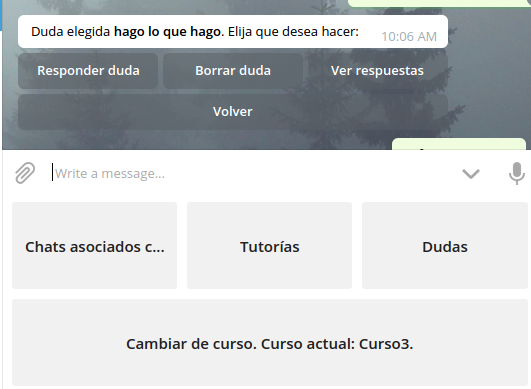
\includegraphics[scale=0.7]{imagenes/random/Screenshot_2017-08-21_13-09-40.png}  %el parámetro scale permite agrandar o achicar la imagen. En el nombre de archivo puede especificar directorios

\caption{Arriba menú tipo Inline, abajo menú tipo teclado}\label{figura10}
\end{figure}
Estos menús tienen la peculiaridad de que cuando un usuario pulsa una tecla  el bot recibe un mensaje tipo \enquote*{callback} (caso menús Inline) o de texto (menús tipo teclado) que identifica a la tecla pulsada dentro del menú.  Dicho lo cual, si se realiza un buen diseño de los menús, tanto el usuario como el bot pueden comprender perfectamente qué es lo que quiere el uno del otro.
\par
No se ha pensado en el uso de menús en los chats grupales porque pienso que generarían un ruido innecesario y que al ser interacciones \enquote*{de un solo paso} por parte del usuario son innecesarios.

\subsection{Diseño de la estructura}

Comenzamos a refinar el sistema para que éste empiece a estar lo suficientemente definido como para llevar a cabo su implementación. Hemos hablado brevemente del enrutamiento de mensajes en los CUs Reales y  en los diagramas anteriores hemos mostrado una clase \enquote*{pradobot} que es la encargada de conocer qué es lo que el usuario quiere y llevar a cabo las acciones pertinentes. Vamos a empezar a repartir las responsabilidades de dicha clase utilizando diferentes patrones de diseño. 
\subsubsection{Primera capa: controladores}

El bot es un programa que constantemente está escuchando por si Telegram le envía un nuevo mensaje y una vez recibido realiza una acción u otra.
Como hemos indicado en el apartado de diseño de interacción de usuario, la forma en que el bot se relaciona con un usuario entre un chat privado y uno grupal es muy diferente requiriendo la gestión de acciones que hacen uso de múltiples pasos mediante  menús para los usuarios de un chat privado ,mientras que las acciones que ejecutan los usuarios de los chats grupales solamente son de un paso y sin menús.

Esto nos lleva a aplicar el patrón \textbf{\enquote*{Controlador}} y distribuir las responsabilidades entre tres clases:
\begin{itemize}
\item \textbf{Mensajero}: su función es la de recibir mensajes, ver si proceden de un chat privado o grupal y transferir el mensaje a la clase responsable del manejo de mensajes procedentes de chats privados o a la de chats grupales.
\item \textbf{ManejadorMensajesChatsPrivados}: Recibe mensajes procedentes de un chat privado y lleva a cabo las siguientes funciones:
\begin{itemize}
\item Ver si el usuario que le habla está registrado en el sistema.
\item Controlar si el sistema ha acabado ya de procesar el último mensaje que le mandó el usuario.
\item Entregar el mensaje que le envía el usuario a una capa inferior para que ésta lleve a cabo una acción con el mensaje.
\end{itemize}
Esta clase no tiene la responsabilidad de ver qué se hace con el mensaje sino que lo transfiere a otra clase para que ésta lo procese.
\item \textbf{ManejadorMensajesChatsGrupales}: Recibe mensajes procedentes de un chat grupal. Sus funciones a destacar son:
\begin{itemize}
\item Controlar si los mensajes proceden de chats asociados a cursos del sistema.
\item Llevar a cabo el procesamiento del mensaje, lo cual desencadena en una acción.
\end{itemize}
Como  esta clase es la que conoce qué chat corresponde a qué curso y las interacciones con los chats grupales son tan básicas, se le ha asignado también la responsabilidad de ejecutar lo que quiere el usuario en el mensaje.
\end{itemize}

Podemos ver el funcionamiento de esta primera capa en las siguientes capturas:
\begin{figure}[H] %con el [H] le obligamos a situar aquí la figura
\centering
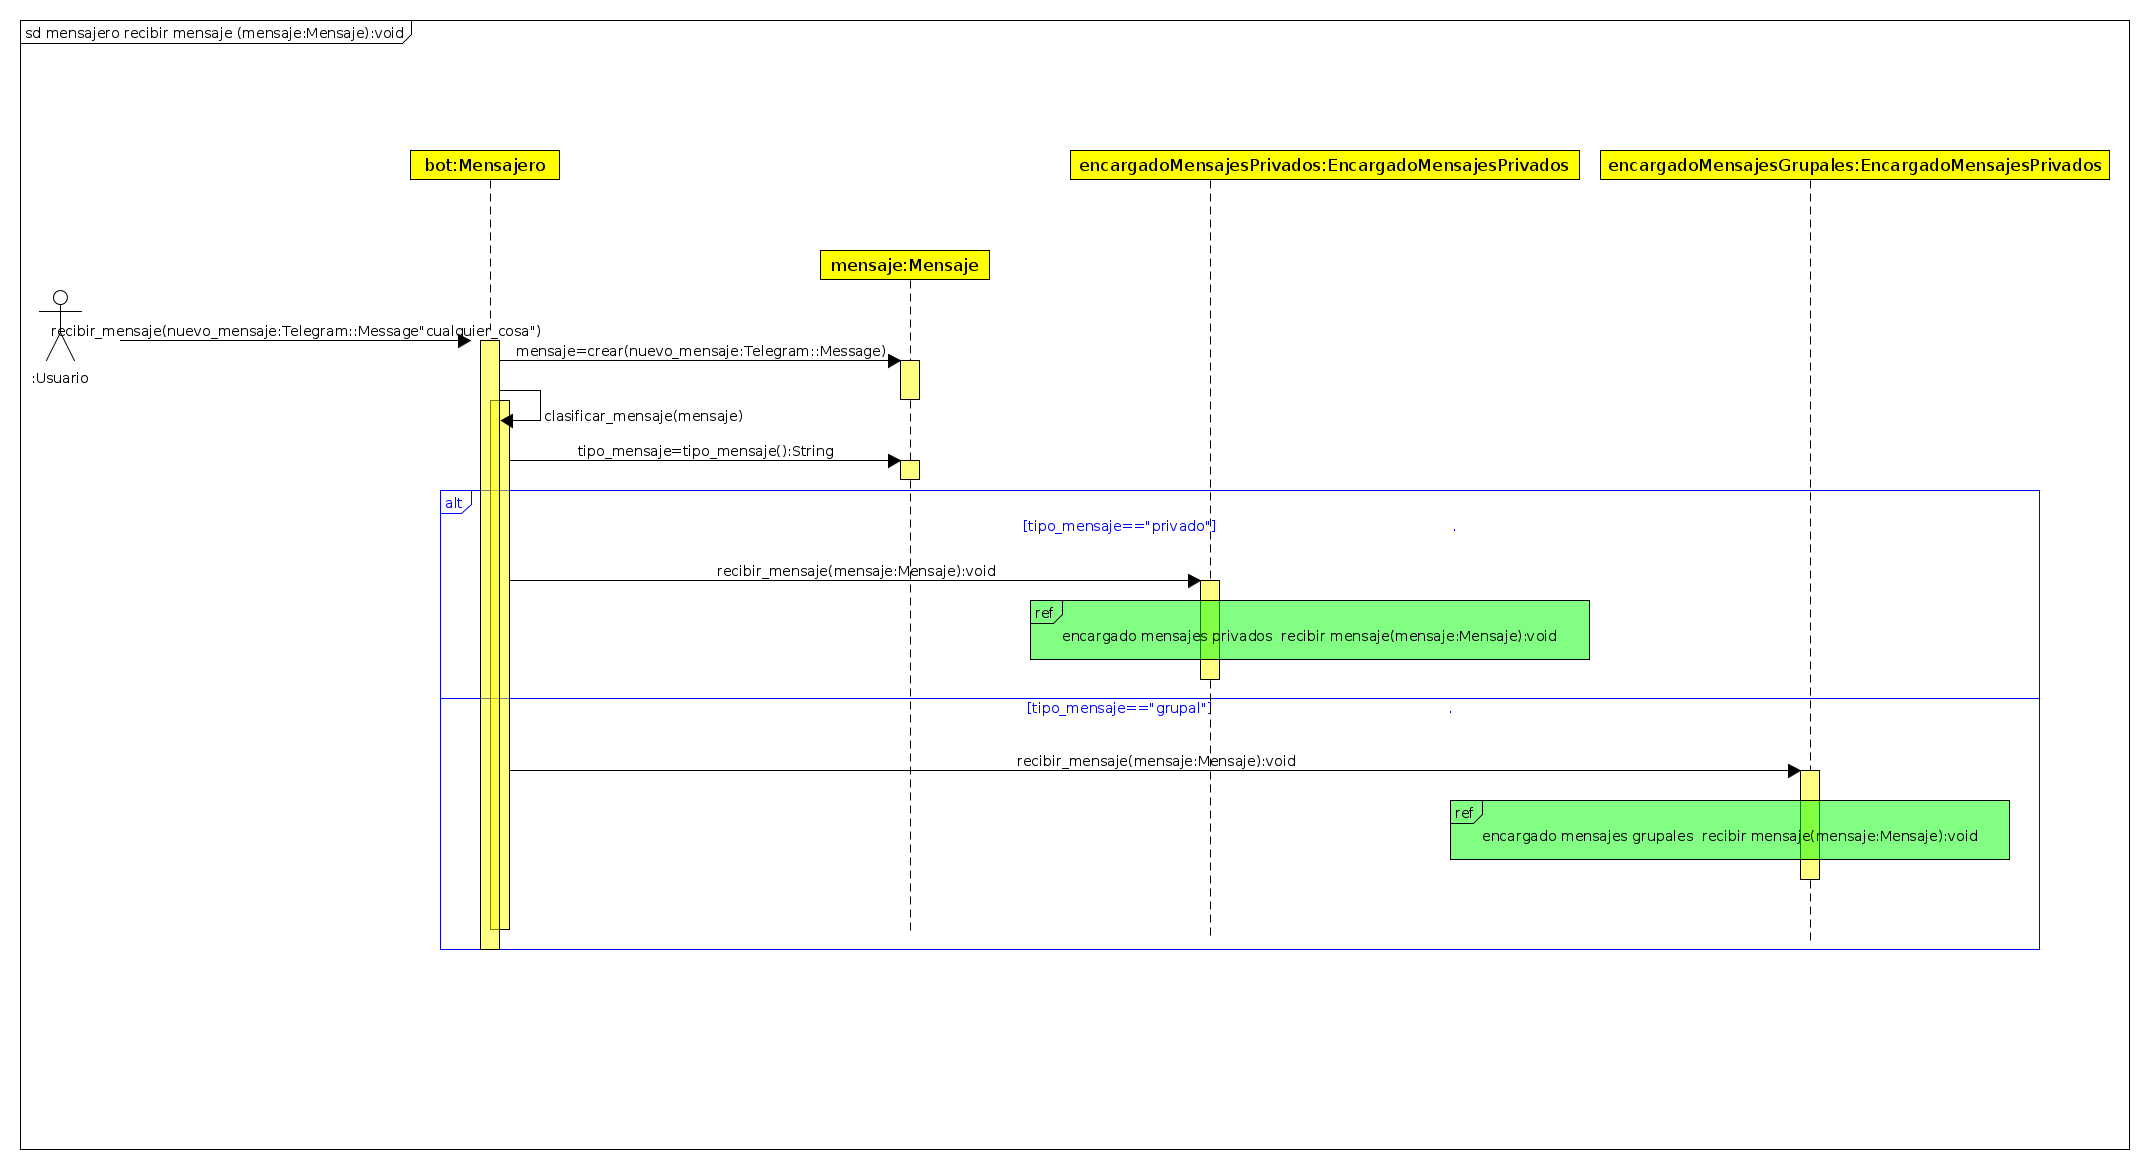
\includegraphics[scale=0.2]{imagenes/diagramas/secuencia/grandes/nuevo_mensaje.png}  %el parámetro scale permite agrandar o achicar la imagen. En el nombre de archivo puede especificar directorios

\caption{Diagrama secuencia recibir\_mensaje clase  Mensajero: el bot recibe un nuevo mensaje}\label{figura220}
\end{figure}

He preferido mostrar el funcionamiento de como opera el ManejadorMensajesPrivados debido a que es bastante más complejo que el de chats grupales:


\begin{figure}[H] %con el [H] le obligamos a situar aquí la figura
\centering
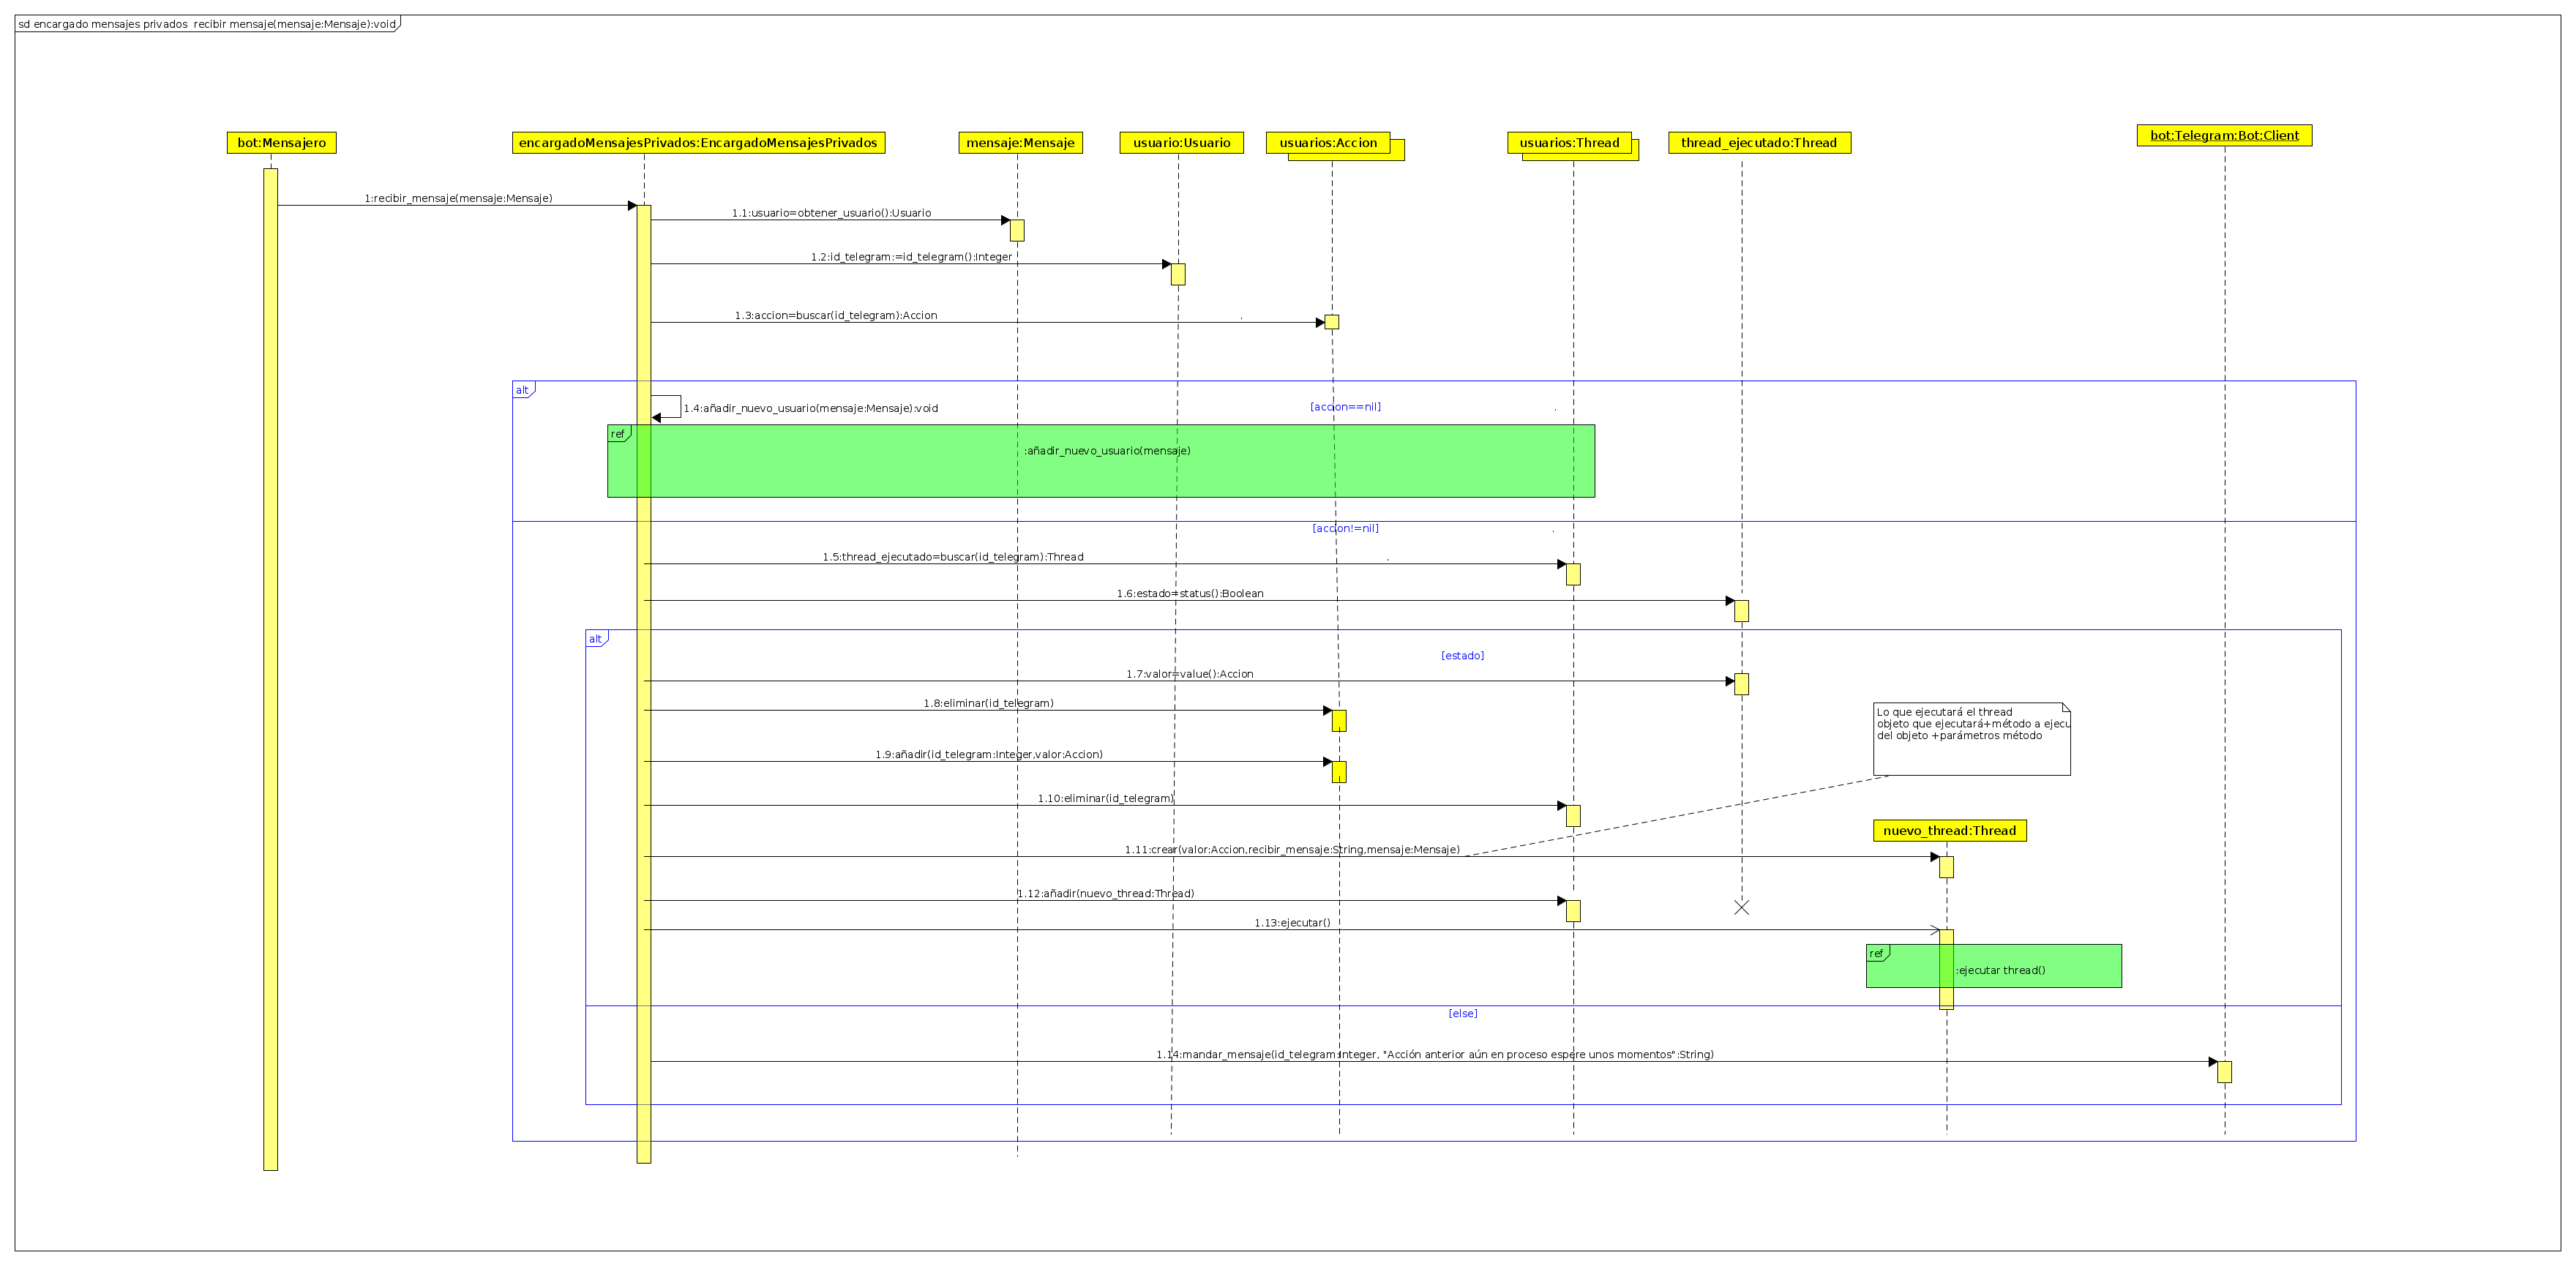
\includegraphics[scale=0.12]{imagenes/diagramas/secuencia/grandes/clasificar_mensaje_comprimido.png}  %el parámetro scale permite agrandar o achicar la imagen. En el nombre de archivo puede especificar directorios

\caption{Diagrama secuencia recibir\_mensaje clase  ManejadorMensajesChatsPrivados}\label{figura221}
\end{figure}




\begin{figure}[H] %con el [H] le obligamos a situar aquí la figura
\centering
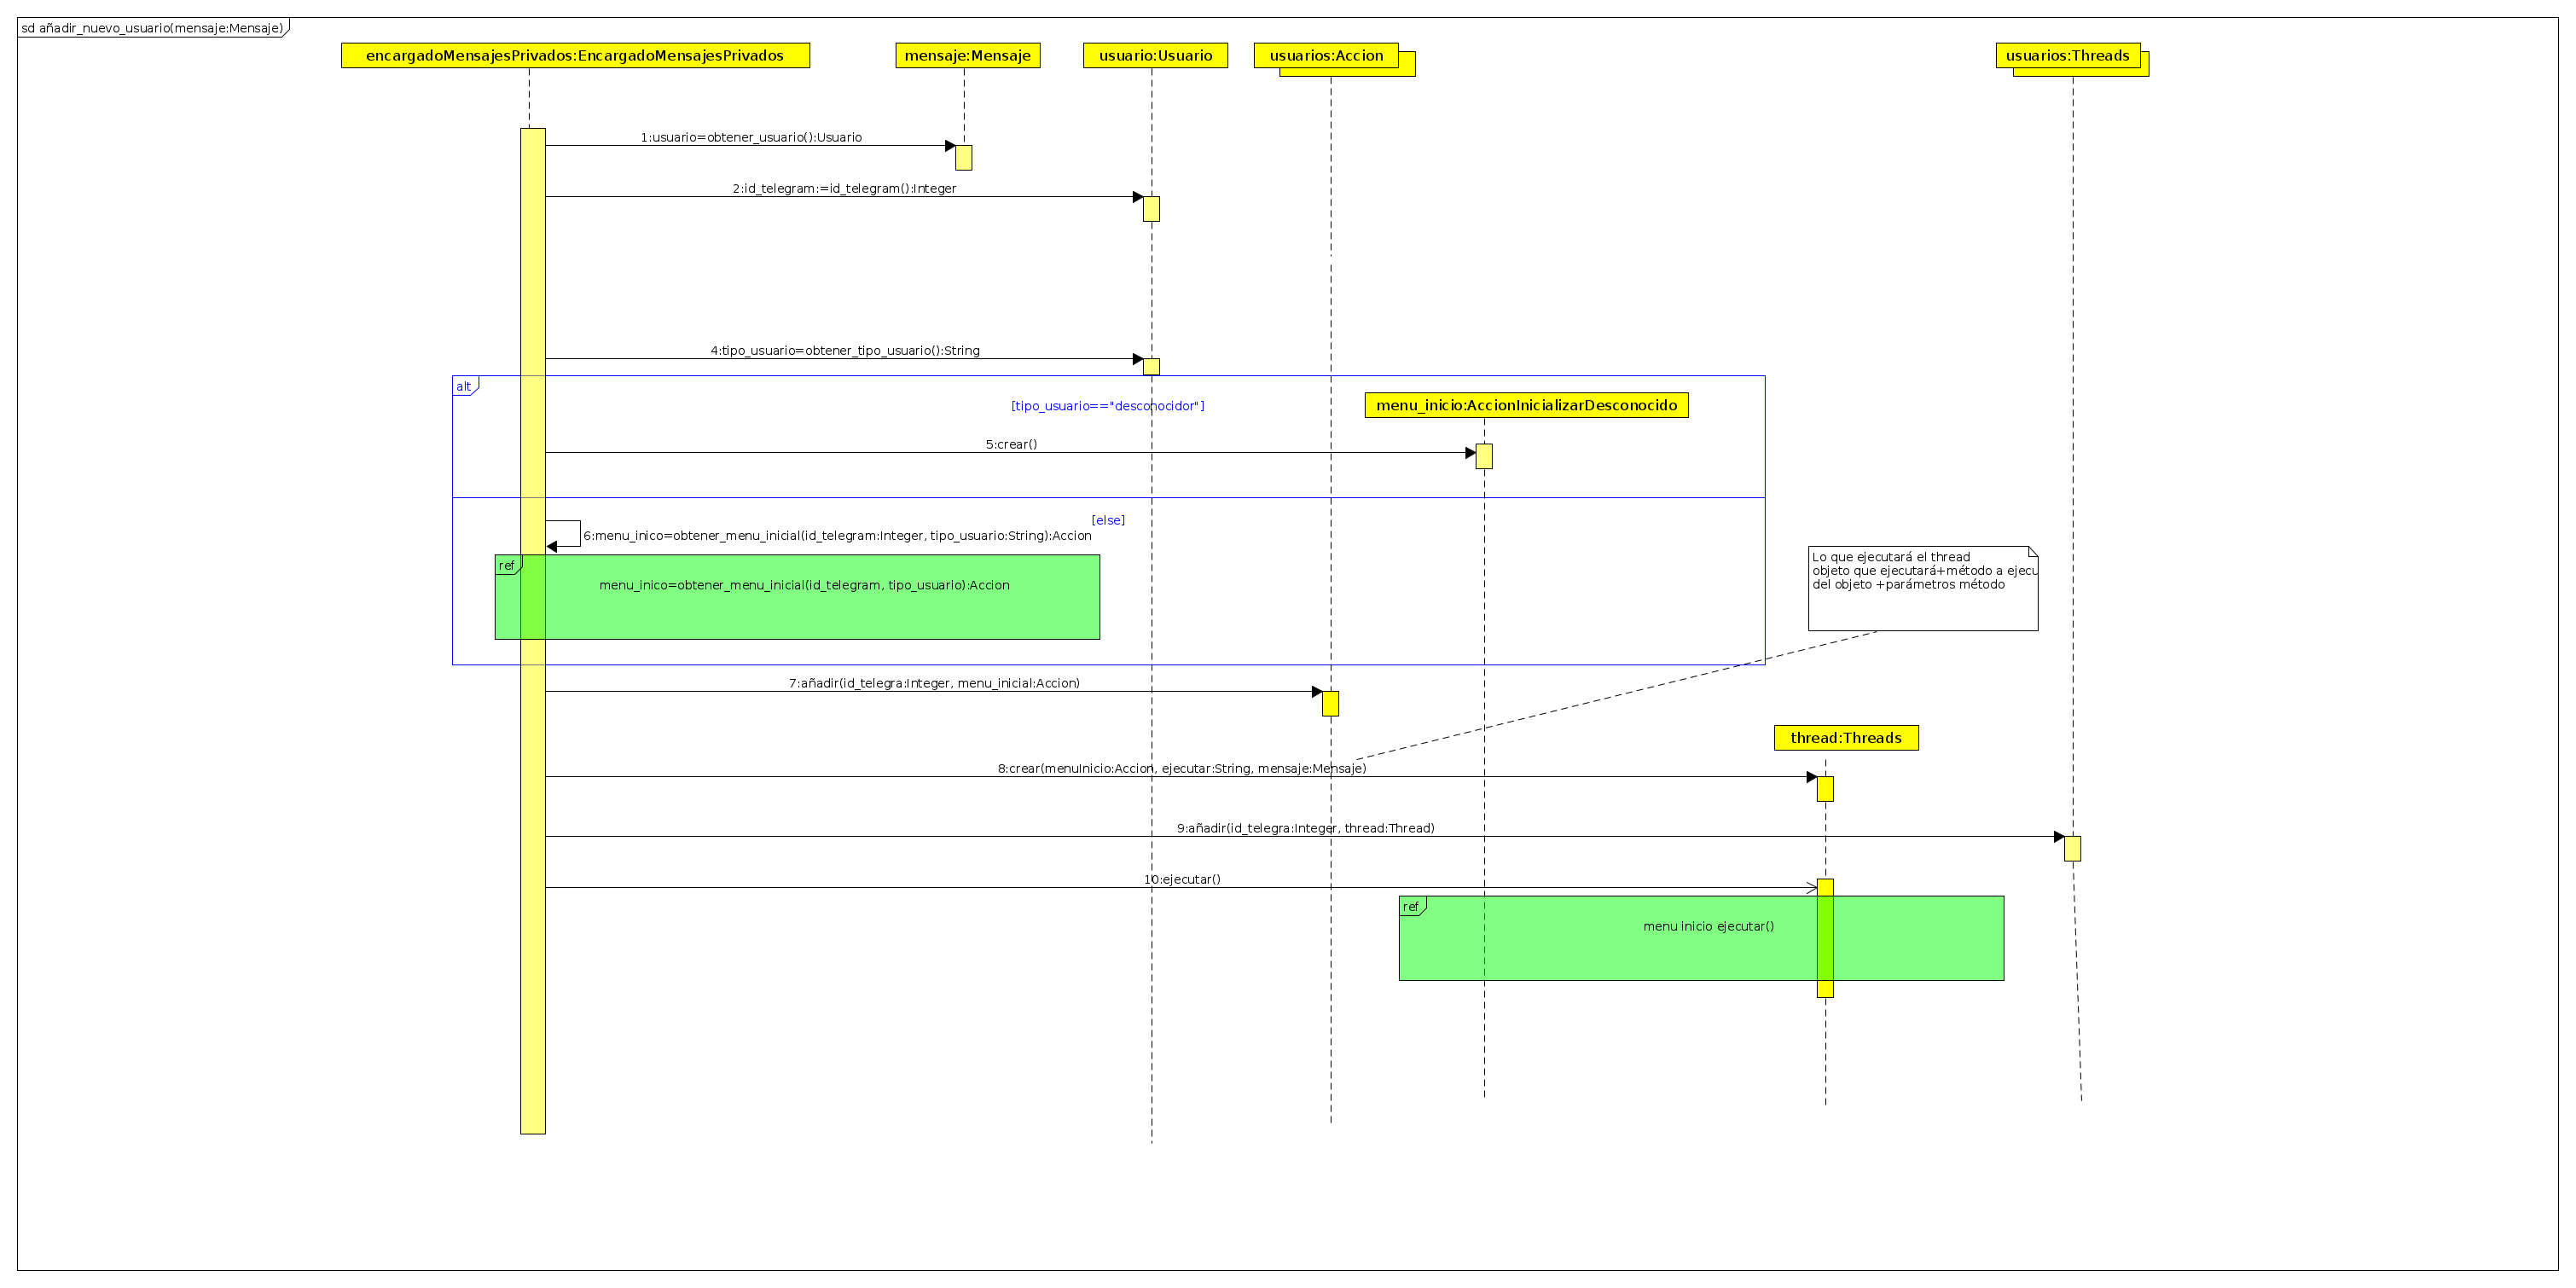
\includegraphics[scale=0.14]{imagenes/diagramas/secuencia/grandes/anadir_nuevo_usuario.png}  %el parámetro scale permite agrandar o achicar la imagen. En el nombre de archivo puede especificar directorios

\caption{Diagrama secuencia añadir\_nuevo\_usuario clase  ManejadorMensajesChatsPrivados}\label{figura222}
\end{figure}


\begin{figure}[H] %con el [H] le obligamos a situar aquí la figura
\centering
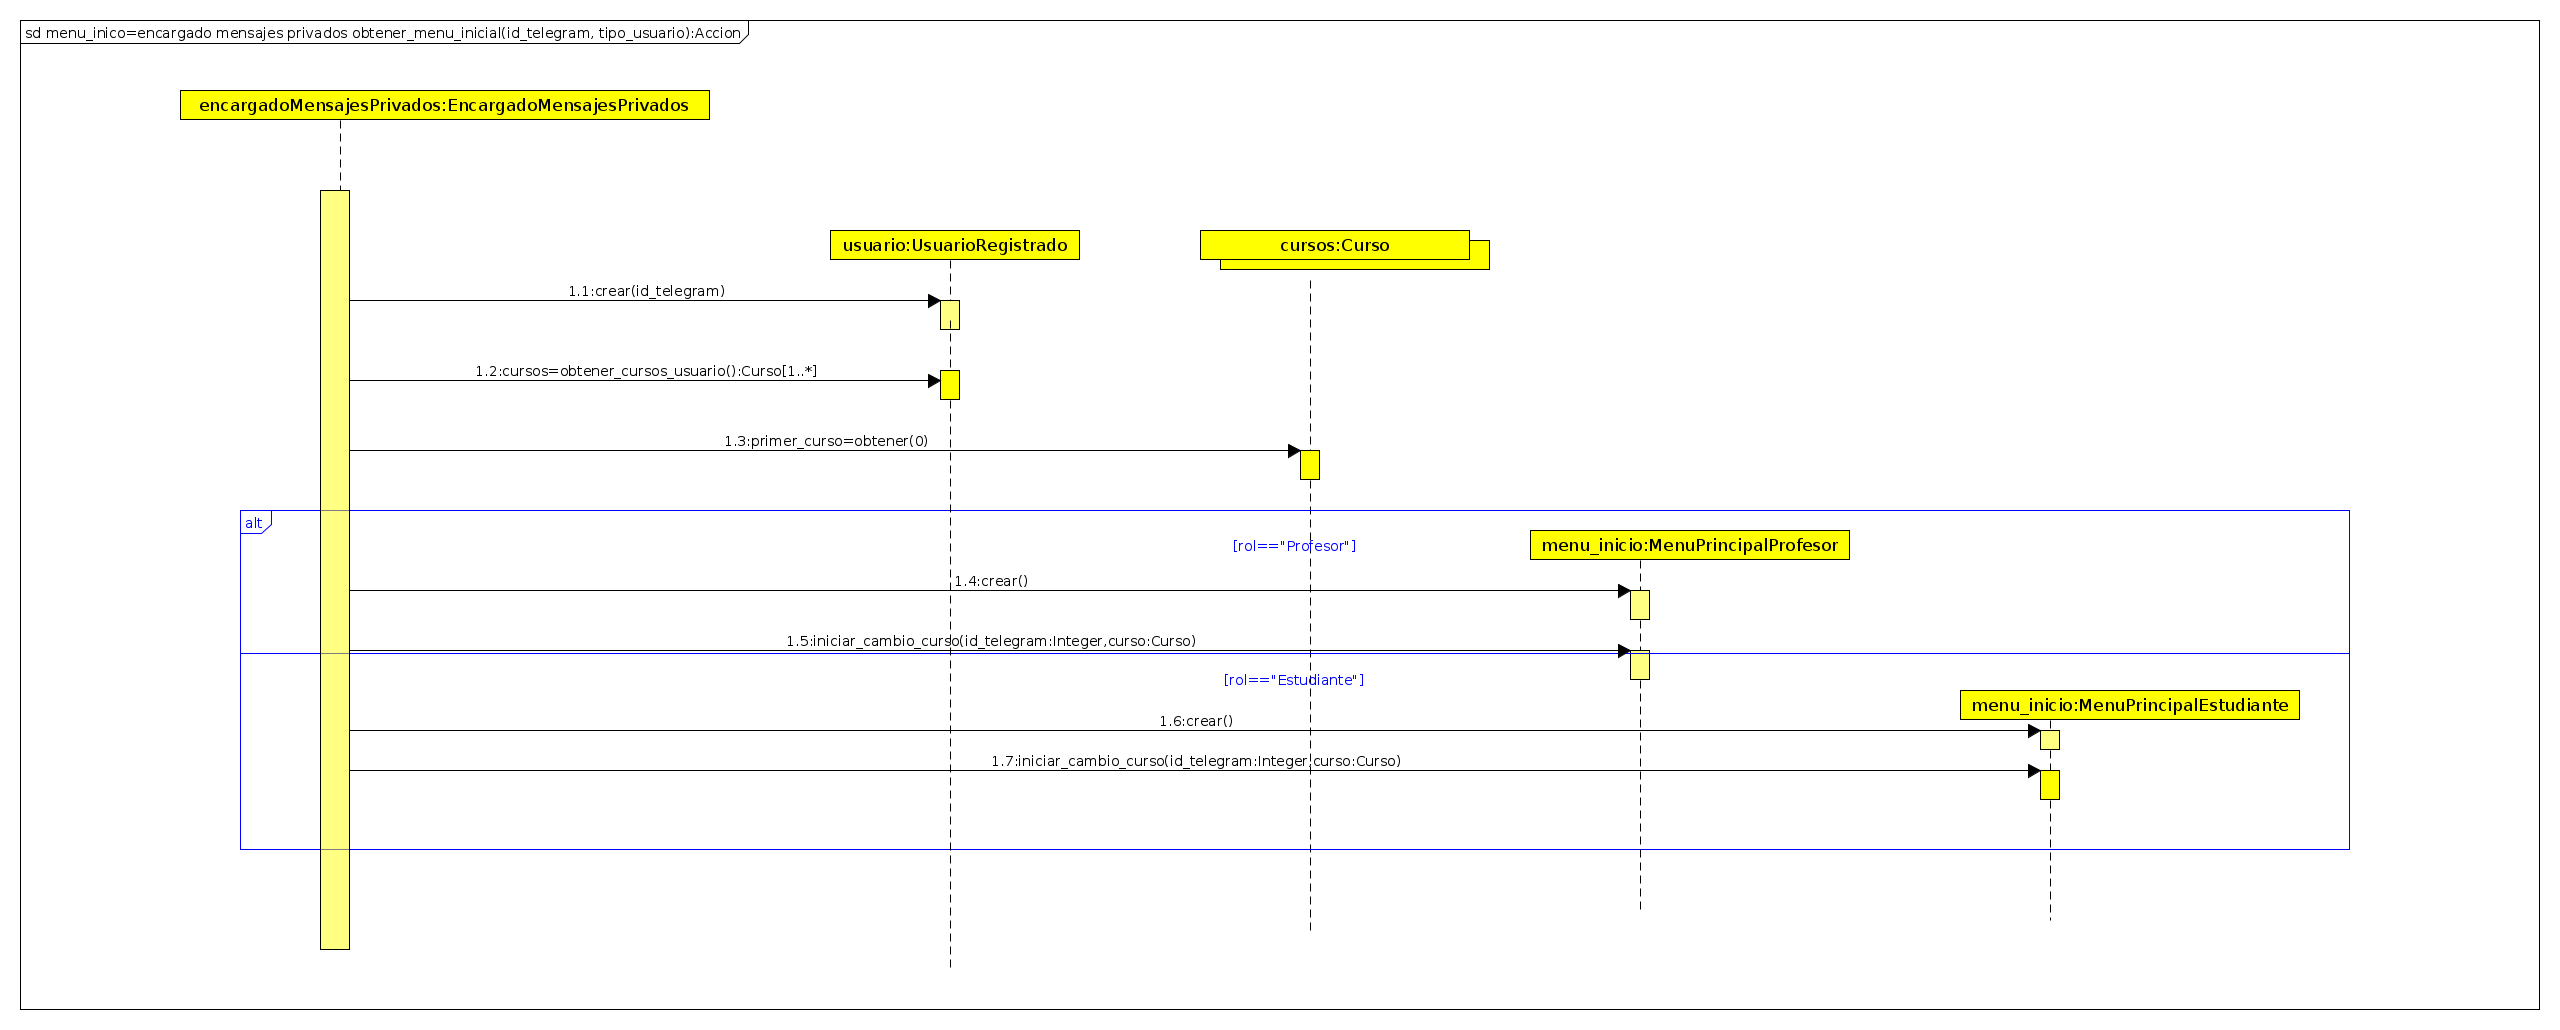
\includegraphics[scale=0.16]{imagenes/diagramas/secuencia/grandes/obtener_menu_inicio.png}  %el parámetro scale permite agrandar o achicar la imagen. En el nombre de archivo puede especificar directorios

\caption{Diagrama secuencia obtener\_menu\_inicio clase  ManejadorMensajesChatsPrivados}\label{figura223}
\end{figure}

\begin{figure}[H] %con el [H] le obligamos a situar aquí la figura
\centering
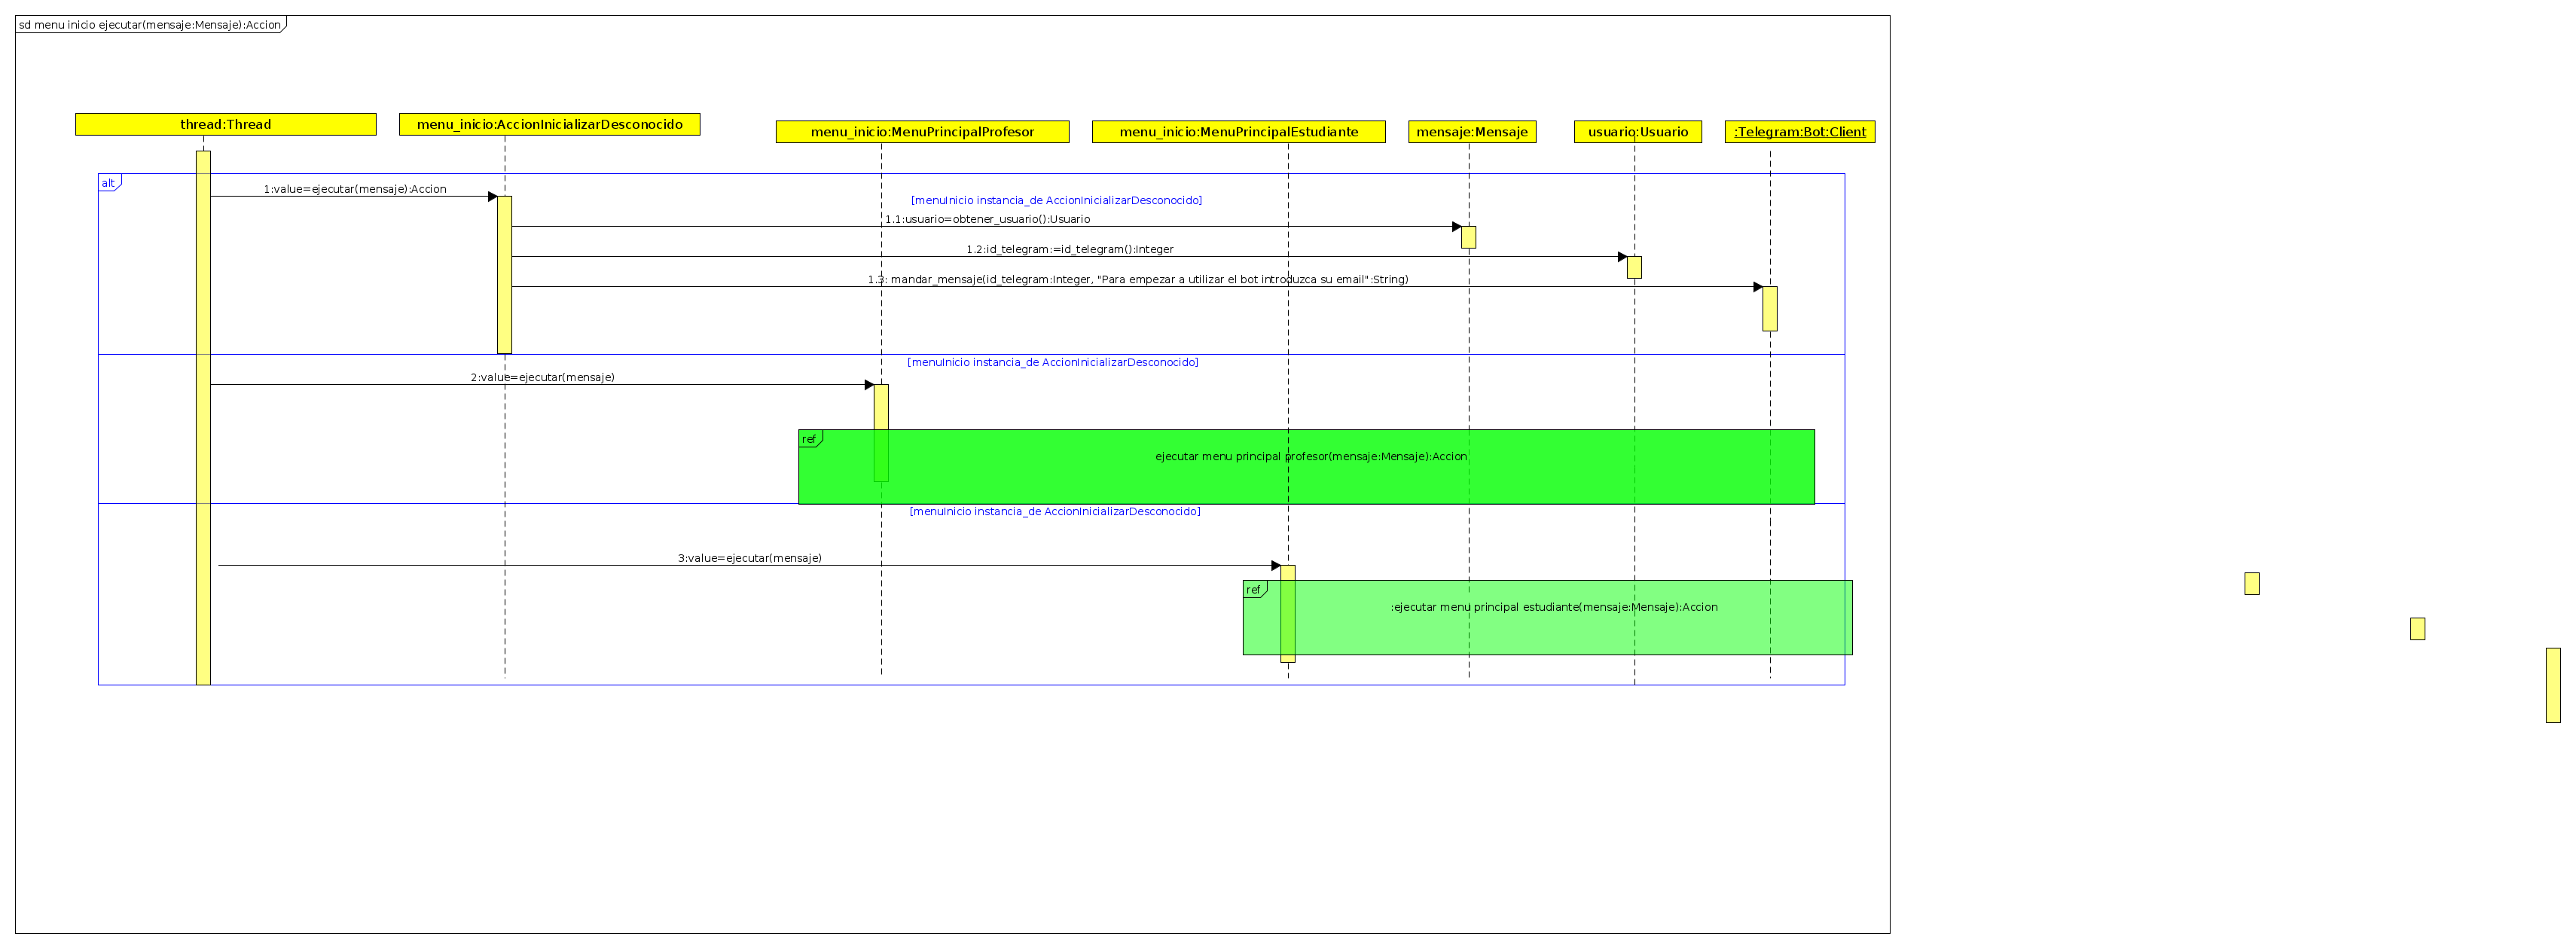
\includegraphics[scale=0.16]{imagenes/diagramas/secuencia/grandes/menu_inicio_ejecutar.png}  %el parámetro scale permite agrandar o achicar la imagen. En el nombre de archivo puede especificar directorios

\caption{Diagrama secuencia ejecutar\_menu\_inicio clase  ManejadorMensajesChatsPrivados}\label{figura227}
\end{figure}

En la siguiente captura se puede apreciar el polimorfismo. Explciaremos su uso en el programa en la siguiente sección.

\begin{figure}[H] %con el [H] le obligamos a situar aquí la figura
\centering
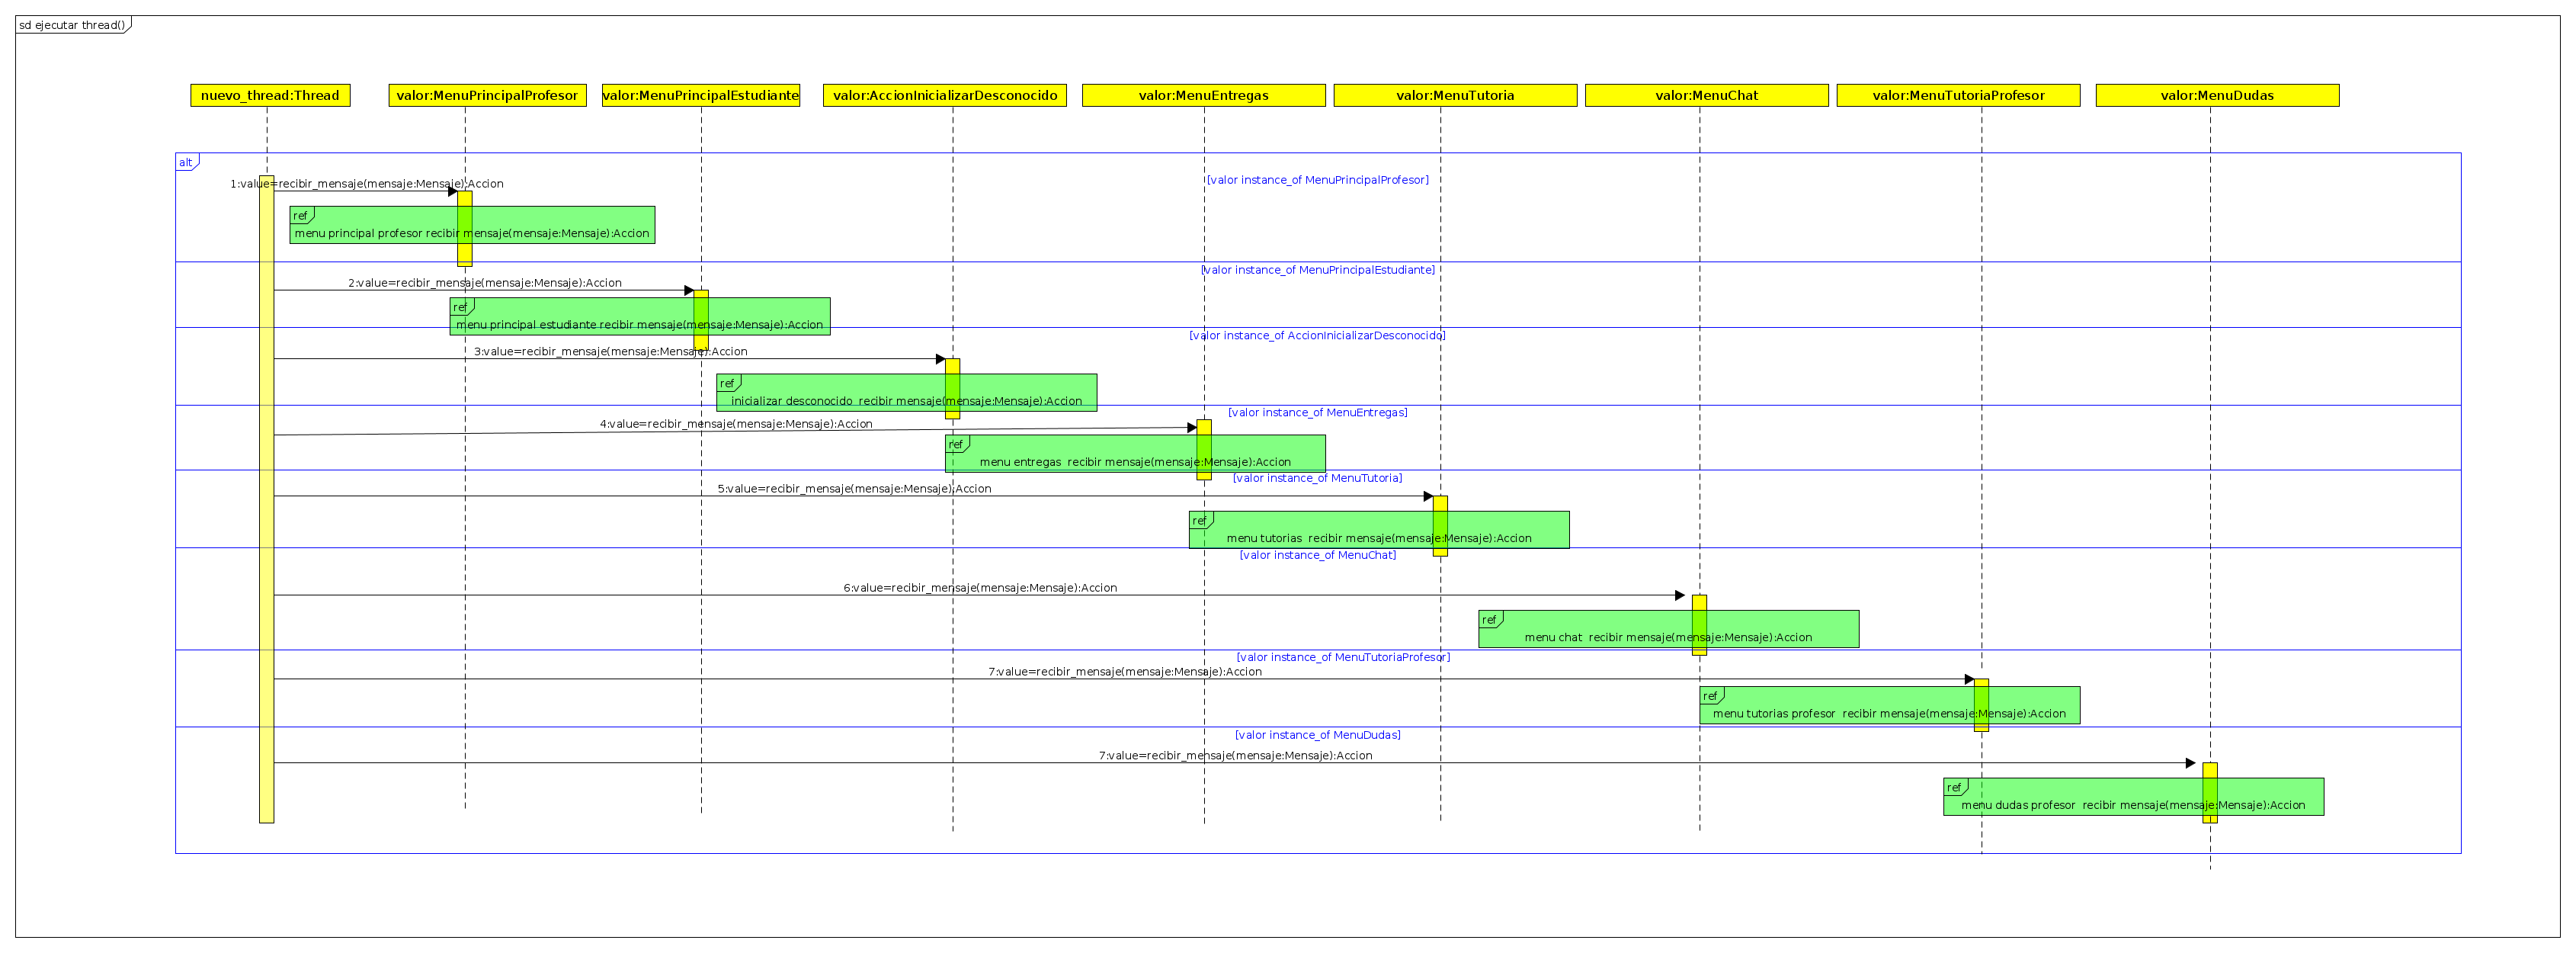
\includegraphics[scale=0.13]{imagenes/diagramas/secuencia/grandes/ejecutar_thread.png}  %el parámetro scale permite agrandar o achicar la imagen. En el nombre de archivo puede especificar directorios

\caption{Diagrama secuencia muestra ejecución thread iniciado por ManejadorMensajesChatsPrivados }\label{figura223}
\end{figure}
\subsubsection*{Segunda capa: menús}


\textbf{ManejadorMensajesChatsPrivados} le pasa el mensaje a otra clase que es la encargada de ver qué quiere el usuario con el mensaje. 
 Debido al diseño mediante menús que se ha decidido hacer  para interaccionar con el usuario, la clase que realmente sabe qué es lo que quiere hacer el usuario con su mensaje es aquella que controla al menú que está viendo el usuario ya que ésta es la que conoce las opciones contenidas en el menú. El mensaje que recibe un menú puede indicar tres cosas:
\begin{itemize}
\item Selección de una nueva opción del menú.
\item Indicar que se quiere cambiar de menú.
\item El mensaje no está destinado al menú sino a la última opción que pulsó el usuario en el menú.
\end{itemize} 
 
 El procesamiento de un mensaje por parte de una clase menú siempre devuelve otra clase menú que será la que reciba el proximo mensaje de ManejadorMensajesChatsPrivados. Puede devolverse a ella misma o a su menú padre. He aquí el \textbf{Polimorfismo}.
 La jerarquía de menús puede descomponerse en:
 
 \begin{itemize}
 \item MenuPrincipalEstudiante: El menú que vé un estudiante la primera vez que le manda un mensaje al bot. Contiene:
 \begin{itemize}
 \item MenuTutorias
 \item MenuEntregas
 \item MenuDudas
 \end{itemize}
 \item MenuPrincipalProfesor: Igual que el menú anterior pero para el profesor. Contiene:
 \begin{itemize}
 \item MenuTutoriasProfesor
 \item MenuChatTelegram
 \item MenuDudas
 \end{itemize}
\item MenuTutoriasProfesor: Contiene las opciones:
\begin{itemize}
\item Ver cola de tutorías
\item Crear tutoría
\item Borrar tutoría.
\end{itemize}
\item MenuChatTelegram: Contiene las opciones:
\begin{itemize}
\item Asociar curso a chat.
\end{itemize}
\item MenuTutorias: Permite al estudiante elegir entre:
\begin{itemize}
\item Solicitar asistencia tutoría.
\item Ver estado de sus solicitudes.
\end{itemize}
\item MenuEntregas: Permite al estudiante:
\begin{itemize}
\item Obtener información de próximas entregas.
\item Ver calificaciones.
\end{itemize}
\item MenuDudas: contiene las opciones: 
\begin{itemize}
\item Crear duda.
\item Opción que permite: 
\begin{itemize}
\item Ver dudas con solución.
\item Ver dudas sin solución.
\item Ver dudas del usuario.
\item Ver respuestas dudas.
\item Seleccionar una respuesta como solución a duda.
\item Borrar duda.
\end{itemize}
 \end{itemize}
\end{itemize}

La jerarquía de menús se ha diseñado con especial énfasis en que las acciones que realizan algo similar estén contenidas en el mismo menú. Aquellas opciones que permiten más de una opción han sido anidadas así para evitar la repetición de acciones por parte de un usuario. Ejemplo:\par
Si un usuario selecciona una duda se le muestre que puede borrar la duda, ver sus respuestas, asignarle una solución... y no al revés, es decir,  tener un menú con la opción borrar duda, ver respuestas, asignarle solución y que nada más pulsar cualquiera de ellas te solicite que elijas la duda.
\par
Todos los menús, además, contienen la opción de cambiar de curso y  la de volver al menú anterior (menos los menús principales ya que no tienen menú anterior).





\subsubsection{Tercera capa: opciones de menús}


Cada opción de un menú está representada por una clase, que es la que conoce los pasos que tiene que realizar un usuario para llevar a cabo la acción que representa, así como de mediar entre el usuario y los \enquote*{objetos} que intervienen en esa acción. Recibe los mensajes procedentes del menú que la contiene y de ellos extrae la información que necesita.


\subsubsection{Cuarta capa: contenedores de datos}
El objetivo de las clases de esta capa es la de hacer de árbitro entre los datos ( Moodle y la base de datos) y el resto del sistema. Son las únicas que utilizan la API de Moodle cuando es necesario y hacen llamadas a la base de datos cuando se les solicita un dato de la clase que simbolizan (ejemplo: dudas creadas por un usuario).

Para ilustrar las interacciones entre la tercera y cuarta capas podemos ver el siguiente diagrama de comunicación de la opción solicitar tutoría que recibe mensaje de menú MenuTutorias:


\begin{figure}[H] %con el [H] le obligamos a situar aquí la figura
\centering
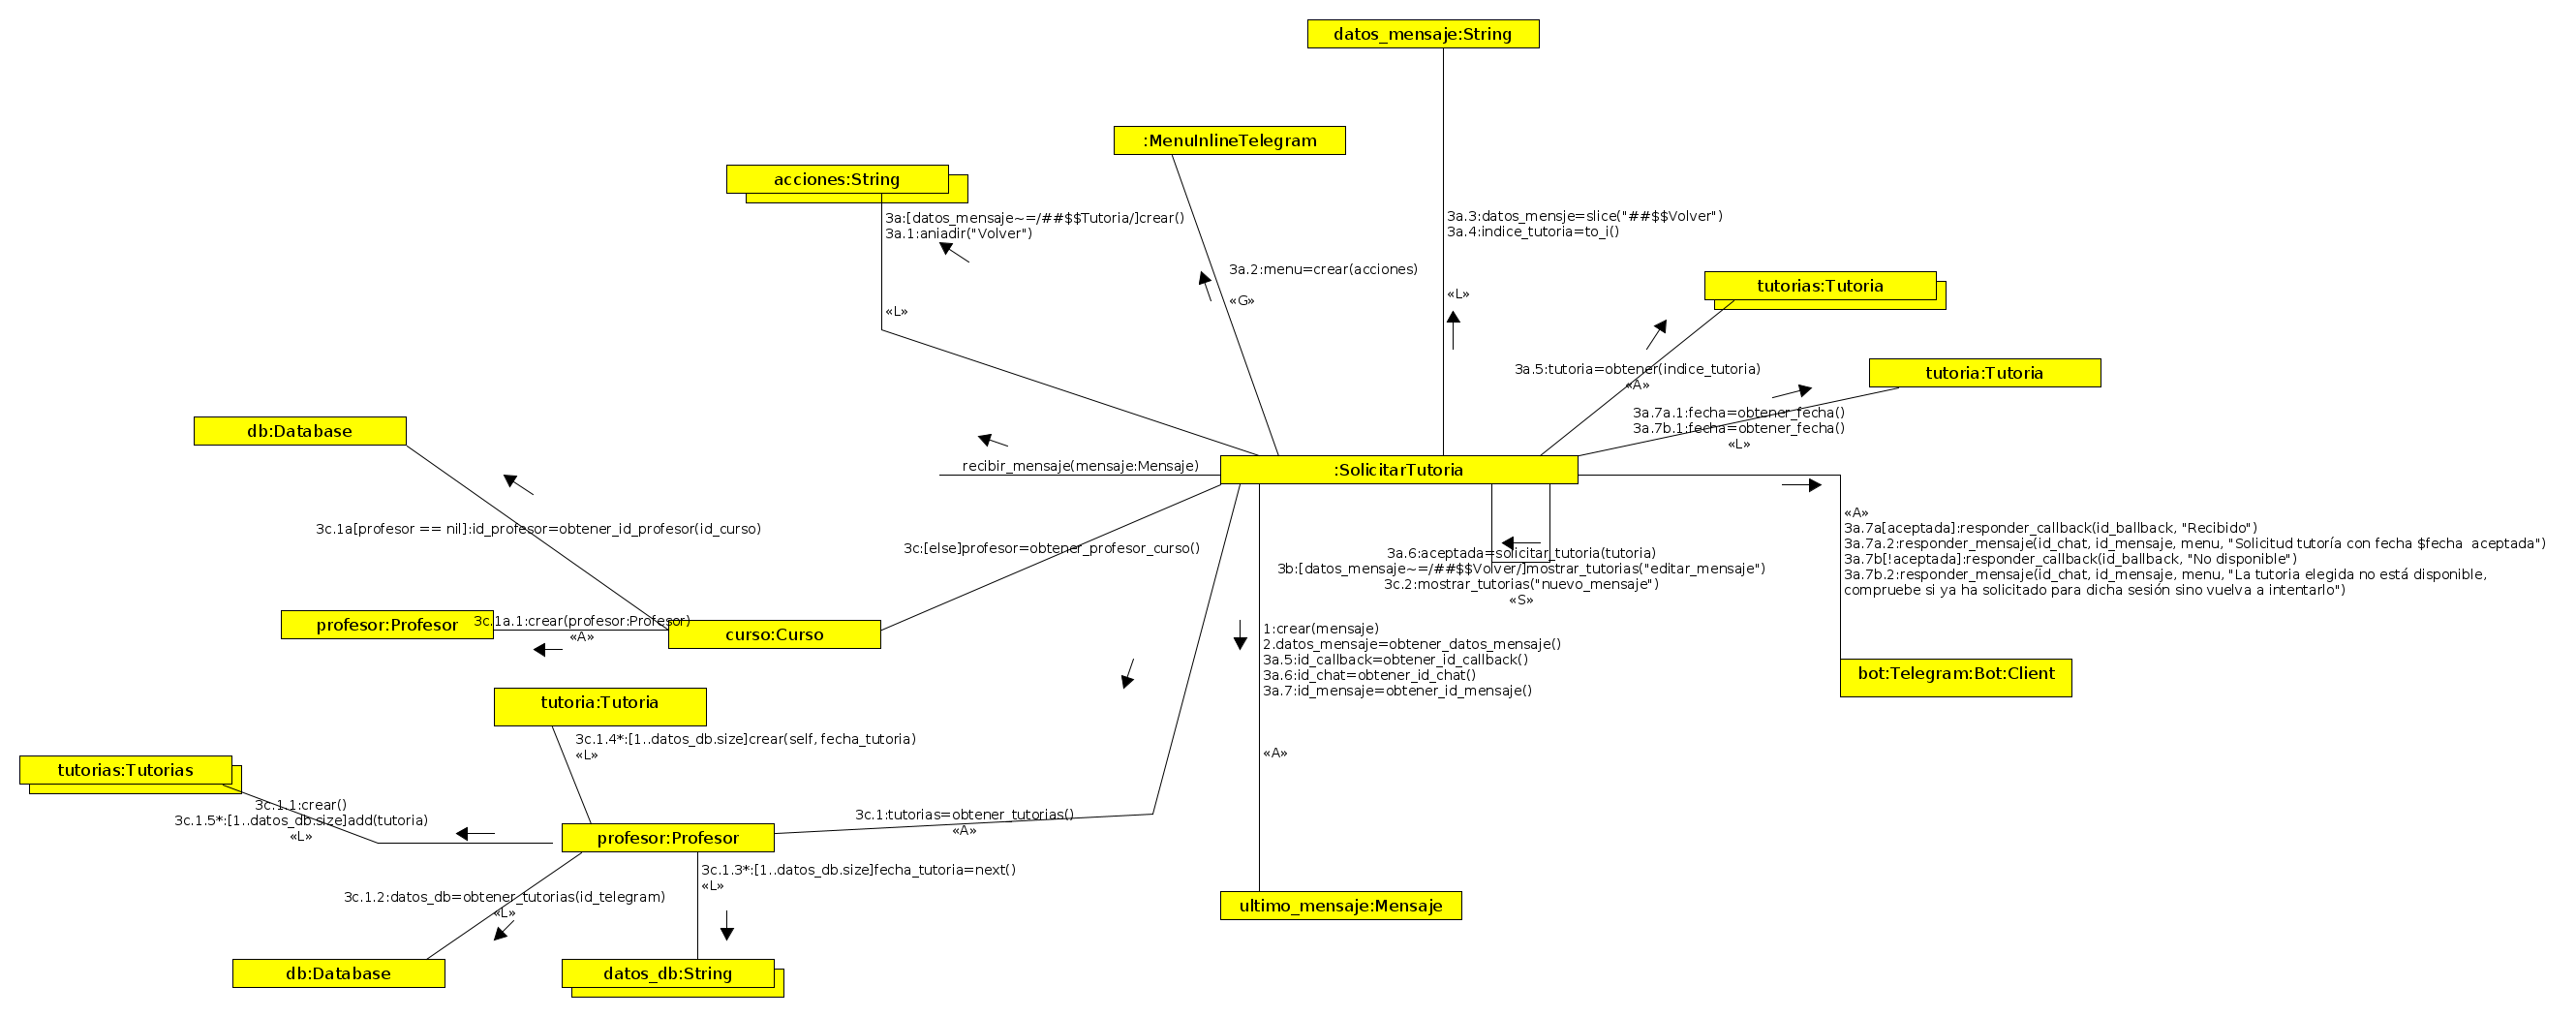
\includegraphics[scale=0.18]{imagenes/diagramas/comunicacion/solicitar_tutoria_recibir_mensaje.png}  %el parámetro scale permite agrandar o achicar la imagen. En el nombre de archivo puede especificar directorios

\caption{Diagrama comunicación recibir\_mensaje clase  SolicitarTutoria}\label{figura110}
\end{figure}

En el diagrama se puede observar como la clase SolicitarTutoria crea y envía diferentes mensajes al usuario empleando para el contenido de estos información de las clases Profesor y Tutoría.


\begin{figure}[H] %con el [H] le obligamos a situar aquí la figura
\centering
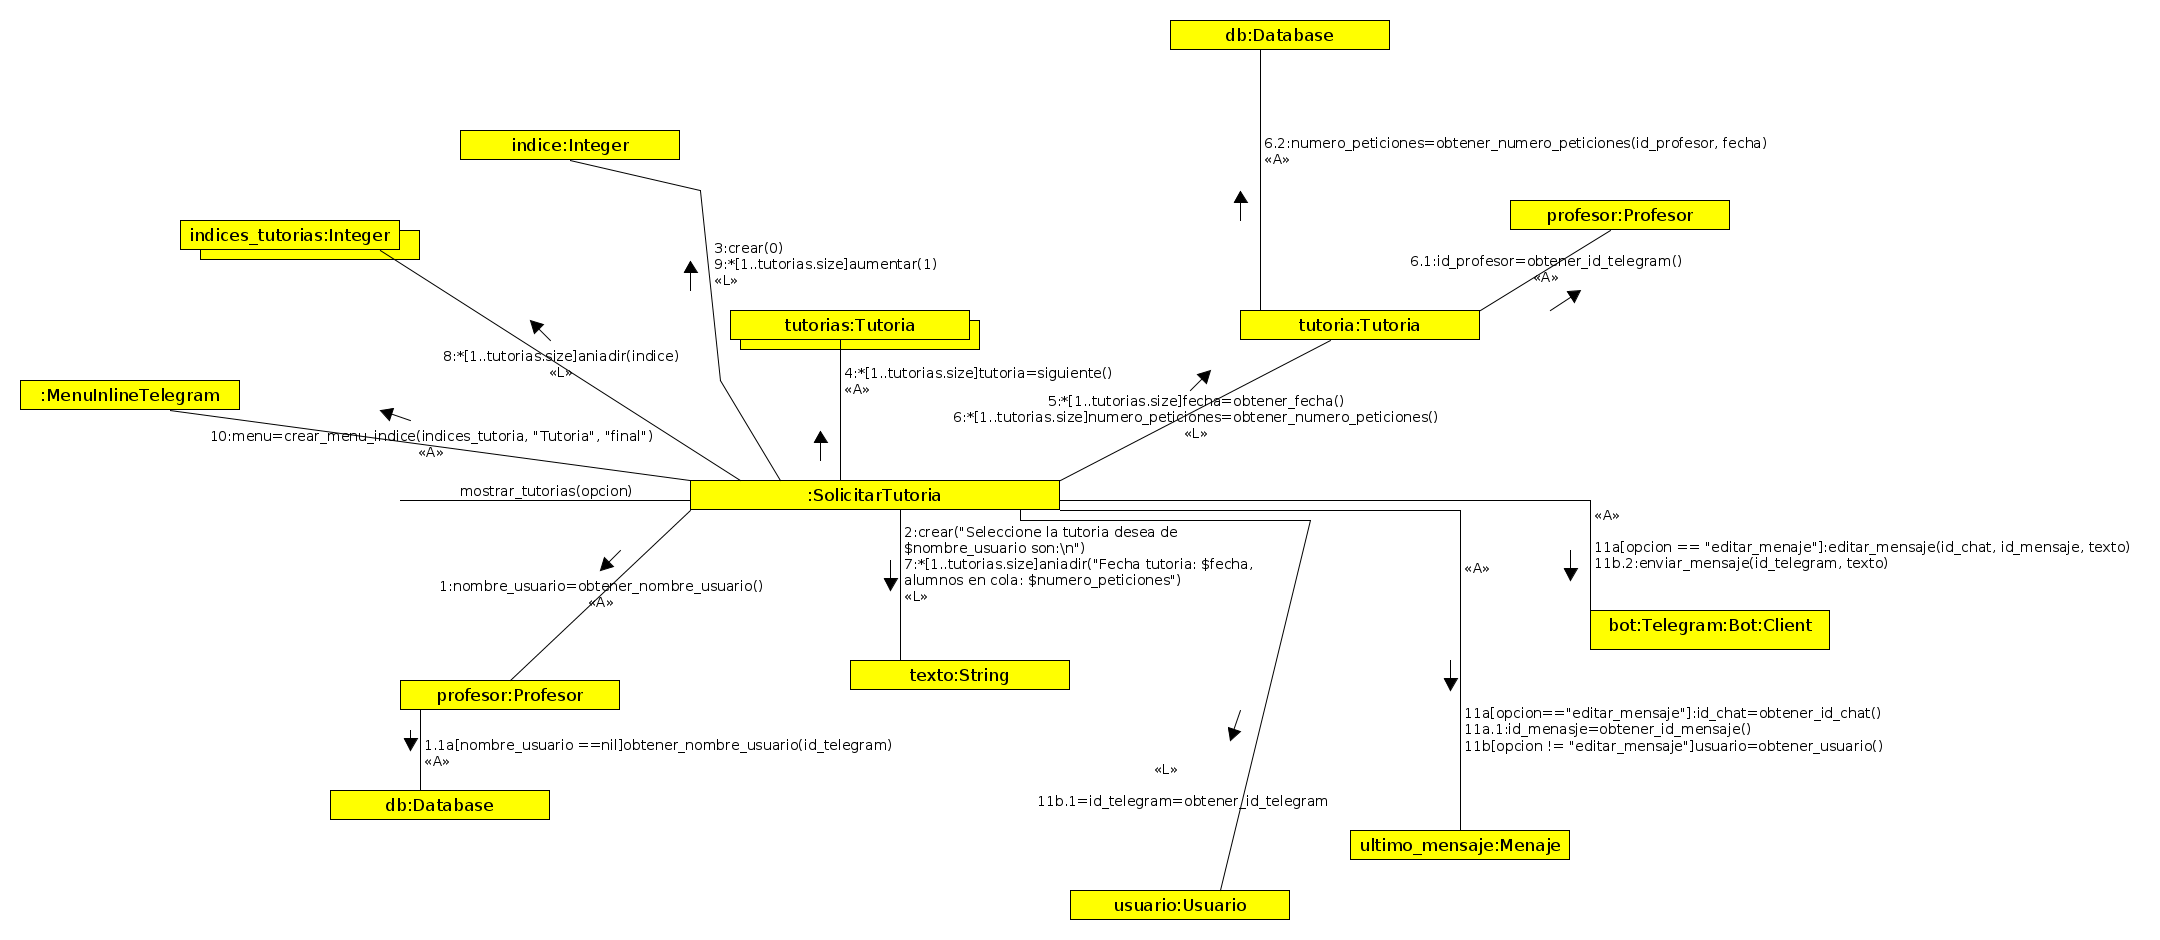
\includegraphics[scale=0.2]{imagenes/diagramas/comunicacion/mostrar_tutorias.png}  %el parámetro scale permite agrandar o achicar la imagen. En el nombre de archivo puede especificar directorios

\caption{Diagrama comunicación mostrar\_tutorías clase  SolicitarTutoria}\label{figura111}
\end{figure}


\begin{figure}[H] %con el [H] le obligamos a situar aquí la figura
\centering
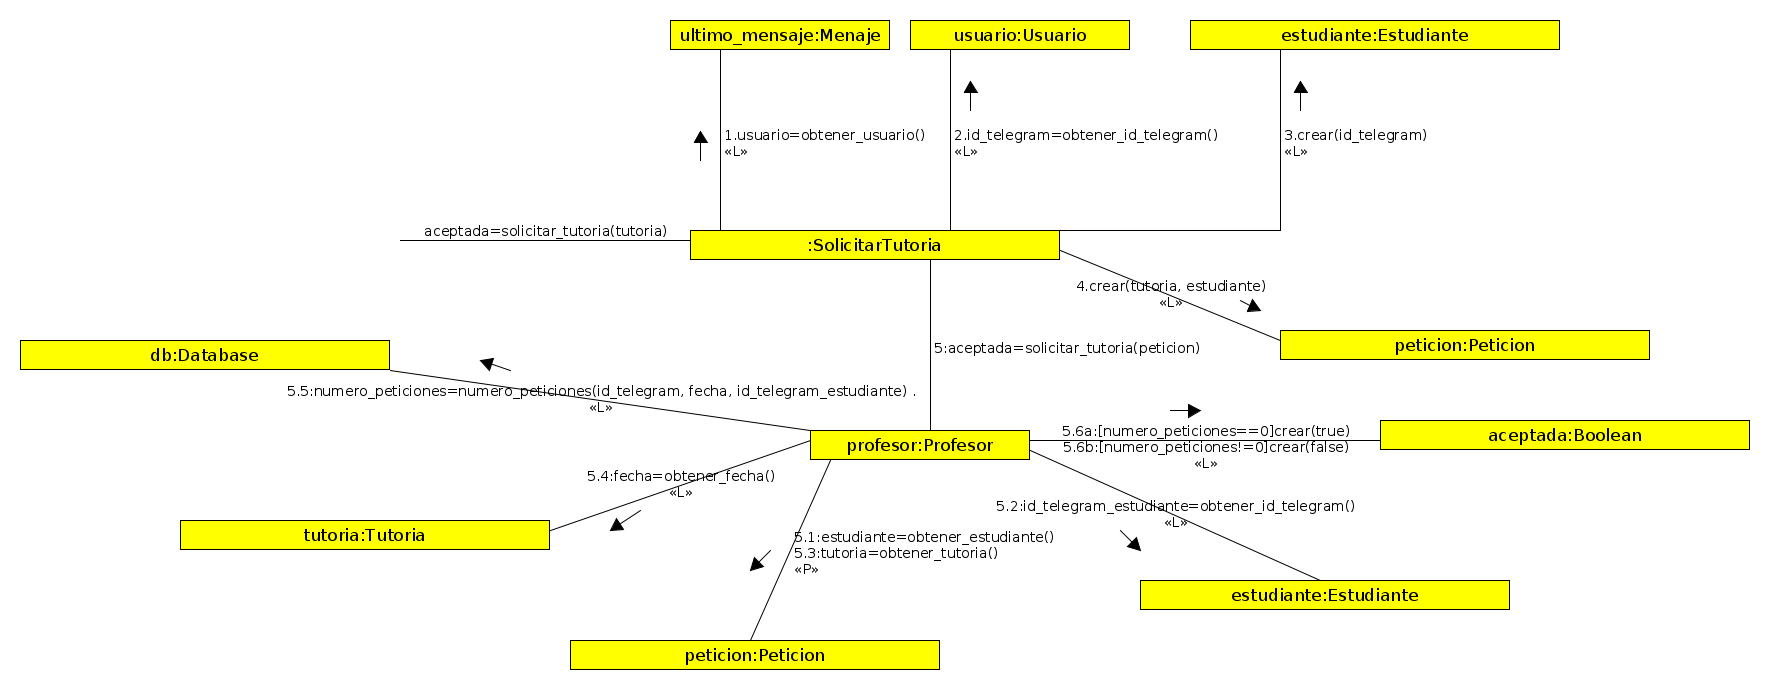
\includegraphics[scale=0.2]{imagenes/diagramas/comunicacion/solicitar_tutoria_tutoria.png}  %el parámetro scale permite agrandar o achicar la imagen. En el nombre de archivo puede especificar directorios

\caption{Diagrama comunicación solicitar\_tutoria clase  SolicitarTutoria}\label{figura112}
\end{figure}

El diagrama de clases obtenido al final para la aplicación sale demasiado grande para que sea fácilmente visible en el pdf. Se puede encontrar dentro de la carpeta diagramas con el nombre diagrama\_clases.png.

 \begin{figure}[H] %con el [H] le obligamos a situar aquí la figura
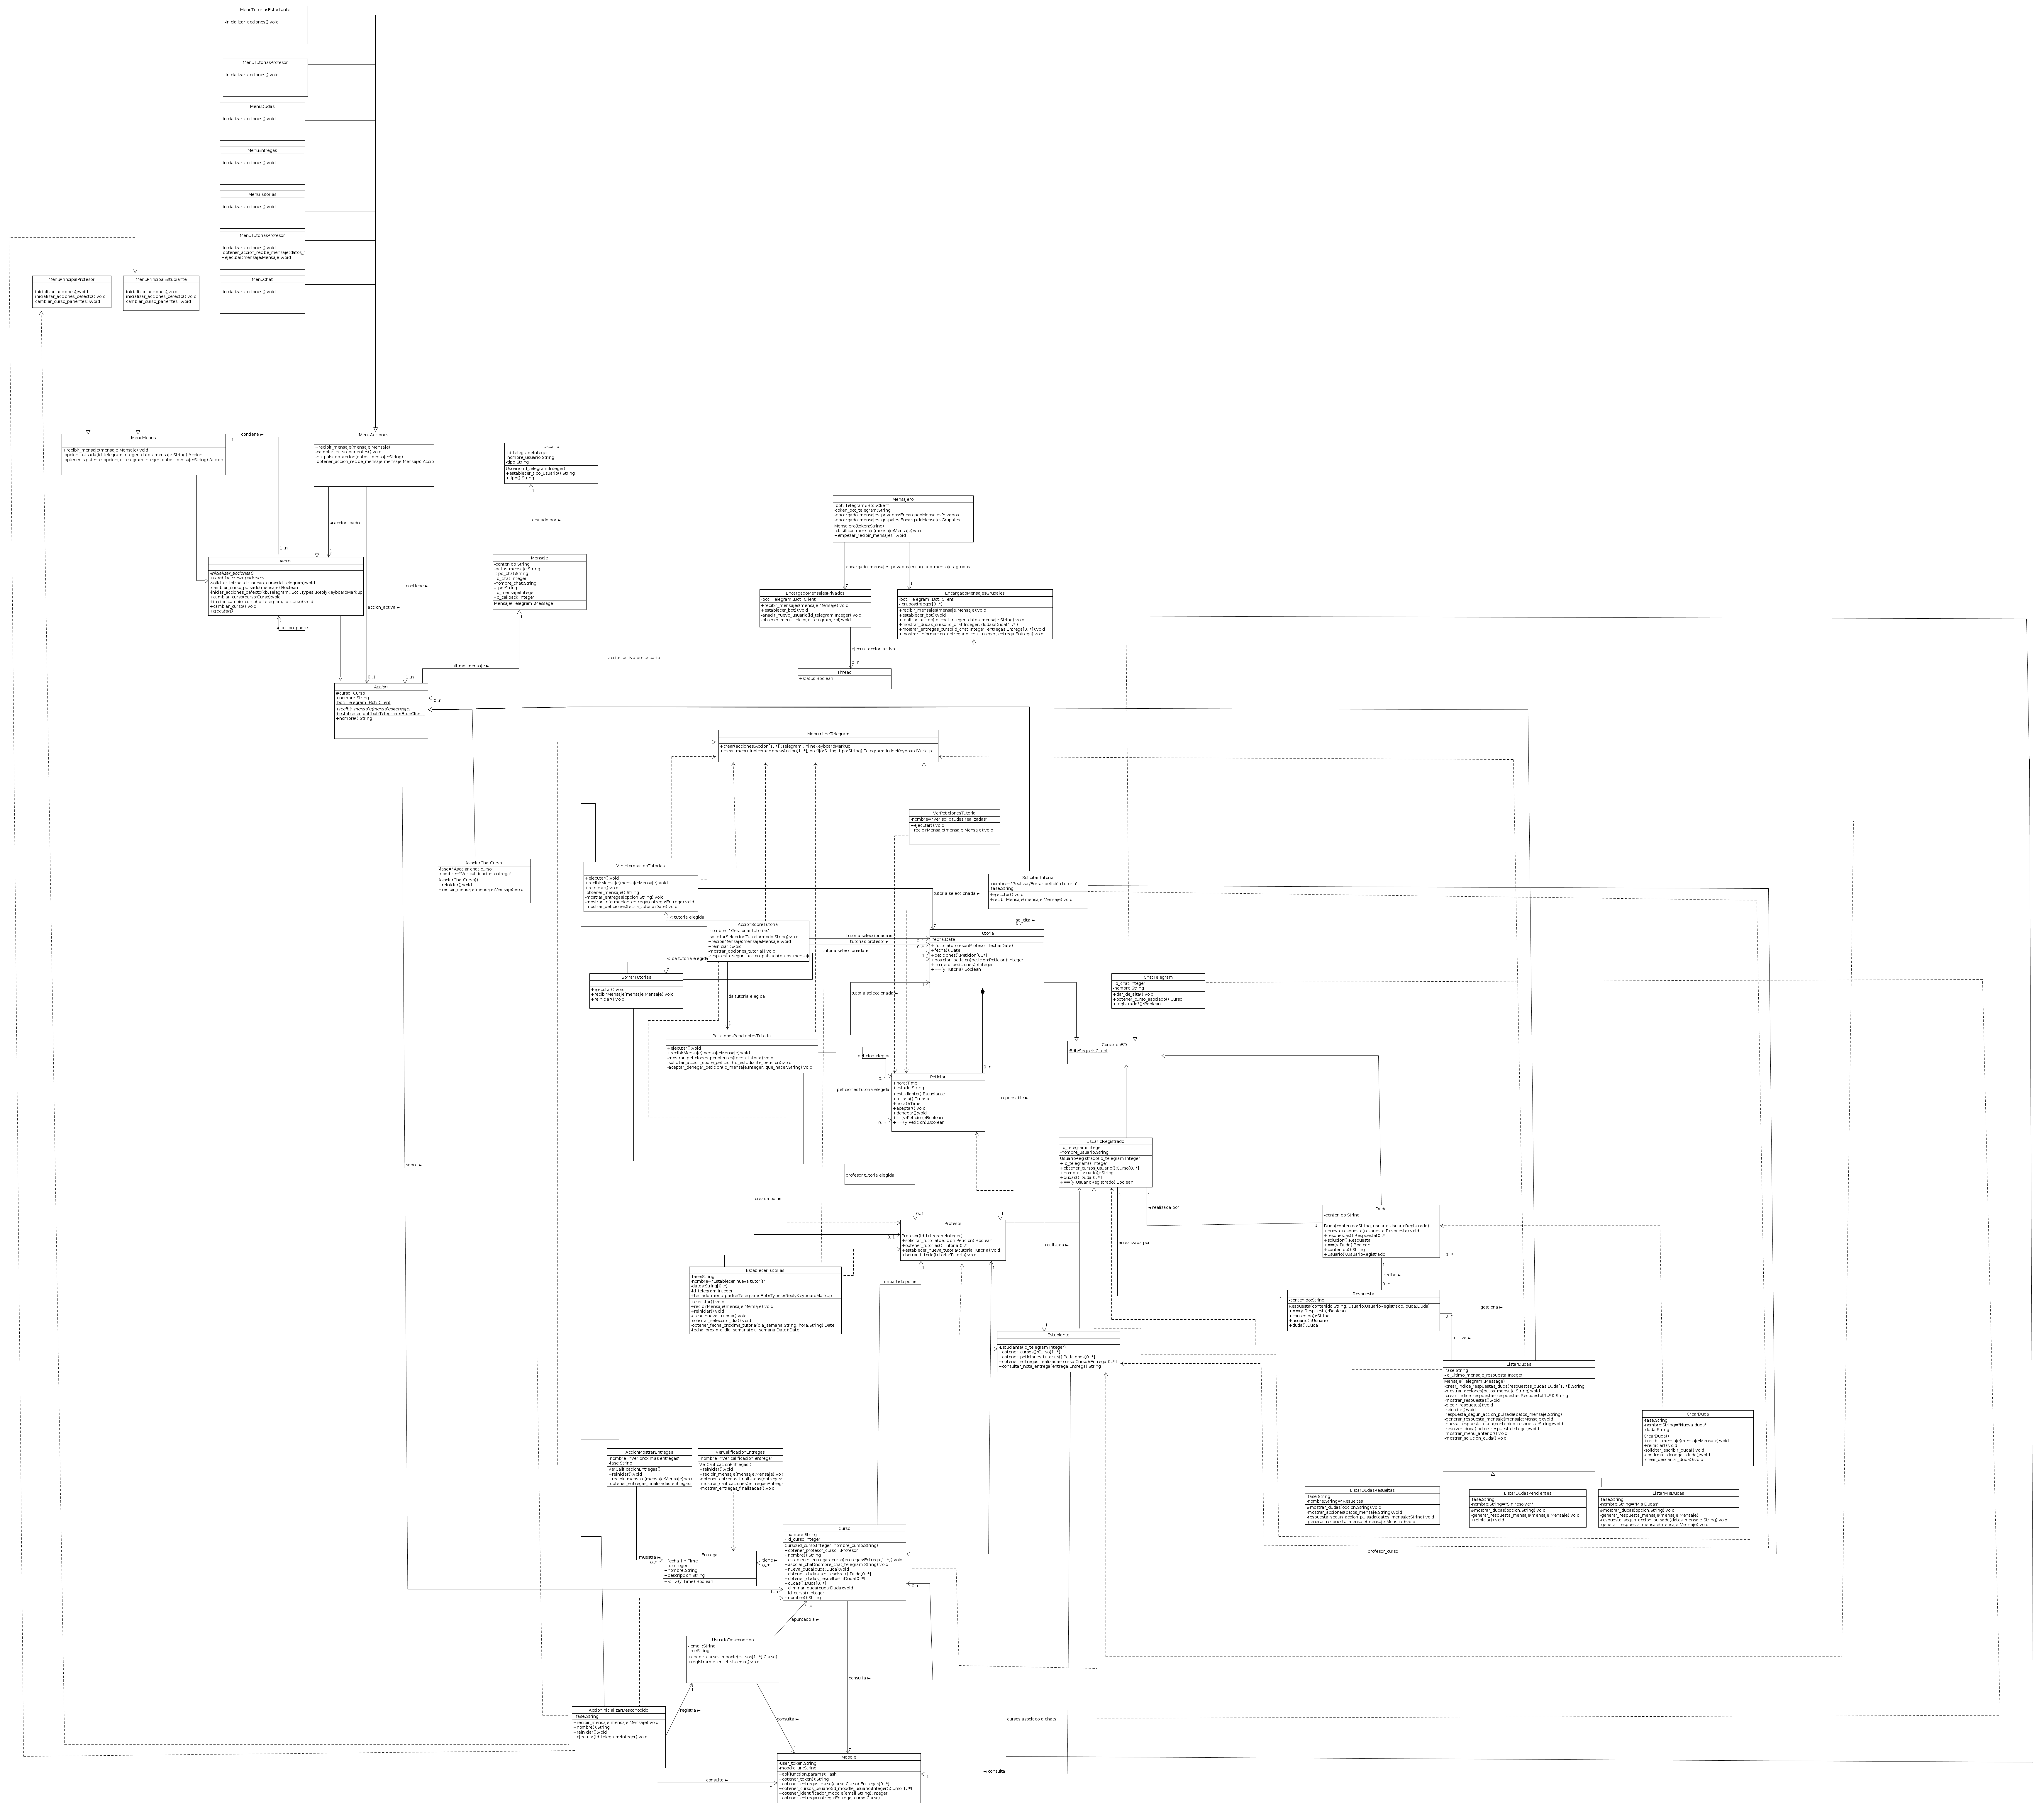
\includegraphics[width=1\textwidth, right]{imagenes/diagramas/diagrama_clases.png}  %el parámetro scale permite agrandar o achicar la imagen. En el nombre de archivo puede especificar directorios
\caption{Diagrama de clases del sistema}\label{figura10101}
\end{figure}
\subsection{Diseño de la configuración de Moodle}

Moodle, como bien se mecionaba en la introducción, proporciona una API accesible a través de lo que ellos llaman \textit{web services}  que permiten especificar las funciones que se pueden llamar de la API y por parte de qué usuarios en qué contexto. A los usuarios se le asigna un rol que es al que se le autoriza a usar un protocolo para comunicarse con los \textit{web services}, siendo también necesario autorizar individualmente a cada usario a que usen un \textit{web service}.  Los protocolos soportados son SOAP, REST o XML-RPC, nosotros vamos a utilizar REST por ser el más sencillo de manejar.
\par

Para el diseño de la configuración de Moodle hay que tener en cuenta lo que necesita el \textit{bot} de Moodle:
\begin{enumerate} 
\item \textit{Bot} necesita que Moodle verifique que los datos que introduce el usuario al registrarse son correctos.
\item \textit{Bot} necesita saber si el usuario que se da de alta es un profesor o un estudiante para darle acceso a una parte u otra de acciones.
\item Tiene que conocer los cursos en los que está matriculado un profesor para que cuando éste se dé de alta, poder registrar estos cursos como usables en el \textit{bot} y, al menos, también tiene que poder saber a qué cursos registrados en el \textit{bot} tiene acceso un estudiante en Moodle.
\item Necesita tener acceso a las entregas abiertas para los cursos que tiene registrados así como a datos como su fecha y si un estudiante lo solicita, a la nota de este estudiante.

\end{enumerate}

Para conseguir configurar Moodle de forma que el \textit{bot} pueda realizar los puntos descritos arriba y que el uso del mismo implique los menos privilegios posibles para evitar cualquier problema con la seguridad y el funcionamiento de la instancia de Moodle, he optado por un enfoque en el cual se empieza con ningún permiso e ir dando poco a poco hasta llegar a lo mínimo necesario.
\par
Los pasos que he seguido son los siguientes:
\begin{enumerate}
\item \textbf{Habilitar los webservices}, para lo cual hay que irse al apartado de \enquote*{Plugins} dentro de \enquote*{Site Administration} buscar \enquote*{Web services} y darle a habilitar.

\item \textbf{Habilitar el protocolo a utilizar}: dentro de Web services buscamos \enquote{Manage protocols} y habilitamos REST.
\begin{figure}[H] %con el [H] le obligamos a situar aquí la figura
\centering
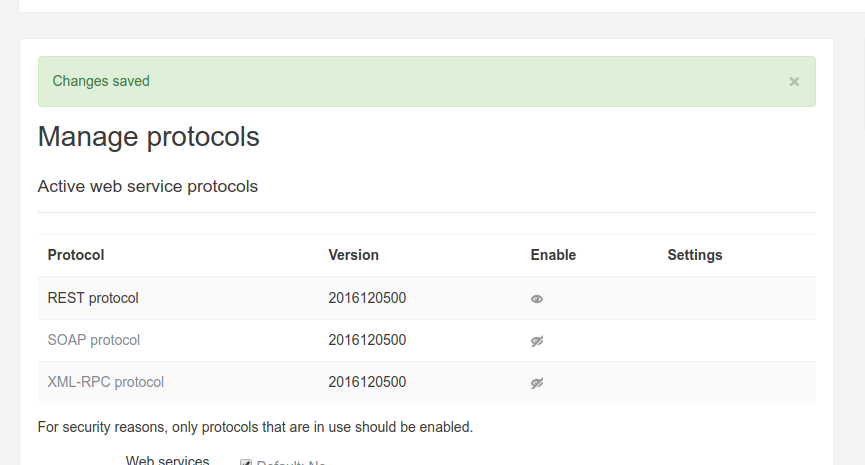
\includegraphics[scale=0.5]{imagenes/moodle/Screenshot_2017-08-25_10-28-32.png}  %el parámetro scale permite agrandar o achicar la imagen. En el nombre de archivo puede especificar directorios

\caption{Habilitando protocolo REST en Moodle}\label{figura410}
\end{figure}
\item Crear tres roles con contexto de sistema con los siguientes permisos mínimos:


\begin{tabular}{|p{5cm}|p{8cm}|}
\hline
\textbf{Nombre rol}
\newline

 &
 
\textbf{Permisos}
  \\
webservices\_bot
\newline

 &
 
\begin{itemize}
\item moodle/course:viewparticipants
\item moodle/user:viewdetails
\item moodle/user:viewhiddendetails
\item moodle/course:useremail
\item moodle/user:update

\end{itemize}
  \\
webservices\_estudiante
\newline

 &
 
\begin{itemize}
\item mod/assign:view
\end{itemize}
  \\
webservice\_profesor
\newline

 &
 

  \\
  \hline
\end{tabular}


\begin{figure}[H] %con el [H] le obligamos a situar aquí la figura
\centering
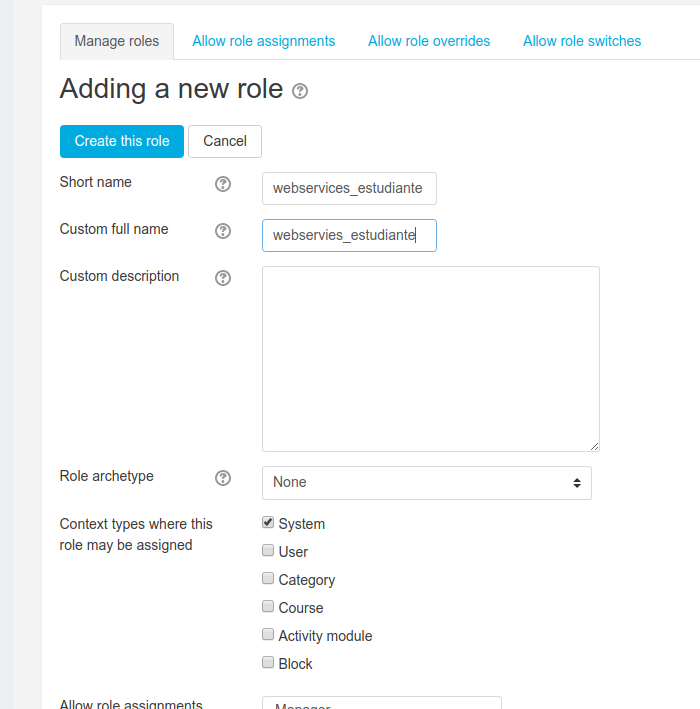
\includegraphics[scale=0.4]{imagenes/moodle/Screenshot_2017-08-25_11-11-23.png}  %el parámetro scale permite agrandar o achicar la imagen. En el nombre de archivo puede especificar directorios

\caption{Creando rol webservices\_student}\label{figura412}
\end{figure}

Estos permisos son los imprescindibles para poder utilizar las funciones descritas en la siguiente tabla. Si no fueran roles con contexto de sistema entonces no tendrían acceso a los \textit{web servies}.

\item Crear los siguientes webservices marcando \enquote*{enable} y \enquote*{Authorized users only}   con las siguientes funciones cada uno:

\begin{tabular}{|p{5cm}|p{8cm}|}
\hline
\textbf{Webservice}
\newline

 &
 
\textbf{Funciones}
  \\
webservices\_bot
\newline

 &
 
\begin{itemize}
\item \textbf{core\_enrol\_get\_users\_courses}: Permite al bot obtener los cursos de un usuario cuando éste se identifica ante el bot por primera vez.
\item \textbf{core\_user\_get\_users\_by\_field}: Permite obtener el identificador de moodle del usuario recién registrado, necesario para conocer las notas de su entrega.
\item \textbf{mod\_assign\_get\_assignments}: Permite al bot obtener las entregas abiertas para un curso junto con detalles como su fecha.
\end{itemize}
  \\
webservices\_estudiante
\newline

 &
 
\begin{itemize}
\item \textbf{mod\_assign\_get\_assignments}: Permite al estudiante ver las entregas para los cursos a los cuales tiene acceso.
\item \textbf{mod\_assign\_get\_submission\_status}: Un estudiante puede con su token, id de moodle e id entrega puede ver que calificación tiene en la entrega.
\end{itemize}
  \\
webservice\_profesor
\newline

 &
 

  \\
  \hline
\end{tabular}

\begin{figure}[H] %con el [H] le obligamos a situar aquí la figura
\centering
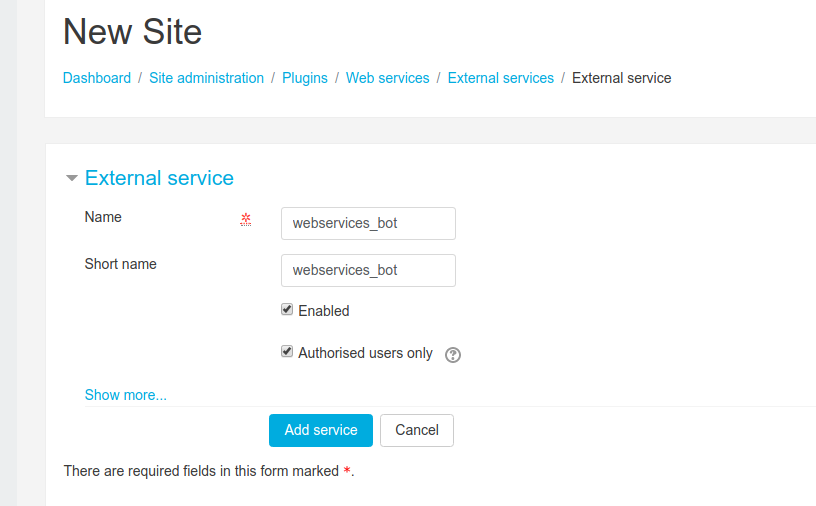
\includegraphics[scale=0.5]{imagenes/moodle/Screenshot_2017-08-25_11-24-11.png}  %el parámetro scale permite agrandar o achicar la imagen. En el nombre de archivo puede especificar directorios

\caption{Creando webservice llamado webservices\_bot}\label{figura415}
\end{figure}

\begin{figure}[H] %con el [H] le obligamos a situar aquí la figura
\centering
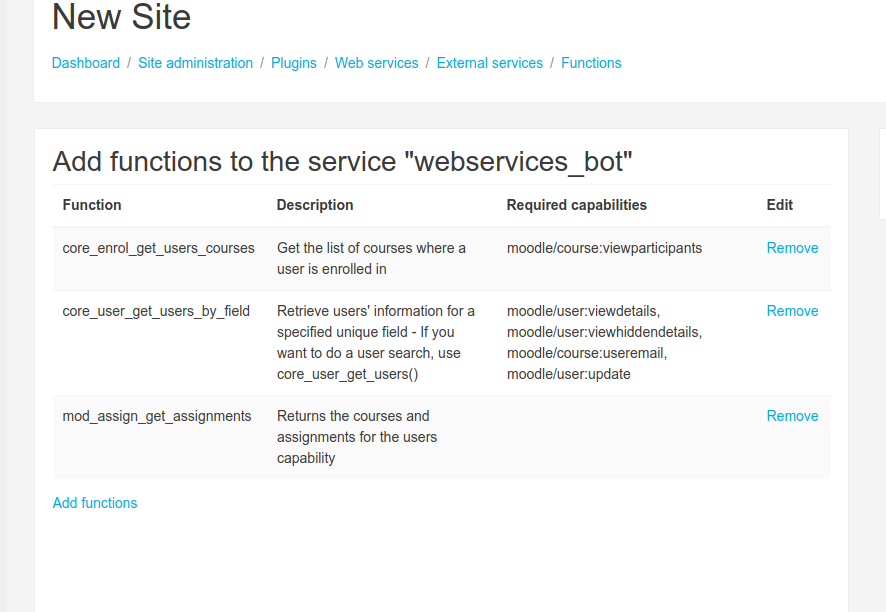
\includegraphics[scale=0.3]{imagenes/moodle/Screenshot_2017-08-25_11-27-44.png}  %el parámetro scale permite agrandar o achicar la imagen. En el nombre de archivo puede especificar directorios

\caption{Añadiendo funciones a el webservice llamado webservices\_bot }\label{figura415}
\end{figure}



\item Crear un usuario en Moodle para el bot.
\item Asignar el rol de webservices\_estudiante a los usuarios de moodle que quieren utilizar el bot como estudiantes, el webservices\_profesor a los profesores y el webservice\_bot al usuario que se ha creado para el bot. Como son roles de sistema es necesario irse al apartado \texttt{Site Administration > Users > Assign system roles services}:

\begin{figure}[H] %con el [H] le obligamos a situar aquí la figura
\centering
\includegraphics[scale=0.3]{imagenes/moodle/Screenshot_2017-08-25_14-40-20.png}  %el parámetro scale permite agrandar o achicar la imagen. En el nombre de archivo puede especificar directorios

\caption{Asignado el rol webservices\_bot al usuario creado en Moodle para el bot }\label{figura418}
\end{figure}

\item Añadir a los usuarios a los que se les ha asignado como rol webservices\_estudiante como usuarios autorizados a usar el recien creado webservices\_estudiante, a los que tienen rol webservices\_profesor añadir como usuarios autorizados al webservice webservices\_profesor y al usuario del bot con rol webservices\_bot añadirlo como usuario autorizado webservice\_bot. 

\begin{figure}[H] %con el [H] le obligamos a situar aquí la figura
\centering
\includegraphics[scale=0.3]{imagenes/moodle/Screenshot_2017-08-25_11-48-23}  %el parámetro scale permite agrandar o achicar la imagen. En el nombre de archivo puede especificar directorios

\caption{Asignado el rol webservices\_bot al usuario creado en Moodle para el bot }\label{figura419}
\end{figure}

\item Crear token para el usuario que se ha creado en Moodle para el bot. Esto se puede hacer bajo el apartado Web services buscando \texttt{Manage tokens}.



\begin{figure}[H] %con el [H] le obligamos a situar aquí la figura
\centering
\includegraphics[scale=0.3]{imagenes/moodle/Screenshot_2017-08-25_11-59-03.png}  %el parámetro scale permite agrandar o achicar la imagen. En el nombre de archivo puede especificar directorios

\caption{Creando token para el usuario en Moodle del bot }\label{figura419}
\end{figure}
\item Añadir en Moodle al usuario creado para el bot a cada curso que se quiera que tenga acceso el bot.

\begin{figure}[H] %con el [H] le obligamos a situar aquí la figura
\centering
\includegraphics[scale=0.3]{imagenes/moodle/Screenshot_2017-08-25_12-19-29.png}  %el parámetro scale permite agrandar o achicar la imagen. En el nombre de archivo puede especificar directorios

\caption{Añadiendo al usuario bot al curso curso7 }\label{figura420}
\end{figure}
\end{enumerate}



Una vez hecho esto podemos comprobar si tenemos acceso a las funciones de los \textit{web services} a traves de REST utilizando un navegador web:
\begin{figure}[H] %con el [H] le obligamos a situar aquí la figura
\centering
\includegraphics[scale=0.35]{imagenes/moodle/Screenshot_2017-08-25_12-32-18.png}  %el parámetro scale permite agrandar o achicar la imagen. En el nombre de archivo puede especificar directorios

\caption{Llamando a algunas de las funciones de webservices\_bot a través del navegador web }\label{figura420}
\end{figure}

Todo el proceso anteriomente descrito se puede encontrar en la sección \texttt{ Site Administration > Plugins > Web services} de cualquier instancia de Moodle.

\subsubsection{Justificación}

Se han creado tres \textit{web services} con tres roles diferentes ya que hay tres tipos de usuarios y cada uno necesita acceder a un conjunto de funciones diferentes. Si tuvieramos un solo rol y un solo \textit{web service} entonces algunos usuarios tendrían más permisos de los necesarios y acceso a funciones de la API que no les hacen falta.
\par
Ejemplo: al \textit{bot} no le hace falta hacer llamadas a la función que obtiene calificaciones de la entrega y por tanto mejor no darle acceso. 
\par
Cada usuario del sistema en el momento que introduce sus datos de Moodle para empezar a usar el bot éste obtiene una token de usuario y con esa token el usuario solamente tiene acceso a su información individual (caso de los estudiante que cuando llaman a \texttt{mod\_assign\_get\_submission\_status} les devuelve datos de las entregas del usuario cuya token se utiliza para llamar al \textit{web service}.)
\par
Hace falta un token aparte para el \textit{bot} porque éste necesita conocer información común de un curso como las entregas que hay abiertas, si no tiene token entonces no hay acceso. Además si no creáramos un usuario aparte para el \textit{bot} entonces no se puede controlar a qué cursos tienen acceso los usuarios del \textit{bot}. Obligando a añadir al bot a un curso de Moodle hacemos que los usuarios que soliciten al bot usarlo sólamente tengan acceso a aquellos cursos en los que el bot ha sido añadido. Esto es importante ya que dando rol con contexto de sistema a un usuario hacemos que tenga acceso con su token a todos los cursos en los que están matriculados en Moodle (limitado a las funciones permitidas en su webservice y a los permisos de su rol) tanto si el profesor responsable de ese curso quiere o no quiere utilizar los webservices de Moodle para ese curso.

\newpage
\subsection{Diseño de la base de datos}

La estructura lógica de la base de datos se puede observar en el siguiente diagrama ER:

\begin{figure}[H] %con el [H] le obligamos a situar aquí la figura
\centering
\includegraphics[scale=0.2]{imagenes/diagramas/base_datos/ER.png}  %el parámetro scale permite agrandar o achicar la imagen. En el nombre de archivo puede especificar directorios

\caption{Diagrama ER de la base de datos }\label{figura520}
\end{figure}
Se pueden apreciar las necesidades de almacenamiento que va a tener nuestra aplicación y podemos extraer el esqueleto de la base de datos con sus relaciones, claves externas, primarias... \par
Tras realizar el paso a tablas de este diagrama y efectuar el paso a la tercera forma normal obtenemos el siguiente esquema de la base de datos:


 \begin{figure}[H] %con el [H] le obligamos a situar aquí la figura
\includegraphics[width=1.2\textwidth, right]{imagenes/diagramas/base_datos/esquema_tablas_normalizadafn3.png}  %el parámetro scale permite agrandar o achicar la imagen. En el nombre de archivo puede especificar directorios
\caption{Esquema base datos en tercera forma normal}\label{figura5211}
\end{figure}



\subsection{Diseño de los tests}

En el desarrollo de la aplicación se está siguiendo la programación orientada a objetos como paradigma de programación. Para verificar el correcto funcionamiento de las clases que la componen se hace uso de test unitarios que prueban la \enquote*{interfaz} o parte pública de la clase proporcionándole datos de prueba y comprobando si los resultados devueltos por ésta son los esperados.
\par
A la hora de diseñar estos tests unitarios hay que tener en cuenta que básicamente hay dos tipos de clases: aquellas que reciben un mensaje y realizan algo con este (bien sea extraer los datos de éste y realizar una acción o entregar el mensaje a la clase responsable) y las que acceden a la base de datos y Moodle. Para los tests de las primeras se hará uso de stubs para simular clases con una serie de métodos predefinidos que devuelven datos ideales y  de mocks para monitorizar si la clase bajo prueba realiza las acciones deseadas cuando se le entrega un mensaje con unas características predeterminadas.\\
Para las segundas debido a la dificultad de simular una base de datos se optará por crear una base de datos \enquote*{desechable} en la cual se introducen una serie de datos prefijados y se prueba el comportamiento de la interfaz pública de estas clases, bien llamando a sus métodos públicos y comprobando el resultado devuelto, o bien comprobando el efecto sobre la base de datos.

%
\chapter{}

\section{Implementación}

\subsection{Programa}
A la hora de implementar el programa una variable importante es la facilidad con la que se puede trabajar con la API para bots de Telegram. Debido a ello, y como quería que el proyecto fuera el desarrollo de pradobot y no de un programa para trabajar con la API de Telegram, opté por el uso de una librería que facilitara la tarea. En el momento de empezar la implementación las más populares eran:


\begin{itemize}
\item Para NodeJS: \url{https://github.com/yagop/node-telegram-bot-api}
\item Para Python: \url{https://github.com/python-telegram-bot/python-telegram-bot}
\item Para Golang: \url{https://github.com/go-telegram-bot-api/telegram-bot-api}
\item Java: \url{https://github.com/rubenlagus/TelegramBots}
\item Ruby: \url{https://github.com/atipugin/telegram-bot-ruby}
\end{itemize}

Teniendo conocimiento de Ruby y habiendo probado en alguna asignatura el correcto funcionamiento de la librería de Ruby, decidí usarla. Esta librería te permite hacer uso de los métodos de la API para bots de Telegram con un formato \textit{camel\_case} es decir las palábras de los métodos en minúscula y separadas por una barra baja. Por lo demás acepta los mismos parámetros:



\begin{figure}[H] %con el [H] le obligamos a situar aquí la figura
\centering
\includegraphics[scale=0.42]{imagenes/random/Screenshot_2017-08-27_08-16-42.png}  %el parámetro scale permite agrandar o achicar la imagen. En el nombre de archivo puede especificar directorios

\caption{Uso del método SendMessage por parte del bot }\label{figura531}
\end{figure}
El único inconveniente que tiene es que solamente puede haber una instancia del cliente que recibe mensajes. Esto es debido a que para que un bot de Telegram reciba los mensajes que le llegan tiene dos alternativas \textit{long polling} y \textit{Webhook}\cite{telegram10}\cite{telegram20} :
\begin{itemize}
\item \textit{Long polling}: El bot periódicamente llama a los servidores de Telegram utilizando un método que devuelve los 100 primeros mensajes  sin contestar que tiene el bot. Más lento pero mucho más facil de utilizar.
\item \textit{Webhook}: Hace falta implementar un servidor con una IP pública o un nombre de dominio e indicarle a Telegram que cuando se le manda un mensaje al bot éste lo redirija a este servidor. Rápido pero más complicado de montar.
\end{itemize}

El bot ha sido implementado haciendo uso de long polling y la implementación que realiza la librería utilizada  solamente deja que haya una instancia del bot \textbf{escuchando}:


\begin{figure}[H] %con el [H] le obligamos a situar aquí la figura
\centering
\includegraphics[scale=0.7]{imagenes/random/Screenshot_2017-08-27_11-49-39.png}  %el parámetro scale permite agrandar o achicar la imagen. En el nombre de archivo puede especificar directorios

\caption{ }\label{figura531}
\end{figure}

Lo cual a efectos prácticos implica que solamente puede haber un único :

\begin{lstlisting}

      botox.listen do |message|
        begin
          .....
        end
      end
 
\end{lstlisting}



\par 

 Una vez tienes el programa escrito en ruby que es capaz de obtener los mensajes que se le envían al bot por Telegram y de interactuar con los usuarios quedan dos partes más: la base de datos y la instancia de Moodle. 
 
 \subsubsection{Git-Github}
 
  Con la intención de que la construcción de la aplicación fuera lo más transparente posible y de dar la posibilidad de que otras personas pudieran contribuir a ella, se ha he hecho uso de la plataforma de desarrollo colaborativo Github y del sistema de control de versiones Git durante todo el proceso de implementación de la aplicación. 
  
  Github permite, entre otras cosas, ver los cambios realizados en el código desde el primer momento, la creación de \textit{issues} que pueden ser utilizados para indicar algún fallo en la aplicación y junto con git permite tener varias versiones del código.
  
 Todo el código del programa se puede encontrar en \url{https://github.com/LuisGi93/pradobot}.


\subsection{Base de datos}

Como base de datos he utilizado PostgreSQL principalmente porque es \textit{opensource}, fácil de instalar y no he visto en ningún sitio que tenga diferencias de rendimiento significativas comparada con otras bases de datos importantes. Aún así debido al uso de una librería de ruby llamada \href{https://github.com/jeremyevans/sequel}{Sequel}, que hace de adaptador entre la aplicación y la base de datos, se podría utilizar cualquier otra base de datos.

Sequel hace uso de ORM para la comunicación con la base de datos. También ofrece una capa de  abstracción entre aplicación y el manejo de todo lo relacionado con la interacción sobre la base de datos. Algunas de las carácteristicas relevantes para su uso:

\begin{itemize}
\item Ofrece configurar el número de conexiones disponibles para acceder a la base de datos.\cite{sequel1}
\item Una instancia de la \enquote*{conexión} con la base de datos hace uso de manera transparente para el programador de múltiples hebras para utilizar las conexiones disponibles de la base de datos. Lo cual implica que una misma variable  puede ser usada a lo largo del programa para realizar consultas con la base de dato sin que una consulta paralice al programa ya que serán ejecutadas por diferentes hebras.
\item Las conexiones descritas en el primer punto se levantan en el momento en que se lanza la primera consulta \cite{sequel2} quedando latentes a la espera de ser usadas por las siguientes consultas. Es decir no se abre una sesión con la base de datos, se realiza la consulta y se cierra la conexión, sino que está diseñado para que una misma conexión sea usada por diferentes consultas. Una correcta configuración del número de conexiones que se quiere que se tengan disponibles para la base de datos y del número de hebras a usar sobre esas conexiones es importante para un uso óptimo de la base de datos. Pradobot es un prototipo, y si se quisiera utilizar en un ambiente \enquote*{real}, esta sería una de las cosas que habría que mirar con lupa.
\item La abstracción que te ofrece el uso de ORM simplifica mucho el trabajar con la base de datos.
\end{itemize}

\subsection{Moodle}

Durante el desarrollo del programa se ha utilizado la versión 3.2.1 de Moodle. Aunque también se ha probado con la versión 3.0.10 y sea posiblemente la versión mínima soportada por el programa ya que las anteriores versiones no tienen algunas de las funciones de la API de Moodle utilizadas por el programa.


\subsection{Despliegue}

Para facilitar la instalación de la aplicación incluimos un fichero \enquote*{Vagrantfile} que permite la creación de una máquina virtual con Ubuntu 14.04 en Amazon AWS con pradobot y todas sus dependencias instaladas en ella. El contenido del Vagrantfile es el siguiente:

Para poder utilizar el Vagrantfile necesitamos tres programas: 

\begin{enumerate}
\item Instalar programa vagrant para nuestra distribución.
\item aws-cli: programa que nos permite conectarnos con nuestra cuenta en amazon aws y que genera credenciales para Vagrantfile (pip install awscli) .
\item Plugin aws para vagrant (vagrant plugin install vagrant-aws)
\end{enumerate}

El contenido de un Vagrantfile es similar al siguiente:
\begin{lstlisting}

Vagrant.configure("2") do |config|
  config.vm.box = "dummy"

  config.vm.define "pradobot-aws" do |host|
    host.vm.hostname = "pradobot-aws"
  end
  config.vm.provider :aws do |aws, override|
    aws.access_key_id = "xxx"
    aws.secret_access_key = "xxx"
    aws.session_token = "xxx"
    aws.keypair_name = "pradobotllave"
    aws.region= "us-west-2"
    aws.security_groups = "migruposeguro"
    aws.instance_type= 't2.micro'
   
    aws.ami = "ami-d57dcfb5"

    override.ssh.username = "ubuntu"
    override.ssh.private_key_path = "pradobotllave.pem"
  end
  
    config.vm.provision :ansible do |ansible|
	ansible.playbook = "pradobot.yml"
	ansible.force_remote_user= true
  end
end
 
\end{lstlisting}

El Vagrantfile cuenta con los siguientes elementos:
\begin{itemize}
\item \textbf{aws.secret\_access\_key}, \textbf{aws.session\_token}: Claves efímeras que nos autorizan para crear máquinas virtuales en nuestra cuenta durante 48 horas. Generadas utilizando aws-cli:

\begin{figure}[H] %con el [H] le obligamos a situar aquí la figura
\centering
\includegraphics[scale=0.6]{imagenes/random/1234sts.png}  %el parámetro scale permite agrandar o achicar la imagen. En el nombre de archivo puede especificar directorios

\caption{Utilizando aws-cli para generar claves efímeras para el despliegue}\label{figura90}

\end{figure}
\item \textbf{aws.keypair\_name}: Generada utilizando:
\begin{lstlisting}
 aws ec2 create-key-pair --key-name pradobotllave --query 'KeyMaterial' --output text > pradobotllave.pem
\end{lstlisting}
\item \textbf{aws.security\_groups}: Grupo de seguridad en Amazon AWS en  podemos especificar que puertos de entrada/salida están habilitados en la máquina virtual y que IPs aceptamos.
\item \textbf{aws.region},\textbf{aws-instance\_type},\textbf{aws.ami}: Especifican la región, las características del servidor donde se ejecuta la máquina virtual y el sistema operativo.
\item Por último \textbf{config.vm.provision} especifica que queremos usar Ansible para aprovisionar la máquina virtual:
\begin{itemize}
\item \textbf{ansible.playbook}: script que utilizará ansible para aprovisonar la máquina virtual.
\end{itemize}
\end{itemize}

\subsection{Aprivisionamiento}

El aprovisionamiento de la máquina virtual creada por vagrant se hace utilizando el programa Ansible. Ansible hace uso de ssh y de un tipo de archivos llamados \enquote*{playbooks} en las cuales se especifican las órdenes necesarias para el aprovisonamiento de la máquina virtual. El playbook utilizado por pradobot es el siguiente:
\begin{lstlisting}

---
---
- hosts: all
  user: ubuntu
  sudo: yes    
  roles:
    - { role: rvm_io.ruby,
        tags: ruby,
        rvm1_rubies: ['ruby-2.3.1'],
        rvm1_user: 'ubuntu',
        become: true
      }
      
  tasks:       


#Por alguna razon instala todos los paquetes menos libpq-dev

  -  name: Instalamos  paquetes necesarios
     become: true
     action: >
      {{ ansible_pkg_mgr }} name= {{ item }}  state=installed update_cache=yes
     with_items:
      - build-essential
      - ruby-dev
      - libpq-dev
      - ruby
      - git
      - libgdbm-dev
      - libncurses5-dev
      - automake
      - libtool
      - bison
      - libffi-dev
     
  -  name: instalamos git
     apt:
       name: git
       state: present

  -  name: instalamos libpq-dev
     apt:
       name: libpq-dev
       state: present

  -  name: clonamos repo de la web
     become: true  
     become_user: ubuntu
     shell: git clone  https://github.com/LuisGi93/pradobot.git
     args:
       creates: pradobot
       executable: /bin/bash

  -  name: Instalamos el proyecto
     become: true  
     become_user: ubuntu 
     shell: source ~/.rvm/scripts/rvm && bundle install 
     args:
       chdir: pradobot
       executable: /bin/bash
     
      -  name: Creamos las tablas de la base de datos
     become: true  
     become_user: ubuntu 
     shell: source ~/.rvm/scripts/rvm && export URL_DATABASE_TRAVIS="" &&  ruby config/primer_inicio_aplicacion.rb
     args:
       chdir: pradobot
       executable: /bin/bash
\end{lstlisting}

En el cual podemos distinguir las siguientes partes relevantes:
\begin{itemize}

\item \textbf{hosts}, \textbf{user}: Indicamos el nombre de la máquina a la que se va a conectar Ansible utilizando ssh.
\item \textbf{user}: nombre del usuario con el cual se inicia sesión en dicha máquina utilizan ssh.
\item \textbf{sudo}: Indicamos si se va utilizar sudo o no.
\item \textbf{roles}:  Indicamos que para ejecutarse este playbook se necesitan una serie de archivos, en este caso rvm que explico más abajo para que sirve.
\item \textbf{tasks}: Tareas a ejecutar por Ansible secuencialmente, algunos de los elementos que pueden tener son:
\begin{itemize}
\item \textbf{name}: nombre descriptivo.
\item \textbf{become}: implica el uso de sudo.
\item \textbf{become\_user}: implica el usuario a utilizar.
\item \textbf{shell}: el comando se tiene que ejecutar en una shell.
\item \textbf{apt}: requiere el uso del administrador de paquetes.
\end{itemize}

\end{itemize}

El script en primer lugar instala los paquetes necesarios, tras lo cual clona el proyecto desde github creando el directorio pradobot y procede a instalar las dependencias de pradobot utilizando RVM y Bundler.\\
RVM es un programa que permite la ejecución de otro programa escrito en ruby en el entorno de ruby deseado, en mi caso pradobot necesita la versión 2.3.1 de ruby que no se encuentra en los repositorios de Ubuntu. Bundler automatiza la instalación de las librerías que necesita una aplicación de ruby para lo cual hace uso de un archivo llamado Gemfile:
\begin{lstlisting}[language=Ruby]

source "https://rubygems.org"
gem 'sequel'
gem 'pg'
gem 'rake'
gem 'rspec'
gem 'telegram-bot-ruby'
gem 'json'
gem 'rufus-scheduler'
gem 'activesupport'
gem 'daemons'
gem 'typhoeus'
group :test do
  gem 'rake'
end
\end{lstlisting}
En el se especifican las librerías a obtener, su versión si se quiere y de donde obtenerlas. Por último inicia la ejecución de pradobot.

\subsection{Control ejecución}

Una vez hemos creado la máquina con Vagrant y haberla aprovisionado utilizando Ansible, tenemos que poder controlar el inicio y fin de ejecución de la aplicación de manera automática. Para ello vamos a utilizar una herramienta llamada Capistrano. Capistrano permite la ejecución de comandos remotos a través de ssh. En primer lugar lo instalamos haciendo \texttt{gem install capistrano} tras lo cual ejecutamos la orden \texttt{cap install} en el directorio de nuestro proyecto. Esto provocará la generación de una serie de archivos. Buscamos \enquote*{config/deploy.rb} y le añadimos información para la autenticación via ssh:
\begin{lstlisting}[language=Ruby]

set :ssh_options, {
  forward_agent: true,
  auth_methods: ["publickey"],
  keys: ["path_a_llave_pem/pradobotllave.pem"]
}

\end{lstlisting}

En Capistrano se definen "tareas" donde defines que es lo que quieres que haga capistrano. Para establecer la tarea creamos un fichero en lib/capistrano/tasks acabado en .rake y en el defino la siguiente tarea:


\begin{lstlisting}[language=Ruby]

require "resolv-replace.rb"

role :yoquese, "yoquese"


namespace :pradobot do
  desc "Iniciamos la aplicacion"

  task :daemon_start do
	on "ubuntu@ip.us-west-2.compute.amazonaws.com" do
		execute  'source ~/.rvm/scripts/rvm && export TOKEN_BOT_MOODLE="" && export MOODLE_HOST="" && export TOKEN_BOT="" && export URL_DATABASE_TRAVIS="" && nohup ruby pradobot/bin/run.rb && true & '
	end
  end
  
  desc "Paramos la aplicacion"  
  task :daemon_stop do
	on "ubuntu@ip.us-west-2.compute.amazonaws.com" do
		execute  'pkill ruby'
	end
  end
end

\end{lstlisting}

Con lo cual podemos ejecutar el comando \texttt{cap production pradobot:daemon\_start} para iniciar su ejecución y pararlo utilizando \texttt{cap production pradobot:daemon\_stop}. \par Para el inicio de la ejecución se hace uso del comando nohup, que desliga a un proceso de la terminal de tal forma que cuando se lanza el programa en segundo plano (\texttt{ruby pradobot/bin/run.rb \&\& true \&}) su ejecución no termina al finalizar la ejecución de la orden por ssh. 

\subsection{Tests}


Los tests se han implementado utilizando Rake. Rake es una herramienta que permite entre otras cosas ejecutar tests de ruby para lo cual necesita disponer de un archivo llamado Rakefile en el cual se le indica dónde puede encontrar los tests y qué pasos hay que dar para ejecutarlos. El Rakefile de pradobot es el siguiente:

\begin{lstlisting}[language=Ruby]

require 'rake/testtask'
require 'rspec/core/rake_task'
require_relative 'config/crear_tablas_bd'
require 'sequel'



namespace :tasks do
  namespace :db do
    namespace :test do

      desc "Creamos base de datos test"
      task :crear  do
        db=Sequel.connect(ENV['URL_DATABASE'])
        begin
          db.run "CREATE DATABASE bd_prueba"
        rescue Sequel::Error
          db.run "DROP DATABASE bd_prueba"
          db.run "CREATE DATABASE bd_prueba"
        end
        db.disconnect
        db=Sequel.connect(ENV['URL_DATABASE']+'/bd_prueba')
        crear_tablas(db)
        db.disconnect
        ENV['URL_DATABASE_ORIGINAL']=ENV['URL_DATABASE']
        ENV['URL_DATABASE']=ENV['URL_DATABASE_PRUEBA']
      end

      RSpec::Core::RakeTask.new(:tests_bd) do |t|
          t.pattern = Dir.glob('test/test_*.rb')

          t.rspec_opts = '--format documentation'
      end

      desc "Borramos la base de datos"
      task :destruir  do
        ENV['URL_DATABASE']=ENV['URL_DATABASE_ORIGINAL']
        db=Sequel.connect(ENV['URL_DATABASE'])
        db.run "DROP DATABASE bd_prueba"
        db.disconnect
      end

    end

  end




end


desc "Ejecutamos los test sobre la base de datos"
task :default => ['tasks:db:test:crear', 'tasks:db:test:tests_bd', 'tasks:db:test:destruir' ]
\end{lstlisting}

En él se especifican las tareas que tiene que ejecutar Rake:
\begin{itemize}
\item \textbf{task :default}: Es la tarea que se llama por defecto subdividida en tres tareas:
\begin{enumerate}
\item \textbf{tasks:db:test:crear} : Crea una base de datos de prueba e insertamos las tablas que componen la aplicación.
\item \textbf{tasks:db:test:tests\_bd} : Indica a Rake que ejecute como tests todos los archivos contenidos en la carpeta test/ y que empiecen por test\_.
\item \textbf{tasks:db:test:destruir}: Destruye la base de datos creada en el paso 1.
\end{enumerate}

\end{itemize}

Para la realización de los tests he hecho uso de la librería RSpec que proporciona las herramientas necesarias para la realización de los mocks y los stubs. Un ejemplo de test puede ser:

\begin{lstlisting}[language=Ruby]

describe CrearDuda do
  before(:each) do
    @stub_bot = double('bot')

    Accion.establecer_bot(@stub_bot)

    allow(@stub_mensaje).to receive_message_chain(:usuario, :id_telegram) { 66 }

    @stub_curso = double('curso')
    allow(@stub_curso).to receive(:nombre) { 'nombre del curso' }
    allow(@stub_curso).to receive(:id_moodle) { 5 }
    stub_padre = double('accion_padre')
    allow(stub_padre).to receive(:cambiar_curso)
    allow(stub_padre).to receive(:cambiar_curso_parientes)
    allow(stub_padre).to receive(:curso) { @stub_curso }
    @accion = MenuDudas.new(stub_padre)
    @accion.cambiar_curso(@stub_curso)
  end

  it 'Cuando recibe el primer mensaje muestra mensaje explicativo de que realiza' do
    allow(@stub_mensaje).to receive(:datos_mensaje) { 'Nueva duda' }
    expect(@stub_bot).to receive_message_chain(:api, :send_message) { |arg1|
      arg1.keys.should_not include(:reply_markup)
      arg1[:text].should eq("Escriba a continuaci\otilden la duda que desea crear relacionada con *nombre del curso*:\n")
    }
    @accion.recibir_mensaje(@stub_mensaje)
  end

  it 'Debe mandar mensaje que incluya el texto de la duda y el curso con opciones para confirmar la creaci\otilden de la duda' do
    allow(@stub_mensaje).to receive(:datos_mensaje) { 'Nueva duda' }

    allow(@stub_bot).to receive_messag_chain(:api, :send_message)
    @accion.recibir_mensaje(@stub_mensaje)

    allow(@stub_mensaje).to receive(:datos_mensaje) { 'Contenido nueva duda' }

    expect(@stub_bot).to receive_message_chain(:api, :send_message) { |arg1|
      arg1.keys.should include(:chat_id, :text, :reply_markup)
      arg1[:text].should include('nombre del curso')
      arg1[:text].should include('Contenido nueva duda')
      arg1[:reply_markup].should be_instance_of(Telegram::Bot::Types::InlineKeyboardMarkup)
    }
    @accion.recibir_mensaje(@stub_mensaje)
  end
  
   .....
end

\end{lstlisting}

Al principio se define stub\_bot que actúa a la vez como mock y stub para, a continuación, especificarse los métodos que tiene que aceptar mediante la orden \texttt{allow(stub).to receive(nombre método)[ datos respuesta ]}.
\par
En esta fragmento de código podemos encontrar dos tests que vienen compredidos entre el \texttt{it .. do} y el \texttt{end} que lo cierra. En los dos tests mostrados  se definen mediante la orden \texttt{expect(stub).to receive(nombre método)[  argumentos ]} las expectativas del test.
\begin{itemize}
 \item En el primero el objeto stub\_bot espera que se llame al método 
 \texttt{stub\_bot.api.send\_message} que se le pase como argumento un objetivo tipo hash que entre sus llaves no tenga una llamada \texttt{:reply\_markup} y sí una llave llamada \texttt{text} que tenga el valor de \texttt{"Escriba a continuación la duda que desea crear relacionada con *nombre del curso*:"}. 
 \item El segundo test es parecido solo que ahora se observa el comportamiento de la clase cuando ha recibido su segundo mensaje y se comprueba qué le manda al bot como respuesta de este segundo mensaje.
 \end{itemize}
 \par
 
 Por último para ver la cobertura sobre el código del programa que tienen nuestros tests y comprobar en qué puntos de la aplicación faltan pruebas unitarias por realizar se ha hecho de una librería llamada \textbf{SimpleCov}.

%
\chapter{}

\section{Pruebas}

\subsection{Prueba despliegue}

Para probar la creación de la máquina virtual en Amazon AWS vamos a mostrar el resultados de ejecutar el Vagrantfile mostrado anteriomente. Es necesario ejecutar la orden \texttt{vagrant up --provider=aws}:
\begin{figure}[H] %con el [H] le obligamos a situar aquí la figura
\centering
\includegraphics[scale=0.3]{imagenes/random/2017-09-05-172749_1366x768_scrot.png}  %el parámetro scale permite agrandar o achicar la imagen. En el nombre de archivo puede especificar directorios

\caption{Ejecutando los tests de la aplicación}\label{figura92}

\end{figure}

En la salida de la orden se pueden ver las características de la máquina virtual creada tras lo cual una vez está habilitado ssh se ejecuta el playbook de Ansible:

\begin{figure}[H] %con el [H] le obligamos a situar aquí la figura
\centering
\includegraphics[scale=0.3]{imagenes/random/2017-09-05-174148_1366x768_scrot.png}  %el parámetro scale permite agrandar o achicar la imagen. En el nombre de archivo puede especificar directorios

\caption{Finalización de aprovisonamiento con Ansible}\label{figura94}

\end{figure}

Por último ejecutamos Capistrano para iniciar y parar la aplicación:

\begin{figure}[H] %con el [H] le obligamos a situar aquí la figura
\centering
\includegraphics[scale=0.3]{imagenes/random/2017-09-05-184638_1366x768_scrot.png}  %el parámetro scale permite agrandar o achicar la imagen. En el nombre de archivo puede especificar directorios

\caption{Iniciamos la ejecución de la aplicación utilizando Capistrano}\label{figura905}

\end{figure}

\begin{figure}[H] %con el [H] le obligamos a situar aquí la figura
\centering
\includegraphics[scale=0.3]{imagenes/random/2017-09-05-184725_1366x768_scrot.png}  %el parámetro scale permite agrandar o achicar la imagen. En el nombre de archivo puede especificar directorios

\caption{Detenemos la ejecución de la aplicación}\label{figura910}

\end{figure}


Capistrano puede que al hacer el \texttt{cap production pradobot:daemon\_start} se quede paralizado siendo necesario hacer un control-C para que se salga de la terminal. La aplicación se seguirá ejecutando normalmente.


\subsection{Tests}

Para ejecutar los tests unitarios que componen la aplicación es necesario ejecutar la orden \texttt{rake} en el directorio en el cual se encuentra el Rakefile. Esto hará que rake lea los ficheros especificados en el Rakefile y ejecute los tests contenidos en ellos uno a uno:

\begin{figure}[H] %con el [H] le obligamos a situar aquí la figura
\centering
\includegraphics[scale=0.4]{imagenes/random/Screenshot_2017-09-04_18-28-17.png}  %el parámetro scale permite agrandar o achicar la imagen. En el nombre de archivo puede especificar directorios

\caption{Tras ejecutar los tests de la aplicación}\label{figura92}

\end{figure}

Como podemos ver en la imagen superior se muestra en verde cada test que ha pasado satisfactoriamente dando al final un resumen del número de tests ejecutados (156 examples) y de cuántos han fallado (0 failures) indicando además cuánto tiempo se han tardado en ejecutar los tests. También se muestra el porcentaje de código que cubren nuestros tests (93.13\%) generandose un reporte en formato html que permite ver qué lineas de código no se han cubierto:

\begin{figure}[H] %con el [H] le obligamos a situar aquí la figura
\centering
\includegraphics[scale=0.3]{imagenes/random/Screenshot_2017-09-05_14-47-08.png}  %el parámetro scale permite agrandar o achicar la imagen. En el nombre de archivo puede especificar directorios

\caption{Reporte de cobertura de código de lo tests}\label{figura94}

\end{figure}

\subsection{Rendimiento}
Realizar test de rendimiento sobre el programa es complejo, ya que cualquier mensaje que se le mande al bot implicará llamadas a la base de datos y hacer mocks y stubs solamente es práctico si se va ha realizar un test sobre una parte del sistema. Aún así vamos a probar a mandar varios mensajes desde chats privados y grupales midiendo el tiempo que se tarda en procesar los mensajes. El código utilizado en la medición es el siguiente:
\begin{figure}[H] %con el [H] le obligamos a situar aquí la figura
\centering
\includegraphics[scale=0.6]{imagenes/random/rend1.png}  %el parámetro scale permite agrandar o achicar la imagen. En el nombre de archivo puede especificar directorios
\caption{Código utilizado para la medición del tiempo que se tarda en procesar un mensaje}\label{figura94}
\end{figure}



Se ha utilizado la función \texttt{measure} del módulo de benchmarking de ruby \href{https://ruby-doc.org/stdlib-2.0.0/libdoc/benchmark/rdoc/Benchmark.html}{Benchmark}. Esta imprime el tiempo de CPU en espacio de usuario (\textit{ CPU time}), tiempo en el kernel realizando operaciones para nuestro programa (\textit{system CPU time}), la suma de los dos  y después el tiempo que se ha empleado en total (\textit{elapsed real time}). Los tiempos obtenidos son los siguientes:

\begin{figure}[H] %con el [H] le obligamos a situar aquí la figura
\centering
\includegraphics[scale=0.5]{imagenes/random/rend2.png}  %el parámetro scale permite agrandar o achicar la imagen. En el nombre de archivo puede especificar directorios
\caption{Tiempo que tarda pradobot en procesar mensajes procedentes de un chat privado y de unchat grupal}\label{figura94}
\end{figure}

Como podemos observar los tiempos de CPU suelen rondar los 0.1 segundos, mientras que el tiempo real empleado es de entre 0.8-2 segundos. Esta diferencia es bastante significativa. Vamos a probar a mandar mensajes con otro programa  \enquote*{telegram-cli}. Este programa permite mandar mensajes a un chat de Telegram desde la terminal:


\begin{figure}[H] %con el [H] le obligamos a situar aquí la figura
\centering
\includegraphics[scale=0.4]{imagenes/random/Screenshot_2017-09-01_11-21-38}  %el parámetro scale permite agrandar o achicar la imagen. En el nombre de archivo puede especificar directorios
\caption{Envío de mensaje utilizando telegram-cli}\label{figura94}
\end{figure}

Se puede apreciar que la diferencia de tiempo entre el tiempo de CPU total y el tiempo real sigue siendo significativa. El porqué de esta diferencia pienso que es debido a la latencia que supone recibir y enviar un mensaje a los servidores de Telegram, es decir, en el procesamiento del mensaje llega un punto en que se inicia el envío del mensaje de respuesta a Telegram, el sistema operativo, mientras los datos transitan por la red, pausa el programa transfiriendole el control de la CPU a otro proceso, se completa el envío y nuestro programa finaliza con el procesamiento del mensaje.
Lo cual implica que la velocidad con la que el usuario ve una respuesta por parte del bot no es tanto la tardanza de procesar el mensaje sino de la rapidez con la que se envían y reciben los mensajes pudiendo decirse, por tanto, que si quisieramos que nuestro bot respondiera rápidamente no tendríamos que comprar un procesador más potente sino una conexión a internet más veloz.

%
\section{Conclusiones}

Tras realizar el proyecto y revisar los objetivos, la impresión que me queda es que Moodle y Telegram pueden llegar a ser muy útiles trabajando juntos. Si bien con algún matiz, ya que Moodle me parece muy rígido en cuanto al modo de configurarlo para poder usar su API.
\par
El uso de Telegram facilita el contacto entre los estudiantes y los profesores de un curso, pudiendo llegar a ser el bot una herramienta que ayude, en gran medida, en todas aquellas tareas que se deriven de esta comunicación. Debido a la falta de tiempo hay muchas funcionalidades interesantes pensadas que no se han podido implementar como por ejemplo:
\begin{itemize}
\item Permitir imágenes en las dudas y las respuestas. 
\item Permitir a un profesor configurar funciones en el bot como:
\begin{itemize}
\item Mensaje bienvenida cuando un estudiante entra al chat del curso. 
\item Mostrar avisos cuanto falten x horas para que finalice la entrega de algún hito del curso.
\item Permitir programar que muestre un mensaje a las x horas del día y.
\end{itemize}
\item El bot notifique al estudiante cuando se ha aprobado/denegado su petición.
\item Permitir al bot \enquote*{grabar} la duda directamente del chat grupal, es decir, con un mecanismo tipo  \texttt{/duda ¿Cursiva o entrecomillado para los extranjerismos?} y grabar todas las respuestas que se dieran en el chat hasta pararlo con un  \texttt{/fin\_duda}.
\item El bot pudiera guardar recursos de interés compartidos por los estudiantes/profesores dentro del chat grupal.
\end{itemize}


Como última reflexión decir que Moodle no es imprescindible. La mayoría de las funcionalidades descritas más arriba no necesitan necesariamente a Moodle. 
Moodle aporta \textbf{control} e \textbf{información}, es el que aporta al bot quién es el responsable de qué curso y, por tanto, el responsable de indicarle al bot cuál es el chat en el que está \textbf{autorizado} a compartir la información del curso. Sin una fuente, el bot no sabe discernir dónde puede revelar esta o aquella información. Resulta muy interesante explorar otras posibles fuentes de información, como por ejemplo Google spreadsheets, Github o similares. 
%
%\input{capitulos/A0_er_normalizacion_bd}
%
\chapter{}
%
%
\section{Glosario de términos}

\textbf{Bot}: Programa informático que efectua tareas repetitivas a través de internet\cite{wikibot}\cite{wikibot2}.\par
\textbf{Telegram}: Servicio de mensajería instantanea por internet.\par
\textbf{Moodle}: Plataforma educativa diseñada para la gestión de cursos online.\par
\textbf{Interfaz}:Capa intermedia entre dos sistemas que utilizan para comunicarse.\par
\textbf{Desarrollo iterativo}: Metodología de desarrollo de software que implica agrupar el desarrollo del sofware en un conjunto de etapas repetitivas.\cite{wikiiterativo}, \cite{wikiiterativo2} \par
\textbf{SSH}: Protocolo para la comunicación segura entre computadores\cite{ssh}\par
\textbf{SSL}:Protocolo para la transmisión de manera segura de información entre dos aplicaciones\par
\textbf{Token}: Identificador que se le da a un usuario para facilitar el proceso de autenticación.\par
\textbf{API}:  interfaz de programación de aplicaciones, conjunto de funciones que ofrece una biblioteca o aplicación con el fin de que sea usado por otro software como una capa de abstracción.\par
\textbf{REST}:  Transferencia de Estado Representacional, estilo de arquitectura de software para sistemas distribuidos. Actualmente el término se usa para describir cualquier interfaz  que permita la modificación de la forma textual de recursos web a través de un conjunto de operaciones predefinidas y sin estado.\cite{rest1}\cite{rest2}\par
\textbf{pradobot}:  Nombre del programa que estamos desarrollando.\par
\textbf{Polimorfismo}: Capacidad de enviar el mismo tipo de mensajes a objetos de diferente clase. \par
\textbf{ORM}:  Es una técnica que permite realizar consultas y manipular datos de la base de datos realizando operaciones sobre  \enquote*{objetos} que simbolizan la estructura de los datos.\cite{orm1}\par
\textbf{Issue}:  Un issue de Github es como una llamada de atención sobre un repositorio de github.\par
\textbf{Repositorio}:De forma muy simple se puede describir Github como una página web que permite el desarrollo colaborativo de software siendo el repositorio de un proyecto el lugar donde se almacena su código.\par
\textbf{Stub}: Simulan un objeto con una serie de métodos que devuelven datos predefinidos..\cite{stub1}\par
\textbf{Mock}: Parecido a los stubs solo que sus métodos no tiene un comportamiento predefinido. Tienen programados una serie de expectativas como que se llame x veces a este método con tales parámetros y se suelen utilizar para si el uso de la clase que simulan es el esperado en los tests.\par
%\begin{thebibliography}{999}


%\bibliographystylePS{plain}
%\bibliographyPS{/bibliografia/moodle}

\begin{thebibliography}{99}

\subsubsection*{Ruby}
\bibitem{Ruby} ``Ruby docs''. 20/03/2017.\url{ruby-doc.org/}
\subsubsection*{Moodle}

\bibitem{mood1} ``Get users token''. 05/03/2017.\url{https://moodle.org/mod/forum/discuss.php?d=193857}
\bibitem{mood2} ``How to get a user token from a external aplciation''.05/03/2017. \url{https://docs.moodle.org/31/en/Web_services_FAQ#How_to_get_a_user_token_from_an_external_application.3F
}
\bibitem{mood3} ``Creating a web service client''. 06/03/2017.\url{https://docs.moodle.org/dev/Creating_a_web_service_client#How_to_get_a_user_token}
\bibitem{mood4} ``Add new user''. \url{https://docs.moodle.org/32/en/Add_a_new_user}
\bibitem{mood5} ``Step by step installation guide moodle ubuntu''. 07/03/2017.\url{https://docs.moodle.org/26/en/Step-by-step_Installation_Guide_for_Ubuntu
}
\bibitem{mood6} ``Roles and capabilities''. 07/03/2017.\url{https://docs.moodle.org/19/en/Roles_and_capabilities}

\bibitem{mood7} ``Webservice API functions''. 06/03/2017. \url{https://docs.moodle.org/dev/Web_service_API_functions}
\bibitem{mood8} ``Webservices''. 06/03/2017. \url{https://docs.moodle.org/dev/Web_services}

\subsubsection*{UML}
\bibitem{uml1} ``UML basics: The sequence diagram''. 09/04/2017. \url{https://www.ibm.com/developerworks/rational/library/3101.html}
\bibitem{uml2} ``Differences between sequence diagrams and collaboration diagrams''. 09/04/2017. \url{https://www-01.ibm.com/support/docview.wss?uid=swg21123475
}
\bibitem{uml2} ``UML 2 Sequence Diagrams: An Agile Introduction''. 09/04/2017. \url{http://www.agilemodeling.com/artifacts/sequenceDiagram.htm
}
\subsubsection*{Lecturas sobre bots}
\bibitem{abo1} ``Server-side architecture when bots invade''. 01/03/2017. \url{https://medium.com/@JonathanZWhite/server-side-infrastructure-when-bots-invade-a2252e9d4bc9}
\bibitem{abo2} ``Server-side architecture when bots invade''. 01/03/2017. \url{https://medium.com/@surmenok/chatbot-architecture-496f5bf820ed
}


\subsubsection*{Sequel}

\bibitem{sequel1} ``Dataset filtering''.01/05/2017. \url{http://sequel.jeremyevans.net/rdoc/files/doc/dataset_filtering_rdoc.html}
\bibitem{sequel2} ``ConnectionPool''.01/05/2017. \url{http://www.rubydoc.info/github/evanfarrar/opensprints/Sequel/ConnectionPool}
\bibitem{sequel3} ``ThreadedConnectionPool''. 01/05/2017.\url{http://sequel.jeremyevans.net/rdoc/classes/Sequel/ThreadedConnectionPool.html#attribute-i-available_connections
}
\subsubsection*{Tests}

\bibitem{rspec} `` RSpec Expectations 3.6''.10/05/2017. \url{https://relishapp.com/rspec/rspec-expectations/docs/built-in-matchers}
\bibitem{rspec} `` RSpec Expectations 3.6''.10/05/2017. \url{https://dzone.com/articles/why-shouldnt-i-test-privates}

\subsubsection*{Telegram}
\bibitem{bot1} ``Telegram''. 01/03/2017.\url{https://core.telegram.org/bots}

\bibitem{bot2} ``Telegram bot API''.01/03/2017. \url{https://core.telegram.org/bots/api#message}

\subsubsection*{Definiciones}
\bibitem{orm1} ``Visual paradigm ORM''.01/09/2017. \url{https://www.visual-paradigm.com/support/documents/vpuserguide/3563/3581/85424_whatisobject.html}
\bibitem{ssh} ``SSH''. 01/09/2017.\url{http://web.mit.edu/rhel-doc/4/RH-DOCS/rhel-rg-es-4/ch-ssh.html}
\bibitem{wikibot} ``Polymorphism''.01/09/2017. \url{https://es.wikipedia.org/wiki/Bot}
\bibitem{wikibot2} ``Polymorphism''.01/09/2017. \url{https://books.google.com/books?id=nmgK7KcibSUC}
\bibitem{wikiiterativo} ``Polymorphism''.01/09/2017. \url{https://es.wikipedia.org/wiki/Desarrollo_iterativo_y_creciente}
\bibitem{wikiiterativo2} ``Polymorphism''.01/09/2017. \url{http://fernandosoriano.com.ar/?p=13}
\bibitem{rest1} ``REST''.01/09/2017. \url{https://www.w3.org/TR/2004/NOTE-ws-arch-20040211/#relwwwrest}
\bibitem{rest2} ``Representational state transfer''.01/09/2017. \url{https://en.wikipedia.org/wiki/Representational_state_transfer}
\bibitem{stub1} ``Pruebas unitarias''.01/09/2017. \url{https://itblogsogeti.com/2015/03/26/desarrollo-pruebas-unitarias-trinitario-gomez-sogeti/
}

\bigskip
\subsubsection*{Otro material}
\begin{itemize}
	\item Consultas {\tt Stack OverFlow}.
	\item Alguna cosilla latex {\tt https://github.com/germaaan/TFG}.
	\item Material de las asignaturas \textbf{Fundamentos de Ingeniería del Software}, \textbf{Programación Orientada a Objetos}, \textbf{Diseño de Interfaces de Usuario  }, \textbf{Diseño de Interfaces de Usuario  }, \textbf{Diseño y Desarrollo de Sistemas de Información}, \textbf{Diseño y Desarrollo de Sistemas de Información}, \textbf{Seguridad en Sistemas Operativos}, \textbf{Derecho Informático},  ( \textbf{Ingeniería de Servidores} e \textbf{Infraestructura Virtual} impartidas en \textbf{Grado en Ingeniería Informática} en la \textbf{Universidad de Granada}.
\end{itemize}
\end{thebibliography}
\addcontentsline{toc}{chapter}{Bibliografía}


%\bibliography{bibliografia/bibliografia}
%\bibliographystyle{plain}
%\bibliographystyle{miunsrturl}
%
%\appendix
%\input{apendices/manual_usuario/manual_usuario}
%%\input{apendices/paper/paper}
%\input{glosario/entradas_glosario}
% \addcontentsline{toc}{chapter}{Glosario}
% \printglossary
\chapter*{}

\thispagestyle{empty}

\end{document}
